\documentclass[11pt,a4paper,twoside]{book}
\usepackage{verbatim}
\usepackage{tesiscienzeunibo}
\usepackage{booktabs}
\usepackage[nottoc]{tocbibind}
\usepackage{textcomp}
\usepackage{indentfirst}
\graphicspath{{./figure/}} 
\hypersetup{
  bookmarksopen, 
  bookmarksopenlevel=2, 
  pdftitle={},
  pdfauthor={Alessandro Gianfelici},
  pdfsubject={Tesi di Laurea Maistrale di Alessandro Gianfelici},
  pdfkeywords={}} % Queste informazioni non vengono stampate, ma sono conservate nel documento pdf. Sono consultabili col menu "File>Document Properites>Description". Vengono buone a scopi archivistici.
\usepackage{amsmath,amsfonts,amssymb,amsthm}
\usepackage{latexsym}
\usepackage{makeidx}
\usepackage{mathrsfs}
\usepackage[utf8x]{inputenc}
\DeclareMathOperator{\e}{e}
\DeclareMathOperator{\Def}{:=}
\DeclareMathOperator{\Tr}{Tr}
\DeclareMathOperator{\M}{M}
\DeclareMathOperator{\N}{N}
\DeclareMathOperator{\Int}{Int}
\newcommand{\be}{\begin{equation}}
\newcommand{\ee}{\end{equation}}
\newcommand{\bea}{\begin{eqnarray}}
\newcommand{\eea}{\end{eqnarray}}
\newcommand{\vs}[1]{\vspace{#1 mm}}
\newcommand{\hs}[1]{\hspace{#1 mm}}
\renewcommand{\a}{\alpha}
\renewcommand{\b}{\beta}
\renewcommand{\c}{\gamma}
\newcommand{\G}{\Gamma}
\renewcommand{\d}{\delta}
\newcommand{\ep}{\epsilon}
\newcommand{\s}{\sigma}
\renewcommand{\t}{\theta}
\newcommand{\vp}{\varphi}
\newcommand{\la}{\lambda}
\newcommand{\pa}{\partial}
\newcommand{\tb}{{\bar \theta}}
\newcommand{\nn}{\nonumber}
\newcommand{\p}[1]{(\ref{#1})}
\newcommand{\lan}{\langle}
\newcommand{\ran}{\rangle}
\newcommand{\lra}{\leftrightarrow}
\newcommand{\bR}{\bar R}
\newcommand{\hR}{\hat R}
\newcommand{\bnabla}{\bar\nabla}
\newcommand{\hnabla}{\hat\nabla}
\newcommand{\bg}{\bar g}
\newcommand{\hg}{\hat g}
\newcommand{\tilh}{\tilde h}
\newcommand{\tth}{{h^{TT}}}
\newcommand{\bt}{\bar\tau}
\newcommand{\bphi}{\bar\phi}
%\newcommand{\det}{\mathrm{det}}
\newcommand{\tr}{\mathrm{tr}}
\newcommand{\Det}{\mathrm{Det}}
\newcommand{\Lie}{{\cal L}}
\newcommand{\brho}{\bar \rho}
\DeclareMathOperator{\STr}{STr}


\theoremstyle{plain}
\newtheorem{teorema}{Teorema}[chapter]
\newtheorem{proposizione}[teorema]{Proposizione}
\newtheorem{lemma}[teorema]{Lemma}
\newtheorem{corollario}[teorema]{Corollario}

\theoremstyle{definition}
\newtheorem{definizione}[teorema]{Definizione}
\newtheorem{esempio}[teorema]{Esempio}

\theoremstyle{remark}
\newtheorem{osservazione}[teorema]{Osservazione}

\makeindex


\usepackage{newlfont}
\usepackage{color}
\textwidth=450pt\oddsidemargin=0pt


\begin{document}
\begin{titlepage}
%
%
% UNA VOLTA FATTE LE DOVUTE MODIFICHE SOSTITUIRE "RED" CON "BLACK" NEI COMANDI \textcolor
%
%
\begin{center}
{{\Large{\textsc{Alma Mater Studiorum $\cdot$ Universit\`a di Bologna}}}} 
\rule[0.1cm]{15.8cm}{0.1mm}
\rule[0.5cm]{15.8cm}{0.6mm}
\\\vspace{3mm}
%
% PER LA LAUREA TRIENNALE TOGLIERE "MAGISTRALE"
%
{\small{\bf Scuola di Scienze \\ Corso di Laurea Magistrale in Fisica}}

\end{center}

\vspace{23mm}

\begin{center}{
%
% INSERIRE IL TITOLO DELLA TESI
%
{\LARGE{\bf A linear O(N) model: a functional renormalization group approach for flat and curved space}}\\
}\end{center}

\vspace{50mm} \par \noindent

\begin{minipage}[t]{0.47\textwidth}
%
% INSERIRE IL NOME DEL RELATORE CON IL RELATIVO TITOLO DI DOTTORE O PROFESSORE
%
{\large{\bf Relatore: \vspace{2mm}\\{
Prof. Fiorenzo Bastianelli}\\\\
%
% INSERIRE IL NOME DEL CORRELATORE CON IL RELATIVO TITOLO DI DOTTORE O PROFESSORE
%
% SE NON AVETE UN CORRELATORE CANCELLATE LE PROSSIME 3 RIGHE
%
{
\bf Correlatore: 
\vspace{2mm}\\
Dr. Gian Paolo Vacca\\\\}}}
\end{minipage}
%
\hfill
%
\begin{minipage}[t]{0.47\textwidth}\raggedleft {
{\large{\bf Presentata da:
\vspace{2mm}\\
%
% INSERIRE IL NOME DEL CANDIDATO
%
Alessandro Gianfelici}}}
\end{minipage}

\vspace{17mm}

\begin{center}
%
% SCEGLIERE LA SESSIONE DI LAUREA
%
{\large{\bf Sessione  {III}
\vspace{2mm}\\
%
% INSERIRE L'ANNO ACCADEMICO
%
Anno Accademico {2013/2014}}}
\end{center}

\end{titlepage}







\chapter*{\centering \begin{normalsize}Abstract (italiano)\end{normalsize}}
\begin{quotation}
\noindent
In questa tesi sono state applicate le tecniche del gruppo di rinormalizzazione funzionale allo studio della teoria quantistica di campo scalare con simmetria $O(N)$ sia in uno spaziotempo piatto (Euclideo) che nel caso di accoppiamento ad un campo gravitazionale nel paradigma dell'\emph{asymptotic safety}. 

Nel primo capitolo vengono esposti in breve alcuni concetti basilari della teoria dei campi in uno spazio euclideo a dimensione arbitraria.

Nel secondo capitolo si discute estensivamente il metodo di rinormalizzazione funzionale ideato da Wetterich e si fornisce un primo semplice esempio di applicazione, il modello scalare. 

Nel terzo capitolo \`e stato studiato in dettaglio il modello $O(N)$ in uno spaziotempo piatto, ricavando analiticamente le equazioni di evoluzione delle quantit\`a rilevanti del modello. Quindi ci si \`e specializzati sul caso $N\to\infty$.

Nel quarto capitolo viene iniziata l'analisi delle equazioni di punto fisso nel limite $N \to \infty$, a partire dal caso di dimensione anomala nulla e rinormalizzazione della funzione d'onda costante (approssimazione LPA), gi\`a studiato in letteratura. Viene poi considerato il caso NLO nella derivative expansion.

Nel quinto capitolo si \`e introdotto l'accoppiamento non minimale con un campo gravitazionale, la cui natura quantistica \`e considerata a livello di QFT secondo il paradigma di rinormalizzabilit\`a dell'\emph{asymptotic safety}. Per questo modello si sono ricavate le equazioni di punto fisso per le principali osservabili e se ne \`e studiato il comportamento per diversi valori di $N$.



\end{quotation}
\clearpage
\chapter*{\centering \begin{normalsize}Abstract (english)\end{normalsize}}
\begin{quotation}
\noindent
In this thesis the techniques of the functional renormalization group have been applied to the study of a scalar quantum field theory with an internal $O(N)$ symmetry both in a flat spacetime and in the case of the coupling to a gravitational field, in the paradigm of the asymptotic safety.

In the first chapter some basic aspects of the QFT in a flat spacetime with arbitrary dimension have been briefly exposed.

In the second chapter the Wetterich approach to renormalization theory has been extensively discussed and a first example of application, the scalar model, has been shown.

In the third chapter the $O(N)$ model in a flat spacetime has been extensively studied and the expression for the flow equations of the relevant quantities have been analytically derived. Then the special case $N \to \infty$ has been considered.

In the fourth chapter the analysis of the flow equation in the limit $\to\infty$ has been begun. I started exposing the case of a constant wavefunction renormalization and an identically vanishing anomalous dimension (LPA), already studied in the literature. Then the case NLO in the derivative expansion has been investigated.

In the fifth chapter the minimal coupling with a gravitational field has been added, which quantum nature has been considered as a QFT in the paradigm of the asymptotic safety. For this model the fixed point equations have been determined and their behavior for different values of $N$ has been studied.



\end{quotation}
\clearpage

\renewcommand{\theequation}{\arabic{equation}}%consigliato per migliorare i numeri di equazione nell'introduzione
\renewcommand{\thesection}{\arabic{section}}%consigliato per migliorare i numeri di equazione nell'introduzione
\chapter*{Introduction}
\noindent
The quantum field theory is one of the most successful frameworks for physical mathematical modeling
developed by the XX century physicists. 
Both quantum and statistical physics are described in terms of fields in their present formulations and can be mostly studied with the same mathematical tools.
The Standard Model of fundamental interactions, which encodes all our present knowledge about elementary particles and fundamental forces, is itself an interacting quantum field theory.
It is a common belief in the theoretical physicist community that every kind of fundamental physical
phenomenon will be reduced,  in the future, to a field theory of some kind, even if maybe not as local quantum field theories.
Indeed also string theory is still waiting to rise to a field theoretical description, being the attempts to formulate a string field theory not yet very successful.

Renormalization is one of the central tools on which almost every field theory is built, because it allows to coherently derive misurable quantity from the theory and relate phenomena which appears at different scales of observation.
Indeed this is the key observation at the base of its modern formulation and comprehension, and in particular it helps in relating the microscopic behavior of a system with its long distance behavior.
The modern paradigm of renormalization was developed by several people among whom K. Wilson gave the strongest impulse in the seventies, leading to the so called Wilson's renormalization (semi)group idea and to the development of some tools which, in principle, can permit a nonperturbative analysis of quantum and statistical systems.

Following Wilson's philosophy of integrating the quantum (or thermal, in it's statistical physics application) fluctuations, for example momentum shell by momentum shell, several formulations of the nonperturbative renormalization group have been developed since then, among which the Wetterich's formulation, based on the concept of a scale dependence of the effective (average) action, is one of the most employed today, due to the simplicity of its application with respect to other
approaches.

One of the interesting features of this approach is that, in principle and in practice, one can also find a systematic way to obtain the perturbative results which are most commonly extracted using the standard perturbative approach. But at the same time it can go beyond it. What is still missing is a way to gibe precise estimates of the errors associated to a give ``truncation'' and renormalisation scheme.

At non perturbative level this approach is been currently used to study some of the difficult problems in theoretical physics. One is the confinement phase of Quantum Chromodynamics (QCD), and currently for several observables one can obtain results at least at the same order of accuracy of the one derived in a lattice formulation.
The other is the study of gravitational interactions.
It is well known that General Relativity can not admit within perturbation theory a coherent quantum formulation in 
terms of a quantized field, because of the divergences that arise in quantum computations which cannot be absorbed by a redefinition of the fields or of the coupling constants. 
A simple power counting criterion already shows that the General Relativity as a QFT is perturbatively non renormalizable at two loops, since the Newton constant has mass dimension $-2$, while gravity interacting with matter is not renormalizable already at one loop.

In view of that, it is clear that nonperturbative methods are the ideal candidates in order to provide predictions of the UV behavior of this theory. Indeed in 1976 Weinberg proposed a generalization of the concept of renormalizability, based on the non trivial fixed point structure of the underlying renormalization group flow. That was called asymptotic safety. 

The idea, quoting the words of Weinberg himself, is that: ``A theory is said to be asymptotically safe if the essential coupling parameters approach a fixed point as the momentum scale of their renormalization point goes
to infinity''. The parameters, made dimensionless by rescaling, should stay finite in this limit and reversing the flow from the ultraviolet (UV) to the infrared (IR) regime, only a finite number of them should flow away from the UV limiting value (relevant directions).

This thesis is devoted to the application of Wetterich's nonperturbative functional renormalization method to the physics of scalar quantum field theory with an internal $O(N)$ symmetry, both in a flat Euclidean spacetime and in the case of the coupling to a gravitational field.
In flat space, \emph{i.e.} with no gravitational interactions, we shall address the formulation in the first two order of the so called derivative expansion, and mostly derive and discuss some aspects of the flow equations
in the limit $N \to \infty$, where some results have already ben derived in the literature and other conjectured.

In the case of the coupling to a dynamical gravitational field, whose quantum nature has been considered as a QFT in the paradigm of the asymptotic safety, we attempt to derive with some approximation scheme the flow equations for a three dimensional euclidean space time.
Then the fixed point equations have been analysed in the quest of searching the scaling solutions at criticality as a function of N.


This thesis is organized as follows:
\begin{enumerate}
 \item In Chapter 1 I have exposed some basic concepts of the path integral formulation of a quantum field theory and some useful notations have been introduced.
 \item In Chapter 2 I have shown how the Wetterich approach to functional renormalization theory allows a generalization of the concepts exposed in the first chapter
 in terms of running (\emph{i.e.} scale dependent) objects. I have also shown in detail how this renormalization technique can be applied to a simple QFT model, the scalar field in $D$ dimensions.
 \item In Chapter 3 I have considered the scalar linear $O(N)$ model in $D$ dimensions, truncated at the second order in the derivative expansion. I have derived analytically 
 the flow equations for the relevant quantities, considering then the special case $N\to\infty$.
 \item In Chapter 4 the analysis of the fixed point structure of the theory has been begun. First the case of constant wavefunction renormalization and of 
 a vanishing anomalous dimension, already known in the literature \cite{vaccascaling}, has been exposed. Then we have considered the NLO case, both for a vanishing and
 a non vanishing anomalous dimension. 
 \item In Chapter 5 I have introduced the minimal coupling to the gravitational fields 
(treated at the quantum level with a QFT in the paradigm of the 
\emph{asymptotic safety}) and I have studied the fixed point structure of the model.
\end{enumerate}

\renewcommand{\theequation}{\thechapter.\arabic{equation}}%si torna alle formule numerate come da default
\renewcommand{\thesection}{\thechapter.\arabic{section}}%si torna alle sezioni numerate come da default
\tableofcontents





     %%%%%%%%%%%%%%%%%%%%
     %                  %
     %  capitolo1.tex   %
     %                  %
     %%%%%%%%%%%%%%%%%%%%


\chapter{Basics of Euclidean QFT}
\noindent

The main success of the past century theoretical physics is the formulation of a class of theories called \emph{field theories},
which allow an elegant and beautiful description of both quantum systems (\emph{quantum field theory}) and statistical systems 
(\emph{statistical field theory}) using the same mathematical framework.

In this chapter I will expose a simple introduction to functional methods applied in field theories and, at the end, I will also mention briefly the main ideas of the Wilson's approach to renormalization theory,
without claiming to be too exhaustive.

For further details refer to one of the references in the bibliography, for example \cite{weinbergQFT}, \cite{Soldati3} or \cite{PS}

\section{Basic definitions}
In the following I will consider, for simplicity, the case of a neutral field $\phi$, but everything can be generalized to other fields with little modifications.
In a field theory all physical information is stored in correlation functions, objects which are defined as the expectation value of the product of $n$ fields operator, 
calculated at different spacetime points.
\begin{equation}
\langle 0 | \phi(x_1) \dots \phi(x_n)| 0  \rangle  =\mathcal{N}\int \mathcal{D} \phi\phi(x_1) \dots \phi(x_n) \e^{-S(\phi)}
\end{equation}
The normalization constant $\mathcal{N}$ is fixed requiring that $\langle1\rangle = 1$. 
The functional measure of integration is defined as:
\begin{equation}
\int \mathcal{D} \phi := \prod_{x \in \mathbb{R}^D}\int_{-\infty}^{+\infty} d \phi_x
\end{equation}
According to this definition, the position $x$ in the spacetime is treated as a discrete index, 
so the  functional integral can be imagined as a infinitely continuous generalization of a multiple Lebesgue integral.

An elegant way to define the correlation functions is as functional derivatives of a generating functional, defined in the following way:
\begin{equation}
 Z[J]  = \int \mathcal{D} \phi \e^{-S[\phi] + \langle J|\phi\rangle}
\end{equation}
here I have used the generalized dot product notation:
$$\langle J|\phi \rangle = \int d^D x J(x) \phi(y) = \int \frac{d^Dq}{(2\pi)^D} J(-q) \phi(q)$$
So we have the following expression for the $n$-point correlation function:
\begin{equation}
 \langle\phi(x_1)\dots \phi(x_n)\rangle = \frac{1}{Z[0]} \left.\left(\frac{\delta^nZ[J]}{\delta J(x_1)\dots \delta J(x_n)}\right)\right|_{J = 0}
\end{equation}
This formulation of field theories has the implication that if the partition function can be computed exactly, every correlation function can be derived from it, so the theory can be considered solved.

From the generating functional $Z$ we can define the \emph{Schwinger functional} that is, roughly speaking, a more efficient way to store the physical information:
$$W[J] =  \ln Z[J]$$% = \frac{i}{2}\int dx\int dy J(x) D_F(x - y)J(y)$$
Differentiating the Schwinger functional with respect to the external source, the connected correlation functions are obtained:
\begin{equation}\label{greenconnessa}
\left.\frac{\delta^nW[J]}{\delta J(x_1)\dots \delta J(x_n)}\right|_{J = 0} = \langle\phi(x_1)\dots \phi(x_n)\rangle_c
\end{equation}
Differentiating twice, we obtain the $2$-point connected correlation function, also called \emph{exact propagator}:
\begin{equation}\label{greenconnessa}
\left.\frac{\delta^2W[J]}{\delta J(x_1)\delta J(x_2)}\right|_{J = 0} = \langle\phi(x_1)\phi(x_2)\rangle - \langle\phi(x_1)\rangle\langle\phi(x_2)\rangle = G(x_1 - x_2)
\end{equation}
From the Schwinger functional we can also define the so called \emph{classical field}:
\begin{equation}\label{campoclassico}
 \phi_c (x) := \langle\phi(x)\rangle = \frac{\delta W[J]}{\delta J(x)}
\end{equation}
that is the normalized vacuum expectation value of the  field operator $\phi(x)$. Note that in the limit of a vanishing external source we have:
\begin{equation}\label{phiJzeri}
 \phi_c(x)|_{J=0} = \frac{\langle0|\phi(x)|0\rangle}{\langle0|0\rangle} = const
\end{equation}
(because of translational invariance). So if we exclude the possibility to have spontaneous symmetry breaking in our model, that constant must be equal to zero. 
So $\phi_c(x) =0$ if $J(x) = 0$ and \emph{vice versa}.
Now we can define the \emph{effective action} $\Gamma[\phi_c]$ as the Legedre functional transformation of the Schwinger functional:
\begin{equation}\label{lagamma}
 \Gamma [\phi_c] := \sup_J \Big(\langle J \phi_c  \rangle - W[J]\Big)
\end{equation}
We note that the effective action, being a Legendre transform, has the property to be convex:
\begin{equation}
\frac{\delta^2 \Gamma}{\delta\phi \delta\phi} \geq 0
\end{equation}
that means, in the language of operators, that the second functional derivative of the effective action has positive semidefinite eigenvalues.
\section{Proper Vertices}
Differentiating the effective action with respect to the classical field and evaluating the result for a vanishing classical field, we obtain
the so called \emph{proper vertices} of the theory:
\begin{equation}
\Gamma^{(n)} (x_1 \dots x_n) = \frac{\delta^{(n)}\Gamma[\phi_c]}{\delta\phi_c(x_1) \dots \delta \phi_c (x_n)}
\end{equation}
In this way, the effective action can be expressed as an expansion in powers of the classical fields, the proper vertices being the coefficients of the expansion:
\begin{equation}
\Gamma[\phi_c] = \sum_{n = 0}^\infty \frac{1}{n!}\prod_{j = 1}^{n}\int d^D x \phi_c(x_j)\Gamma^{(n)}(x_1, \dots, x_n)
\end{equation}
These functions are translation invariant, so their expressions in momentum space read:
\begin{equation*}
 \Gamma^{(n)}(x_1, \dots, x_n) = \int\frac{d^Dp_1}{(2\pi)^D}\e^{-ip_1x_1} \dots \int\frac{d^Dp_n}{(2\pi)^D} \e^{-ip_nx_n}\Gamma^{(n)}(p_1, \dots, p_n)(2\pi)^D\delta(p_1 + \dots p_n )
\end{equation*}

Let's perform the calculation of some of the firsts of them. The first term of the expansion is :
\begin{equation}
 \Gamma^{(0)}  \equiv \Gamma[0] =  0
\end{equation}
In order to obtain $\Gamma^{(1)}$, we have to differentiate once equation \eqref{lagamma} obtaining:
\begin{equation}
 \Gamma^{(1)}[\phi_c] =\left[ J(x) + \int d^Dy \frac{\delta J(y)}{\delta \phi_c (x)}\phi_c(y) -  \int d^Dy \frac{\delta J(y)}{\delta \phi_c (x)}\frac{\delta W[J]}{\delta J(y)} \right]_{\phi_c = 0}
\end{equation}
\begin{equation}
= \left.\frac{\delta \Gamma[\phi_c]}{\delta \phi_c} \right|_{\phi_c = 0} = J(x) 
\end{equation}

For the $2$-point proper vertex we start from the definition:
\begin{equation}
 \Gamma^{(2)}(x - y) = \left.\frac{\delta^2\Gamma[\phi_c]}{\delta\phi_c(x)\delta\phi_c(y)}\right|_{\phi_c=0} = \int\frac{d^Dp}{(2\pi)^D}\Gamma^{(2)}(p) \e^{-ip(x-y)}
\end{equation}
Recalling the definition of the classical field $\phi_c$ \eqref{campoclassico}, the following relations hold true:
\begin{equation}
 \frac{\delta^2W[J]}{\delta J(x) \delta J(y)} =  \frac{\delta \phi_c(x)}{\delta J(y)} = \left[\frac{\delta J(y)}{\delta \phi_c(x)}\right]^{-1} = \left[\frac{\delta^2\Gamma[\phi_c]}{\delta\phi_c(x)\delta\phi_c(y)}\right]^{-1}
\end{equation}
From this we obtain the following important relation:
\begin{equation}\label{importanterelazione}
 \int d^Dy \frac{\delta^2W[J]}{\delta J(x) \delta J(y)}\frac{\delta^{(2)}\Gamma(\phi_c)}{\delta\phi_c(y)\delta\phi_c(z)} = \delta(x - z)
\end{equation}
From eq.\eqref{importanterelazione}, after setting both the external source and the classical field equal to zero
and recalling the definition of the propagator \eqref{greenconnessa} we obtain:
\begin{equation}
\int d^Dy G(x - y) \Gamma^{(2)} ( y - z) = \delta(x - z)
\end{equation}
Or, in momentum space:
\begin{equation}
  G(p)\Gamma^{(2)}(p) = 1
\end{equation}
To calculate the $3$-points proper vertex, equation \eqref{importanterelazione} has to be differentiated with respect to the external source.
The result is:
\begin{equation}\label{soldati3punti}
 \frac{\delta^3W}{\delta J_x \delta J_y \delta J_v}*\frac{\delta^2\Gamma}{\delta\phi^y_c\delta\phi^z_c} + \frac{\delta^2W}{\delta J_x \delta J_y}*\frac{\delta^2W}{\delta J_v \delta J_w}*\frac{\delta^3\Gamma}{\delta\phi^w_c\delta\phi^y_c\delta\phi^z_c} = 0
\end{equation}
where I use the discrete index type notation, and the convolution product over repeated index is understood.
In order to obtain the second term of the previous expression, the following relation has to be used:
\begin{equation}
\frac{\delta}{\delta J(v)}\left(\frac{\Gamma^{(2)}[\phi_c]}{\delta\phi_c(x)\delta\phi_c(y)}\right) = \int dw \frac{\delta^3\Gamma[\phi_c]}{\delta\phi_c(x)\delta\phi_c(y)\delta\phi_c(w)}\cdot\frac{\delta\phi_c(w)}{\delta J(v)}= 
\end{equation}
\begin{equation*}
 =  \int dw \frac{\delta^3\Gamma[\phi_c]}{\delta\phi_c(x)\delta\phi_c(y)\delta\phi_c(w)}\cdot\frac{\delta^2W[J]}{\delta J(v)\delta J(w)}
\end{equation*}
Setting the classical field equal to zero and recalling the fact that the $n$-point connected correlation functions are defined as the $n^{th}$ order functional derivatives of the 
Schwinger functional with respect to the source we can rewrite equation \eqref{soldati3punti} in the following way:
\begin{equation}
 G^{(3)}_{xyv}*\Gamma^{(2)}_{yz} + G^{(2)}_{xy} *G^{(2)}_{vw}*\Gamma^{(3)}_{wyz} = 0
\end{equation}
And:
\begin{equation}
 \Gamma^{(3)}_{wyz} = -G^{(3)}_{xyv}*\Gamma^{(2)}_{yz} *\Gamma^{(2)}_{xy} *\Gamma^{(2)}_{vw} = - G^{(3)}_{xyv}*\left(G^{(2)}_{yz}\right)^{-1} *\left(G^{(2)}_{xy}\right)^{-1} *\left(G^{(2)}_{vw}\right)^{-1}
\end{equation}
So, we come to the conclusion that the $3$-point proper vertex is, exept for the minus sign, nothing but the connected $3$-point Green's function in which all the external propagator have been 
amputated.

So we have deduced that the $3$-point proper vertex is, exept for the minus sign, the connected $3$-point green function in which the external full propagators have been amputated. 

A similar reasoning can be made, by induction, for the generic $n^{th}$ order derivative of $\Gamma$, 
obtaining the result that the effective action is the generating functional of all the $n$-point proper vertices.

\begin{table}
  \begin{center}
    \begin{small}
      \begin{tabular}{|c|c|c|}

\hline
 \textbf{QFT quantity}& \textbf{Symbol} & \textbf{SM analogous} \\
\hline
Generating functional& $Z$  & Canonical partition function \\
\hline
Generator of the connected c.f. & $W$  &  $-\beta \cdot$ Helmoltz free energy\\
\hline
External source & $J$ & generalized external parameter \\
\hline
Classical field & $\phi_c$ & generalized external force\\
\hline
Effective action & $\Gamma$ & Gibbs free enthalpy\\
\hline
Classical action & $S$ & dimensionless Hamiltonian ($\beta{\mathcal{H}}$)\\
\hline
      \end{tabular}
    \end{small}
  \end{center}
\caption{The Euclidean QFT and the statistical mechanics share the same general mathematical structure. 
That means that we can eventually obtain the one from the other simply taking into account the correspondances illustrated in this table. 
I recall the definition of the thermodynamic $\beta$ as the reciprocal of the absolute temperature, $\beta = (k_B T)^{-1}$, where $k_B$ is the Boltzmann constant.}
\label{tab:QFTeSM}
\end{table}

\section{Effective potential}
The definition of the effective action $\Gamma(\phi_c)$ leads to the concept of the effective potential $U$,
which reveals to be an useful tool in the study of the long range physics or in the understanding of the phenomenon
of the spontaneous symmetry breaking. 

By definition, $U(\bar{\phi})$ is simply the effective action calculated in a constant
classical field configuration, $\phi_c = \bar{\phi}$:
\begin{equation}
U(\bar{\phi}) = \sum_{n = 2}^{\infty}\frac{\bar{\phi}^n}{n!}   \Gamma^{(n)}(0, \dots, 0)
\end{equation}
Thus we have, in coordinate space:
\begin{equation}
\Gamma[\bar{\phi}] = \sum_{n = 2}^{\infty}\frac{\bar{\phi}^n}{n!}\int dx_1 \dots \int dx_n \Gamma^{(n)}(x_1, \dots, x_n)
\end{equation}
So, in momentum space:
\begin{equation}
 \Gamma[\phi] = \sum_{n = 2}^{\infty}\frac{\bar{\phi}^n}{n!} \prod_{j = 1}^n \int dx_j \int\frac{d^D k_j}{(2\pi)^D} \e^{-ik_jx_j} (2\pi)^D \delta\left(\sum_{i=m}^n k_m\right)\Gamma^{(n)}(k_1, \dots, k_n) =
\end{equation}
$$= \sum_{n = 2}^{\infty}\frac{\bar{\phi}^n}{n!} \int d^D k_1 \delta(k_1) \dots \int d^D k_n \delta(k_n)  (2\pi)^D \delta\left(\sum_{i=1}^n k_i\right)\Gamma^{(n)}(k_1, \dots, k_n) =$$
$$= \sum_{n = 2}^{\infty}\frac{\bar{\phi}^n}{n!}   (2\pi)^D \delta\left(0\right)\Gamma^{(n)}(0, \dots, 0) =$$
$$=(2\pi)^D \delta\left(0\right) U(\bar{\phi})$$

 
 
\section{Wilson's approach to renormaliztion}
The \emph{Wilson's renormalization group} was formulated by Kenneth Wilson and coautors in the $70$s in a series of  pioneering papers (\cite{wilson1}\cite{wilson2}\cite{wilson3})
and nowadays it is the essence of modern renormalization theory. 

Here I will recall the basic concepts of it, because it will be the basis for the nonperturbative Wetterich's formulation of
the renormalization group, on which this work is based.

\subsection{Kadanoff's block spin}
The basic idea of renormalization is due to Leo Kadanoff \cite{Kadanoff} who, before the Wilson's formal and mathematically rigorous formulation of the renormalization group techniques,
proposed a heuristic physical picture which provided the conceptual basis for the scaling behavior. 

That was the Kadanoff's transformation, which allows to eliminate the small wavelength degree of fredoomon from the physical description of 
a spin chain system dividing it into blocks and doing a local average in order to obtain an ``effective spin'' for each block (this step is also called \emph{decimation}) and
the system is rescaled.

In the following I will give a sketch of the procedure. The partition function reads:
\begin{equation}
 Z = \sum_{S_i} \e^{-\beta\mathcal{H}[S_i]}
\end{equation}
Defining $a$ the lattice size, we divide it into blocks of size $\alpha^D$, where $D$ is the dimension of the space (so, in our example, $D=2$)
and $\alpha$ is the \emph{spatial rescaling factor}. Then one averages out the spins in each block, obtaining an
\emph{effective spin} for each block. 
So we can compare the new system with the previous one performing a rescaling $\alpha a \to a$.
After this operation, we have a rescaled system described by the effective partition function:
\begin{equation}
 Z = \sum_{S_A} \e^{-\beta\mathcal{H}_{eff}[S_A]} = \sum_{S_i} \sum_{S_A}\prod_A\delta\left(S_A - \alpha^{-D}\sum_{i \in A}{S_i} \right)\e^{-\beta\mathcal{H}[S_i]}
\end{equation}
but, because of the relations:
$$\sum_{S_A}\prod_A\delta\left(S_A - \alpha^{-D}\sum_{i \in A}{S_i} \right) = 1$$
we have that the partition function is left unchanged by the scaling transformation:
\begin{equation}
 Z = \sum_{S_A} \e^{-\beta\mathcal{H}_{eff}[S_A]} = \sum_{S_i}\e^{-\beta\mathcal{H}[S_i]}
\end{equation}
and the new effective Hamiltonian describes the same long range physics of the previous one.

The idea is to iterate this procedure an infinite number of times, obtaining after each step a new effective Hamiltonian 
at larger scales:
$$\mathcal{H}^{0}\to\mathcal{H}^{1}\to\mathcal{H}^{2}\to\mathcal{H}^{3}\to\mathcal{H}^{4}\to\dots \to\mathcal{H}^{N}\to\dots $$
In an Ising model one of the central observable the correlation lenght $\xi$, that  is defined in terms  of the two point correlation function of spins.
If we choose two point $x$ and $y$ on the lattice, one can write the correlation functions in  the following way:
\begin{equation}
 G(x-y) \approx \e^{-\frac{|x-y|}{\xi}}
\end{equation}
Obviously the correlation lenght change with the scale. After every step, it is reduced by a factor $\alpha$:
$$\xi \to \frac{\xi}{\alpha}$$
If this lenght (and all the other observable of the system) is left unchanged by the rescaling transformation, 
we have what is called a \emph{fixed point}. This can happen in two different situations:
\begin{equation}
\left\{
\begin{array}{l}
\xi \to \infty \ \ \ \ \ \  \ \ \ \ \text{critical fixed point}\\
\xi \to 0 \ \ \ \ \ \  \ \ \ \ \text{trivial (or Gaussian) fixed point}
\end{array}
\right.
\end{equation}
So this technique is suitable to study the behavior of the system near a phase transition.
\begin{figure}
\begin{center}
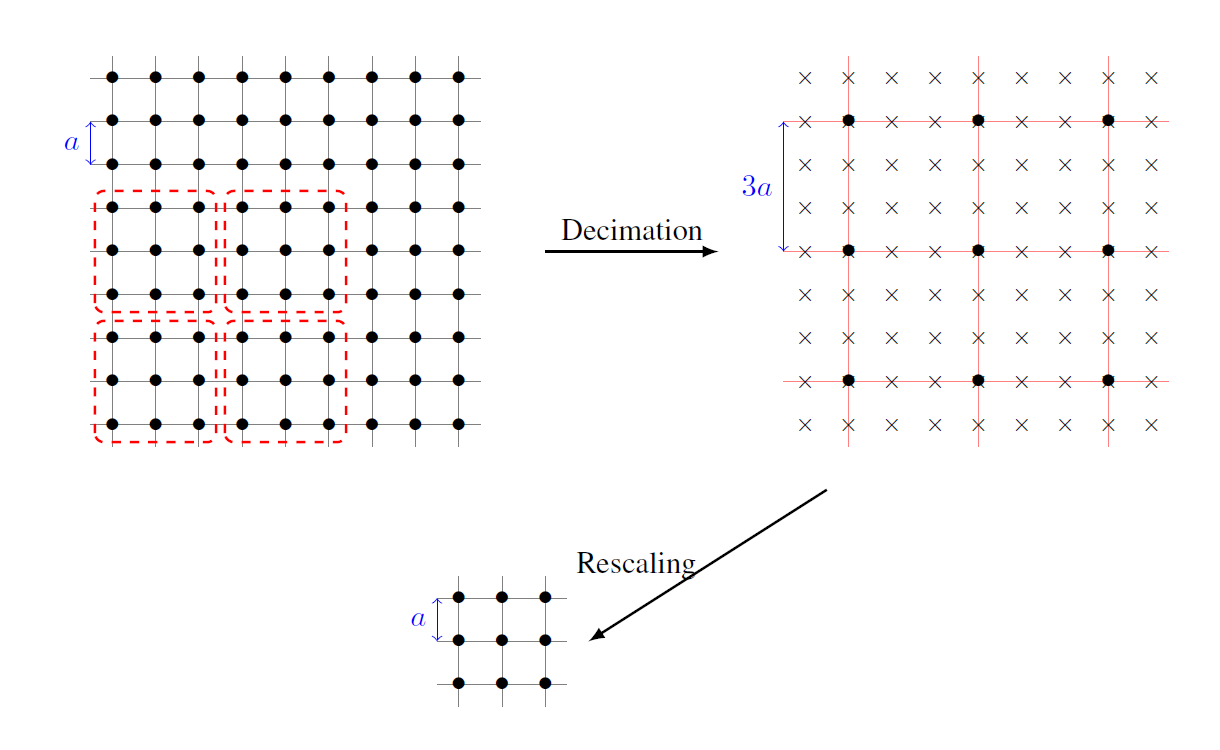
\includegraphics[scale=0.38]{Immagini/kadanoff.png}
\caption{An illustration of the Kadanoff procedure applied on a bidimensional ($D=2$) Ising system with size $a$.
The initial lattice is divided into blocks of size $9$ (so $\alpha = 3$), an effective spin for each block is computated
and an effective spin $S_A$ is obtained. To recover the initial lattice the rescaling $3a\to a$ is performed. \cite{karim}}
\label{fig:ising}
\end{center}
\end{figure}

\subsection{Wilson Momentum shell integration}
The idea of the Kadanoff s block spin can be extended to a system whose degree of freedom are encoded in a field $\phi(x)$,
which we assume to be a continuous function of space and time.

In order to obtain an effective description of the physics of the system in the low momentum (\emph{i.e.}, long distance) regime,
we have to separate the contribution of the modes with momentum higher and lower of a given coarse graining scale $k$:
\begin{equation}
\phi(q) = \phi_< (q) +\phi_> (q)
\end{equation}
The low momentum modes $\phi_<$ and the high momentum ones $\phi_>$ are defined in the following way:
\begin{equation}
 \phi_< (q) = \theta(k-|q|)\phi(q)
\end{equation}
\begin{equation}
\phi_> (q)= \theta(k-|q|)\phi(q)
\end{equation}
In view of that, and recalling the definition of the generating functional in presence of a given ultraviolet cutoff $\Lambda$,
(that is the analogous of the initial lattice space in Kadanoff's model so, in a certain sense, we can say  $\Lambda = a^{-1}$) we have:
\begin{equation}
  Z = \int \prod_{|q| \leq \Lambda}d\phi_q\e^{-S_\Lambda[\phi]} 
\end{equation}
we can write:
\begin{equation}
   Z = \int \prod_{|q| \leq k}\prod_{k\leq |q| \leq \Lambda}d\phi_q\e^{-S_\Lambda[\phi]} = \int \prod_{|q| \leq k }d\phi_q\e^{-S_k[\phi]}=   \int \mathcal{D} \phi_< \e^{-S_k[\phi_<]}
\end{equation}
where the running action (also called the \emph{Wilsonian average action}) is defined in the following way:
\begin{equation}
 \e^{-S_k[\phi_<]} = : \int  \prod_{k\leq |q| \leq \Lambda}d\phi_q\e^{-S_\Lambda[\phi]} =   \int \mathcal{D} \phi_> \e^{-S[\phi]}
\end{equation}
In this way we have arrived to a complicated functional integral equation, describing the dependence of the Wilsonian equation
on the scale parameter $k$. 

When $k=\Lambda$ the running action reduces to the classical bare action, which describes the 
the physics of the system in the ultraviolet limit, conversely when $k \to 0$, all the fluctuations are included in the description
of the model, giving us the complete microscopic quantum field theory.

In the intermediate region we may interpret $S_k$ as an effective action describing under certain approximation the physics at the scale 
$k$. A reason to believe that is the fact that, by definition, only modes with $|q| \approx k$ are active on the scale $\sim k^{-1}$.

When this ideas are implemented, one obtains that the exact evolution equation for $S_k$ depends on a certain cutoff function $K_k(q)$.
The equation describing the evolution of $S_k$ has been derived for the first time in \cite{wilson2} for a smooth cutoff function and
in \cite{cinquantotto} for a sharp cutoff.

The most used version of this evolution equation, with a non specified cutoff function, has been derived by J. Polchinski in  \cite{Polchinski} and reads:
\begin{equation}\label{wilson}
 \partial_kS_k = \frac{1}{2} \int \frac{d^Dq}{(2\pi)^D}\partial_kK_k(q)\left(\frac{\delta^2S_k}{\delta \phi_<(q)\delta \phi_<(-q)}- \frac{\delta S_k}{\delta \phi_<(q)}\frac{\delta S_k}{\delta \phi_<(-q)}\right)
\end{equation}
This equation encodes all the perturbative and nonperturbative effects of the model under consideration, given the bare action $S_\Lambda$.
However some problematic aspects have to be considered in order to use equation \eqref{wilson} for practical purpose. For example, if we want to compute any observable out of the running action $S_k$, we still have to compute the partition function, and that implies a functional integration over the low momenta modes $\phi_<$.

Another problem that arise is the non locality, because in eq.\eqref{wilson} modes of different momenta are coupled together. 


Because of those difficulties related to the Wilson procedure, alternative formulations seem to be desirable.

An alternative approach to functional renormalization that has been developed in recent years 
is due to Wetterich, and  it is focalized on a scale
dependent effective action $\Gamma$, rather than on a scale dependent action.

In this thesis I have used this approach, that will be extensively discussed in the following chapter.



\subsubsection{Fixed Points}
The behavior of an interacting field theory is characterized by a set of scale dependent couplings $g_{i,k}$, that I will define in the following way:
$$ \Gamma_k\left[\phi\right]=\sum_i g_{i,k}\mathcal{O}_{i}\left[\phi\right]$$
Where the $\mathcal{O}_{i,k}$ is an appropriate set of operator that span the space to which the scale dependent effective action belongs to 
and that are compatible with the symmetries of the system. For simplicity I have chosen a basis of operator that does not flows, 
so $\mathcal{O}_i$ is independent of $k$.
Taking the $t$-derivative of the effective action:
$$ \dot{\Gamma}_k\left[\phi\right]=\sum_i \beta_i \mathcal{O}_i\left[\phi\right]$$
we can define the \emph{beta functions}. By definition, the beta function $\beta_i$ associated to the coupling $g_i$ is simply its 
$t$ derivative and it depends on the scale and on the coupling itself.

A fixed point is defined as a point where all the beta functions vanishes:
\begin{equation}
 \beta_i (g_i^*) = 0
\end{equation}
where $g_i^*$ is the $i^{th}$ coupling calculated at the fixed point.

Obviously the fixed points are scale invariant points, 
so if we take it as initial condition of the flow, our theory will remain there at every scale. 
In general a given running theory will have several fixed points or even a continuum of fixed points forming a manifold 
in the coupling space.

Each fixed point has its own \emph{basin of attraction}, which is the set of points in coupling constant space which flow inside  
 it when the effective average action flows, so we can see a fixed point as a point where flow lines start or end.

 The study of the behavior of the flow in the proximity of a given fixed point is usually done defining the \emph{stability matrix} in the following way:
\begin{equation}
\left.\mathcal{M}_{ij} \right|_{g^*}=\frac{\partial {\beta}_i}{\partial {g}_j} 
\end{equation}
This matrix can be diagonalized in order to obtain a set of eigenvalues:
\begin{equation}
 \left.\mathcal{M}_{ij}\right|_{{g}^*}=\text{diag}\left(\omega_1,\omega_2,\dots\right)
\end{equation}
A negative eigenvalue means that the fixed point is attractive in the correspondig direction, the converse is true if the eigenvalue is positive.

\subsubsection{Critical exponents}
If we are following the flow close to the fixed point along the direction $v_i$ (where I have indicated with $v_i$
the eigenvector associated to the $i^{th}$ eigenvalue) the coupling constant can be expressed as the sum of its value
at the fixed point $g_i^*$ plus a small fuctuation around this value:
\begin{equation}
 g_i = g_i^* + \delta g_i
\end{equation}
thus we can linearize the flow equation obtaining:
\begin{equation}\label{expcr}
 \delta \dot{g}_i = \left. \frac{\partial \beta_i}{\partial g_j} \right|_{g^*}\delta g_j = \left.\mathcal{M}_{ij} \right|_{g^*}\delta g_j
\end{equation}
Now we should solve the eigenvalue problem:
\begin{equation}\label{auto}
\left.\mathcal{M}_{ij} \right|_{g^*} v_j^{(a)} = \omega_a v_j^{(a)}
\end{equation}
and expand the coupling constant vector in terms of the basis given by the eigenvector of $\mathcal{M}$:
\begin{equation}\label{c}
 \delta g_i = \sum_a c_a v_i^{(a)}
\end{equation}
where the $c_a$ are some constant to be found.
Now, substituting equation \eqref{c} and \eqref {auto} into the equation \eqref{expcr}, we come to the result:
\begin{equation}
 \dot{c}_a = \lambda_a c_a
\end{equation}
that has the solution:
\begin{equation}
 c_a(t) = c_a(0) \e^{\lambda_a t} = c_a(0)\left(\frac{k}{k_0}\right)^{\lambda_a}
\end{equation}
The \emph{critical exponents}  of the model are defined as:
\begin{equation}
 v_a = -\lambda_a
\end{equation}
and, depending on their sign, the corresponding direction in coupling space is said:
\begin{enumerate}
 \item relevant, if $v_a > 0$;
 \item marginal, if $v_a = 0$;
 \item irrelevan, if $v_a <0$;
\end{enumerate}
In terms of dimensionless quantities (\emph{i.e.} dimensionless couplings) if in the UV a fixed point exist with finite values
of the couplings $g_i^*$ and if there exists a finite number of relevant directions, then the theory is said to be 
renormalizable, even if interacting (this is called \emph{asymptotic safety} \cite{weinberg}).

Yang Mills theories are special cases of asymptotic safety called \emph{asymptotic freedom}, since $g_i^* = 0$ at the fixed point.

 
   %%%%%%%%%%%%%%%%%%%
   %                 %
   %  capitolo2.tex  %
   %                 %
   %%%%%%%%%%%%%%%%%%%

   \chapter{Wetterich's non-perturbative FRG}
\noindent
The \emph{functional renormalization group} (FRG) is an approach to renormalization that combines the functional 
formulation of QFT with Wilson's ideas of renormalization. In the particular approach used in this thesis, introduced 
by \emph{Christof Wetterich}\cite{wetterichprimo}, one uses a scale dependent effective action, called 
\emph{effective average action}, usually indicated with $\Gamma_k$, where $k$ represents a coarse-graining scale, with physical dimension of a momentum.

The effective average action is 
a functional which interpolates between the classical bare action to be quantized, $S$, and the full quantum effective action $\Gamma$.
So, by definition, we have:
\begin{displaymath}
\left\{
\begin{array}{l}
 \Gamma_{k\rightarrow 0} = \Gamma\\
 \Gamma_{k\rightarrow \Lambda} = S
\end{array}
\right.
\end{displaymath}
Where $\Lambda$ is an ultraviolet cutoff, which represent the physical energy scale beyond which  QFT loses its validity.

If $\Lambda$ can be sent to $\infty$, then the quantum field theory is said UV complete.

Physically, $\Gamma_k$ is an effective action for average of fields, the average being taken over a volume $\approx k^{-d}$, 
so the degree of freedom with momenta greater than the coarse-graining scale $k$ are effectively integrated out. 

That renormalization procedure can be formulated directly for a continuum field theory, 
without the needs of a lattice regularization. 

In this chapters I will show how the exact evolution equation for the effective average action can be derived (\emph{i.e.} 
an equation for the derivative of $\Gamma_k$ with respect to $k$), I will discuss its proprieties  and I will mention the two
most common approximation schemes used in the literature that make that equation resolvable. 

\begin{figure}
\begin{center}
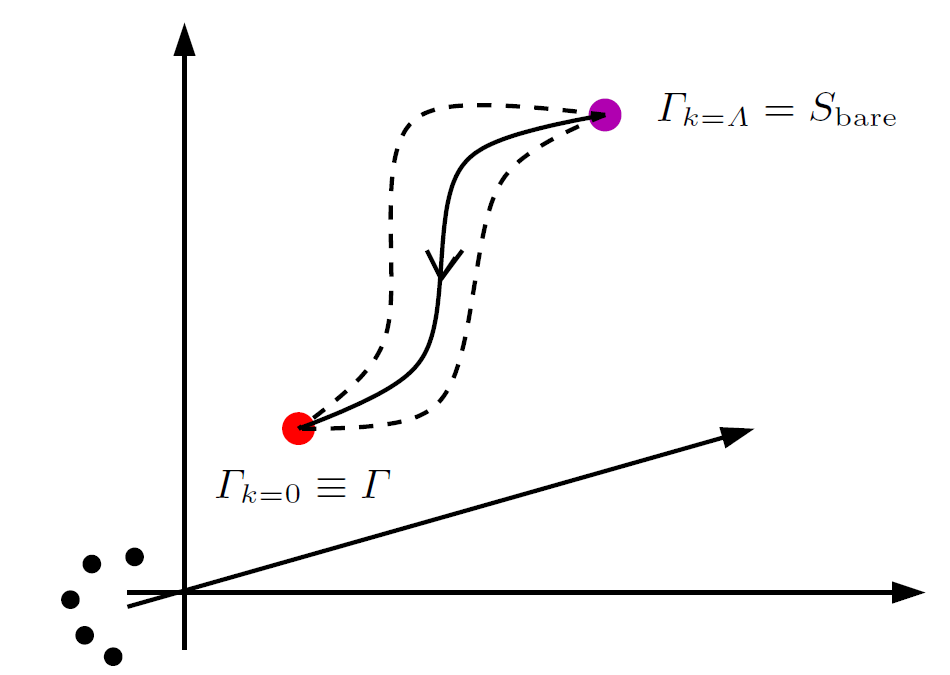
\includegraphics[scale=0.3]{Immagini/azionerunning.png}
\caption{A graphical representation of the renormalization group flow in the space of theories.  Each axis labels a different operator upon which the effective action depends. The functional renormalization group equation determines the evolution of the effective average action $\Gamma_k$, for a given initial condition $\Gamma_\Lambda = S$. A particular trajectory depends on the functional form of the regulator chosen, but all trajectories end at the full quantum action $\Gamma$ when $k\to0$.}
\label{fig:gammaflusso}
\end{center}
\end{figure}


\section{Derivation of the flow equation for $\Gamma_k(\phi_c)$}
The starting point of our treatment is the definition of a non-local regulator term to be added to the classical action:
\begin{equation}
 S_k[\phi] = S[\phi] + \Delta S_k[\phi]
\end{equation}
This term is, by definition,  quadratic in the fields, so it can be written in momentum space as:
\begin{equation}\label{essekappa}
 \Delta S_k[\phi] = \frac{1}{2} \int \frac{d^D q}{(2\pi)^D} \phi(-q)R_k(q)\phi(q)
\end{equation}
Physically, the functional $R_k(q)$ can be interpreted as a momentum-dependent correction to the mass term, and its definition
is the core of all Wetterich's method. According to that definition, we can write the scale dependent generating functional of the Euclidean $n$-point correlation functions $Z_k[J]$:
\begin{equation}\label{wdoppio}
 Z_k[J] \Def \exp \left( -\Delta S_k\left[\frac{\delta}{\delta J}\right] \right) Z_k[J] = \int_{\Lambda} \mathcal{D}\phi \e^{-S[\phi] -\Delta S_k[\phi] + J\cdot\phi}
\end{equation}
where I have defined the dot product between the fields and the classical source in the following way, in coordinate space:
\begin{equation}
 J\cdot\phi = \int d^Dx J_a (x)\phi^a(x)
\end{equation}
or, equivalently:
\begin{equation}
  J\cdot\phi = \int \frac{d^Dq}{(2\pi)^D} J_a (-q)\phi^a(q)
\end{equation}
in momentum space. The scale dependent generating functional of the connected Green function is defined analogously to what 
we've seen in the previous chapter, as the logarithm of $Z_k(\phi)$:
\begin{equation}\label{defW}
 W_k[J] := \ln(Z_k(\phi))
\end{equation}

The primary role of the regulator term is to suppress the contribution of lower modes (the ones inferior to $k$), 
leaving untouched the contribution of the higher ones. The choice of it is almost free. There are just three condition a function must satisfy in order to be coherently
taken as a regulator, conditions that ensure the evolution of $\Gamma_k$ will be well defined in the range $0\leq k\leq\Lambda$. 

As a function of $k$, the regulator function $R_k(q)$ must satisfy the following asymptotic conditions:
\begin{enumerate}
 \item 
 \begin{equation}\label{relazione1}
  \lim_{q^2/k^2 \to 0} R_k(q) > 0
  \end{equation}
       This condition implements the infrared regularization. It ensure that the exact propagator
       $G_k(q^2)$ doesn't diverge when $q^2\to 0$ at vanishing fields. 
       This usually happens because of the contribution of the massless modes, leading to infrared divergences problems. 
       So, that makes $R_k(q)$ an infrared regulator.
\item \begin{equation}\label{relazione2}
       \lim_{k^2/q^2 \to 0} R_k(q) = 0
      \end{equation}
        This condition means that, as it must happens, $Z_{k \to 0}[J] \to Z[J]$ 
       (and, consequently, $\Gamma_{k \to 0}[J] \to \Gamma[J]$), so in this limit the full quantum behavior is recovered.
\item \begin{equation}\label{relazione3}
\lim_{k^2 \to \Lambda^2} R_k(q) \rightarrow \infty
\end{equation}
     When $k$ approaches the ultraviolet cutoff $\Lambda$ the regulator terms causes an exponential suppression of the quantum 
     corrections in the path integral \eqref{wdoppio}, that becomes dominated by the stationary points of the classical action $S$. 
\end{enumerate}
Now we have all we need to derive the \emph{Wetterich equation} or, in other words, the \emph{flow equation for the effective average action}, 
which represent the central tool of the functional renormalization group.

First of all, I will define the \emph{effective average action} in a similar way to what I've done for the effective action in the previous chapter:
\begin{equation}\label{convessa}
 \Gamma_k[\phi_c] = \sup_J \left(\int J\phi_c - W_k[J]\right) - \Delta S_k[\phi]
\end{equation}
where I have also defined the \emph{classical field}:
\begin{equation}\label{otto}
 \phi_c = \langle \phi \rangle = \frac{\delta W_k[J]}{\delta J}
\end{equation}
It's important to note that, because of definition \eqref{otto}, if we define the source as fixed, the field will depend on the scale $k$ and 
\emph{viceversa}. Since later we'll want to study the effective average action as a functional of a fixed classical field, necessarily the classical
source $J$ will be a scale dependent quantity.
Another observation I want to remark is that, because of the terms $\Delta S_k(\phi_c)$, eq.\eqref{convessa} is not mathematically
a Legendre transformation, so $\Gamma_k$ (unlike $\Gamma$) is not necessarily convex. The convexity is obviously recovered in the limit $k\to0$.
\begin{figure}
\begin{center}
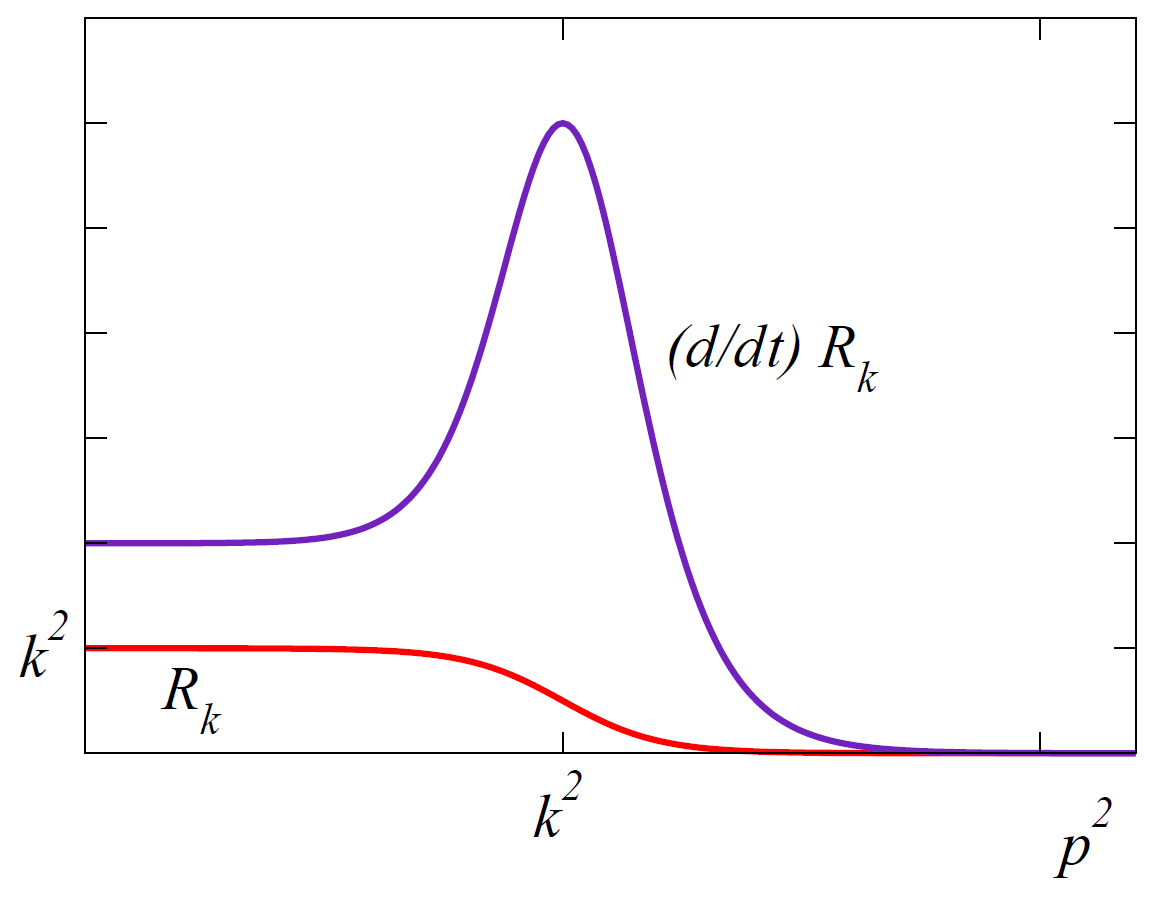
\includegraphics[scale=0.27]{Immagini/redrpunto.png}
\caption{The typical form of a regulator function $R_k$ as a function of $p^2$ (lower curve) and of its derivative $\partial_tR_k$. Due to its finite value for $p^2 \to 0$, the regulator provides for an IR regularization, while its derivative, due to the peaked form we can see plotted in the graph, implements the wilsonian idea of UV regularization by integrating out only fluctuations within a momentum shell near $p^2 \approx k^2$.}
\label{regolatore}
\end{center}
\end{figure}

Differentiating eq.\eqref{convessa} with respect to $k$ we obtain:
\begin{equation*}
 \partial_k \Gamma_k= \int d^D x\partial_kJ(x)\phi_c(x)- \partial_kW_k(J) - \int\frac{\partial W_k[J]}{\partial J(x)}\partial_kJ(x) - \partial_k \Delta S_k[\phi_c]
\end{equation*}
Because of definition \eqref{otto}, the first and the third terms cancel each other and we obtain:
\begin{equation}\label{flussogamma}
 \partial_k \Gamma_k= - \partial_kW_k[J] - \partial_k \Delta S_k[\phi_c]
\end{equation}
Here the derivative of $W[J]$ with respect to $k$ appears. This can be calculated differentiating eq.\eqref{defW} and using eq.\eqref{wdoppio}. The result is:
\begin{equation*}
 \partial_k W_k[J] = -\frac{1}{2}\int d^Dx \int d^Dy\partial_kR_k(x, y)G^{(2)}_k(y,x) - \partial_k\Delta S_k[\phi_c] =
\end{equation*}
\begin{equation}
 = - \frac{1}{2}\Tr(\partial_kR_kG_k^{(2)}) - \partial_k\Delta S_k[\phi_c] 
\end{equation}
where I used the definition of the scale dependent \emph{connected propagator} $G_k(q)$:
\begin{equation}
 G_k = \left( \frac{\delta^2 W_k}{\delta J \delta J}  \right)  =  \langle \phi\phi\rangle -  \langle \phi\rangle \langle\phi\rangle
\end{equation}
If we now substitute this result into eq.\eqref{flussogamma}, we obtain:
\begin{equation}
\partial_k\Gamma_k[\phi_c] = \frac{1}{2}\Tr\big(\partial_kR_kG_k^{(2)}\big)
\end{equation}
What remains to do, now, is to find an expression of the exact propagator in terms of $\Gamma_k$ and of the regulator $R_k$. First of all we notice that, 
because of eq.\eqref{flussogamma}, the quantum equation of motion receives a regulator modification:
\begin{equation}
 J(x) = \frac{\delta\Gamma_k[\phi_c]}{\delta\phi_c(x)} + (R_k\phi)(x)
\end{equation}
From this we have:
\begin{equation}
 \frac{\delta J(x)}{\delta\phi_c(y)} = \frac{\delta^2\Gamma_k[\phi_c]}{\delta\phi_c(x)\delta\phi_c(y)} + R_k(x,y)
\end{equation}
while, from eq.\eqref{otto}, we have:
\begin{equation}
 \frac{\delta\phi_c(y)}{\delta J(x')} = \frac{\delta^2W_k[J]}{\delta J(x')\delta J(y)} = G_k(y-x')
\end{equation}
So we have obtained the following important relation:
\begin{small}
\begin{equation}
 \frac{\delta J(x)}{\delta J(x')} = \delta(x - x') = \int d^D y\frac{\delta J(x)}{\delta \phi_c(y)}\frac{\delta \phi_c}{\delta J(x')} = \int d^D y\left(\frac{\delta^2 \Gamma_k[\phi_c]}{\delta \phi_c(x)\delta \phi_c(y)} + R_k(x,y) \right)G_k(y-x')
\end{equation}
\end{small}
Or, in other words:
\begin{equation}
 G_k(x - y) = \left(\frac{\delta^2 \Gamma_k[\phi_c]}{\delta \phi_c(x)\delta \phi_c(y)} + R_k(x,y)\right)^{-1}
\end{equation}
Collecting everything, we can finally obtain the celebrated \emph{Wetterich's equation}, that describes the flow of the 
effective average action:
\begin{equation}\label{wetterich}
 \dot{\Gamma}_k[\phi_c] \equiv \partial_t\Gamma_k[\phi_c] = \frac{1}{2}\Tr\left\{\partial_tR_k \left(\frac{\delta^2 \Gamma_k[\phi_c]}{\delta \phi_c(x)\delta \phi_c(y)} + R_k(x,y)\right)^{-1}\right\}
\end{equation}
For the sake of convenience, I have defined the adimensional parameter $t$, sometimes called RG time in the literature, in the following way:
\begin{equation}
 t := \ln \left(\frac{k}{\Lambda}\right), \ \ \ \ \ \ \ \ \ \ \ \ \partial_t := k \frac{d}{d k}
\end{equation}

The Wetterich's equation is the starting point of all our future investigations. Here I will spend some words on its proprieties:
\begin{figure}
\begin{center}
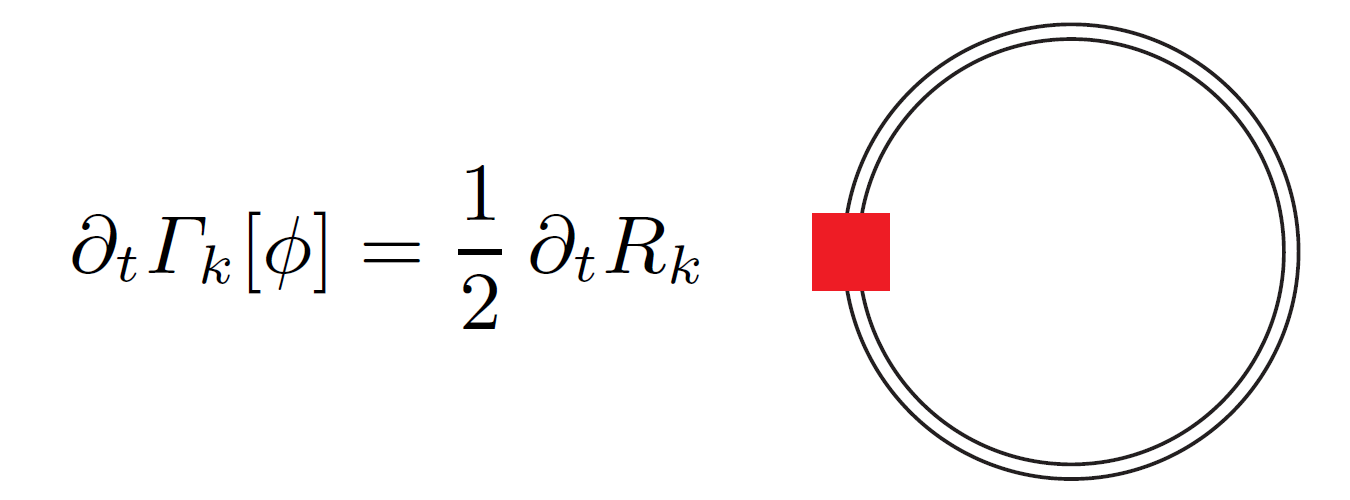
\includegraphics[scale=0.25]{Immagini/flussogamma.png}
\caption{A graphical representation of the Wetterich's equation. The flow of $\Gamma_k$ is given by a one-loop form, which involves the full propagator, represented here by a double line, and the operator $\partial_tR_k$, represented by afilled red box}
\label{fig:gammaflusso}
\end{center}
\end{figure}
\begin{enumerate}
\item This is a functional differential equation, so there are not functional integration to be performed (in contrast with eq.\eqref{wdoppio}).
\item The role of the regulator $R_k$ is twofold: its presence in the denominator of eq.\eqref{wetterich} ensures the infrared regularization, while its derivative $\partial_tR_k$ in the numerator ensures UV regularization, because its support lies on a smeared momentum shell near $p^2 \approx k^2$. This peaked structure of $\partial_tR$ implements nothing but the wilsonian idea of integrating momentum shell by momentum shell and implies that the flow is localized in momentum space. A typical form of a regulator and of its $t$ derivative is depicted in Fig.\ref{regolatore}
\item The Wetterich's equation has a one-loop structure, but it is nevertheless an exact equation, due to the presence of the exact propagator. This structure is the direct consequence of the fact that the regulator term we added to the classical action, $\Delta S_k$, is quadratic in the fields.
\end{enumerate}


\section{Approximations schemes}

The Wetterich's equation, despite its simple form, can't be solved exactly for an arbitrary $\Gamma_k$; that's simply because it
would be technically impossible to find an exact generic solution for a system of infinite coupled integro-differential equations.
So, some approximation on the effective action must be made.

In the following I will discuss the two main approximation method used in the literature: the \emph{vertex expansion} and the \emph{derivative expansion}.
These approximations don't rely on the smallness of a coupling parameter, so the method is, in essence, still  non perturbative. 
The mathematical results of making such approximations is to transform the Wetterich equation into a set of differential equations, 
sometimes much more easy to solve.



\subsection{Vertex expansion}
The vertex expansion approach was introduced and  extensively investigated by Tim R. Morris \cite{verticemorris} and it is widely used in the 
condensed matter physics community and also in low energy QCD studies. It is based upon a truncation of the effective average action in powers of the field:
\begin{equation}
 \Gamma_k[\phi_c] = \sum_{n = 0}^\infty = \frac{1}{n!}\int d^D x_1 \dots d^Dx_n \Gamma_k^{(n)}(x_1, \dots, x_n)\phi_c(x_1)\dots\phi_c(x_n)
\end{equation}
where I have indicated with $\Gamma_k^{(n)}$ the $n^{th}$ order functional derivative of $\Gamma_k$ with respect to the field.
By inserting this into the Wetterich's equation \eqref{wetterich} we obtain the flow equations for the vertex functions $\Gamma_k^{(n)}$, which
can be viewed as a differential FRG form of the Schwinger-Dyson equations.

It has been demonstrated that expanding the effective average action around the field corresponding to  the minimum of $\Gamma_k$ improves 
the convergence proprieties when one is interested in the behavior of the system near phase transitions \cite{verticefasi}.  

\subsection{Derivative Expansion}
In order to obtain approximate solutions of the flow equations, the other main strategy is the derivative expansion of the effective action.
That consists in expanding the effective average action in powers of the gradient of the field. 
This method is often applied to problems where one is interested in low momenta (or, equivalently, long wavelength) behavior,
or when the local structure is known to dominate.

It is the most used approximation technique in the literature and its convergence proprieties has been largely discussed (see, for example, \cite{verticefasi}). 

In this thesis this technique will be applied to the $O(N)$ model, so it will be extensively discussed in the following chapters.
For this reason, I will not spend much words about it now.

\section{Regulator dependence and optimization}
As we have seen, any explicit application of Wetterich's equations requires some approximation and every approximate solutions have a restricted domain of validity.  In addition to that, when approximations are made, the 
independence of physical observables from the choice of the regulator functional is lost. 

If we consider a family of regulators $R_k^{\alpha}(q)$ parametrized by $\alpha$, we are interested in find the particular value of $\alpha$
which minimizes the dependence of the observables of interest from $\alpha$ itself. This translates in the requirement:
\begin{equation}
 \left.\frac{d\mathcal{O}(\alpha)}{d\alpha}\right|_{\alpha = \alpha_{opt}} = 0
\end{equation}
where $\mathcal{O}$ is any physically interesting observable of the model (\emph{e.g.} the effective potential, a critical exponent, etc...).
This idea is called \emph{principle of minimum sensitivity} (PMS) \cite{altrolitim}.

\subsection{Example of regulators}
Various choice of the regulator functional have already been studied in great detail in the literature.
Here I will review the most common ones used and I will discuss the optimal parameter choice in the case of the evolution equation of the effective potential in 
the linear $O(N)$ model in the LPA (local potential approximation) of derivative expansion, which will be studied in depth in the following chapter of this thesis.
In general, because of issues due to numerical calculation, it is preferable to work with the dimensionless rescaled regulator, defined in the following way:
\begin{equation}
 r_k = \frac{R_k(q)}{Z_kq^2}
\end{equation}
where $Z_k$ is the wavefunction renormalization of the model, calculated in the configuration that minimizes the effective potential.
The dimensionless regulator results to be a function only of $q^2/k^2 \Def y$. For the sake of simplicity, I will discuss directly the rescaled regulators in the following.
\begin{enumerate}
 \item Exponential regulator\cite{powerlaw}:
      $$r_{exp}(y) = \frac{a}{\e^{cy^b} - 1}\ \ \ \ \ \  \ \ \ \ \ \ \ \ \ \ b\geq1$$
      In the linear $O(N)$ model treated with the LPA, the optimal parameter choice is $a = 1$, $c = \ln(2)$ and $b = 1.44$.
 \item Power Law regulator\cite{exp}:
      $$r_{pow}(y) = \frac{a}{y^b}$$
      with optimal choice $a = 1$ and $b = 2$.
 \item Litim regulator\cite{litim}:
      $$r_{Lit} (y) = a\left( \frac{1}{y^b} - 1\right)\theta(1-y)$$
      that is a continuous but not differentiable regulator with a compact support. It's one of the most widely used in the literature.
      The optimal choice for the parameters are $a = 1$ and $b = 1$.
 \item CSS regulator\cite{13}:
      $$r_{CSS}(y) = \frac{\exp[{cy_0^b}/({1 - hy_0^b})] - 1}{\exp[{cy^b}/({1 - hy^b})] - 1}\theta(1-hy^b)$$
      It's a very general regulator functional, that recovers all the other ones discussed here as special limits:
      \begin{itemize}
       \item Litim $$\lim_{c\to 0, h\to0} r_{CSS} = \frac{y_0^b}{1 - y_0^b}\left(\frac{1}{y^b} - 1\right) \theta (1 - y)$$
       \item Power Law       $$\lim_{c\to 0, h\to1} r_{CSS} = \frac{y_0^b}{y^b}$$
       \item Exponential $$\lim_{c\to 0, h\to1} r_{CSS} = \frac{\exp[y_0^b] - 1}{\exp[y^b] - 1}$$
      \end{itemize}
\end{enumerate}



\section{Application: the scalar model}
Now I will illustrate the capabilities of the functional renormalization group by a simple but highly 
nontrivial example: the scalar model in $D$ dimensions, described by the following bare action:
\begin{equation}
 S[\phi] = \int d^Dx\left[\frac{Z}{2}\partial^\mu\phi\partial_\mu\phi + V(\phi)\right]
\end{equation}
which now we are going to quantize.
\subsection{The effective potential}
The effective average action is: 
\begin{equation}
 \Gamma_k[\phi] = \int d^D x \left(\frac{Z_k}{2}\partial^\mu \phi \partial_\mu \phi + U_k(\rho) + \mathcal{O}(\partial^2)\right)
\end{equation}
where I have assumed that the effective potential is a function of the field modulus square $\rho = \phi^2/2$. 
Note also that, here and in the following, for the sake of brevity, I will indicate the classical field $\phi_c$ simply with $\phi$. 

I'll use as approximation scheme the derivative expansion in the  LPA' which is, together with LPA, one of the most widely used approximation in the literature.
It consists in keeping only a field independent (but scale dependent) coefficient in the kinetic term, unlike the simpler LPA which consider that term identically equal to one:
\begin{enumerate}
 \item $Z = 1\ \ \ \Longrightarrow$ LPA
 \item $Z = Z_k\ \  \Longrightarrow$ LPA'
\end{enumerate}
The running proper vertices and the Hessian will be calculated for a constant field $\phi_0$, the value which minimizes the effective potential:
\begin{equation}
 \phi(x) \approx \phi_0\ ;\ \ \ \ \ \ U_k\left(\frac{\phi_0^2}{2}\right) = 0
\end{equation}
This is enough if we want to have a first estimate of the functional form of the potential $U_k(\rho)$.

We chose the regulator function to be the \emph{Litim regulator}:
\begin{equation}\label{erre}
 R_k(p^2) = Z_k(k^2 - p^2)\theta(k^2 - p^2)
\end{equation}
\begin{equation}\label{errepunto}
 \dot{R}_k(p^2) = Z_k[(2 - \eta_k)k^2 + \eta_k p^2]\theta(k^2 - p^2)
\end{equation}
Where I have defined the \emph{running anomalous dimension} $\eta = -\dot{Z}_k/Z_k$.
The Hessian of the model, is given by the following expression:
\begin{equation}
 \Gamma_k^{(2)} [\phi, p^2] = Z_k p^2 + U_k^{(2)} (\rho)
\end{equation}

So, substituting it in the Wetterich equation in momentum space we obtain:
\begin{equation*}
 \partial_t U_k(\rho) = \frac{Z_k}{2}\int\frac{d^D p}{(2\pi)^D}\frac{(2 - \eta_k)k^2 + \eta_k p^2}{Z_kk^2 + U_k'(\rho) +  2\rho U_k''(\rho)}\theta(k^2 - p^2) =
\end{equation*}
\begin{equation}
 = Z_k v_D \int_0^{k^2} dp^2\frac{(2-\eta_k)k^2 - \eta_k p^2}{Z_k k^2 + U_k'(\rho) +  2\rho U_k''(\rho)}(p^2)^\frac{D-2}{2}
\end{equation}
where a spherical polar coordinate system was introduced and the spherical symmetry of the integrand used in order to separate the integration in $p$ to the one in the angular coordinates.

I have also defined, for the sake of brevity, the constant $v_D$, in the following way:
\begin{equation*}
 v_D^{-1} = 2^{D+1}\pi^\frac{D}{2}\Gamma\left(\frac{D}{2}\right)
\end{equation*}
The result is easily obtined after some manipulation. It is:
\begin{equation}
 \partial_tU_k(\phi) = \frac{4v_DZ_k(D -\eta_k +2)k^{D + 2}}{Z_k k^2 +  U_k'(\rho) +  2\rho U_k''(\rho)}
\end{equation}
Now it's useful to express the latter equation in terms of dimensionless quantities, so I will define an adimensional potential and an adimensional field 
modulus square, in the following way:
\begin{displaymath}
\left\{
\begin{array}{l}
\widetilde{\rho} = Z_k k^{2-D} \rho \\
u_k({\widetilde{\rho}}) = k^{-D} U_k(\widetilde{\rho})
\end{array}
\right.
\end{displaymath}
So, after some trivial algebraic manipulation, we obtain:
\begin{equation}
\dot{u}(\widetilde{\rho}) = -D  u_k(\widetilde{\rho}) +(D - 2 + \eta)\widetilde{\rho}\frac{\partial u_k(\widetilde{\rho})}{\partial \widetilde{\rho}} + \frac{\pi^{-\frac{D}{2}} (D- \eta_k +2)}{2^{D-1} \Gamma \left(\frac{D}{2}\right)(1 + u_k'(\widetilde{\rho}) + 2 \widetilde{\rho} u_k''(\widetilde{\rho}))}
\end{equation}
Where the following relation has been used:
\begin{equation}
\left.\frac{\partial}{\partial t} U_k(\widetilde{\rho})\right|_{\widetilde{\rho}} = \left.\frac{\partial}{\partial t} [k_Du_k(\widetilde{\rho})]\right|_{\widetilde{\rho}} = k^D\dot{u}(\widetilde{\rho}) + D k^D u_k(\widetilde{\rho})
\end{equation}

\subsection{Anomalous dimension}
To close our set of equation we need also the flow equation for $Z_k$ or, in other words, an explicit expression for the anomalous dimension $\eta_k = -\dot{Z_k}/Z_k$.
This can be easily obtained from the evolution equation of $\Gamma^{(2)}_k(\phi)$ in momentum space. By definition, the expression of $\Gamma_k^{2}(\phi)$ is:
\begin{equation}
{\Gamma}^{(2)}_k(\phi, p^2) = \frac{\delta^2}{\delta \phi(p)\delta\phi^*(p)}{\Gamma}_k(\phi)=Z_kp^2 + U^{(2)}_k(\phi)
\end{equation}
So we have:
\begin{equation}
 Z_k = \frac{1}{V_D}\left.\frac{\partial^2}{\partial p^2}\Gamma_k^{(2)}(\phi, p^2)\right|_{p^2=0}
\end{equation}
and, of course:
\begin{equation}\label{zetaanomala}
 \dot{Z}_k = \frac{1}{V_D}\left.\frac{\partial^2}{\partial p^2}\dot{\Gamma}_k^{(2)}(\phi, p^2)\right|_{p^2=0}
\end{equation}
Where $V_D$ is the $D$- dimensional volume where the system under investigation is confined.
So the starting point of our calculation is the evolution equation for $\Gamma^{(2)}_k$, which can be obtined differentiating
twice the Wetterich's with respect to the fields:
\begin{equation}\label{punto?}
 \dot{\Gamma}_k^{(2)}(\phi) = \frac{1}{2}\Tr\left\{ \dot{R_k}\frac{\delta^2 }{\delta\phi_a\delta\phi_b}\frac{1}{{\Gamma_k}^{(2)} + R_k}\right\} 
\end{equation}
In order to calculate the second functional derivative of the exact propagator:
\begin{equation}
 G_k = \frac{1}{{\Gamma_k}^{(2)} + R_k}
\end{equation}
we use the well known formula for the derivative of a martix knowing its inverse:
\begin{equation}
 \frac{\partial}{\partial x} M^{-1} = - M^{-1}\left(\frac{\partial}{\partial x} M \right) M^{-1}
\end{equation}
And, for the second order derivative:
$$\frac{\partial^2}{\partial x\partial y} M^{-1} = $$
$$M^{-1}\left(\frac{\partial}{\partial x} M \right)M^{-1}\left(\frac{\partial}{\partial y} M \right) M^{-1} + M^{-1}\left(\frac{\partial}{\partial y} M \right)M^{-1}\left(\frac{\partial}{\partial x} M \right) M^{-1} -  M^{-1}\left(\frac{\partial^2}{\partial x\partial y} M \right) M^{-1}$$
So the second functional derivative of the exact propagator is, in coordinate space:
$$ \frac{\delta^2G_k(x_1, x_2)}{\delta \phi(x) \delta \phi(y)} = {G}_k(x_1,  x_3) \left[ 2\frac{\delta {\Gamma^{(2)}}(x_3, x_4)}{\delta \phi(x)}{G_k{(x_4, x_5)}} \frac{\delta {\Gamma_k^{(2)}}(x_5,  x_6)}{\delta \phi(y)} - \frac{\delta^2{\Gamma_k^{(2)}}(x_3, x_6)}{\delta \phi(x) \delta \phi(y)}\right] {G}_k({x_6, x_2})$$
So the trace in \eqref{punto?} becomes:
\begin{equation}
\frac{1}{2}\Tr\left\{ \dot{R_k}\frac{\delta^2 }{\delta\phi_a\delta\phi_b}\frac{1}{{\Gamma_k}^{(2)} + R_k}\right\} = 
\end{equation}
\begin{equation}
 = \left[ {G^{x_1 x_3}}_k \left(\frac{\delta {\Gamma^{(2)x_3 x_4}}_k}{\delta \phi(x)}{G^{x_4x_5}}_k \frac{\delta {\Gamma^{(2)x_5 x_6}}_k}{\delta \phi(y)} - \frac{1}{2}\frac{\delta^2{\Gamma^{(2)x_3x_6}}_k}{\delta \phi(x) \delta \phi(y)}\right) {G^{x_6x_2}}_k \right]{\dot{R_k}^{x_2 x_1}}\equiv A - \frac{1}{2}B
\end{equation}
Where I have used the generalized index notation: the $x_i$ are spacetime coordinate and the integration over repeated index is understood.
I will resolve the two integral separatly. The first one is:
\begin{equation}
\int \prod_{j=1}^6 dx_j G_k(x_3 - x_1) \frac{\delta {\Gamma^{(2)}}_k(x_3, x_4)}{\delta \phi(x)}{G_k(x_5 - x_4)} \frac{\delta {\Gamma^{(2)}(x_5, x_6)}_k}{\delta \phi(y)} G_k(x_2 - x_6)\dot{R_k}(x_1 - x_2) 
\end{equation}
We perform the calculation in momentum space so, we need the momentum-space expression of the quantities in \eqref{p}:
\begin{displaymath}
\left.
\begin{array}{l}
G_k (x_3-x_1) = \int \frac{d^Dq_1}{(2\pi)^D}  \widetilde{G}_k(q_1) e^{i(x_3-x_1)q_1}\\ \\
G_k (x_5-x_4) = \int \frac{d^Dq_2}{(2\pi)^D}  \widetilde{G}_k(q_2) e^{i(x_5-x_4)q_2}\\ \\
G_k (x_2-x_6) = \int \frac{d^Dq_3}{(2\pi)^D}  \widetilde{G}_k(q_3) e^{i(x_2-x_6)q_3}\\ \\
\Gamma^{(3)} (x, x_3, x_4) = \int \frac{d^Dp_1}{(2\pi)^D}\int \frac{d^Dp_2}{(2\pi)^D}\int \frac{d^Dp_3}{(2\pi)^D} \widetilde{\Gamma}^{(3)} \delta (p_1 + p_2 + p_3) e^{ip_1x}e^{ip_2x_3}e^{ip_3x_4}\\ \\	
\Gamma^{(3)} (y, x_5, x_6) = \int \frac{d^Dp'_1}{(2\pi)^D}\int \frac{d^Dp'_2}{(2\pi)^D}\int \frac{d^Dp'_3}{(2\pi)^D} \widetilde{\Gamma}^{(3)} \delta (p'_1 + p'_2 + p'_3) e^{ip'_1y}e^{ip'_2x_5}e^{ip'_3x_6}\\ \\
 \dot{R_k} = [2k^2 Z_k + \dot{Z}_k (k^2 - q^2)]\theta(k^2 - q^2)\\ \\
\end{array}
\right.
\end{displaymath}
Performing the integrations, the following constraints on the momenta are found:
\begin{center}
\begin{tabular}{cc}
$q_1 = q$ & $p_1 = p_1$\\
$q_3 = q$ & $p_1' + p_1 + q$\\
$p_2 = q$ & $p_2 = q$\\
$q_2 = -p_3$ & $p'_2 = -q$\\
$p_1' = q_2$ & $p_3 = -p_1 - q$\\
$p_2' = -q$ & $p_3' = -p_1$
\end{tabular}
\end{center}
After performing a Fourier transform, in order to express the result in momentum space, the following 
expression for the $A$ integral is obtained:
\begin{equation}
 A(p) = V_D\int \frac{d^Dq}{(2\pi)^D}\int\frac{d^Dp}{(2\pi)^D}G_k(q)\Gamma^{(3)}_k(p, q, -p - q)G_k(p+q)\Gamma^{(3)}_k(-p,-q, p+q)G_k(q) \dot{R}_k(q)
\end{equation}
In a similar way the integral $B$ can be evaluated, here I will just state the result:
\begin{equation}
B(p) = V_D \int \frac{d^Dq}{(2\pi)^D} \int\frac{d^Dp}{(2\pi)^D}G_k(q)\Gamma_k^{(4)}(p,-p,q,-q)G_k(q)\dot{R}_k(q)
\end{equation}
These two integrals have an immediate graphical interpretation in terms of two $1$-loop Feynmann diagrams, which I reported in Fig.\ref{fig:grafoA} and in Fig.\ref{fig:grafoB}.
\begin{figure}
\begin{center}
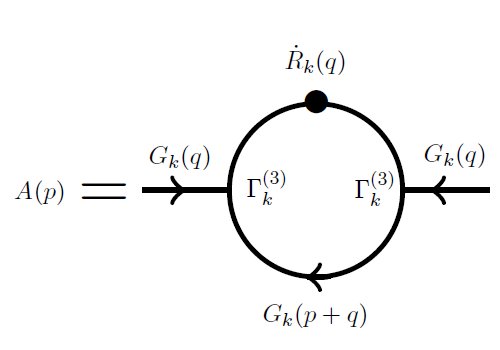
\includegraphics[scale=0.55]{Immagini/grafoA.png}
\caption{Graphical representation of the $A$ integral.}
\label{fig:grafoA}
\end{center}
\end{figure}
Now I will neclet the momentum dependence of the proper vertices, assuming:
$$\Gamma_k^{(3)} \approx 6\sqrt{\rho} U_k''(\rho) + 2\rho^{3/2} U_k'''(\rho)$$
$$\Gamma_k^{(4)} \approx 3\sqrt{\rho} U_k''(\rho) + 12\rho U_k'''(\rho)+ 4\rho^2 U_k''''(\rho)$$

This approximation on the vertices implies the $p$ independence of the $B$ graph, so recalling eq.\eqref{zetaanomala}, 
We come to the conclusion that this one has not influence on the flow equation for $Z_k$. So, putting all the elements
together, we come to the expression:
\begin{equation}\label{241}
 \dot{{Z_k}} =  \left({\Gamma}_k^{(3)}\right)^2 \int \frac{d^Dq}{(2\pi)^D} {G}^2_k(q) \dot{{R}}_k(q)\frac{\partial^2}{\partial p^2}\Big[{G}_k(p + q)\Big]_{p=0}
\end{equation}
In order to simplify the procedure, I will use the identity:
\begin{equation}
 \frac{\partial^2}{\partial p^2}\Big[{G}_k(p + q)\Big]_{p=0} = \frac{\partial^2}{\partial q^2}\Big[{G}_k(q)\Big]
\end{equation}
Now all we have to do is to calculate explicitly the derivative of the exact propagator:
\begin{equation}
\frac{\partial^2}{\partial q^2} \left( Z_k q^2 + U'_k(\rho) + 2\rho U_k''(\rho) + Z_k(k^2 - q^2)\theta(k^2 - q^2)\right)^{-1}
\end{equation}
The Heaviside $\theta$ function allows us to rewrite the preceding expression as a sum of two terms, in the following way:
\begin{equation}
\frac{\partial^2}{\partial q^2} \left(\frac{\theta(k^2 - q^2)}{Z_kk^2 + U'_k(\rho) + 2\rho U_k''(\rho)} +\frac{\theta(q^2 - k^2)}{Z_kq^2 + U'_k(\rho) + 2\rho U_k''(\rho)}\right)
\end{equation}
Performing the first derivative:
\begin{small}
\begin{equation*}
\frac{\partial}{\partial q^\mu}\Big[{G}_k(q)\Big] -\frac{2q_\mu\delta (k^2 - q^2)}{Z_kk^2 + U'_k(\rho) + 2\rho U_k''(\rho)} + \frac{2q_\mu\delta (q^2 - k^2)}{Z_kq^2 + U'_k(\rho) + 2\rho U_k''(\rho)} + \theta(q^2 - k^2) \frac{\partial}{\partial q^\mu}\frac{1}{Z_kq^2 + U'_k(\rho) + 2\rho U_k''(\rho)}
\end{equation*}
\end{small}
The first and the second terms cancel each other, so we have:
\begin{equation}
\frac{\partial}{\partial q^\mu}G_k(q) = - \frac{2q_\mu Z_k\theta(q^2 - k^2)}{\big(Z_k q^2 + U'_k(\rho) + 2\rho U_k''(\rho)\big)^2}
\end{equation}
and, performing the second derivative, we obtain the result:
\begin{equation}
\frac{\partial^2}{\partial q^2}\Big[{G}_k(q)\Big] = 2Z_k\left[ 4\frac{Z_kq^2\theta(q^2 - k^2)}{(Z_kq^2 + U'_k(\rho) + 2\rho U_k''(\rho))^3} - \frac{\theta(q^2 - k^2) + 2q^2 \delta(q^2 - k^2)}{(Z_kq^2 + U'_k(\rho) + 2\rho U_k''(\rho))^2} \right] 
\end{equation}
If we now substitute what we have found in equation \eqref{241} we have, recalling the definition of the Litim optimized regulator \eqref{erre},\eqref{errepunto},
that the terms containing the theta functions don't contribute to the integral, because their support is disjoint from the support of 
the theta function in the definition of $\dot{R}_k(q)$.
\begin{figure}
\begin{center}
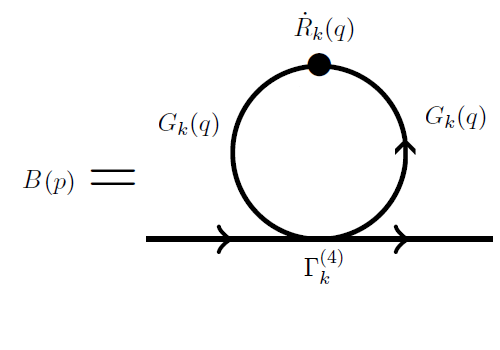
\includegraphics[scale=0.55]{Immagini/grafoB.png}
\caption{Graphical representation of the $B$ integral.}
\label{fig:grafoB}
\end{center}
\end{figure}

So, substituting this result in eq.\eqref{241} and recalling that $\delta(k^2 - q^2)\theta(k^2 - q^2)  = 1/2\delta(k^2 - q^2)$, after some trivial algebrical manipulation, we come to the following expression for the anomalous dimension:
\begin{equation}
  \eta_k = \left.\frac{32 v_D Z_k k^{D + 2}\Big[9\rho\big(U_k''(\rho)\big)^2+ 6 \rho^2 U_k''(\rho)U_k'''(\rho)+ \rho^{3} \big(U_k'''(\rho)\big)^2\Big]}{(Z_kk^2 + U'_k(\rho) + 2\rho U_k''(\rho))^4}\right|_{\rho = \rho_0}
\end{equation}
Where I have named $\rho_0$ the field modulus square at the potential minimun.
Now we should express the latter expression in terms of dimensionless quantities, so I recall the definitions of the adimensional potential and of the adimensional field modulus square:
\begin{displaymath}
\left\{
\begin{array}{l}
\widetilde{\rho} = Z_k k^{2-D} \rho \\
u_k({\widetilde{\rho}}) = k^{-D} U_k(\widetilde{\rho})
\end{array}
\right.
\end{displaymath}
So we obtain:
\begin{equation}
\eta_k = \frac{2^{4-D} \pi ^{-\frac{D}{2}} \left(3 \widetilde{\rho} u_k''(\widetilde{\rho} ) +\rho ^2 u_k'''(\widetilde{\rho} )\right)^2}{\rho  \Gamma \left(\frac{D}{2}\right) (1 + 2 \widetilde{\rho} u_k''(\widetilde{\rho}))^4}
\end{equation}
where all the quantities are calculated at the potential minimum.












     %%%%%%%%%%%%%%%%%%%%
     %                  %
     %  capitolo3.tex   %
     %                  %
     %%%%%%%%%%%%%%%%%%%%
     
\chapter{The $O(N)$ model at $O(\partial^2)$ of the derivative expansion}
\noindent
In this chapter I will apply the concepts illustrated in the previous one to a concrete model, the $O(N)$ model, 
which describes the behavior of an $N$-components real scalar field $\phi^a(x)$ with an $O(N)$ rotational invariance in vector representation. 


Due to its simplicity and to the wide number of physical systems it's able to describe, the $O(N)$ model is one of the most studied in 
modern theoretical physics. 
As an example, I remember here just some of the systems described using that as theoretical framework:
\begin{enumerate}
 \item polymers, for $N = 0$ \cite{polimeri};
 \item the Ising model, for $N = 1$ \cite{ising};
 \item the XY model, for $N = 2$ \cite{xy};
 \item the Heisemberg model, for $N = 3$ \cite{Polyakov};
 \item chiral effective model for QCD, for $N = 4$\cite{hidaka};
 \item theory of high $T_c$ sperconductivity, for $N = 5$\cite{super};
\end{enumerate}
Moreover, also the Higgs field of the Standard Model is based on a linear complex $O(N)$ model.

The approximation scheme I'll use on the \emph{effective average action} in order to solve the Wetterich equation
\eqref{wetterich} is a derivative expansion up to order $O(\partial^2)$ (naturally the derivative expansion is consistent with the $O(N)$ symmetry).
So we have the following expression for $\Gamma_k$:
\begin{equation}\label{azioneefficace}
 \Gamma_k (\phi) = \int d^Dx \left[  U_k(\rho) + \frac{Z_k(\rho)}{2} \partial^\mu \phi_a(x) \partial_\mu \phi^a(x) + \frac{Y_k(\rho)}{4} \partial^\mu \rho(x) \partial_\mu \rho(x) + \mathcal{O}(\partial^4)\right]
\end{equation}
where I have defined $\rho(x) = \frac{1}{2}\phi^a(x)\phi_a(x)$.
The effective potential $U_k(\rho)$ is the observable that permit us to study the ground state of a given theory as well as the basics interactions, while the kinetic term involve two different renormalization functions, $Z_k(\rho)$ and $Y_k(\rho)$.
For $N > 1$ the first one, $Z_k(\rho)$, is related to the renormalization of the Goldstone modes, whereas the renormalization of the radial mode involves both $Z_k(\rho)$ and $Y_k(\rho)$.
To maximally simplify our model we will allow $U_k(\rho)$, $Z_k(\rho)$ and $Y_k(\rho)$ to depends just on $\rho$ and not explicitly on the spacetime position.
In this framework, the evolution equation for $\Gamma_k$ reduces to a system of coupled nonlinear differential equations for the three functions $U_k(\rho)$, $Z_k(\rho)$ and $Y_k(\rho)$.
These evolution equations will be derived in the following, also considering the special case $N\to \infty$,
to eventually study scaling solutions (fixed point configurations of the function space). 


\section{Exact evolution equation for the effective potential}
In order to obtain the FRG flow equation for the effective potential, I will set constant field couplings in the Hessian $\Gamma^{(2)}$.

So, the effective average action is:
\begin{equation}
\Gamma_k(\phi) \approx \int U_k{(\rho)} d^Dx = V_D U_k{(\rho)}
\end{equation}
Where $V_D\equiv\int d^D x$ is the volume in the  $D-$dimensional euclidean space where the physical system under consideration is confined. Now we can trivially obtain the effective potential flow equation:
\begin{equation}\label{esempiosopra}
 \dot{U}_k{(\rho)} = \frac{1}{2V_D} \Tr\left\{ \frac{\dot{R}_k}{{\Gamma_k}^{(2)} + R_k}\right\}
\end{equation}
In momentum space:
\begin{equation}\label{...}
\dot{U}_k(\rho) = \frac{1}{2V_D}\sum_{ab} \int d^Dx \int d^D y \int \frac{d^Dp}{(2\pi)^D} \int \frac{d^Dq}{(2\pi)^D} {G}^{a}_a(p^2)\dot{R}_k(q^2) e ^{i(x-y)(p-q)}
\end{equation}
In order to avoid excessive formalism, I will use the same notation for functions or operators in coordinate space and for their Fourier transform.
So, for example the momentum space expression for the exact propagator and the dotted regulator function appearing in \eqref{esempiosopra} read:
\begin{displaymath}
\left.
\begin{array}{l}
 {G_k}^{ab} (x-y) = \int \frac{d^Dp}{(2\pi)^D} {G}^{ab}(p) e^{i(x-y)p}  \\
  \\
 {\dot{R}_k}^{ba} (y-x) =  \delta^{ba} \int \frac{d^Dq}{(2\pi)^D} \dot{R}_k(q^2) e ^{i(y-x)q}\\

 \end{array} 
\right.
\end{displaymath}
I also remark that, because our model involve real scalar fields in coordinate space, in momentum space we have:
$$\phi_a(q) = \phi^*_a(-q)$$
because of the definition of Fourier transorm: 
$$ \phi_a(q) = \int \phi(x) \e^{iqx}d^Dx$$
In the integral in \eqref{...} I'll introduce the variable $ z = y - x $ and, after performing the $z$ and the $x$ integrals, the result is:
\begin{equation}\label{settte}
\dot{U}_k(\rho) = \sum_{a} \int \frac{d^Dq}{(2\pi)^D} {G}^{a}_{k\ a}(q^2)R_k(q^2)
\end{equation}
To perform the integration in $q$ we will use the polar coordinate system in a $D-$dimensional space:
\begin{equation}
 \int \frac{d^Dq}{(2\pi)^D} = 4v_D \int_0^\infty q^{D-1}dq
\end{equation}
I have already performed the integral over the $D$-dimensional solid angle, because of the angular independence of the integrand \eqref{settte} and
I have also defined, for the sake of brevity, the numerical factor $v_D$:
$$v_D = \frac{1}{2^{D+1}\Gamma(\frac{D}{2})(\pi)^\frac{D}{2}}$$
So the  \eqref{settte} becomes:
\begin{equation}
\dot{U}(\rho) = \sum_{a} 2v_D \int_0^\infty q^{D-1}  {G}^{a}_{k\ a}(q)\dot{R}_k(q^2)dq
\end{equation}
The trace of the exact propagator is:
\begin{equation*}\label{uuu}
 {G}^a_a(q^2) = \Big[\Gamma^{(2)}_k(q^2) + R_k(q^2)\Big]^{-1} = 
\end{equation*}
$$\frac{\delta^a_{a} - \widehat{\phi}^{a}\widehat{\phi}_{a}}{U'_k(\rho) +  Z_k({\rho})q^2 + R_k(q^2) }  + \frac{\widehat{\phi}^{a}\widehat{\phi}_{a}}{ U'(\rho) +  2\bar{\rho}U''_k(\rho)+ [Z_k(\bar{\rho}) + {\rho}Y_k(\bar{\rho})]q^2 + R_k(q^2)} =$$
\begin{equation}\label{vvvvvv}
 \frac{N-1}{U'_k(\rho) +  Z_k({\rho})q^2 + R_k(q^2)}  + \frac{1}{U'(\rho) +  2{\rho}U''_k(\rho)+ [Z_k({\rho}) + {\rho}Y_k({\rho})]q^2 + R_k(q^2)} 
\end{equation}
where I have defined:
\begin{equation}
\widehat{\phi}_{a} = \frac{\bar{\phi}_{a}}{\sqrt{2\bar{\rho}}}
\end{equation}
So $\delta^{ab} - \widehat{\phi}^{a}\widehat{\phi}^{b}$ and $\widehat{\phi}^{a}\widehat{\phi}^{b}$ are the projectors on the longitudinal and on the transverse directions respectively.

We can substitute equation \eqref{vvvvvv} in  \eqref{uuu}, obtaining:
\begin{equation}\label{upunto}
\dot{U}(\rho) =   2v_D  \int_0^\infty q^{D-1}  \dot{R}_k(q^2) \left[  {(N-1)}{G_\perp(q^2)}  + {G_\parallel(q^2)}\right] dq
\end{equation}
Where I have defined, for the sake of simplicity the transverse component of the propagator and the longitudinal one, in the following way:
$$G_\perp (q)= \frac{1}{U'_k(\rho) +  Z_k({\rho})q^2 + R_k(q) } $$
$$G_\parallel (q) = \frac{1}{U'(\rho) + 2\bar{\rho}U''_k(\rho) +  (Z_k({\rho}) + \bar{\rho}Y_k(\bar{\rho}))q^2 + R_k(q)}$$
So the propagator can be written in the following way:
\begin{equation}
 G^{ab}(q) = (\delta^{ab} - \widehat{\phi}^a\widehat{\phi}^b)G_\perp (q) + \widehat{\phi}^a\widehat{\phi}^bG_\parallel (q)
\end{equation}
For $\rho \neq 0$ it's easy to identify the first term as the contribution from the $N-1$ Goldstone bosons and the first one as the contribution from the radial mode.
The exact evolution equation for the effective potential can be interpreted in a graphical way in terms of a $1$-loop Feynman-like diagrams, as shown in Fig.\ref{fig:looppot}.
\begin{figure}
\begin{center}
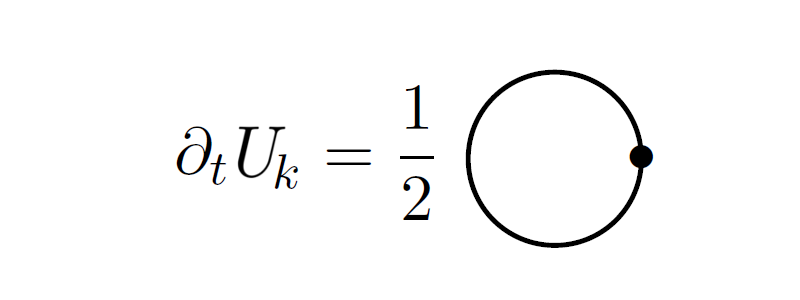
\includegraphics[scale=0.4]{Immagini/potenziale.png}
\caption{A Feynman-like graph representation for the exact evolution equation for the effective potential $U_k(\rho)$.}
\label{fig:looppot}
\end{center}
\end{figure}

In order to study the behavior of the effective potential, an approximation that is widely used in the literature is the LPA (Local Potential Approximation).
The LPA result consists in setting $Z=1$ and $Y=0$.

Although it may seems a crude approximation, the LPA is widely used in many studies, because it qualitatively reproduces most of the properties of the complete functional renormalization group description of the $O(N)$ 
model in the large distance regime, like the stability properties and number of fixed points.


\section{The equations for $\dot{Z}_k(\rho)$ and $\dot{Y}_k(\rho)$}
To go beyond the simple LPA approximation, we need to add the exact evolution equations for the non trivial $Z_k(\rho)$ and $Y_k(\rho)$. 
To derive these equations we need to know the exact evolution equation for the second order functional derivative of the effective average action,
then setting $\rho$ to a constant is sufficient to extract the flow equations.
That is what will be calculated in the following section.

\subsection{Evolution of $\Gamma_k^{(2)}$}
The procedure is very similar to what we've seen for the scalar model in the previous chapter.

The starting point is the \emph{Wetterich equation} \eqref{wetterich}. If we derive it twice with respect to the fields we obtain:
\begin{equation}\label{gamma2dot}
\dot{\Gamma}^{(2)ab}_k(x,y)= \frac{1}{2}\frac{\delta^2 }{\delta\phi_a(x)\delta\phi_b(y)}\Tr\left\{\dot{R_k}G_k\right\} 
\end{equation}
Assuming the field-independence of the functional, our problem is to calculate
the second functional derivative of the exact propagator:
$$G_k = \frac{1}{{\Gamma_k}^{(2)} + R_k}$$
We apply the well-known formula for the derivative of a matrix, knowing the expression of its inverse:
$$\frac{\partial^2}{\partial x\partial y} M^{-1} = $$
$$M^{-1}\left(\frac{\partial}{\partial x} M \right)M^{-1}\left(\frac{\partial}{\partial y} M \right) M^{-1} + M^{-1}\left(\frac{\partial}{\partial y} M \right)M^{-1}\left(\frac{\partial}{\partial x} M \right) M^{-1} -  M^{-1}\left(\frac{\partial^2}{\partial x\partial y} M \right) M^{-1}$$
So the second functional derivative of the exact propagator is:
\begin{equation}\label{trecento11}
 \frac{\delta^2 {G^{x_1 x_2}_{a_1a_2}}_k }{\delta \phi_a(x) \delta \phi_b(y)}= {G^{x_1 x_3}_{a_1a_3}}_k \left[ 2\frac{\delta {\Gamma^{(2)x_3 x_4}_{a_3a_4}}}{\delta \phi_a(x)}{G_{a_4a_5}^{x_4x_5}}_k \frac{\delta {\Gamma_{a_5a_6}^{(2)x_5 x_6}}_k}{\delta \phi_b(y)} - \frac{\delta^2{\Gamma_{a_3a_6}^{(2)x_3x_6}}_k}{\delta \phi_a(x) \delta \phi_b(y)}\right] {G^{x_6x_2}_{a_6a_2}}_k
\end{equation}
So the trace in \eqref{gamma2dot} becomes:
\begin{equation}
\frac{1}{2}\Tr\left\{ \dot{R_k}\frac{\delta^2 }{\delta\phi_a\delta\phi_b}\frac{1}{{\Gamma_k}^{(2)} + R_k}\right\} = 
\end{equation}
\begin{equation}
 = \left[ {G^{x_1 x_3}_{a_1a_3}}_k \left(\frac{\delta {\Gamma^{(2)x_3 x_4}_{a_3a_4}}_k}{\delta \phi_a(x)}{G_{a_4a_5}^{x_4x_5}}_k \frac{\delta {\Gamma_{a_5a_6}^{(2)x_5 x_6}}_k}{\delta \phi_b(y)} - \frac{1}{2}\frac{\delta^2{\Gamma_{a_3a_6}^{(2)x_3x_6}}_k}{\delta \phi_a(x) \delta \phi_b(y)}\right) {G^{x_6x_2}_{a_6a_2}}_k \right]{\dot{R_k}_{a_2a_1}^{x_2 x_1}}\equiv A - \frac{1}{2}B
\end{equation}
Note that the evolution equations for $\Gamma^{(2)}$ involves $\Gamma^{(3)}$ and $\Gamma^{(4)}$. That's a general results, it's possible to demonstrate that the flow equation 
for $\Gamma^{(n)}$ always involves $\Gamma^{(n+1)}$ and $\Gamma^{(n+2)}$.

I'll solve the two integrals $A$ and $B$ separately in the following subsections.

\subsection*{$A$ evaluation}
If we rewrite the generalized sums explicitly in terms of spacetime integrals the expression of $A$  is 
\small{
\begin{equation}\label{quella}
\sum_{a_m}\int \left(\prod_{j=1}^6 dx_j\right) G^{a_1a_3}_k(x_3 - x_1) \frac{\delta {\Gamma^{(2)}_{a_3a_4}}_k(x_3, x_4)}{\delta \phi_a(x)}{G^{a_4a_5}_k(x_5 - x_4)} \frac{\delta {\Gamma^{a_5a_6(2)}(x_5, x_6)}_k}{\delta \phi_b(y)} G^{a_6a_2}_k(x_2 - x_6)\dot{R_k}^{a_2a_1}(x_1 - x_2)
\end{equation}}
First, I'll solve the spacetime integral. It's more convenient to work in momentum space.
The expression for the observable in \eqref{quella}   become:
\begin{displaymath}
\left.
\begin{array}{l}
G_k^{a_1a_3} (x_3-x_1) = \int \frac{d^Dq_1}{(2\pi)^D}  {G}_k^{a_1a_3}(q_1) e^{i(x_3-x_1)q_1}\\ \\
G_k^{a_4a_5} (x_5-x_4) = \int \frac{d^Dq_2}{(2\pi)^D}  {G}_k^{a_4a_5}(q_2) e^{i(x_5-x_4)q_2}\\ \\
G_k^{a_6a_2} (x_2-x_6) = \int \frac{d^Dq_3}{(2\pi)^D}  {G}_k^{a_6a_2}(q_3) e^{i(x_2-x_6)q_3}\\ \\
\Gamma^{(3)aa_3a_4} (x, x_3, x_4) = \int \frac{d^Dp_1}{(2\pi)^D}\int \frac{d^Dp_2}{(2\pi)^D}\int \frac{d^Dp_3}{(2\pi)^D} {\Gamma}^{(3)a_xa_3a_4} \delta (p_1 + p_2 + p_3) e^{ip_1x}e^{ip_2x_3}e^{ip_3x_4}\\ \\	
\Gamma^{(3)ba_5a_6} (y, x_5, x_6) = \int \frac{d^Dp'_1}{(2\pi)^D}\int \frac{d^Dp'_2}{(2\pi)^D}\int \frac{d^Dp'_3}{(2\pi)^D} {\Gamma}^{(3)a_ya_5a_6} \delta (p'_1 + p'_2 + p'_3) e^{ip'_1y}e^{ip'_2x_5}e^{ip'_3x_6}\\ \\
 \dot{R_k}^{a_2a_1} (x_1 - x_2) = \dot{R}_k \delta^{a_1a_2}\\ \\
\end{array}
\right.
\end{displaymath}
Substituting these expressions in \eqref{quella} and performing the spacetime integration we find the
following constraints on the moments:
\begin{center}
\begin{tabular}{cc}
$q_1 = q$ & $p_1 = p_1$\\
$q_3 = q$ & $p_1' + p_1 + q$\\
$p_2 = q$ & $p_2 = q$\\
$q_2 = -p_3$ & $p'_2 = -q$\\
$p_1' = q_2$ & $p_3 = -p_1 - q$\\
$p_2' = -q$ & $p_3' = -p_1$
\end{tabular}
\end{center}
So we can rewrite $A$ in terms of just two momenta, for example $p_1$ and $q$:
\small{
\begin{equation}\label{ja}
 A(x-y) = \sum_{a_m}\int \frac{d^Dq}{(2\pi)^D}\int \frac{d^Dp_1}{(2\pi)^D} {G}_k^{a_1a_3}(q) {\Gamma}^{(3)aa_3a_4}_{(p, q, -p-q)} {G}_k^{a_4a_5}(p_1 + q){\Gamma}^{(3)ba_5a_6}_{(-p,-q,p+q)}{G}_k^{a_6a_2}(q)\dot{R}^{a_2a_1}_k(q) e^{i(x-y)p_1}
\end{equation}}
Now, in order to obtain the momentum-space expresion for $A$ I'll perform a Fourier transform of \eqref{ja}. The result, after performing spacetime integrations in $x$ and $y$, is:
\begin{equation}
 {A}(p)=  \frac{V}{(2\pi)^D}\sum_{a_m} \int \frac{d^Dq}{(2\pi)^D} {G}_k^{a_1a_3}(q) {\Gamma}^{(3)aa_3a_4}_{(p, q, -p-q)} {G}_k^{a_4a_5}(p + q){\Gamma}^{(3)ba_5a_6}_{(-p,-q,p+q)}{G}_k^{a_6a_2}(q)\dot{R}^{a_2a_1}_k(q)
\end{equation}





\subsection*{$B$ evaluation}
The evaluation of $B$ can be performed in the same way.  In coordinate space it is:
\begin{equation}
B(x,y) = \int G^{a_1a_3}_k(x_1,x_3)\frac{\delta^2{\Gamma_{a_3a_6}^{(2)}}_k(x_3,x_6)}{\delta \phi_a(x) \delta \phi_b(y)} G^{a_6a_2}_k(x_6,x_2) \dot{R_k}^{a_2a_1}(x_1,x_2)\prod_{i} d^Dx
\end{equation}
In momentum space it becomes:
\begin{equation*}
{B}(p)= \int\frac{d^Dq}{(2\pi)^D} G^{a_1a_3}_k(q)\frac{\delta^2{\Gamma_{a_3a_6}^{(2)}}(p,-p)}{\delta \phi_a(q) \delta \phi_b(-q)} G^{a_6a_2}_k(q) \dot{R_k}^{a_2a_1}(q)=
\end{equation*}
\begin{equation}
=  \frac{V}{(2\pi)^D} \sum_{a_i}\int \frac{d^Dq}{(2\pi)^D}\ G^{a_1a_3}_k(q)\Gamma_{aba_3a_6}^{(4)}(p,-p,q,-q) G^{a_6a_2}_k(q) \dot{R_k}^{a_2a_1}(q)=
\end{equation}

\ \\


The expression of $\dot{\Gamma}^{(2)}$ in momentum space can trivially obtained by Fourier transform and it reads:
\begin{equation}
\dot{\Gamma}_k^{(2)} (p, p') = \dot{\Gamma}_k^{(2)} (p, p') =\int d^Dxd^Dy\dot{\Gamma}_k^{(2)} (x, y)\e^{ipx}\e^{ip'y} = \frac{V}{(2\pi)^D}\dot{\Gamma}_k^{(2)} (p) \delta(p + p')
\end{equation}
So, putting all together,  we obtain  the expression of $\dot{\Gamma}^{(2)}$:
\begin{equation}
\Gamma^{(2)} = A - \frac{B}{2} = \int \frac{d^Dq}{(2\pi)^D}\Bigg[  -\frac{1}{2} G^{a_1a_3}_k(q)\Gamma_{aba_3a_6}^{(4)}(p,-p,q,-q) G^{a_6a_2}_k(q) \dot{R_k}^{a_2a_1}(q) + 
\end{equation}
\begin{equation}
+ {G}_k^{a_1a_3}(q) {\Gamma}^{(3)aa_3a_4}_{(p, q, -p-q)} {G}_k^{a_4a_5}(p + q){\Gamma}^{(3)ba_5a_6}_{(-p,-q,p+q)}{G}_k^{a_6a_2}(q)\dot{R}^{a_2a_1}_k(q)\Bigg] 
\end{equation}
This equation, expressed as a sum of these two contributions, has an obvious graphical interpretation in terms of the twoFeynman-like graph pictured in Fig.\ref{loops}.

\begin{figure}
\begin{center}
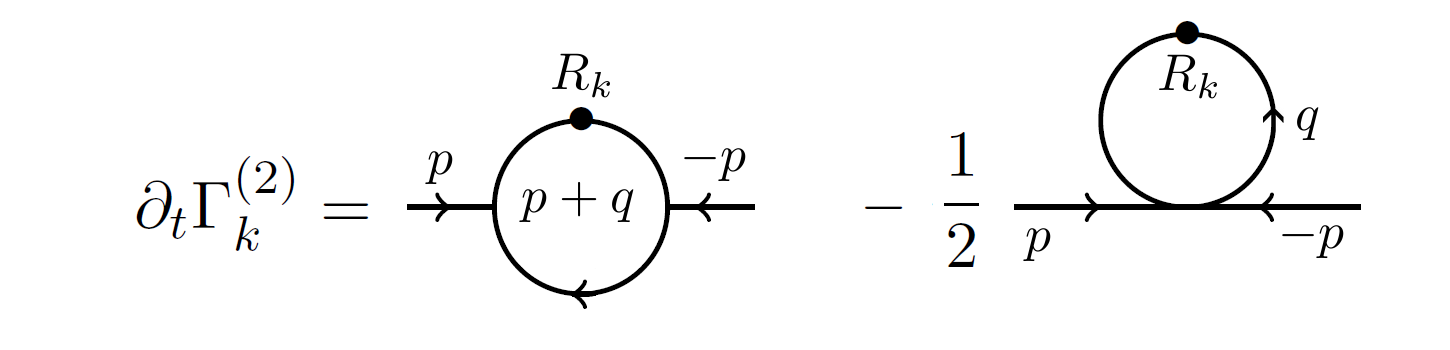
\includegraphics[scale=0.4]{Immagini/grafiloop.png}
\caption{A Feynman-like graph representation for $\Gamma^{(2)} = A - \frac{1}{2} B$}
\label{fig:loops}
\end{center}
\end{figure}

\subsection{Evolution of $Z_k(\rho)$}
Now, in order to perform the calculation of the exact evolution equation of $ Z_k(\rho)$, let's remember the expression of the second functional derivative of the effective average action:
\begin{displaymath}\label{G2}
\left.
\begin{array}{l}
 \frac{\delta^2 \Gamma_{k}}{\delta\phi_a(p)\delta\phi_b(-p)} =  \delta^{ab}U'_k(\rho) + \phi^a\phi^bU''_k(\rho)+ Z_k(\rho) p^2 \delta_{ab} + \rho Y_k(\rho) p^2\widehat{\phi}_a\widehat{\phi}_b  = \\ \\
 = \left[U'_k(\rho) +  Z_k(\rho)p^2\right](\delta_{ab} - \widehat{\phi}_a\widehat{\phi}_b) + \left[U'_k(\rho) + 2\rho U''_k(\rho) + \big(Z_k(\rho) + \rho Y_k(\rho)\big)p^2\right]\widehat{\phi}_a\widehat{\phi}_b\ = \\ \\ 
 \end{array}
\right.
\end{displaymath}
So, if we perform a derivative respect to $p^2$ (the exact meaning of which will be defined in the following) and take the 
longitudinal component of the previous expression, we obtain:
\begin{equation}\label{(42)}
 Z_k(\rho) = \left. \frac{\delta_{ab} - \widehat{\phi}_a\widehat{\phi}_b}{N-1} \frac{\partial}{\partial p^2} \frac{\delta^2 \Gamma_{k}}{\delta\phi_a(p)\delta\phi_b(-p)}\right|_{p = 0} 
\end{equation}
Deriving it with respect to $t = \ln\left(\frac{k}{\Lambda}\right)$ and using equation \eqref{G2} we obtain the following expression for $\dot{Z}_k(\rho)$:
$$\dot{Z}_k(\rho) = \left. \frac{\delta_{ab} - \widehat{\phi}_a\widehat{\phi}_b}{N-1} \frac{\partial}{\partial p^2}     \left(A - \frac{B}{2}\right)        \right|_{p = 0} \Def \dot{Z}^I_k(\rho) + \dot{Z}^{II}_k(\rho)$$
where I have defined $\dot{Z}^I_k(\rho)$ as the first graph contribution to the evolution of $Z_k(\rho)$ and $\dot{Z}^{II}_k(\rho)$ as the contribution due to the second graph. 

I will start from the evaluation of $\dot{Z}^{II}_k(\rho)$:
\begin{equation*}
 \dot{Z}^{II}_k(\rho) = -\frac{\delta_{ab} - \widehat{\phi}_a\widehat{\phi}_b}{2(N-1)} \frac{\partial}{\partial p^2}\left[\int \frac{d^Dq}{(2\pi)^D}G^{a_1a_3}(q)\Gamma^{(4)aba_3a_6}(p, -p, q, -q) G^{a_1a_3}(q)\dot{R}^{a_2a_1}_k(q)\right]_{p=0} = 
\end{equation*}
\begin{equation}\label{zetapunto2}
= -\frac{\delta^{ab} - \widehat{\phi}^a\widehat{\phi}^b}{2(N- 1)}\int \frac{d^Dq}{(2\pi)^D}\dot{R}_k(q)\left[(\delta^{a_3a_6} - \widehat{\phi}^{a_3}\widehat{\phi}^{a_6})G_{\perp}^2 + \widehat{\phi}^{a_3}\widehat{\phi}^{a_6}G_{\parallel}^2 \right]\left(\frac{\partial}{\partial p^2}\Gamma^{(4)}(p,-p,q,-q)\right)
\end{equation}

To go on with the evaluation it is now necessary to calculate the fourth functional derivative respect to the fields of the effective average action
\eqref{azioneefficace}. To simplify as much as possible the problem
we will use what is called the \emph{almost-constant fields approximation}. That consists in considering a large constant background field $\bar{\phi}$ and small 
space-dependent fluctuations around that:
\begin{equation}
 \phi^i(x) = \bar{\phi}^i + \delta \phi^i(x) 
\end{equation}
Concretely, that is equivalent in evaluating the functional derivatives of the effective average action 
(or the \emph{running proper vertices}) putting all the field's spacetime derivatives equal to zero at the end of the calculation.
That is done for every functional derivative of the effective average action up to order four in appendix A. 
It is a very long and tedious calculation, so here I will just state the result for $\Gamma^{(4)}$:
$$\Gamma^{(4)}(p, -p,q, -q) = (\delta^{ab}\delta^{a_3{a_6}} + \delta^{ad}\delta^{bc} + \delta^{ac}\delta^{bd})U_k''(\rho)+(2\rho)^2\widehat{\phi}^a\widehat{\phi}^b\widehat{\phi}^{a_3}\widehat{\phi}^{a_6} +$$
$$+2\rho(\delta^{ab}\widehat{\phi}^{a_3}\widehat{\phi}^{a_6} + \delta^{ad}\widehat{\phi}^b\widehat{\phi}^{a_3} + \delta^{ac}\widehat{\phi}^b\widehat{\phi}^{a_6} + \delta^{bc}\widehat{\phi}^a\widehat{\phi}^{a_6} + \delta^{bd}\widehat{\phi}^a\widehat{\phi}^{a_3} + \delta^{cd}\widehat{\phi}^a\widehat{\phi}^b)U_k'''(\rho) +$$
$$+Z_k'(\rho)\Big[p^2\delta^{ab}\delta^{cd} + 2 p\cdot q(\delta^{ad}\delta^{bc} - \delta^{ac}\delta^{bd}) + q^2\delta^{ab}\delta^{cd}\Big] + $$
$$+2\rho Z_k''(\rho)\Big[p^2\delta^{ab} \widehat{\phi}^{a_3}\widehat{\phi}^{a_6} + p\cdot q(\delta^{ad}\widehat{\phi}^b\widehat{\phi}^{a_3}  - \delta^{ac}\widehat{\phi}^b\widehat{\phi}^{a_6} +\delta^{bc}\widehat{\phi}^a\widehat{\phi}^{a_6} - \delta^{bd}\widehat{\phi}^a\widehat{\phi}^{a_3}) + q^2 \delta^{cd}\widehat{\phi}^a\widehat{\phi}^b \Big] +$$
$$+ \frac{Y_k(\rho)}{2}\Big[p^2(\delta^{ac}\delta^{bd} + \delta^{ac}\delta^{bd}) + q^2(\delta^{bc}\delta^{ad} + \delta^{ac}\delta^{bd}) + 2p\cdot q (\delta^{ac}\delta^{bd} - \delta^{bc}\delta^{ad})\Big] +$$
$$+2\rho^2Y''_k(\rho)(p^2 + q^2)\widehat{\phi}^a\widehat{\phi}^b\widehat{\phi}^{a_3}\widehat{\phi}^{a_6}+\rho Y'_k(\rho)\Big[p^2(\delta^{ac}\widehat{\phi}^b\widehat{\phi}^{a_6} + \delta^{bc}\widehat{\phi}^a\widehat{\phi}^{a_6} + \delta^{ad}\widehat{\phi}^b\widehat{\phi}^{a_3} + \delta^{bd}\widehat{\phi}^a\widehat{\phi}^{a_3} + \delta^{cd}\widehat{\phi}^a\widehat{\phi}^b) + $$
$$p\cdot q(\delta^{ac}\widehat{\phi}^b\widehat{\phi}^{a_6} + \delta^{bd}\widehat{\phi}^a\widehat{\phi}^{a_3} - \delta^{b{a_3}}\widehat{\phi}^a\widehat{\phi}^{a_6} - \delta^{a{a_6}}\widehat{\phi}^b\widehat{\phi}^{a_3}) + $$
$$ + q^2(\delta^{ad}\widehat{\phi}^b\widehat{\phi}^{a_3} +  \delta^{ab}\widehat{\phi}^{a_3}\widehat{\phi}^{a_6} + \delta^{ac}\widehat{\phi}^b\widehat{\phi}^{a_6} + \delta^{bc}\widehat{\phi}^a\widehat{\phi}^{a_6} + \delta^{bd}\widehat{\phi}^a\widehat{\phi}^{a_3})\Big] $$
The $p\cdot q$ terms do not contribute to $\dot{Z}^{II}_k(\rho)$ because of rotational invariance of the space of integration and because the other functions in the integral depends just on $q^2$:
\begin{equation}
 \int\frac{d^Dq}{(2\pi)^D} (p \cdot q)f(q^2) = 0
\end{equation}
Therefore we can ignore the irrelevant $p\cdot q$ terms and perform the $p^2$-derivative of $\Gamma^{(4)}$:
$$\frac{\partial}{\partial p^2}\Gamma^{(4)}(p,-p,q,-q) = Z'_k(\rho)\delta^{ab}\delta^{{a_3}{a_6}} + 2\rho Z''_k(\rho)\delta^{ab}\widehat{\phi}^{a_3}\widehat{\phi}^{a_6} + $$
$$ + \frac{Y_k(\rho)}{2}(\delta^{aa_6}\delta^{ba_3} + \delta^{aa_3}\delta^{ba_6}) + 2\rho^2Y''_k(\rho)\widehat{\phi}^{a}\widehat{\phi}^{b}\widehat{\phi}^{a_3}\widehat{\phi}^{a_6} + $$
\begin{equation}
+\rho Y'_k(\rho)(\delta^{aa_3}\widehat{\phi}^{b}\widehat{\phi}^{a_6} + \delta^{ba_3}\widehat{\phi}^{a}\widehat{\phi}^{a_6} + \delta^{aa_6}\widehat{\phi}^{b}\widehat{\phi}^{a_3} + \delta^{ba_6}\widehat{\phi}^{a}\widehat{\phi}^{a_3} + \delta^{a_3a_6}\widehat{\phi}^{a}\widehat{\phi}^{b})
\end{equation}
Substituting this in equation \eqref{zetapunto2} we obtain, after contracting the $O(N)$ indices:
\begin{equation}
 \dot{Z}_k^{II}(\rho) = -\frac{1}{2}\int\frac{d^Dq}{(2\pi)^D}\dot{R}(q)\left[((N-1)Z'_k(\rho) + Y_k(\rho))G^2_\perp(q) + (Z_k'(\rho) + 2\rho Z''_k(\rho))G^2_\parallel(q)\right]
\end{equation}
The evaluation of the other graph is quite similar. For the sake of brevity I will not rewrite the entire calculation,
but I will only give a sketch of the procedure. The starting point is obviously the expression of $\dot{Z}^{I}_k(\rho)$:
\begin{equation}
\dot{Z}^{I}_k(\rho) = \frac{\delta_{ab} - \widehat{\phi}_a\widehat{\phi}_b}{N-1} \frac{\partial}{\partial p^2}\left[\int \frac{d^Dq}{(2\pi)^D} {G}_k^{a_1a_3}(q) {\Gamma}^{(3)aa_3a_4}_{(p, q, -p-q)} {G}_k^{a_4a_5}(p + q){\Gamma}^{(3)ba_5a_6}_{(-p,-q,p+q)}{G}_k^{a_6a_2}(q)\dot{R}^{a_2a_1}_k(q)\right]_{p=0} =
\end{equation}
Making explicit all the terms in the integrand (the explicit expression of $\Gamma^{(3)}$ in the constant fields approximation and in momentum space can be found in the
Appendix A) and performing the $p^2$ derivative the final result can be derived after a long but not difficult calculation.
In performing the derivative respect to $p^2$ the following identities have been used:
\begin{enumerate}
\item $$ \int\frac{d^Dq}{(2\pi)^D} (p \cdot q)f(q^2) = 0$$
\item $$\int\frac{d^Dq}{(2\pi)^D} (p \cdot q)^2 f(q^2) = \frac{1}{D} \int\frac{d^Dq}{(2\pi)^D} p^2  q^2 f(q^2)$$
\end{enumerate}
and the following series expansion of the propagator:
$$G^{ij}([p+q]^2) = G^{ij}(p^2+2p\cdot q+q^2) = G^{ij}(q^2) + (p^2 + 2p\cdot q)G'^{ij}(q^2))+ 2(p\cdot q)^2G''^{ij}(q^2) + O(p^3)$$
Here $G^{ij}$ is considered as a function of $q^2$ and the primes denote derivatives with respect $q^2$. 
The finale result for $\dot{Z}^{II}_k(\rho)$ is:
\begin{equation}
\dot{Z}^{II}_k(\rho) = \frac{\rho}{D}\int \frac{d^Dq}{(2\pi)^D}\dot{R}_k(q)\Big\{2G^2_\perp(q)G_\parallel(q)(D+2)q^2Y^2_k(\rho)-8Z_k'(\rho)Y_k(\rho)G^2_\perp(q) G_\parallel(q) q^2+
\end{equation}
$$+ 4q^2(Z_k(\rho))^2G^2_\perp(q) G_\parallel(q) + 4DY_k(\rho)U''_k(\rho)G^2_\perp(q) G_\parallel(q) + Y_k^2(\rho)G^2_\perp(q) G'_\parallel(q) (D+8) q^4 - 8Y_k(\rho)Z_k'(\rho)G^2_\perp(q) G'_\parallel(q) q^4+$$
$$+2U''_k(\rho)Y_k(\rho)G^2_\perp(q) G'_\parallel(q) (D+8)q^2 - 16U''_k(\rho)G^2_\perp(q) G'_\parallel(q) Z'_k(\rho)q^2 + 2q^6Y^2_k(\rho)G^2_\perp(q) G_\parallel(q) + $$
$$+ 2Dq^2G^2_\perp(q) G'_\parallel(q) Y_k(\rho)U''_k(\rho) + 4q^4G^2_\perp(q) G''_\parallel(q) U''_k(\rho)Y_k(\rho) +4DG^2_\perp(q) G'_\parallel(q) (U''_k(\rho))^2 + $$
$$+4DG'_\perp(q) G^2_\parallel(q) (U''_k\rho))^2 + 8q^2G''_\perp(q) G^2_\parallel(q) (U''_k(\rho)^2) + 4q^2G_\perp(q) G^2_\parallel(q)(Z'_k(\rho)^2 + 8G^2_\parallel(q) Z'_k(\rho)(DG_\perp(q) +  $$
$$+ Y^2_k(\rho)G^2_\parallel(q)(DG'_\perp(q) + 2q^2G'_\perp(q))U''_k(\rho)) + 8q^2(U''_k(\rho))^2G^2_\perp(q) G''_\parallel(q) +4q^2Y_k(\rho)G^2_\perp(q) G''_\parallel(q) U''_k(\rho)+$$
$$ + 2q^2G''_\perp(q))q^4 + 4G^2_\parallel(q) Y_k(\rho)Z'_k(\rho)(DG_\perp(q) + 2q^2G'_\perp(q)) + 4G^2_\parallel(q) U''_k(\rho)Y_k(\rho)(DG'_\perp(q) + 2q^2G''_\perp(q))q^2$$

\subsection{Evolution of $Y_k(\rho)$}
Instead of deriving the evolution equation of $Y_k(\rho)$ we will calculate the evolution of an equivalent quantity, 
defined in the following way:
\begin{equation}
 \widetilde{Z}_k(\rho) = Z_k(\rho) + \rho Y_k(\rho)
\end{equation}
according to what is usually done in the literature. The evolution equation for $Y_k (\rho)$  can obviously be deduced from the one for $\widetilde{Z}_k(\rho)$ knowing the expression of $Z_k(\rho)$, 
derived in the previous section. From equation \eqref{G2} we obtain:
\begin{equation}\label{(43)}
 \widetilde{Z}_k(\rho) = \left. \widehat{\phi}_a\widehat{\phi}_b \frac{\partial}{\partial p^2} \frac{\delta^2 \Gamma_{k}}{\delta\phi_a(q)\delta\phi_b(-q)}\right|_{p = 0}
\end{equation}
The procedure is exactly the same just seen for $\dot{Z}_k(\rho)$, so I will only state the results:
\begin{equation}
 \dot{\widetilde{Z}}_k(\rho) = \dot{\widetilde{Z}}^{I}_k(\rho) + \dot{\widetilde{Z}}^{II}_k(\rho)
\end{equation}
Where I have separated the two graph contributions:
\small{
$$\dot{\widetilde{Z}}^{I}_k(\rho) = \frac{1}{D} \int\frac{d^Dq}{(2\pi)^D}\dot{R}_k(q) 2\rho \Big\{(N-1)G_\perp^2(q)\big[G_\perp\big(q^2Z'_k(\rho)(DY_k + Z'_k(\rho)) + DY_k(\rho)U''_k(\rho)\big) + $$ 
$$ + (q^2Z'_k(\rho) + U''_k(\rho))\big(2q^2G''_\perp(q)(q^2Z'_k(\rho)+ U''_k(\rho)) + G'_\perp(q^2)((4+D)q^2Z'_k(\rho) + DU''_k(\rho))\big]+$$
$$+ G_\parallel^2(q)\big[G_\parallel(q)(Y_k(\rho) + \rho Y'_k(\rho) + Z'_k(\rho))\Big(q^2\big(Z'_k(\rho) + (2D + 1)(Y'_k(\rho) + \rho Y'_k(\rho) + 2DZ'_k(\rho))\big) + 2D(3U''_k(\rho) + 2\rho U'''_k(\rho))\Big) + $$
$$ + \Big(q^2(Y_k(\rho) + \rho Y'_k(\rho) + 2Z'_k(\rho) + 3U''_k(\rho) + 2\rho U'''_k(\rho)\Big)\Big[G'_\parallel(q)\Big((D+4)q^2(\rho Y'_k(\rho) + Z'_k(\rho)) +D(3U''_k(\rho) + 2\rho U'''_k(\rho))\Big) + $$
$$ + 2q^2\big( \frac{Y_k(\rho)}{2}((4+D)G'_\parallel(q) + 2q^2G''_\parallel(q)) + G''_\parallel (q^2(\rho Y'_k(\rho) + Z'_k(\rho)) + 3U''_k(\rho) + 2\rho U'''_k(\rho))  \big) \Big]\Big\} $$}
and:
\small{
$$\dot{\widetilde{Z}}^{II}_k(\rho) = - \frac{1}{2} \int\frac{d^Dq}{(2\pi)^D}\dot{R}_k(q)\Big[\big(Z'_k(\rho) + \rho Y'_k(\rho)\big)(N-1)G^2_\perp(q) + \big(Z'_k(\rho) + 2\rho Z''_k(\rho) + Y_k(\rho) + 5\rho Y_k'\rho + 2\rho^2 Y''_k(\rho)\big)G^2_\parallel(q) \Big]$$}


\section{Dimensionless quantities}
A fixed point can be defined only in terms of dimensioless quantities, so I have defined the new dimensionless variables, following what is usually done in the literature. All the definitions are summarized in table \ref{tab:DIMENSIONLESS}.


\begin{table}
  \begin{center}
    \begin{small}
      \begin{tabular}{|c|c|c|}

\hline
 \textbf{Symbol}& \textbf{Definition} & \textbf{Description}  \\
\hline
$Z_k$ & $Z_k(\rho_0)$ & wavefunction renormalization at the minimum of the potential\\
\hline
$\rho_0$ & $U'_k(\rho_0) = 0$ & field strength at potential minimum\\
\hline
$\widetilde{\rho}$ & $Z_kk^{2-D}\rho$ & dimensionless field strength \\
\hline
$r(y)$ & $Z^{-1}_k q^{-2}R_k(q)$ & dimensionless regulator\\
\hline
$v_D$ & $[(2^{D + 1}\pi^{D/2}\Gamma(D/2)]^{-1}$ & $v_D$ factor\\
\hline
$y$ & $q^2/k^2$ & dimensionless momentum\\
\hline
$\eta_k$ & $-\dot{Z}_k/Z_k$ & anomalous dimension\\
\hline
$u_k(\widetilde{\rho})$ & $k^{-D}U_k(\widetilde{\rho})$ & renormalized potential\\
\hline
$z_k(\rho)$ & $Z_k(\rho)/Z_k$ & renormalized $Z_k(\rho)$\\
\hline
$\mathcal{Y}_k(\widetilde{\rho})$ & $Z_k^{-2}k^{D-2}Y_k(\rho)$ & renormalized $Y_k(\rho)$\\
\hline
      \end{tabular}
    \end{small}
  \end{center}
\caption{Table of the dimensionless variable used in this thesis, with their definitions and their physical descriptions.}
\label{tab:DIMENSIONLESS}

\end{table}


Now we can rewrite the flow equation in terms of the new variables. 
In the left hand side of all of the flow equations we have a derivative of the observable under examination with respect to $t$, calculated at fixed $\rho$. In order to obtain
an equivalent expression for that flow equation we need to express that in terms of a derivative calculated for a fixed value of $\widetilde{\rho}$.
We have:
\begin{equation*}
 \left. \frac{\partial}{\partial t} \right|_{\widetilde{\rho}} = \left. \frac{\partial}{\partial t} \right|_\rho + \left. \frac{\partial\rho}{\partial t} \right|_{\widetilde{\rho}}\left.\frac{\partial}{\partial\rho}\right|_t =
\end{equation*}
\begin{equation*}
\left.\left. \frac{\partial}{\partial t} \right|_\rho + \left.\left.\frac{\partial\ln{\widetilde{\rho}}}{\partial\ln{\rho}}\right|_t\left.\frac{\partial\ln(\rho)}{\partial t}\right|_{\widetilde{\rho}}\widetilde{\rho}\frac{\partial}{\partial\widetilde{\rho}}\right|_t =  \left. \frac{\partial}{\partial t} \right|_{\rho} + (D- 2 + \eta)\widetilde{\rho}\frac{\partial}{\partial\widetilde{\rho}}\right|_t
\end{equation*}
It will be useful, in the following, also the expression:
\begin{equation}
\frac{\dot{R}_k(q^2)}{Z_k q^2} =  \frac{1}{Z_k}\frac{\partial}{\partial t} \frac{R_k(q^2)}{q^2} = \frac{\partial}{\partial t} r_k(q^2) +\frac{\partial}{\partial t}(\ln Z_k)r(y) =  (\partial_t - \eta) r(y) =  -(2y\partial_y + \eta) r(y)
\end{equation}
The last thing to do is to find a renormalized expression for the two projection of the propagator, $G_\perp(q^2)$ and $G_\parallel(q^2)$.
In order to do this, we will calculated the renormalized expressions for each observable in the definition of those projection.
\begin{enumerate}
 \item $$U_k'(\rho) = \frac{\partial \widetilde{\rho}}{\partial \rho}\partial_{\widetilde{\rho}}[k^Du_k(\widetilde{\rho})] = Z_kk^2u_k'(\widetilde{\rho})$$
 \item $$Z_k(\rho)q^2 = Z_kk^2z_k(\widetilde{\rho})y$$
 \item $$R_k(q^2) = Z_kq^2r_k(q^2) = Z_kk^2r_k(y)y$$
 \item $$2\rho U_k''(\rho) = 2\frac{\widetilde{\rho}}{Z_k k^{2-D}}\left(\frac{\partial\widetilde{\rho}}{\partial{\rho}}\right)^2k^Du''_k(\widetilde{\rho}) = 2Z_kk^2\widetilde{\rho}u''_k(\widetilde{\rho})$$
 \item $$\rho Y_k(\rho)q^2 = \frac{\widetilde{\rho}}{Z_kk^{2-D}}q^2Z_k^2k^{2-D}\mathcal{Y}_k(\widetilde{\rho}) = Z_kk^2\widetilde{\rho}y\mathcal{Y}_k(\widetilde{\rho})$$
\end{enumerate}
So, we have obtained the following expression for the renormalized projections of the exact propagator:
\begin{equation}
 G_\perp(q^2) = \frac{g_\perp(y)}{Z_kk^2}
\end{equation}
\begin{equation}
 G_\parallel(q^2) = \frac{g_\parallel(y)}{Z_kk^2}
\end{equation}
where the dimensionless quantities $g_\perp$ and $g_\parallel$ are defined in the following way:
$$g_\perp(y) = \frac{1}{u_k'(\widetilde{\rho}) + [z_k(\widetilde{\rho}) + r_k(y)]y}$$
$$g_\parallel(y) = \frac{1}{u_k'(\widetilde{\rho}) + 2\widetilde{\rho}u_k''(\widetilde{\rho})+ [z_k(\widetilde{\rho}) + \widetilde{\rho}\mathcal{Y}_k(\widetilde{\rho})+ r_k(y)]y}$$

\subsection{The flow equation for the dimensionless potential}
In order to obtain the flow equation for the dimensionless potential $u_k(\widetilde{\rho})$, first of all we have to rewrite eq.\eqref{upunto} in terms of $\widetilde{\rho}$.
The result is:
\begin{equation}
\left.\frac{\partial}{\partial t} U_k(\widetilde{\rho})\right|_{\widetilde{\rho}} = (D - 2 + \eta)\widetilde{\rho}\frac{\partial U_k(\widetilde{\rho})}{\partial \widetilde{\rho}} + v_dk^{-2} \int_0^\infty (q^2)^{\frac{D}{2}}  \frac{\dot{R}_k(q^2)}{q^2} \left[(N-1)G_\perp(q^2)  + G_\parallel(q^2)\right] d(q^2)
\end{equation}
where I have already changed the integration variable to $q^2$. Now, remembering the definitions of $g_\perp$ and $g_\parallel$, I multiply and divide for $Z_k$ in the integral:
\begin{equation}
\left.\frac{\partial}{\partial t} U_k(\widetilde{\rho})\right|_{\widetilde{\rho}} = (D - 2 + \eta)\widetilde{\rho}\frac{\partial U_k(\widetilde{\rho})}{\partial \widetilde{\rho}} + v_d \int_0^\infty (q^2)^{\frac{D}{2}}  \frac{\dot{R}_k(q^2)}{Z_k (q^2)} \left[ (N-1)g_\perp(q^2)  + g_\parallel(q^2)\right] d(q^2)
\end{equation}
Now we can substitute the dimensionless potential $u_k(\widetilde{\rho}) = k^{-D}U_k(\widetilde{\rho})$. The left hand side becomes:
\begin{equation}
\left.\frac{\partial}{\partial t} U_k(\widetilde{\rho})\right|_{\widetilde{\rho}} = \left.\frac{\partial}{\partial t} [k_Du_k(\widetilde{\rho})]\right|_{\widetilde{\rho}} = k^D\dot{u}(\widetilde{\rho}) + D k^D u_k(\widetilde{\rho})
\end{equation}
So:
\begin{equation}
\dot{u}(\widetilde{\rho}) = -D  u_k(\widetilde{\rho}) +(D - 2 + \eta)\widetilde{\rho}\frac{\partial u_k(\widetilde{\rho})}{\partial \widetilde{\rho}} + v_d \int_0^\infty \frac{(q^2)^{\frac{D}{2}}}{k^D}  \frac{\dot{R}_k(q^2)}{Z_k q^2} \left[  (N-1)g_\perp   + g_\parallel \right] d(q^2) 
\end{equation}
By substituting the definition of $y $ we obtain:
\begin{equation}
\dot{u}(\widetilde{\rho}) = -D  u_k(\widetilde{\rho}) +(D - 2 + \eta)\widetilde{\rho}\frac{\partial u_k(\widetilde{\rho})}{\partial \widetilde{\rho}} + v_d \int_0^\infty y^{\frac{D}{2}}  (\partial_t - \eta) r_k(y) \left[ (N-1){g_\perp}  + g_\parallel \right] dy
\end{equation}
Where I have used the fact that the dimensionless regulator function is function of $y$.

In terms of the threshold function, which I have defined in Appendix C, the flow equation just derived is written in the following way:
\begin{equation}
 \dot{u}(\widetilde{\rho}) = -D  u_k(\widetilde{\rho}) +(D - 2 + \eta)\widetilde{\rho}u'_k(\widetilde{\rho}) + v_d \big((N - 1)L^D_{1,0} + L^D_{0,1} \big)
\end{equation}



\subsection{The flow equation for $z_k(\widetilde{\rho})$}
We can now find the flow equation for the regularized wavefunction renormalization in terms of adimensional quantities.
Obviously, the derivative of $Z_k(\widetilde{\rho})$ becomes:
\begin{equation*}
 \dot{Z}_k(\widetilde{\rho}) = \dot{Z}_k(\rho) + (D-2+\eta)\widetilde{\rho}\frac{\partial}{\partial \widetilde{\rho}}Z_k(\widetilde{\rho})
\end{equation*}
and, substituting the definition of $z_k(\widetilde{\rho})$ and remembering the definitions of the two graphs contributes:
\begin{equation}
\dot{z}_k(\widetilde{\rho}) =  (D-2+\eta)\widetilde{\rho}\frac{\partial}{\partial \widetilde{\rho}} z_k(\widetilde{\rho}) + \eta z_k(\widetilde{\rho}) + \frac{\dot{Z}^I_k(\widetilde{\rho})}{Z_k} + \frac{\dot{Z}^{II}_k(\widetilde{\rho})}{Z_k} 
\end{equation}
Now we have to deduce the renormalized expressions for the two graph. Let's start from $\dot{Z}^{II}_k(\widetilde{\rho})/Z_k$:
\begin{equation*}
 \dot{z}^{II}_k(\widetilde{\rho}) = \frac{\dot{Z}^{II}_k(\widetilde{\rho})}{Z_k} =  -\frac{1}{2Z_k}\int\frac{d^Dq}{(2\pi)^D}\dot{R}(q)\left[((N-1)Z'_k(\rho) + Y_k(\rho))G^2_\perp(q) + (Z_k'(\rho) + 2\rho Z''_k(\rho))G^2_\parallel(q)\right]=
\end{equation*}
\begin{equation*}
=  -v_D\int_0^\infty dx x^{\frac{D}{2}}\frac{\dot{R}(x)}{Z_kx}\left[\left((N-1)\frac{Z_k^2}{k^{D-2}}z'_k(\widetilde{\rho}) + \frac{Z_k^2}{k^{D-2}}\mathcal{Y}_k(\widetilde{\rho})\right)\frac{g^2_\perp(x)}{Z^2_kk^4} + \left(\frac{Z_k^2z'_k(\widetilde{\rho})}{k^{D-2}} + \frac{2\widetilde{\rho} z''_k(\widetilde{\rho})Z_k^2}{k^{D-2}}\right)\frac{g^2_\parallel(x)}{Z^2_kk^4}\right]=
\end{equation*}
\begin{equation}
=  v_D\int_0^\infty dy y^{\frac{D}{2}}  (2y\partial_y + \eta) r_k(y)\left[\left((N-1)z'_k(\widetilde{\rho}) + \mathcal{Y}_k(\widetilde{\rho})\right)g^2_\perp(y) + \left(z'_k(\widetilde{\rho}) + 2\widetilde{\rho} z''_k(\widetilde{\rho})\right)g^2_\parallel(y)\right]
\end{equation}
In a quite similar way, we find the renormalized expression of the other graph:
\begin{equation} 
\dot{z}^{I}_k(\widetilde{\rho}) = \frac{\dot{Z}^{I}_k(\widetilde{\rho})}{Z_k} = 
\end{equation}
$$-\frac{2 \widetilde{\rho}v_D}{D}\int_0^\infty dy(2y\partial_y + \eta_k)r_k(y)\Big\{2g^2_\perp(y)g_\parallel(y)(D+2)y\mathcal{Y}^2_k(\widetilde{\rho})-8z_k'(\widetilde{\rho})\mathcal{Y}_k(\widetilde{\rho})g^2_\perp(y) g_\parallel(y) y+$$
$$+ 4y(z_k(\widetilde{\rho}))^2g^2_\perp(y) g_\parallel(y) + 4D\mathcal{Y}_k(\widetilde{\rho})u''_k(\widetilde{\rho})g^2_\perp(y) g_\parallel(y) + \mathcal{Y}_k^2(\widetilde{\rho})g^2_\perp(y) g'_\parallel(y) (D+8) y^4 - 8\mathcal{Y}_k(\widetilde{\rho})z_k'(\widetilde{\rho})g^2_\perp(y) g'_\parallel(y) y^2+$$
$$+2u''_k(\widetilde{\rho})\mathcal{Y}_k(\widetilde{\rho})g^2_\perp(y) g'_\parallel(y) (D+8)y - 16u''_k(\widetilde{\rho})g^2_\perp(y) g'_\parallel(y) z'_k(\widetilde{\rho})y + 2y^3\mathcal{Y}^2_k(\widetilde{\rho})g^2_\perp(y) g_\parallel(y) + $$
$$+ 2Dyg^2_\perp(y) g'_\parallel(y) \mathcal{Y}_k(\widetilde{\rho})u''_k(\widetilde{\rho}) + 4y^2g^2_\perp(y) g''_\parallel(y) u''_k(\widetilde{\rho})\mathcal{Y}_k(\widetilde{\rho}) +4Dg^2_\perp(y) g'_\parallel(y) (u''_k(\widetilde{\rho}))^2 + $$
$$+4Dg'_\perp(y) g^2_\parallel(y) (u''_k\widetilde{\rho}))^2 + 8yg''_\perp(y) g^2_\parallel(y) (u''_k(\widetilde{\rho})^2) + 4yg_\perp(y) g^2_\parallel(y)(z'_k(\widetilde{\rho})^2 + 8g^2_\parallel(y) z'_k(\widetilde{\rho})(Dg_\perp(y) +  $$
$$+ \mathcal{Y}^2_k(\widetilde{\rho})g^2_\parallel(y)(Dg'_\perp(y) + 2yg'_\perp(y))u''_k(\widetilde{\rho})) + 8y(u''_k(\widetilde{\rho}))^2g^2_\perp(y) g''_\parallel(y) +4y\mathcal{Y}_k(\widetilde{\rho})g^2_\perp(y) g''_\parallel(y) u''_k(\widetilde{\rho})+$$
$$ + 2yg''_\perp(y))y^2 + 4g^2_\parallel(y) \mathcal{Y}_k(\widetilde{\rho})z'_k(\widetilde{\rho})(Dg_\perp(y) + 2yg'_\perp(y)) + 4g^2_\parallel(y) u''_k(\widetilde{\rho})\mathcal{Y}_k(\widetilde{\rho})(Dg'_\perp(y) + 2yg''_\perp(y))y\Big\}$$
In terms of the threshold functions the equation for $\dot{{z}}^{I}_k(\widetilde{\rho})$ and  $\dot{{z}}^{II}_k(\widetilde{\rho})$ are:
$$\dot{z}^{I}_k(\widetilde{\rho}) =  4v_D \widetilde \rho u_k''(\widetilde \rho) Q^{D, 0}_{2, 1} + 4 v_D \mathcal{Y}_k u_k''(\widetilde \rho) Q^{D,1}_{2,1} + v_D \widetilde \rho \mathcal{Y}^2_k (\widetilde \rho)Q^{D,2}_{2,1}- 8 v_D \widetilde \rho z'_k(\widetilde \rho)u_k''(\widetilde \rho)L^D_{1,1}-$$
$$-\frac{4v_D}{D}\big(z_k'(\widetilde \rho)\big)^2\widetilde \rho L^{D+2}_{1,1} - 4v_D \widetilde \rho z_k'(\widetilde \rho) \mathcal{Y}_k(\widetilde \rho)L^{D+2}_{1,1} + \frac{16v_D}{D}\widetilde \rho z_k'(\widetilde \rho) u''_k(\widetilde \rho)N^D_{2,1} + \frac{8v_D}{D} \widetilde \rho z'_k(\widetilde \rho) \mathcal{Y}_k(\widetilde \rho)N^{D+2}_{2,1}$$

$$\dot{z}^{II}_k(\widetilde{\rho}) = - v_D\big[((N-1)z'_k(\widetilde{\rho}) + \mathcal{Y}_k(\widetilde{\rho}\big]L^D_{1,0} - v_D\big[z'_k(\widetilde{\rho}) + 2\widetilde{\rho} z''_k(\widetilde{\rho}\big]L^D_{0,1}$$
\subsection{The flow equation for $\widetilde{z}_k(\widetilde{\rho})$}
The procedure is very similar to what we've just seen for $\dot{z}_k(\widetilde{\rho})$ so here I will omit, for the sake of brevity, 
the details of the calculation, exposing only the final results. For the first graph we have:
$$\dot{\widetilde{z}}_k^{I}(\widetilde{\rho}) \equiv \frac{\dot{\widetilde{Z}}^{I}_k(\rho)}{Z_k} = - \frac{4\widetilde{\rho}v_D}{D} \int_0^\infty y(2y\partial_y + \eta_k)r_k(y) \Big\{(N-1)g_\perp^2(y)\big[g_\perp\big(yz'_k(\widetilde{\rho})(D\mathcal{Y}_k + z'_k(\widetilde{\rho})) + D\mathcal{Y}_k(\widetilde{\rho})u''_k(\widetilde{\rho})\big) + $$ 
$$ + (yz'_k(\widetilde{\rho}) + u''_k(\widetilde{\rho}))\big(2yg''_\perp(y)(yz'_k(\widetilde{\rho})+ u''_k(\widetilde{\rho})) + g'_\perp(y)((4+D)yz'_k(\widetilde{\rho}) + Du''_k(\widetilde{\rho}))\big]+$$
$$+ g_\parallel^2(y)\big[g_\parallel(y)(\mathcal{Y}_k(\widetilde{\rho}) + \widetilde{\rho} \mathcal{Y}'_k(\widetilde{\rho}) + z'_k(\widetilde{\rho}))\Big(y\big(z'_k(\widetilde{\rho}) + (2D + 1)(\mathcal{Y}'_k(\widetilde{\rho}) + \widetilde{\rho} \mathcal{Y}'_k(\widetilde{\rho}) + 2Dz'_k(\widetilde{\rho}))\big) + 2D(3u''_k(\widetilde{\rho}) + 2\widetilde{\rho} u'''_k(\widetilde{\rho}))\Big) + $$
$$ + \Big(y(\mathcal{Y}_k(\widetilde{\rho}) + \widetilde{\rho} \mathcal{Y}'_k(\widetilde{\rho}) + 2z'_k(\widetilde{\rho}) + 3u''_k(\widetilde{\rho}) + 2\widetilde{\rho} u'''_k(\widetilde{\rho})\Big)\Big[g'_\parallel(y)\Big((D+4)y(\widetilde{\rho} \mathcal{Y}'_k(\widetilde{\rho}) + z'_k(\widetilde{\rho})) +D(3u''_k(\widetilde{\rho}) + 2\widetilde{\rho} u'''_k(\widetilde{\rho}))\Big) + $$
$$ + 2y\big( \frac{\mathcal{Y}_k(\widetilde{\rho})}{2}((4+D)g'_\parallel(y) + 2yg''_\parallel(y)) + g''_\parallel (y(\widetilde{\rho} \mathcal{Y}'_k(\widetilde{\rho}) + z'_k(\widetilde{\rho})) + 3u''_k(\widetilde{\rho}) + 2\widetilde{\rho} u'''_k(\widetilde{\rho}))  \big) \Big]\Big\} $$
while, for the other one:
\begin{equation}
 \dot{\widetilde{z}}_k^{II}(\widetilde{\rho}) \equiv \frac{\dot{\widetilde{Z}}^{II}_k(\rho)}{Z_k} =
\end{equation}
$$=  \int_0^\infty dy (2y\partial_y + \eta_k)r_k(y)\Big[\big(z'_k(\widetilde{\rho}) + \widetilde{\rho} \mathcal{Y}'_k(\widetilde{\rho})\big)(N-1)g^2_\perp(y) + \big(z'_k(\widetilde{\rho}) + 2\widetilde{\rho} z''_k(\widetilde{\rho}) + \mathcal{Y}_k(\widetilde{\rho}) + 5\widetilde{\rho} \mathcal{Y}_k' + 2\widetilde{\rho}^2 \mathcal{Y}''_k(\widetilde{\rho})\big)g^2_\parallel(y) \Big]$$
In terms of the threshold functions:
\begin{equation}
\dot{\widetilde{z}}_k^{I}(\widetilde{\rho})= v_D\Big[(N-1)(u_k''(\widetilde \rho))^2\widetilde \rho Q^{D,0}_{3,0} + 4(N-1)\widetilde \rho z'_k(\widetilde \rho)u''_k(\widetilde \rho) Q^{D,1}_{3,0}+
\end{equation}
$$+2(N-1)\widetilde \rho(z'_k(\widetilde \rho))^2 Q^{D,2}_{3,0} + 2\widetilde \rho (3u''_k(\widetilde \rho))+ 2 u_k'''(\widetilde \rho)\widetilde \rho)^2\widetilde Q^{D,0}_{3,0}+$$
$$+4v_D(z'_k(\widetilde \rho) + \mathcal{Y}_k(\widetilde \rho) + \widetilde \rho\mathcal{Y}'_k(\widetilde \rho)) (3u_k''(\widetilde{\rho}) + 2u'''_k(\widetilde{\rho})) \widetilde Q^{D,1}_{3,0}+$$
$$+2v_D(z'_k(\widetilde \rho) + \mathcal{Y}_k(\widetilde \rho) + \widetilde \rho\mathcal{Y}'_k(\widetilde \rho))^2\widetilde Q^{D,2}_{3,0}+\frac{8(N-1)}{D}\widetilde \rho z'_k(\widetilde \rho)u''_k(\widetilde \rho)N^D_{3,0} + $$
$$+\frac{8(N-1)}{D}\widetilde \rho z^2_k(\widetilde \rho)N^{D+2}_{3,0} + \frac{8}{D}(z_k'(\widetilde \rho) + \mathcal{Y}_k(\widetilde \rho) + \widetilde \rho \mathcal{Y}_k(\widetilde \rho))(3 u''_k(\widetilde \rho) + 2 \widetilde \rho u'''_k(\widetilde \rho))\widetilde \rho \widetilde N^D_{3,0} + $$
$$-\frac{8\widetilde \rho}{D}(z'_k(\widetilde \rho) + \mathcal{Y}_k(\widetilde \rho) + \widetilde \rho \mathcal{Y}'_k(\widetilde \rho))^2\widetilde N^{D+2}_{3,0} - 2(N-1) \mathcal{Y}_k(\widetilde \rho) u''_k(\widetilde \rho)  \widetilde \rho L^D_{2,0} -$$
$$-v_D (N-1) \left(z_k'(\widetilde \rho)\mathcal{Y}_k(\widetilde \rho) + \frac{1}{D}\big(z_k'(\widetilde \rho)\big)^2\right)\widetilde \rho L^{D+2}_{2,0}-4\widetilde \rho (z'_k(\widetilde \rho) + \mathcal{Y}_k(\widetilde \rho) + \widetilde \rho \mathcal{Y}'_k(\widetilde \rho))(3 u''_k(\widetilde \rho) + 2 \widetilde \rho u'''_k(\widetilde \rho)) L^D_{0,2} -$$
$$-2v_D\left(2 + \frac{1}{D}\right)\widetilde \rho (z'_k(\widetilde \rho) + \mathcal{Y}_k(\widetilde \rho) + \widetilde \rho \mathcal{Y}'_k(\widetilde \rho))^2L^{D+2}_{0,2} $$
\begin{equation}
 \dot{\widetilde{z}}_k^{II}(\widetilde{\rho}) = v_D\Big[\big(z'_k(\widetilde{\rho}) + \widetilde{\rho} \mathcal{Y}'_k(\widetilde{\rho})\big)(N-1)L^D_{1,0} + \big(z'_k(\widetilde{\rho}) + 2\widetilde{\rho} z''_k(\widetilde{\rho}) + \mathcal{Y}_k(\widetilde{\rho}) + 5\widetilde{\rho} \mathcal{Y}_k' + 2\widetilde{\rho}^2 \mathcal{Y}''_k(\widetilde{\rho})\big)L^D_{0,1} \Big]
\end{equation}




\section{Large N limit}
We are interested now in studying the large N limit, when only transverse (or Goldstone) modes are involved in the dynamic 
of the system. In this limit, as can be easily checked (see, for example, \cite{morristurner}), the flow equation for $Y_k(\rho)$ is decoupled from the other two 
(or, equivalently, $\lim_{N\to \infty} \dot{{\widetilde{Z}}}_k(\rho) = \dot{Z}_k(\rho) $) and the problem simplify considerably.

Now I will derive the large N limits of the two flow equations for the dimensionless effective potential $u_k(\rho)$ and the renormalized wavefunction
renormalization $z_k(\rho)$. Then, these two will be object of a numerical evaluation, which will be started in the following chapter of this thesis.

\subsection{The effective potential evolution in the $N \to\infty$ limit}
In the large $N$ limit, we can keep only the terms of order $N$ in the flow equations. In the case of $\dot{u}_k$ that means:
\begin{equation}
\dot{u}(\widetilde{\rho}) = -D  u_k(\widetilde{\rho}) +(D - 2 + \eta)\widetilde{\rho}\frac{\partial u_k(\widetilde{\rho})}{\partial \widetilde{\rho}} - v_D \int_0^\infty y^{\frac{D}{2}}  (2y\partial_y + \eta_k) r_k(y) (N-1){g_\perp(y)} dy
\end{equation}
In order to perform the limit we need to rescale $u_k(\widetilde\rho)$ and $\rho$:
$$u \to \frac{u}{N} \ \ \ \ \ \ \ \ \ \  \ \ \ \ \ \  \ \ \ \ \ \ \  \ \ \ \ \ \   \widetilde{\rho} \to \frac{\widetilde{\rho}}{N} $$
And so we obtain the following expression:
\begin{equation}\label{upuntolargeN}
\dot{u}_k(\widetilde{\rho}) = -D  u_k(\widetilde{\rho}) +(D - 2 + \eta)\widetilde{\rho}\frac{\partial u_k(\widetilde{\rho})}{\partial \widetilde{\rho}} - v_D \int_0^\infty  \frac{y^{\frac{D}{2}} (2y\partial_y + \eta_k) r_k(y)}{y[z_k(\widetilde{\rho}) + r_k(y)] + u_k'(\widetilde{\rho})} dy 
\end{equation}


\subsection{The flow equation for $w_k(\widetilde{\rho}) \Def u'_k(\widetilde{\rho})$ in the large $N$ limit}
The study of the system in the large $N$ limit can be afford more easily considering, instead of the effective potential $u_k(\widetilde{\rho})$, its derivative $u'_k(\widetilde{\rho})$. Defining $w_k(\widetilde{\rho}) := u'_k(\widetilde{\rho})$ and deriving eq.\eqref{upuntolargeN} with respect to $\widetilde{\rho}$ one obtains:
\begin{equation}\label{wpuntolargeN}
 \dot{w}_k(\widetilde{\rho}) = (\eta_k -2 )w_k(\widetilde{\rho}) + (D-2 +\eta_k)\widetilde{\rho}\frac{\partial w_k(\widetilde{\rho})}{\partial \widetilde{\rho}} + v_D\int_0^\infty dy \frac{y^{\frac{D}{2}}  (2y\partial_y + \eta) r_k(y)(z'_k(\widetilde{\rho})y + w'_k(\widetilde{\rho}))}{\big([z_k(\widetilde{\rho}) + r_k(y)]y + w_k(\widetilde{\rho})\big)^2}
\end{equation}
For the sake of completeness, I will state the latter expression also in terms of the threshold function:
\begin{equation}
 \dot{w}_k(\widetilde{\rho}) = (\eta_k -2 )w_k(\widetilde{\rho}) + (D-2 +\eta_k)\widetilde{\rho}w'_k(\widetilde{\rho}) + v_Dw'_k(\widetilde{\rho})L^D_{1,0} + z'_kL^{D+1}_{1,0}
\end{equation}

\subsection{$z_k(\widetilde{\rho})$ flow equation in the $N \to\infty$ limit}
In the $N \to \infty$ limit, the only non-vanishing term in the exact evolution equation for the renormalized
wavefunction renormalization $z_k(\widetilde{\rho})$ is:
\begin{equation}
\dot{z}_k(\widetilde{\rho}) =\eta z_k(\widetilde{\rho}) + (D-2+\eta)\widetilde{\rho}\frac{\partial}{\partial \widetilde{\rho}} z_k(\widetilde{\rho}) + v_D\int_0^\infty dy y^{\frac{D}{2}}  (2y\partial_y + \eta_k) r_k(x)\left((N-1)z'_k(\widetilde{\rho})\right)g^2_\perp(y) 
\end{equation}
I will go on in analogy to what I've done for the effective potential equation, to perform the $N \to \infty$ limit, I need to rescale $u$ and $\widetilde{\rho}$:
$$u \to \frac{u}{N} \ \ \ \ \ \ \ \ \ \  \ \ \ \ \ \  \ \ \ \ \ \ \  \ \ \ \ \ \   \widetilde{\rho} \to \frac{\widetilde{\rho}}{N} $$
The result is:
\begin{equation}\label{zpuntolargeN}
\dot{z}_k(\widetilde{\rho}) =\eta z_k(\widetilde{\rho}) + (D-2+\eta)\widetilde{\rho}\frac{\partial}{\partial \widetilde{\rho}} z_k(\widetilde{\rho})  + v_D\int_0^\infty dy \frac{y^{\frac{D}{2}}  (2y\partial_y + \eta_k) r_k(y)z'_k(\widetilde{\rho})}{\big([z_k(\widetilde{\rho}) + r_k(y)]y + w_k(\widetilde{\rho})\big)^2}
\end{equation}

  
     %%%%%%%%%%%%%%%%%%%%
     %                  %
     %  capitolo4.tex   %
     %                  %
     %%%%%%%%%%%%%%%%%%%%

\chapter{Some analysis of the fixed point equations}
\noindent
The quest for \emph{fixed points} is essential in any RG-based theory: in quantum field theory, the fixed points structure determine also the nature of the continuum limit and as in statistical physics their nature let control the large distance behavior at criticality.

In the large $N$ limit of the $O(N)$ model, the fixed points are defined as the solutions of the system:
\begin{equation}
\label{sistema}
\left\{
\begin{array}{l}
\dot{w}_k(\widetilde{\rho}) = 0\\
\dot{z}_k(\widetilde{\rho}) = 0\\
\end{array}
\right.
\end{equation}
In this chapter I will start to study the fixed point structure of the $O(N)$ model in the large $N$ limit, in $D=3$ and $D=5$, analyzing the behavior of the derivative of the dimensionless effective potential $w_k(\rho)$ and of the wavefunction renormalization $z_k(\rho)$ in those points, using the
flow equations \eqref{wpuntolargeN} and \eqref{zpuntolargeN} derived in the previous chapter of this thesis. I will distinguish 
between three different situations:

\begin{enumerate}
 \item $\eta_k = 0$ and $z'_k(\widetilde{\rho}) = 0$, already completely studied (see, for example, \cite{vaccascaling}).
 \item $\eta_k \neq 0$ and $z'_k(\widetilde{\rho}) \neq 0$
 \item $\eta_k = 0$ and $z'_k(\widetilde{\rho}) \neq 0$
\end{enumerate}
As I will show, for the first of those cases, analytical exact solutions are available.

In the following I will choose as regulator the \emph{Litim optimized regulator}, discussed in the second chapter of this thesis:
\begin{equation}
R_k(q^2) = Z_k(k^2 - q^2)\theta(k^2 - q^2)
\end{equation}
So, the renormalized one is:
\begin{equation}
{r}_k(y) = \left(\frac{1}{y} - 1\right)\theta(1-y)
\end{equation}
With that choice, the system \eqref{sistema} becomes:
\begin{equation}
\left\{
\begin{array}{l}
(\eta_k -2 )w_k(\widetilde{\rho}) + (D-2 +\eta_k)\widetilde{\rho}\frac{\partial w_k(\widetilde{\rho})}{\partial \widetilde{\rho}} - v_D\int_0^1 dy \frac{y^{\frac{D}{2}-1}    (2-\eta_k + \eta_ky)(z'_k(\widetilde{\rho})y + w'_k(\widetilde{\rho}))}{\big([z_k(\widetilde{\rho}) -1 ]y  +  w_k(\widetilde{\rho})+ 1\big)^2} = 0\\
\eta z_k(\widetilde{\rho}) + (D-2+\eta)\widetilde{\rho}\frac{\partial z_k(\widetilde{\rho})}{\partial \widetilde{\rho}}  -v_D\int_0^1 dy \frac{y^{\frac{D}{2}-1}  (2-\eta_k + \eta_ky) z'_k(\widetilde{\rho})}{\big([z_k(\widetilde{\rho}) -1 ]y  +  w_k(\widetilde{\rho})+ 1\big)^2} = 0
\end{array}
\right.
\end{equation}
For the sake of completeness, I also report the large $N$ limit of the flow equation of the dimensionless effective potential, with our choice of the regulator:
\begin{equation}
 \dot{u}_k(\widetilde{\rho}) = -D  u_k(\widetilde{\rho}) +(D - 2 + \eta)\widetilde{\rho}\frac{\partial u_k(\widetilde{\rho})}{\partial \widetilde{\rho}} - v_D \int_0^\infty  \frac{y^{\frac{D}{2}-1}  (2-\eta_k + \eta_ky) }{y[z_k(\widetilde{\rho}) + r_k(y)] + u_k'(\widetilde{\rho})} dy 
\end{equation}

\section{First case: $\eta_k = 0$ and $z'_k(\rho)= 0$}
If $z_k(\widetilde{\rho})$ is a constant function both of the field strength and of $k$ (the latter is equivalent to the 
requirement of a vanishing anomalous dimension), the flow equation for the renormalized potential \eqref{upuntolargeN} can be solved
in an analytically closed form\cite{1}\cite{12}\cite{13}.

Because of the conditions $\dot{z}_k(\widetilde{\rho}) = 0$ and $z'_k(\widetilde{\rho}) = 0$, we have ${z}_k(\widetilde{\rho}) = 1$, so the system \eqref{sistema} reduces to the single equation:

\begin{equation*}
-2 w_k(\widetilde{\rho}) + (D-2)\widetilde{\rho}\frac{\partial w_k(\widetilde{\rho})}{\partial \widetilde{\rho}} - 2v_D\int_0^1 dy \frac{y^{\frac{D}{2}-1} w'_k(\widetilde{\rho})}{\big([z_k(\widetilde{\rho}) -1 ]y + w_k(\widetilde{\rho})+1\big)^2}  = 
\end{equation*}
\begin{equation}\label{wcase1}
 = -2 w_k(\widetilde{\rho}) + (D-2)\widetilde{\rho}w'_k(\widetilde{\rho}) - \frac{4v_D}{D} \frac{w'_k(\widetilde{\rho})}{\big(w_k(\widetilde{\rho})+1\big)^2}=0
\end{equation}

\subsection{Asymptotic behavior}
In this section I want to study the asymptotic behavior of our system or, in other words, its behavior for $\rho \to \infty$. 

It is easy to see that in this limit the nonlinear differential equation constraints usually the effective potential $u_k(\widetilde{\rho})$ and its derivative $w_k(\widetilde{\rho})$ 
to go to infinity so that the last term in the eq.\eqref{wcase1} is suppressed with respect to the other ones. This happens, for example, 
for the Wilson-Fisher scaling solution for $D= 3$. In general one can write a full asymptotical expansion for the solution.

In order to estract the leading behavior, we can rewrite the large fields limit of eq.\eqref{wcase1} obtaining:
\begin{equation}\label{wasi}
-2 w_k(\widetilde{\rho}) + (D-2)\widetilde{\rho} w'_k(\widetilde{\rho}) = 0
\end{equation}
This equation can be easily integrated giving the following result for the asymptotic behavior of $ w_k(\widetilde{\rho})$:
\begin{equation}\label{wasi}
w_k(\widetilde{\rho}) \approx A \widetilde{\rho}^{\frac{2}{D -2}}
\end{equation}
At last, the asymptotic behavior of the effective potential is recovered integrating this equation with respect to $\widetilde{\rho}$:
\begin{equation}
u_k(\widetilde{\rho}) \approx A' \widetilde{\rho}^{\frac{D}{D -2}}
\end{equation}
One can sistematically compute the subleading term of the asymptotic expansion in powers of $\widetilde{\rho}$.
For example, in $D=3$ the first terms have been calculated and they read:
\begin{equation}
\frac{1}{15 A \rho ^2}-\frac{1}{63 A^2 \rho ^4}+\frac{1}{243 A^3 \rho^6}-\frac{1}{891 A^4 \rho ^8}+\frac{1}{3159 A^5 \rho ^{10}}+\frac{4}{91125 A^5 \rho ^{12}}-\frac{1}{10935 A^6 \rho ^{12}} + \dots 
\end{equation}

\subsection{Fixed points}

A first trivial solution of the fixed point equation \eqref{wcase1} is the so called \emph{Gaussian fixed point}, that is the configuration of a constant potential:
\begin{equation}
 u_k(\widetilde{\rho}) = const\ \ \ \Longrightarrow u'_k(\widetilde{\rho}) = w_k(\widetilde{\rho}) = 0 
\end{equation}

The other, non trivial, solution is found integrating analytically equation \eqref{wcase1} (see, for example, ref. \cite{Marchais}\cite{vaccascaling}).

Here  I will just state the final result.
The solution is expressed in an implicit form, as $ \widetilde{\rho}(w)$ and it reads:
\begin{equation}\label{vacca1}
 \widetilde{\rho}(w) = C' w^{\frac{D}{2} - 1} + \frac{1}{(d + 2)(1 + w)^2} \ _2F_1\left(1, 2, 2 + \frac{D}{2}, \frac{1}{1 + w}\right)
\end{equation}
where $C'$ is an integration constant.
The special function appearing in the fixed point equation \eqref{vacca1} is the \emph{Gauss's Hypergeometric function}, defined by the series expansion \cite{M117}\cite{M118}:
\begin{equation}\label{serieiper}
 \ _2F_1\left(a, b, c, z\right) = \frac{\Gamma(c)}{\Gamma(a)\Gamma(b)}\sum_{n = 0}^{\infty} \frac{\Gamma(a + n)\Gamma(b + n)}{\Gamma(c + n)}\frac{z^n}{n!}
\end{equation}
on the disc $|z| < 1$ and by analytic continuation elsewhere. In addition to that, the serie representation \eqref{serieiper} becomes meaningless  for negative (or zero) 
values of the parameter $c$.
For values of $D$ different from even integers, the fixed points equation \eqref{vacca1} can be written in the most convenient way:
\begin{equation}\label{vacca2}
  \widetilde{\rho}(w) = C w^{\frac{D}{2} - 1} + \frac{1}{(d + 2)} \ _2F_1\left(2, 1 - \frac{D}{2}, 2 - \frac{D}{2}, -w \right)
\end{equation}
where $C' = C - \frac{D\pi}{4 \sin(D\pi/2)}$. The only real solution of equation \eqref{vacca2} that can be extended continuously through $w = 0$
is the one with $C = 0$, which represents what in the literature is called the \emph{Wilson-Fisher fixed point}.
The plots of $w(\widetilde{\rho})$ at the nontrivial fixed point for $D= 3$ and $D=5$ are reported in Fig.\ref{fig:potenziali}.

Note that in $D=5$ the potential is not defined everywhere and there is no physical solution.

%%RICOPIARE ARTICOLO VACCA
\begin{figure}
\begin{center}
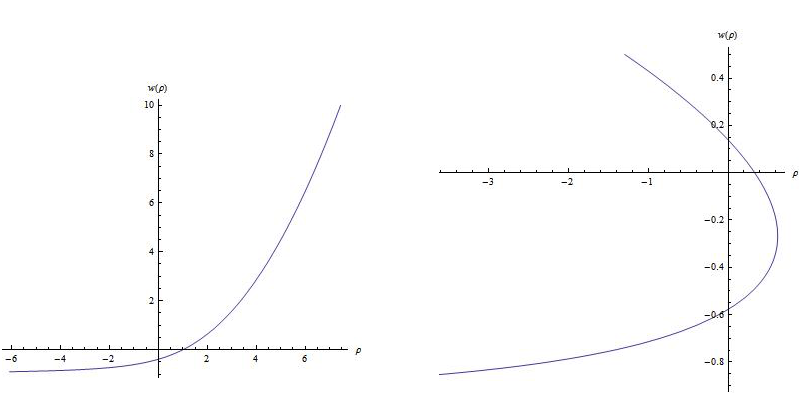
\includegraphics[scale=0.35]{Immagini/potenziali.png}
\caption{A plot of the scaling dimensionless derivative of the potential for $N\to\infty$ in $D=3$ (left) and $D=5$ (right) for $C = 0$ and the optimised Litim regulator.}
\label{fig:potenziali}
\end{center}
\end{figure}
\section{Second case: $\eta_k \neq 0$ and $z'_k(\rho) \neq 0$}
The second case I am going to study is also the most general one, the case of a non constant wavefunction renormalization and of a non vanishing anomalous dimension.
First of all, in order to simplify the notations, I will state some definitions and I will expose the results of some integrals that will be useful in the following.
\subsection{Integrals}
In order to study the flow equations in the most general case, we need to know the explicit expressions of the integrals:
\begin{equation}\label{4ediciotto}
\Int(\alpha) = \int_0^1 dy \frac{y^{\frac{\alpha}{2}}}{\big([z_k(\widetilde{\rho}) -1 ]y  +  w_k(\widetilde{\rho})+ 1\big)^2}
\end{equation}
Because we are interested in the behavior of the model in $D =3$ and in $D=5$, recalling the expressions of the flow equations \eqref{SEDICI},
we need to calculate the following integrals:
\begin{equation}\label{D1}
\Int(1) = - \frac{\tanh ^{-1}\left(\sqrt{\frac{1-z}{w+1}}\right)}{(w+1)^{1/2} (1-z)^{3/2}}+ \frac{1}{(1-z) (w+z)}
\end{equation}
\begin{equation}\label{D3}
\Int(3) = \frac{3 w+2 z+1}{(z-1)^2 (w+z)}-\frac{3 \sqrt{w+1} \tanh ^{-1}\left(\sqrt{\frac{1-z}{w+1}}\right)}{(1-z)^{5/2}}
\end{equation}
\begin{equation}\label{D5}
\Int(5) = \frac{15 w^2+10 w (z+2)-2 (z-7) z+3}{3 (1-z)^3 (w+z)}-\frac{5 (w+1)^{3/2} \tanh ^{-1}\left(\sqrt{\frac{1-z}{w+1}}\right)}{(1-z)^{7/2}}
\end{equation} 
\begin{equation}\label{D7}
\Int(7) = \frac{105 w^3+35 w^2 (2 z+7)-7 w \left(2 z^2-24 z-23\right)+6 z^3-32 z^2+116 z+15}{15 (z-1)^4 (w+z)}-
\end{equation}
\begin{equation*}
 - \frac{7 (w+1)^{5/2} \tanh ^{-1}\left(\sqrt{\frac{1-z}{w+1}}\right)}{(1-z)^{9/2}}
\end{equation*}
Where all the previous solution have validity range $w + z \geq 0$.

Here and in the following, in order to lighten the notations, I have indicated $\widetilde{\rho}$, $w_k(\widetilde{\rho})$, $ z_k(\widetilde{\rho})$ and $\eta_k$  simply with ${\rho}$, $w$, $z$ and $\eta$ respectively.

\subsection{The exact equations}
Now we have all the elements we need in order to write in an useful form the equations:
\begin{equation}\label{SEDICI}
\left\{
\begin{array}{l}
 (\eta -2)w + (D -2 +\eta){\rho} w' - v_D \Big[(2-\eta)w'\Int(D-2) + \big((2-\eta)z' + \eta w'\big)\Int(D) + \eta z'\Int(D + 2)\Big] = 0\\
\eta {z} + (1+\eta)\rho z'  - v_D {z'} \left[(2 - \eta)\Int(D-2) + \eta \Int(D)\right] = 0\\
\end{array}
\right.
\end{equation}
\subsection{Asymptotic behavior}
\subsubsection{Leading order}
In the large field limit, ${\rho} \to \infty$, the second equation of the system \eqref{SEDICI} reduces to:
\begin{equation}
 \eta_k {z({\rho})} + (D-2+\eta){\rho}{z'({\rho})} = 0
\end{equation}
And, by integration, we come to the asymptotic behavior of $z_k$:
\begin{equation}\label{427}
 z({\rho}) \approx B{\rho}^{\frac{-\eta}{D-2+\eta}}
\end{equation}
Where $B$ is an integration constant.
Now, knowing the behavior of $z$ (and, consequently, of $z'$), we can easily see that the integral in the first equation of the system \eqref{SEDICI} becomes 
negligible with respect to the others, so the equation assumes the simplified form:
\begin{equation}
(\eta -2 )w({\rho}) + (D-2 +\eta){\rho} w'({\rho})=0
\end{equation}
at the end we come, after a trivial integration, to the following result:
\begin{equation}\label{429}
w({\rho}) \approx A{\rho}^\frac{2 - \eta}{D - 2 + \eta}
\end{equation}
where $A$ is the integration constant. 
Integrating this with respect to $\rho$, we obtain the asymptotic behavior of the effective potential:
\begin{equation}
u({\rho}) \approx A\frac{D-2+\eta}{D}{\rho}^\frac{D}{D - 2 + \eta}
\end{equation}
In the limit of a vanishing anomalous dimension we note that the results found in the previous section for $u_k$ and $w_k$ are recovered. 
\subsubsection{Next to leading order}
In order to go beyond the leading order (classical) approximations \eqref{427} and \eqref{429}, I had evaluated the first non zero terms in the 
integrals we see in the system \eqref{SEDICI}. 

We know, assuming that $0<\eta<1$, $D>3$ and taking into account the classical solutions just derived in the previous paragraph, that the integrands
of the functions $\Int(\alpha)$ defined in \eqref{4ediciotto} can be approximated, at the leading order, in a neighborhood of the infinity, as:
\begin{equation}
\frac{1}{([z-1]+1+w)^2} \approx \left.\frac{1}{w^2}\right|_{w = A{\rho}^\frac{2 - \eta}{D - 2 + \eta}} + O\big(\rho^{\frac{D-2+\eta}{2(2-\eta)}}\big)
\end{equation}
Now, considering that $z'$ is suppressed with respect to $w'$, the leading corection in the first equation of the system \eqref{SEDICI} is:
\begin{equation}
 v_D\int_0^1 \frac{w'}{w^2} y^{\frac{D}{2}-1} (2-\eta +\eta  y)dy
\end{equation}
so, substituting the leading order expression for $w$ \eqref{429} and its derivative $w'$, we come to the result:
\begin{equation}
 \rho  (D-2 +\eta) w'(\rho )+(\eta -2) w(\rho )=-\frac{v_D \left(4 (\eta -2) (D-\eta +2) \rho ^{-\frac{D}{D+\eta -2}}\right)}{A D (D+2) (D -2 +\eta )}
\end{equation}
and, finally, we come to the next-to-leading order term in $w$:
\begin{equation}
 w(\rho) \approx A \rho ^{\frac{D}{D-2 +\eta}-1}+\frac{ (\eta -2) \rho ^{-\frac{D}{D-2+\eta}}}{A 2^{D+1} \pi ^{\frac{D}{2}}(D-2+\eta) \Gamma \left(\frac{D}{2}+2\right)}
\end{equation}
The first correction to the fixed point equation for $z$ can be derived in a very similar way. We have:
\begin{equation}
 \eta z_k(\widetilde{\rho}) + (D-2+\eta)\widetilde{\rho}z'_k(\widetilde{\rho})  -v_D\int_0^1 \frac{z'}{w^2} y^{\frac{D}{2}-1} (2-\eta +\eta  y)dy = 0
\end{equation}
Substituting the leading order expression of $w$ and $z'$ in the integral and integrating in $y$ we obtain:
\begin{equation}
 \rho  (D -2+\eta) z'(\rho )+\eta  z(\rho )= -\frac{v_D \left(4 B \eta  (D-\eta +2) \rho ^{-\frac{D+2}{D -2+\eta}}\right)}{A^2 D (D+2) (D-2+\eta)}
\end{equation}
this ordinary differential equation can be easily integrated, giving the result:
\begin{equation}
 z(\rho) \approx  B \rho ^{-\frac{\eta }{D+\eta -2}} \left(1+\frac{ \eta  \rho ^{1-\frac{2D}{D+\eta -2}}}{A^22^{D+1} \pi ^{\frac{D}{2}}(D -2+\eta) \Gamma \left(\frac{D}{2}+2\right)}\right)
\end{equation}

\subsection{Equations in $D=3$}
In $D=3$, recalling that $v_3 = (8\pi^2)^{-1}$, the system \eqref{SEDICI} reduces to:
\begin{equation}
\left\{
\begin{array}{l}
 (\eta -2)w + (1 +\eta){\rho} w' - \frac{1}{8\pi^2}\Big[(2-\eta)w'\Int(1) + \big((2-\eta)z' + \eta w'\big)\Int(3) + \eta z'\Int(5)\Big] = 0\\
\eta {z} + (1+\eta)\rho z'  - \frac{z'}{8\pi^2} \left[(2 - \eta)\Int(1) + \eta \Int(3)\right] = 0\\
\end{array}
\right.
\end{equation}
Using equations \eqref{D1}, \eqref{D3} and \eqref{D5} we obtain:
\begin{displaymath}
\left\{
\begin{array}{l}

(\eta -2)w + (1 +\eta){\rho} w' - \frac{1}{8\pi^2}\Bigg[(2-\eta)w'\Big(-\frac{\tanh ^{-1}\left(\sqrt{\frac{1-z}{w+1}}\right)}{(w+1)^{1/2} (1-z)^{3/2}}+\frac{1}{(1-z) (w+z)}\Big) +\\
+\big((2-\eta)z' + \eta w'\big)\Big( \frac{3 w+2 z+1}{(z-1)^2 (w+z)}-\frac{3 \sqrt{w+1} \tanh ^{-1}\left(\sqrt{\frac{1-z}{w+1}}\right)}{(1-z)^{5/2}}\Big) +\\
+ \eta z'\Big(\frac{15 w^2+10 w (z+2)-2 (z-7) z+3}{3 (1-z)^3 (w+z)}-\frac{5 (w+1)^{3/2} \tanh ^{-1}\left(\sqrt{\frac{1-z}{w+1}}\right)}{(1-z)^{7/2}}\Big)\Bigg] = 0\\
\\\eta {z} + (1+\eta)\rho{z'}  - \frac{{z'}}{8\pi^2} \left[(2 - \eta) \left(\frac{\tanh ^{-1}\left(\sqrt{\frac{1-z}{w+1}}\right)}{(w+1)^{1/2} (1-z)^{3/2}}-\frac{1}{(1-z) (w+z)}\right) + \right. \\ 
+\left.  \eta \left(\frac{3 w+2 z+1}{(z-1)^2 (w+z)}-\frac{3 \sqrt{w+1} \tanh ^{-1}\left(\sqrt{\frac{1-z}{w+1}}\right)}{(1-z)^{5/2}}\right)\right] = 0\\
\end{array}
\right.
\end{displaymath}
if $ w + z \geq 0$ and $0<z<1$.

\subsection{Equations in $D=5$}
In $D = 5$, recalling that $v_5 = (48\pi^3)^{-1}$, the system \eqref{SEDICI} becomes:
\begin{equation}
\left\{
\begin{array}{l}
 (\eta -2)w + (1 +\eta){\rho} w' - \frac{1}{48\pi^3}\Big[(2-\eta)w'\Int(3) + \big((2-\eta)z' + \eta w'\big)\Int(5) + \eta z'\Int(7)\Big] = 0\\
\eta {z}+ (3+\eta)\rho{z'}   - \frac{{z'}}{48\pi^3} \left[(2 - \eta)\Int(3) + \eta \Int(5)\right] = 0\\
\end{array}
\right.
\end{equation}
Using equations \eqref{D3}, \eqref{D5} and \eqref{D7} we obtain:
\begin{equation} 
\left\{
\begin{array}{l}
 (\eta -2)w + (1 +\eta){\rho} w' - \frac{1}{48\pi^3}\Big[(2-\eta)w'\left(\frac{3 w+2 z+1}{(z-1)^2 (w+z)}-\frac{3 \sqrt{w+1} \tanh ^{-1}\left(\sqrt{\frac{1-z}{w+1}}\right)}{(1-z)^{5/2}}\right) +\\
 + \big((2-\eta)z' + \eta w'\big)\left(\frac{15 w^2+10 w (z+2)-2 (z-7) z+3}{3 (1-z)^3 (w+z)}-\frac{5 (w+1)^{3/2} \tanh ^{-1}\left(\sqrt{\frac{1-z}{w+1}}\right)}{(1-z)^{7/2}}\right) +\\
 + \eta z'\left(\frac{105 w^3+35 w^2 (2 z+7)-7 w \left(2 z^2-24 z-23\right)+6 z^3-32 z^2+116 z+15}{15 (z-1)^4 (w+z)}- \frac{7 (w+1)^{5/2} \tanh ^{-1}\left(\sqrt{\frac{1-z}{w+1}}\right)}{(1-z)^{9/2}}\right)\Big] = 0\\
\\ \eta {z} + (3+\eta)\rho{z'}  - \frac{{z'}}{48\pi^3} \left[(2 - \eta)\left(\frac{3 w+2 z+1}{(z-1)^2 (w+z)}-\frac{3 \sqrt{w+1} \tanh ^{-1}\left(\sqrt{\frac{1-z}{w+1}}\right)}{(1-z)^{5/2}}\right) \right. + \\ + \left. \eta \left(\frac{15 w^2+10 w (z+2)-2 (z-7) z+3}{3 (1-z)^3 (w+z)}-\frac{5 (w+1)^{3/2} \tanh ^{-1}\left(\sqrt{\frac{1-z}{w+1}}\right)}{(1-z)^{7/2}}\right)\right] = 0\\
\end{array}
\right.
\end{equation}
if $ w + z \geq 0$.

\section{Third case: $\eta_k = 0$ and $z'_k(\rho)\neq 0$}
A great simplification arises if we consider the case of a vanishing anomalous dimension, $\eta = 0$. 

In this approximation the fixed point equations \eqref{SEDICI} becomes:
\begin{equation}\label{SEDICI2}
\left\{
\begin{array}{l}
w + \left(1 - \frac{D}{2}\right){\rho} w' + 2v_D \Big[w'\Int(D-2) + z'\Int(D) \Big] = 0\\
\rho z'  = 2z' v_D\frac{\Int(D -2)}{D - 2}\\
\end{array} 
\right.
\end{equation}

\subsection{Asymptotic behavior}
\subsubsection{Leading order}
The procedure for the calculation of the asymptotic behavior of this model is exactly identical to what we have seen in the previous case, the one in which  we considered $\eta \neq 0$.

In the large field limit the second equation of the system \eqref{SEDICI2} reduces to:
\begin{equation}
 (D-2){\rho}{z'({\rho})} = 0
\end{equation}
This equation leads, of course, to the conclusion that $z(\rho)$ tends to behave as a constant (which I will call $B$) when the field goes to infinity:
\begin{equation}\label{zB}
 z({\rho}) \approx B
\end{equation}
Let's now consider the other equation. We can easily see that the integrals becomes 
negligible with respect to the other terms, so the equation assumes the simplified form:
\begin{equation}
-2w({\rho}) + (D-2){\rho} w'({\rho})=0
\end{equation}
So we come, after a trivial integration, to the following result:
\begin{equation}\label{wAr2}
w({\rho}) \approx A{\rho}^\frac{2}{D - 2}
\end{equation}
where $A$ is the integration constant. 

Integrating this with respect to $\rho$, we can also obtain the asymptotic behavior of the effective potential:
\begin{equation}
u({\rho}) \approx A\frac{D-2}{D}{\rho}^\frac{D}{D - 2}
\end{equation}


\subsubsection{Beyond to leading order}
In order to obtain an approximated solution at an order of approximation beyond the first one, I have 
performed an expansion of $w(\rho)$ and of $z(\rho)$ in a neighborhood of $\rho \to \infty$:
\begin{equation}
 w(\rho) \approx A \rho ^2 \left(1+ \sum _{n=1}^{n_{max}} a_n \rho ^{-n}\right)
\end{equation}
\begin{equation}\label{zetaserie}
z(\rho) \approx B \left(1+ \sum _{n=1}^{n_{max}} b_n \rho ^{-n}\right)
\end{equation}

I have performed these expansions up to the tenth order, $n_{max} = 10$.
Obviously the leading terms are given by the equations \eqref{zB} and \eqref{wAr2}, while the $a_i$s and the $b_i$s are coefficients to be determined. 

It has been conjectured (\cite{morristurner}) by T.R. Morris and J.F. Turner that the hypothesis of $N \to \infty$ and $\eta = 0$ might imply $z(\rho)$ to be constant everywhere.

In $D=3$, substituting the expressions of $v_3$, $\Int(3)$ and $\Int(1)$, the system of equations \eqref{SEDICI2} reduces to:
\begin{displaymath}
\left\{
\begin{array}{l}
w  + \frac{z'}{8\pi^2} \left(\frac{3 w+2 z+1}{(z-1)^2 (w+z)}-\frac{3 \sqrt{w+1} \tanh ^{-1}\left(\sqrt{\frac{1-z}{w+1}}\right)}{(1-z)^{5/2}}\right) = 0\\ \\
\rho z' = \frac{z'}{4\pi^2}\left(\frac{\tanh ^{-1}\left(\sqrt{\frac{1-z}{w+1}}\right)}{(w+1)^{1/2} (1-z)^{3/2}}-\frac{1}{(1-z) (w+z)}\right)\\
\end{array}
\right.
\end{displaymath}
if $ w + z \geq 0$ and $0<z<1$.

while in $D=5$, substituting the expressions of $v_5$, $\Int(5)$ and $\Int(3)$, the system of equations \eqref{SEDICI2} reduces to:
\begin{equation}
\left\{
\begin{array}{l}
 w  + \frac{z'}{48\pi^3} \left(\frac{15 w^2+10 w (z+2)-2 (z-7) z+3}{3 (1-z)^3 (w+z)}-\frac{5 (w+1)^{3/2} \tanh ^{-1}\left(\sqrt{\frac{1-z}{w+1}}\right)}{(1-z)^{7/2}}\right) = 0\\ \\
\rho z' = \frac{z'}{72 \pi^3}\left( \frac{3 w+2 z+1}{(z-1)^2 (w+z)}-\frac{3 \sqrt{w+1} \tanh ^{-1}\left(\sqrt{\frac{1-z}{w+1}}\right)}{(1-z)^{5/2}} \right)\\
\end{array} 
\right.
\end{equation}
if $ w + z \geq 0$ and $0<z<1$.


We want here to show with a simple argument that indeed this should be a correct guess.
In order to verify this statement, the expansion of $z(\rho)$ defined in 
\eqref{zetaserie} has been substituted in the fixed point equation for $z(\rho)$, the second one of the system \eqref{SEDICI2} 
evaluated for $D=3$ and $D=5$,  solving for the coefficients $b_i$s (the exact form of the flow equations used will be exposed in the following subsections).
Up to the order considered, the only possible solution is given by $b_i=0$ for any $i>0$, so $z(\rho)$ really seems to behave like a constant up to the order considered.


Let us now make some comments about the strategy one should employ to solve the general problem at NLO.
It is a spectral problem for a system of two coupled differential equations for which one would like to find for which values of $\eta$ the system admits global solution in the full internal $0\le\rho< \infty$.

One shooting method from the origin, which will be shall employ in the next section for a similar problem may be useful.
But in this case the complexity is increased by the presence of the spectral parameter $\eta$.

Employing a more refined asymptotic expansion one can proceed to make a numerical evolution from the asymptotic region toward the origin on varying both $\eta$ and the initial conditions compatible
with the asymptotic behavior allowed by the differential equations. 

If a global solution is found for some values, the problem of finding one solution is solved. But one can also impose a match between a polynomial form for the solutions, 
obtained expanding around the ring or better around a non trivial minimum (since in such a case typically the radius of converge of such expansions is larger).

In any case the problem is numerically hard.

Another, probably the most promising approach could be based on pseudo spectral method using a base of global functions, like the Chebichev polynomials, for compact intervals, 
and the rational Chebichev polynomials for treating unbounded rintervals which include the asymptotic region.
This method generally has fast converges properties.

This work goes beyond the scope of this thesis and will be let for future works.
From the physical point if view we expect in $D=3$ to find a solution for the potential $u(\rho)$ which is slightly deformed with respect to the one found in the LPA.









     %%%%%%%%%%%%%%%%%%%%
     %                  %
     %  capitolo5.tex   %
     %                  %
     %%%%%%%%%%%%%%%%%%%%

\chapter{Coupling to the gravitational field}
\noindent
In this chapter I will study the behavior of an $O(N)$ model coupled to a gravitational field.
For the conventions and formulas used in this chapter, see the Appendix D.



This matter-gravity system as a QFT can be consistent at quantum level only if it is ultraviolet complete and can be described by a finite number of physical parameters. 
In other words, if it is renormalizable in the most broader sense.
In is known that such models are typically non perturbatively renormalizable, but they still could be asymptotically safe at the non perturbative level.

Therefore we shall investigate this model with functional renormalization group techiques.



\section{FRG for gravity}
In this section I will expose some basic concepts necessary in order to extend the formalism of the functional renormalization group, 
developed in the previous chapters for a scalar field theory, to include a coupling with a dynamical spacetime metric. For this section
I will mainly follow \cite{reuter} and \cite{Percacci:2015wwa}.


In order to derive a functional integral formulation for a quantum theory of gravity, we need to give a precise meaning to a functional of the form:
\begin{equation}
 \int \mathcal{D}g_{\mu\nu} \e^{-S[g_{\mu\nu}] + \text{source terms}}
\end{equation}
where the bare action $S[g_{\mu\nu}]$ must be invariant under gauge tranformation, \emph{i.e.} under the transformation of the metric
under an infinitesimal diffeomorphism, that is given by:
\be
\label{gauge}
\delta_\epsilon g_{\mu\nu}=
\Lie_\epsilon g_{\mu\nu}
\equiv
\epsilon^\rho\partial_\rho g_{\mu\nu}
+g_{\mu\rho}\partial_\nu\epsilon^\rho
+g_{\nu\rho}\partial_\mu\epsilon^\rho\ .
\ee
where $\Lie_\epsilon$ is  the Lie derivative with respect the infinitesimal vector field $\epsilon$.


The most employed method in the literature is called the \emph{background field method}. 

Following this approach, the full metric have to be decomposed into a classical arbitrary (but fixed) background and the quantum fluctuation.


Some different decompositions have been investigated in the literature, our choice is to use 
an exponential parametrization:
\begin{equation} \label{decompo}
g_{\mu\nu}=\bg_{\mu\rho}(e^h)^\rho{}_\nu
\end{equation}
where $\bg_{\mu\rho}$ is a fixed but arbitrary background and $h$ is a two index tensor which encodes the quantum fluctuations \cite{Percacci:2015wwa}. We also assume the fluctuations to be small with respect to the background.

After this split, the functional integration measure $\mathcal{D} g_{\mu\nu}$ becomes $\mathcal{D} h_{\mu\nu}$.

If one uses the functional measure of a linear splitting ($\bar{g}_{\mu\nu} = {g}_{\mu\nu} + {h}_{\mu\nu})$, 
then one should take into account a Jacobian \cite{Percacci:2015wwa} which for our purposes, in the formalism considered, will not contribute.

Being this a gauge theory described by a redundant number of degrees of freedom, the path integral should be defined with care.
Usually one employs a gauge fixing condition and the Faddeev-Popov determinant, which depends on how  the gauge fixing conditionchanges with a gauge transformation. 
Such a determinant is usually written in terms of a functional integral over the \emph{ghost fields}.

%Now we need to state a gauge fixing condition, in order to apply the Faddeev-Popov trick \cite{reuter46}.
We shall define the ``quantum'' gauge transformation as a special gauge transformation that reproduces \eqref{gauge} when the background is kept
fixed:
\begin{equation}
 \mathcal{L}_\epsilon g_{\mu\nu} = \bar{g}_{\mu\rho}\mathcal{L}_\epsilon (e^h)^\rho{}_\nu
\end{equation}

So the gauge tranformation is given, for small $h$, by the following relation:
\be
\delta^{(Q)}_\epsilon h^\mu{}_\nu=
\bnabla^\mu\epsilon_\nu+\bnabla_\nu\epsilon^\mu
+\Lie_\epsilon h^\mu{}_\nu
+[\Lie_\epsilon\bar g,h]^\mu{}_\nu
+O(\epsilon h^2)\ .
\ee
Once fixed the gauge , we can define the
running Schwinger functional by the following expression:
\begin{equation*}
 \exp \{W_k [J^{\mu\nu}, \sigma^\tau, \bar{\sigma}_\rho, \bg_{\mu\rho}]\} = \int \mathcal{D}h_{\mu\nu} \mathcal{D}C^\rho\mathcal{D}\bar{C}_\tau \mu_{GF} \exp \Big\{-S[{g}_{\mu\nu} ] - 
\end{equation*}
\begin{equation}\label{Wgravi}
 -S_{gh}[{g}_{\mu\nu}, C^\rho,\bar{C}_\tau] - S_{\text{source}} -\Delta_kS\Big\}
\end{equation}

where I have indicated with $C^\rho$ and $\bar{C}_\tau$ the Faddeev-Popov ghosts, $J^{\mu\nu}, \sigma^\tau$,  $\bar{\sigma}_\rho$ are the sources coupled to $h_{\mu\nu}$, $C^\rho$, $\bar{C}_\tau$ respectively and
$\mu_{GF}$ is the measure related to the gauge fixing.

As we can see , the action is given by the sum of several terms:
\begin{enumerate}
 \item the Einstein Hilbert action with a cosmological constant $\Lambda$:$$S[{g}_{\mu\nu}] = \frac{1}{16\pi G}\int d^D x \sqrt{g} (2\Lambda_C - R)$$ 
 \item the ghosts action, $S_{gh}[\bar{g}_{\mu\nu}, h_{\mu\nu}, C^\rho,\bar{C}_\tau]$, which is related to the Faddeev-Popov determinant associated to the gauge fixing condition;
 \item the source term:  $$ S_{\text{source}} = -\int d^D x \sqrt{\bar{g}} \big(J^{\mu\nu}h_{\mu\nu}+C^\rho\bar{\sigma}_\rho +\sigma^\tau\bar{C}_\tau\big)$$
 \item the regulator term, which encodes the scale dependence: $$\Delta_k S = \frac{1}{2} \int  d^D x \sqrt{\bar{g}}h_{\alpha\beta}\big(R_k^{gr}[\bar{g}]\big)^{\alpha\beta\gamma\delta}h_{\gamma\delta} + \sqrt{2} \int  d^D x \sqrt{\bar{g}}\bar{C}_\mu R_k^{gh}[\bar g]C^\mu$$
\end{enumerate}
From equation \eqref{Wgravi} we can define the classical fields:
\begin{equation}
 \bar{h}_{\mu\nu}=\frac{1}{\sqrt{\bar{g}}}\frac{\delta W_k}{\delta J^{\mu\nu}}\ , \ \ \ \ \ c^\mu=\frac{1}{\sqrt{\bar{g}}}\frac{\delta W_k}{\delta \bar{\sigma}_\mu}\ , \ \ \ \ \ \bar{c}_\mu=\frac{1}{\sqrt{\bar{g}}}\frac{\delta W_k}{\delta \sigma^\mu}
\end{equation}
Now, in analogy to what I have exposed in chapter 2 (see eq.\eqref{convessa}), we can define the effective average action as the modified 
Legendre transform of $W_k$:
\begin{equation}
 \Gamma_k[\bar h, c, \bar c; \bar g] = W_k[J, \sigma, \bar \sigma; \bar g] - \int d^D x \sqrt{\bar{g}} \big(J^{\mu\nu}\bar h_{\mu\nu} + c^\mu\bar \sigma_{\mu} + \bar c_\mu\sigma^\mu \big) - \Delta S_k
\end{equation}
Now, repeating the same procedure exposed in chapter 2 with  few differences, we come to the following generalization of the Wetterich equation:
\begin{equation}\label{supertraccia}
  \dot{\Gamma}_k = \frac{1}{2}\Tr\left\{\left[\left(\Gamma_k^{(2)}\right)_{\bar{h}\bar{h}} + R_k^{gr}\right]^{-1}\partial_tR_k^{gr} \right\} - \Tr\left\{\left[\left(\Gamma_k^{(2)}\right)_{c\bar{c}} + R_k^{gh} \right]^{-1}\partial_t R_k^{gh} \right\}
\end{equation}
where I have used the shorthand notations:
\begin{equation}
 \left(\Gamma_k^{(2)}\right)_{\bar{h}\bar{h}} = \frac{1}{\sqrt{ \bar g}} \frac{\delta}{\delta h_{\alpha \beta}}\left(\frac{1}{\sqrt{ \bar g}} \frac{\delta \Gamma_k}{\delta h_{\mu\nu}}\right)
\end{equation}
\begin{equation}
 \left(\Gamma_k^{(2)}\right)_{c\bar{c}} = \frac{1}{\sqrt{ \bar g}} \frac{\delta}{\delta c_\mu}\left(\frac{1}{\sqrt{ \bar g}} \frac{\delta \Gamma_k}{\delta \bar c_\nu}\right)
\end{equation}

Equation \eqref{supertraccia} can also be rewritten in the more compact notation:
\begin{equation}\label{superwetterich}
  \dot{\Gamma}_k = \frac{1}{2}\STr\left\{\left[\Gamma_k^{(2)}+ R_k\right]^{-1}\partial_tR_k\right\}
\end{equation}
where $\STr\{\dots\}$ indicates the supertrace operation.


\section{Derivation of the fixed point equations}
In the foollowing we shall apply this formalism in the presence of an interacting $O(N)$ multiplet of scalar fields.

I assume the effective average action of the model can be truncated in the following form:
\begin{equation}
\label{ONaction5}
\Gamma_k [\phi, g] = \int {d}^Dx\sqrt{g}\left(U(\rho)+\frac{1}{2}\bg^{\mu\nu} \partial_\mu\phi^a \partial_\nu \phi_a-F(\rho)R\right)
\end{equation}
Where I have indicated with $S_{GF}$ and $S_{gh}$ the gauge fixing and the ghost terms respectively.

In the limit of a constant classical field $\phi$ we recover the usual Einstein-Hilbert action, while in the limit of a 
vanishing gravitational field (that means, in an Euclidean spacetime, $g_{\mu\nu} = \delta_{\mu\nu}$) we recover the well
known linear $O(N)$ model in the LPA.

I will employ the background-fluctuation split for the fields on the $O(N)$ field, so we have:
\begin{equation}
 \phi^i(x) = \bar{\phi}^i + \delta \phi^i(x), \ \ \ \ \ \ \ \bar{\rho} = \frac{\bar{\phi}^i\bar{\phi}_i}{2}
\end{equation}
For what concerns the metric, I will use the following parametrization:
\be
\label{decomp}
g_{\mu\nu}=\bg_{\mu\rho}(e^h)^\rho{}_\nu
\ee
Defining $h_{\mu\nu}=\bg_{\mu\rho}h^\rho{}_\nu$, we have:
\bea
g_{\mu\nu}&=&\bg_{\mu\nu}+h_{\mu\nu}
+\frac{1}{2}h_{\mu\lambda}h^\lambda{}_\nu+\ldots
\\
g^{\mu\nu}&=&\bg^{\mu\nu}-h^{\mu\nu}
+\frac{1}{2}h^{\mu\lambda}h_\lambda{}^\nu+\ldots
\eea


In order to obtain the Hessian of the model, I have expanded the effective average action \eqref{ONaction5} up to the second order in the fluctuations.

It results to be the sum of two pieces, one quadratic in the scalar field fluctuation:
\be
\!\frac{1}{2}\! \int {d}^D x \sqrt{\bg} 
\,\delta\phi^a \!\Big\{ \left[-\nabla^2\!+\!U'(\brho) \!-\!\bR F'(\brho) \right] \widehat{\phi}^{a}\widehat{\phi}^{b} +
\ee
\begin{equation}
 +\left[ -\nabla^2\!+\!U'(\brho)\!+\!2\brho U''(\brho)\!-\!\bR \left(F'(\brho)+2\brho F''(\brho)\right) \right] \!(\delta^{ab} - \widehat{\phi}^{a}\widehat{\phi}^{b})\Big\} \delta\phi^b
\end{equation}
and another which mixes scalar field fluctuations with metric scalar fluctuations:
\be\label{longmetrica}
 \int {d}^D x \sqrt{\bg} \, \delta\phi^a  \bphi^b \left[ \frac{h}{2} U'(\brho)
-F'(\brho)  \left( \bnabla_\mu  \bnabla_\nu h^{\mu\nu}-\bnabla^2 h -\bR_{\mu\nu} h^{\mu\nu} +\frac{\bR}{2} h \right) \right]\widehat{\phi}^{a}\widehat{\phi}^{b}
\Bigr\}
\ee
where I recall that $\widehat{\phi}^{i}$ is defined as:
 $$\widehat{\phi}_{a} = \frac{\bar{\phi}_{a}}{\sqrt{2\bar{\rho}}}$$
so, $(\delta^{ab} - \widehat{\phi}^{a}\widehat{\phi}^{b})$ and $\widehat{\phi}^{a}\widehat{\phi}^{b}$ are the projectors on the longitudinal ($P_L^{ab}$, in the following) and on the transverse ($P_T^{ab}$) directions respectively.

It's easy to see, from equation \eqref{longmetrica}, that only the longitudinal scalar fluctuations mix in the Hessian with the scalar fluctuations of the metric.

This last term can be rewritten in a more useful way after the York decomposition of the traceless part of $h_{\mu\nu}$.
Doing that and rescaling in terms of $\sigma'$ and $h=2d\omega$ we obtain:
\begin{equation*}
- \int {d}^D x \sqrt{\bg} \, \delta\phi_a P_L^{ab} \bphi^b \left\{ F'(\brho)  \frac{D-1}{D} 
\left[ \sqrt{ -\bnabla^2 \left(-\bnabla^2 -\frac{\bR}{D-1}\right) } \sigma' +\left(-\bnabla^2 +\frac{(D-2) \bR}{2(D-1)} \right) h \right]- \frac{U'(\brho)}{2} h \right\}
\end{equation*}
Now we can use the gauge invariant variable $s=h-\bnabla^2 \sigma$. In terms of the rescaled field we have the relations:
\be
\sigma=\frac{1}{\sqrt{(-\bnabla^2)\left(-\bnabla^2-\frac{R}{D-1}\right)}}\sigma'\,, \quad s=h+\frac{\sqrt{-\bnabla^2}}{\sqrt{-\bnabla^2-\frac{R}{D-1}}}\sigma' \,,\quad 
\sigma'=\frac{\sqrt{-\bnabla^2-\frac{R}{D-1}}}{\sqrt{-\bnabla^2}}(s-h)
\ee
The last term can be written as
\be
 \int {d}^D x \sqrt{\bg} \, \delta\phi^a P_L^{ab} \bphi^b  \left[ - \frac{D-1}{D} F'(\brho)
  \left(-\bnabla^2 -\frac{\bR}{D-1}\right) s +\frac{U'(\brho) - F'(\brho) \bR}{2} h \right]
\ee
The gravitational hessian can be transformed into:
\begin{equation*}
\label{hessian2}
\frac{1}{2} \int {d}^D x\sqrt{\bg}F(\brho) \Biggl[
\frac{1}{2}\tth_{\mu\nu}\left(\!-\bnabla^2\!+\!\frac{2\bR}{D(D-1)}\right)\tth^{\mu\nu}
\!- \frac{(D\!-\!1)(D\!-\!2)}{2d^2} s \left(-\bnabla^2\!-\!\frac{\bR}{D-1}\right) s
- \frac{D\!-\!2}{4d} \bR \,h^2\Biggr]
\end{equation*}

At this point one can make a $P_L \delta\phi$ dependent shift in the variable s to complete the $s$-$P_L \delta\phi$ square in the Hessian:
\be
s'=s+\frac{2D}{D-2}\frac{F'(\brho)}{F(\brho)} \bphi^a  \left(-\bnabla^2 -\frac{\bR}{D-1}\right) \delta\phi^a \,.
\ee
Then the full hessian can be written as:
\small{
\bea
\label{fullhessian}
&&\frac{1}{2} \int {d}^D x\sqrt{\bg}\Biggl\{ F(\brho) \Biggl[
\frac{1}{2}\tth_{\mu\nu}\left(\!-\bnabla^2\!+\!\frac{2\bR}{D(D-1)}\right)\tth^{\mu\nu}
\!- \frac{(D\!-\!1)(D\!-\!2)}{2D^2} s' \left(-\bnabla^2\!-\!\frac{\bR}{D-1}\right) s'
\Biggr]
\nonumber\\
&&
 \qquad\qquad
 - \frac{D\!-\!2}{4D}  F(\brho) \bR\,h^2+\delta\phi^a \bphi^a\Bigl[{U'(\brho) - F'(\brho) \bR}\Bigr] h+
\nonumber\\
&&
\qquad\qquad
+\delta\phi^a  \left[ -\nabla^2\!+\!U'(\brho)\!+\!2\brho U''(\brho)\!-\!\bR \left(F'(\brho)+2\brho F''(\brho)\right) +\right.
\nonumber\\
&&
+ \left. \frac{4\brho (D-1)}{D-2} \frac{(F'(\brho))^2}{F(\brho)}  \left(-\bnabla^2 -\frac{\bR}{D-1}\right) \right] +
\!P_L^{ab} \delta\phi^b
\nonumber\\
&&
\qquad\qquad
+\delta\phi^a \Bigl[-\nabla^2\!+\!U'(\brho) \!-\! F'(\brho)\bR\ \Bigr] P_\perp^{ab}  \delta\phi^b
\Biggr\}
\eea
}
We can now employ the gauge fixing $\xi=0$ and $h=0$ (unimodular gauge).

Regarding the regulator function, $\mathcal{R}_k $, it is a matrix valued function as $\Gamma^{(2)}$. A convenient definition for it
is by the relation:
\begin{equation}
  \Gamma_k^{(2)} (\bar \nabla^2) + \mathcal{R}_k(-\bar \nabla^2) = \Gamma_k^{(2)} (P_k(-\bar \nabla^2))
\end{equation}
where the function I have defined the function $P_k(-\bar \nabla^2)$ in the following way:
$$P_k(-\bar \nabla^2)= -\bar \nabla^2 + R_k(-\bar \nabla^2)$$ 
and $R_k$ is a single valued function that must satisfy the relations \eqref{relazione1}, \eqref{relazione2} and \eqref{relazione3}, that we choose to have the form of an optimized Litim regulator:
\begin{equation}
 R_k(- \bar \nabla^2) = (k^2 - (- \bar \nabla^2))\theta(k^2 - (- \bar \nabla^2)) 
\end{equation}
The last step is to define a method to evaluate the trace in \eqref{superwetterich}. In the literature this is usually done using the \emph{heat kernel technique},
whose details are not exposed in this thesis, for details see, for example, \cite{heat}.

Now we have all the elements to compute the traces and, consequently, to obtain the flow equations for the dimensionless $u$ and $f$.

At the fixed point, for $D=3$, we obtain the following equations for the scaling solution:

\bea
\label{eqFPd3}
0&=&-3 u(\rho )+\rho  u'(\rho )+\frac{N-1}{6 \pi ^2 \left(u'(\rho )+1\right)}-\frac{2 \rho  f'(\rho )+3 f(\rho )}{30 \pi ^2 f(\rho )}
\nonumber\\
&&
+\frac{f(\rho ) \left(12 \rho  u''(\rho )+6 u'(\rho )+11\right)-\rho  f'(\rho ) \left(16 \rho  f''(\rho )-80 f'(\rho )+2 \rho  u''(\rho )+u'(\rho
   )+1\right)}{30 \pi ^2 \left(8 \rho  f'(\rho )^2+f(\rho ) \left(2 \rho  u''(\rho )+u'(\rho )+1\right)\right)} \,.
\nonumber\\
0&=&-f(\rho )+\rho  f'(\rho )-\frac{(N-1) f'(\rho )}{6 \pi ^2 \left(u'(\rho )+1\right)^2}-\frac{N-1}{24 \pi ^2 \left(u'(\rho )+1\right)}+\frac{101}{120 \pi ^2}-\frac{29 \rho  f'(\rho )}{180 \pi ^2 f(\rho )}
\nonumber\\
&&
+\frac{\rho  f'(\rho ) \left(16 \rho  f''(\rho )-48 f'(\rho )+2 \rho  u''(\rho )+u'(\rho )+1\right)-f(\rho ) \left(8 \rho  u''(\rho )+4 u'(\rho
   )+7\right)}{72 \pi ^2 \left(8 \rho  f'(\rho )^2+f(\rho ) \left(2 \rho  u''(\rho )+u'(\rho )+1\right)\right)}
  \nonumber\\
  &&
  -\frac{\left(8 \rho ^2 f'(\rho )^3-16 \rho  f(\rho ) f'(\rho ) \left(\rho  f''(\rho )-2 f'(\rho )\right)+5 f(\rho )^2\right) \left(4 \rho  f'(\rho
   )^2+f(\rho ) \left(2 \rho  f''(\rho )+f'(\rho )\right)\right)}{30 \pi ^2 f(\rho ) \left(8 \rho  f'(\rho )^2+f(\rho ) \left(2 \rho  u''(\rho
   )+u'(\rho )+1\right)\right)^2}\,.
   \nonumber\\
  \eea


\section{Scaling solutions for D=3}
\subsection{Analytical solution for arbitrary N}
Two of the solutions of the system of the fixed point equations \eqref{eqFPd3} can be found analitically, making some ansatz on the 
functional form of $u(\rho)$ and $f(\rho)$. 

The first one is a configuration in which the effective potential $u(\rho)$ and $f(\rho)$ are both constant, which is also called \emph{Gaussian Matter fixed point}\cite{vacca24}:
\begin{equation}
\left\{
\begin{array}{l}
u (\rho) = u_0\\ \ \\
f (\rho) = f_0
\end{array}
\right.
\end{equation}
Indeed, substituting this conditions in the \eqref{eqFPd3} we find the solutions:
\begin{equation}
\left\{
\begin{array}{l}
u_0 = \frac{5 N+3}{90 \pi ^2}\\ \ \\
f_0 = \frac{283-15 N}{360 \pi ^2}
\end{array}
\right.
\end{equation}
in order to obtain a coherent physical picture of the gravity as an attractive interaction (\emph{i.e.} a positive Newton constant), both $u_0$ and $f_0$ must be positive. 
So the physical acceptability of this fixed point solution leads to the following condition on $N$:
\begin{equation}
 N <\frac{283}{15} \approx 18,8667
\end{equation}
The second one is a configuration of a nonminimal coupling with the gravitational feld, of the following form:
\begin{equation}
\left\{
\begin{array}{l}
u (\rho) = u_0\\ \ \\
f(\rho) =  f_1\rho
\end{array}
\right.
\end{equation}
that admits the solutions:
\begin{equation}\label{nonmatter}
\left\{
\begin{array}{l}
u_0 = 	\frac{N}{18 \pi ^2}		\\ \ \\
f_1 = \frac{80 - 9N \pm \sqrt{9 N^2-264 n+5296}}{48 (N-1)}
\end{array}
\right.
\end{equation}
but only the one with the plus sign can be positive, leading to the following constraint on $N$:
\begin{equation}
 1 < N < \frac{46}{3} \approx 15,3333
\end{equation}
Linearizing the flow equations in the neighborhood of a fixed point, one can evaluate the critical
exponents of the model. For example, the linearized flow equations  near the solution \eqref{nonmatter} reads, for any of the
allowed values of $N$:

$$0 =36 \left(\frac{1}{15N}-\frac{1}{283}\right) \rho  \delta f'(\rho )+\lambda  \left(\frac{36}{283}-\frac{12}{5 N}\right) \delta f(\rho) + $$
$$+\frac{(283-15 N)^2 \rho \delta u''(\rho )}{12735 \pi ^2 N}-\frac{(283-15 N)^2 \left(6 \pi ^2 \rho -1\right) \delta u'(\rho )}{25470 \pi^2 N}+\frac{(\lambda +3) (283-15 N)^2 \delta u(\rho )}{4245 N}$$

that is the $\delta u(\rho) $ flow equation, and:

$$0=\frac{(283-15N)^2 \rho\delta f''(\rho )}{12735 \pi ^2 N}+\frac{\left(\frac{1}{15 N}-\frac{1}{283}\right) \left(15 N \left(6 \pi ^2 \rho -1\right)-1380 \pi ^2 \rho +283\right) \delta f'(\rho )}{6 \pi ^2}+$$
$$+\left(\frac{1}{283}-\frac{1}{15 N}\right) \delta f(\rho ) (-230 \lambda +15 (\lambda +1) N-283)-\frac{(283-15 N)^2 \rho  \delta u''(\rho )}{50940 \pi ^2 N}-\frac{(283-15 N)^2 \delta u'(\rho )}{101880 \pi ^2 N}$$

for $\delta f(\rho)$.
\begin{comment}
\subsection{The $O(2)$ model: critical exponents for the Gaussian Matter fixed point}


As we have seen in the previous section, two of the fixed points of the model can be derived analytically, 
if we have putted some constraints on the allowed $N$. That is due to the requiring of an attractive gravitational interaction (or, in other words, 
of an always positive running coupling constant). The scalar $O(1)$ model, in which the only admitted analytical solution is the Gaussian
Matter fixed point, has been studied in \cite{Percacci:2015wwa}. 

Now I want to study the $O(2)$ model in the vicinity of the Gaussian Matter fixed point:

\begin{equation}
\left\{
\begin{array}{l}
u_0 = \frac{13}{90 \pi^2} \approx 0.0146353 \\ \ \\
f_0 = \frac{253}{360 \pi ^2} \approx 0.0712063
\end{array}
\right.
\end{equation}
deriving its critical exponents.

In order to linearize the flow equations, it's useful to perform the following change of variable, defining $\phi = \sqrt{2\rho}$.

\end{comment}
%%%%%%%%%%%%%%%%%%%%%%%%%%%%%%
\subsection{Numerical search for non trivial fixed points}
%%%%%%%%%%%%%%%%%%%%%%%%%%%%%%
The next step is to look for other non trivial fixed points, which can  be seen as a gravitational deformation of the Wilson Fisher fixed point of the Ising universality class when gravitational interactions are turned off. 
The method used is numerical, based on a \emph{shooting method}. 

We find very useful to start with an investigation of the evolution of the system non linear differential equations from the origin.
Since the differential equations have a fixed singularity at $\rho=0$ there is a constraint for solutions to be defined at the origin which lowers the number of parameters from $4$ to $2$.
We shall write the Cauchy problem as a function of $\sigma_1=u'(0)$ and $\sigma_2=f'(0)$ and study the outcome of the numerical evolution on varying such parameters.
We shall see that generically the numerical evolution stops when a singularity is reached. This is due to the fact that for generic initial conditions the non linear differential problem does not admit a global solution.
But there is a finite set of values for the parameters such that global solutions do exists. Two of such solutions have been already found analytically.
Our task is to see if there are other global solutions. In $D=3$ for at least some values of $N$ we expect them to exist.
If a global solution does exists, we expect that starting with initial conditions close enough one sees that the alghoritm, which evolves the numerical solution from the origin, stops at larger values of $\rho=\bar\rho$, 
which can be increased tuning the parameters encoding the initial conditions.
Therefore in our case we study numerically the function $\bar\rho(\sigma_1,\sigma_2)$ and by plotting such a function we should see a spike in correspondece of a possible global solution.

Numerically we shall study the numerical problem for $\rho\ge\epsilon$ for $\epsilon \to 0$.
The Cauchy problem is defined as:
\small{
\begin{eqnarray}
&{}& u'(\epsilon)=\sigma_1 \quad f'(\epsilon)=\sigma_2 \nonumber\\
&{}&u(\epsilon)=\frac{5 N+3 \sigma_1+3}{90 \pi ^2 (\sigma_1+1)}\nonumber\\
&{}&+\frac{\epsilon  \left(12 \sigma_2 (\sigma_1 (5 N+3 \sigma_1+6)+3)+\sigma_1 (\sigma_1+1) (15 N-283 (\sigma_1+1))
+96 (1-4 \sigma_1) \sigma_2^2\right)}{45 N (\sigma_1+4 \sigma_2+1)-849 (\sigma_1+1)^2}
\nonumber\\
&{}&f(\epsilon)=
\frac{283 (\sigma_1+1)^2-15 N (\sigma_1+4 \sigma_2+1)}{360 \pi ^2 (\sigma_1+1)^2}+
\end{eqnarray}
\begin{equation}
 +\frac{\sigma_2 \epsilon  \left(-20 (\sigma_1+1) \sigma_2 (3 N+4 \sigma_1+10)+5 (\sigma_1+1)^2 (46 (\sigma_1+1)-3 N)+192 (3-2 \sigma_1) \sigma_2^2\right)}{(\sigma_1+1) \left(283 (\sigma_1+1)^2-15 N (\sigma_1+4 \sigma_1+1)\right)} 
\end{equation}
}
   
where the condition on $u(\epsilon)$ and $f(\epsilon)$ have been determined to first order in $\epsilon$ by imposing that the differential equations should be satisfied.

We have then analyzed numerically $\bar\rho(\sigma_1,\sigma_2)$ for some values of $N$.
We report in Fig.\ref{fig:1}, \ref{fig:2}, \ref{fig:3}, \ref{fig:4} and \ref{fig:5} the cases for $N=1,\ 1.5,\ 2$.



\begin{figure}
\begin{center}
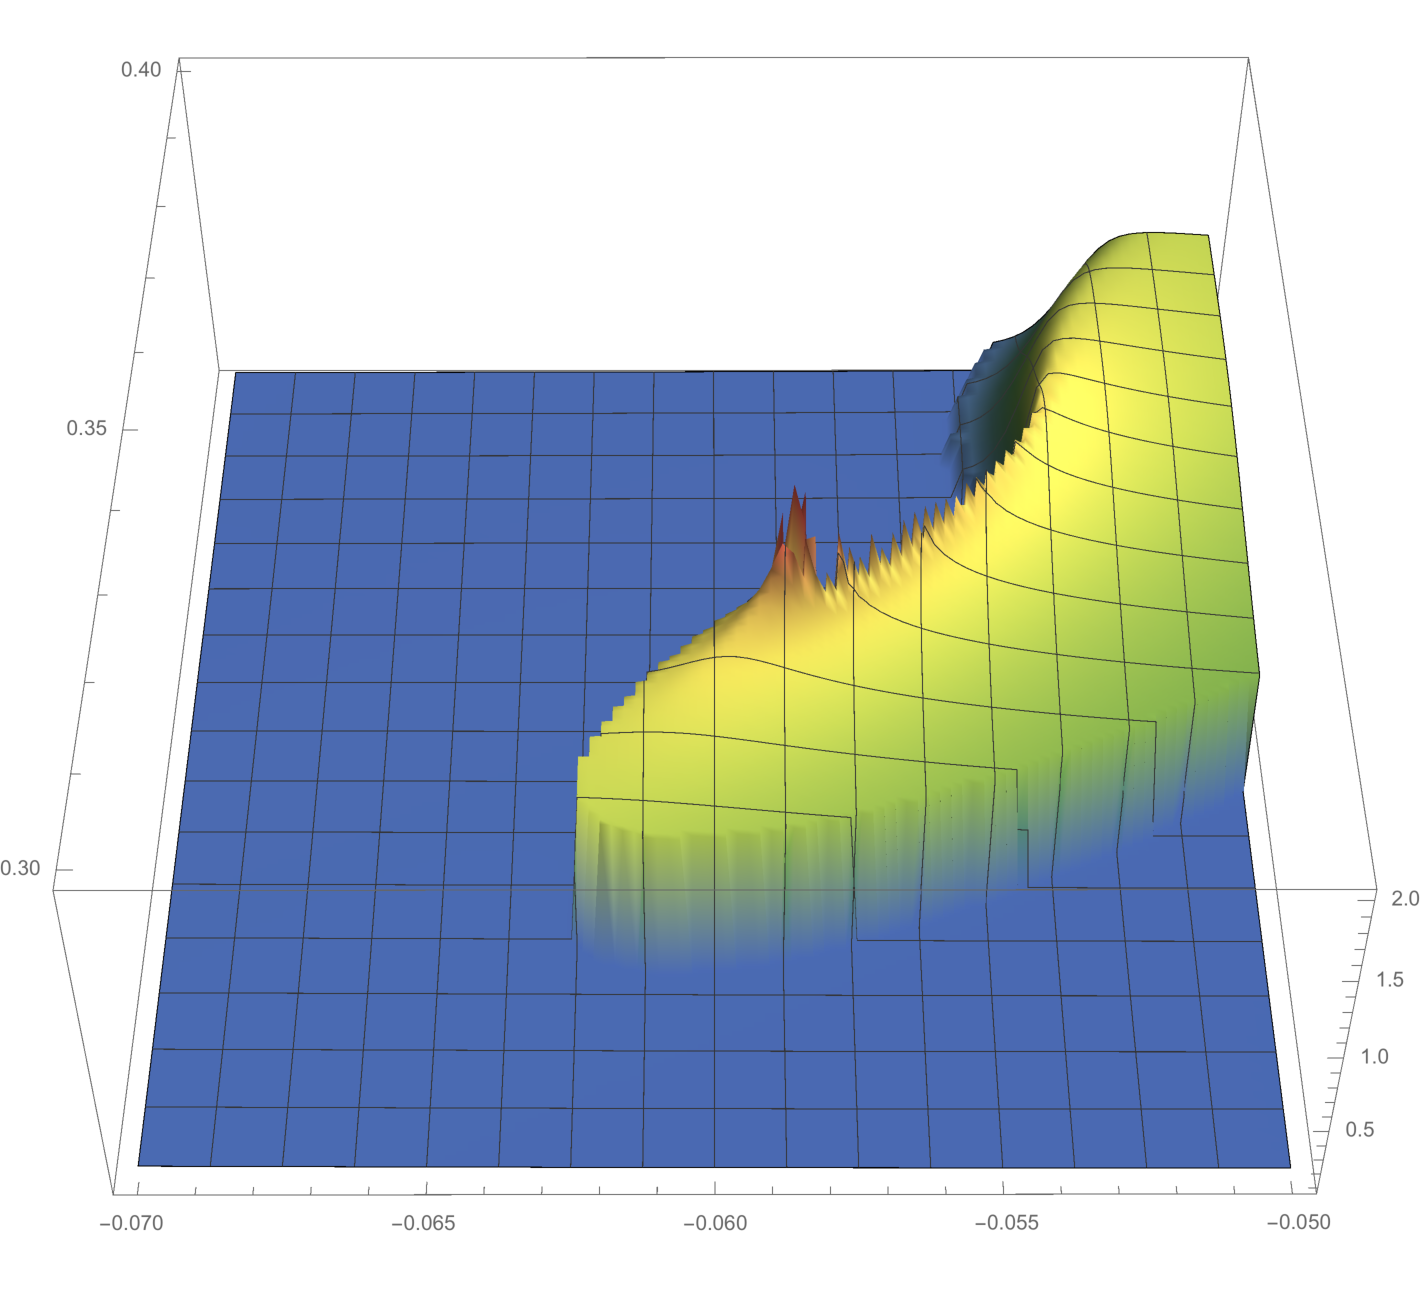
\includegraphics[scale=0.5]{Immagini/spiked3N1.pdf}
\caption{The case $N=1$. The peak is located at $(-0.0585, 0.344)$.}
\label{fig:3}
\end{center}
\end{figure}


\begin{figure}
\begin{center}
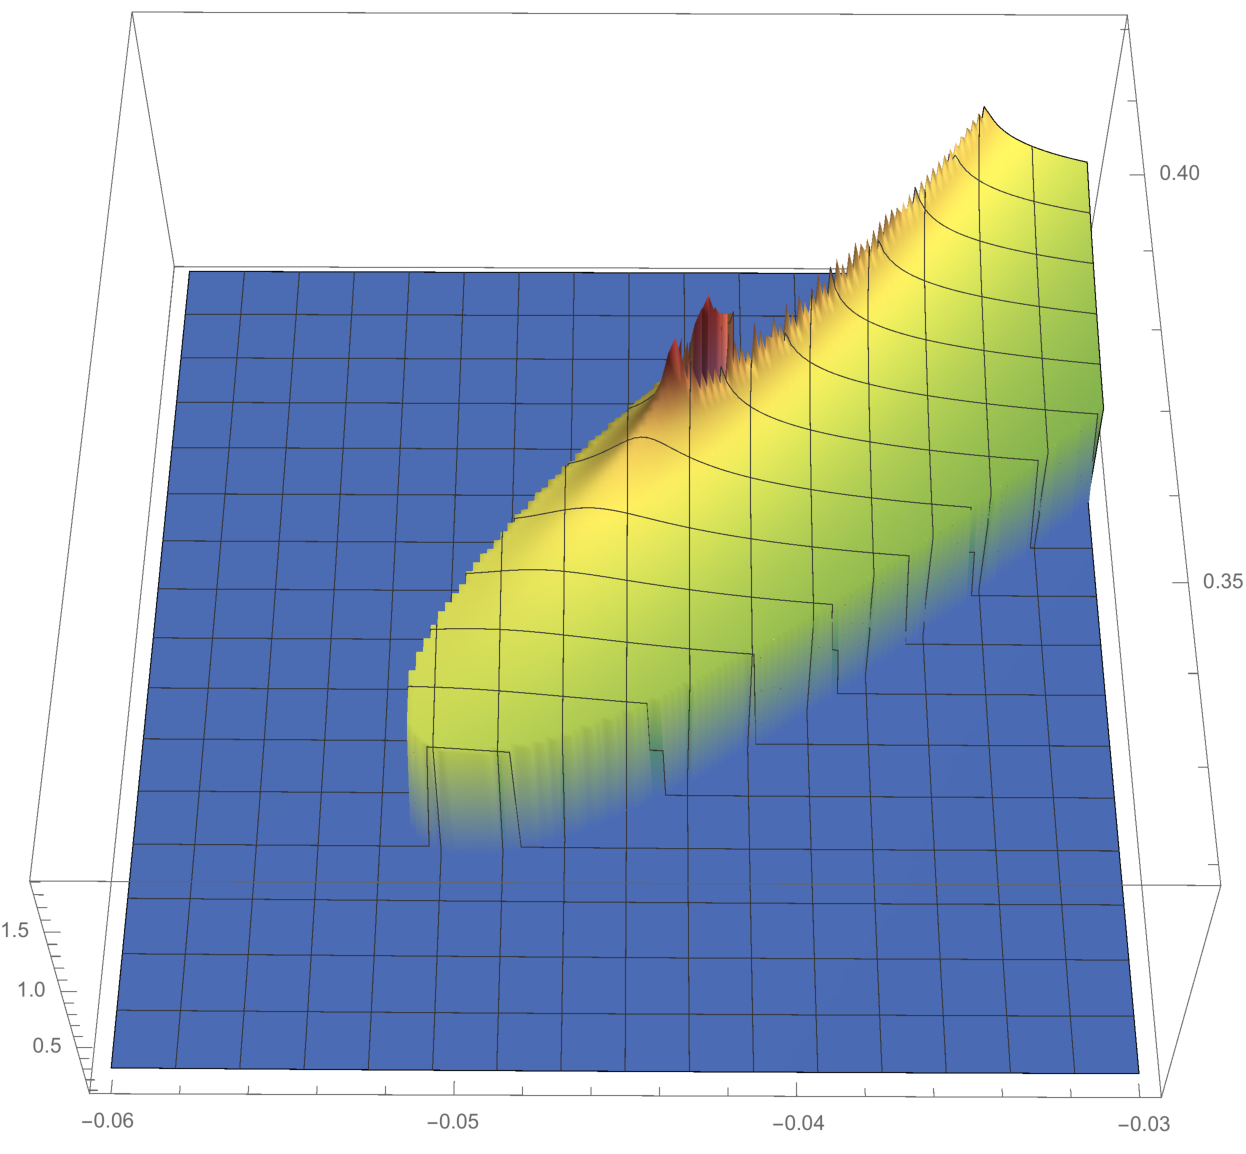
\includegraphics[scale=0.5]{Immagini/spiked3N1p5.pdf}
\caption{Plot of the function $\bar \rho (\sigma_1, \sigma_2)$ for N = 3/2. The peak results to be located at $(-0.0425, 0.385)$}
\label{fig:1}
\end{center}
\end{figure}


\begin{figure}
\begin{center}
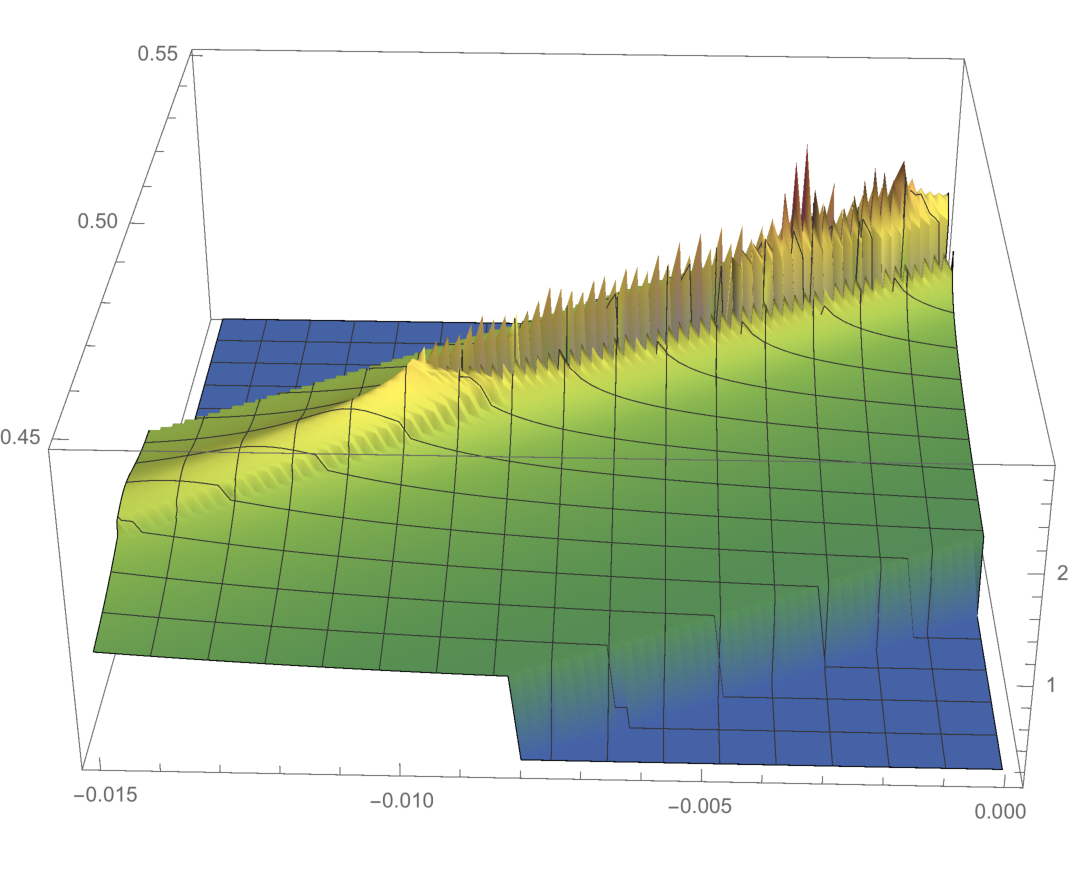
\includegraphics[scale=0.5]{Immagini/spiked3N2front.pdf}
\caption{Plot of the function $\bar \rho (\sigma_1, \sigma_2)$ for N = 2. It looks like there are two peaks, one close to the other.}
\label{fig:2}
\end{center}
\end{figure}


\begin{figure}
\begin{center}
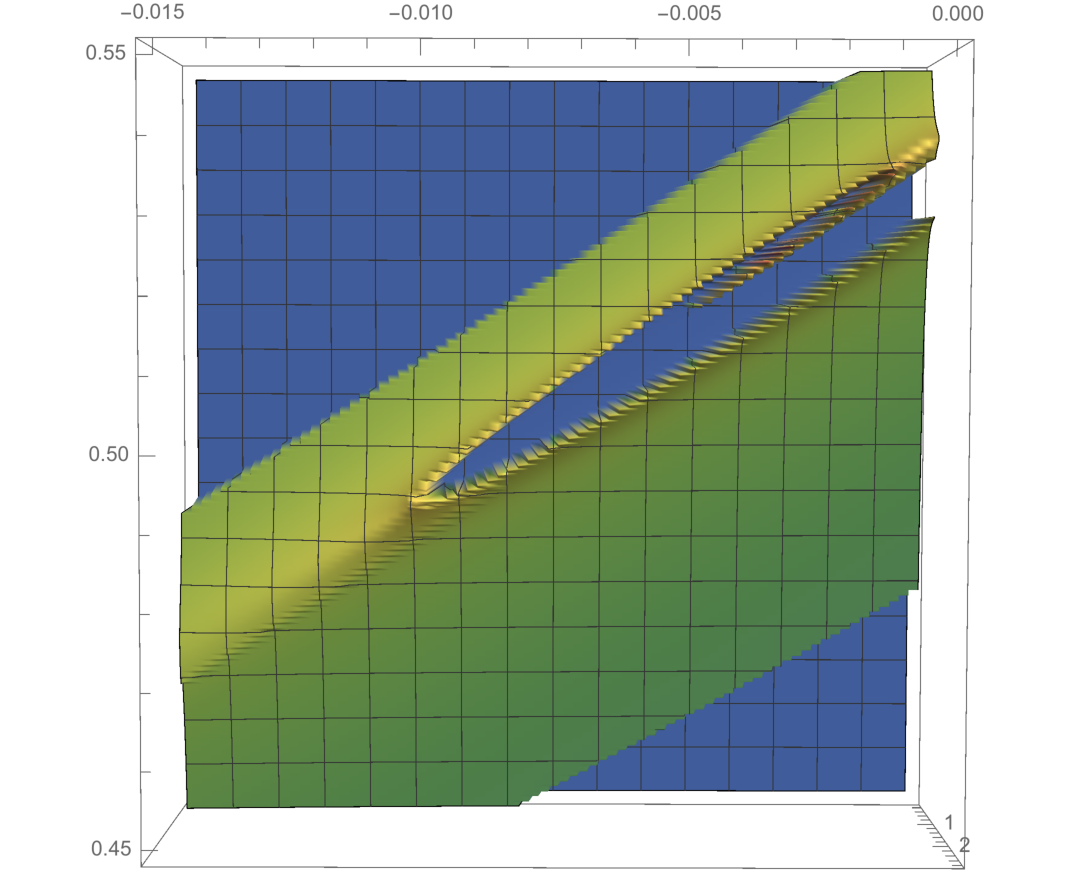
\includegraphics[scale=0.5]{Immagini/spiked3N2top.pdf}
\caption{A top view of the two peaks in the case $N=2$. The highest peak is located at (-0.0029, 0.5260)}
\label{fig:4}
\end{center}
\end{figure}



\begin{figure}
\begin{center}
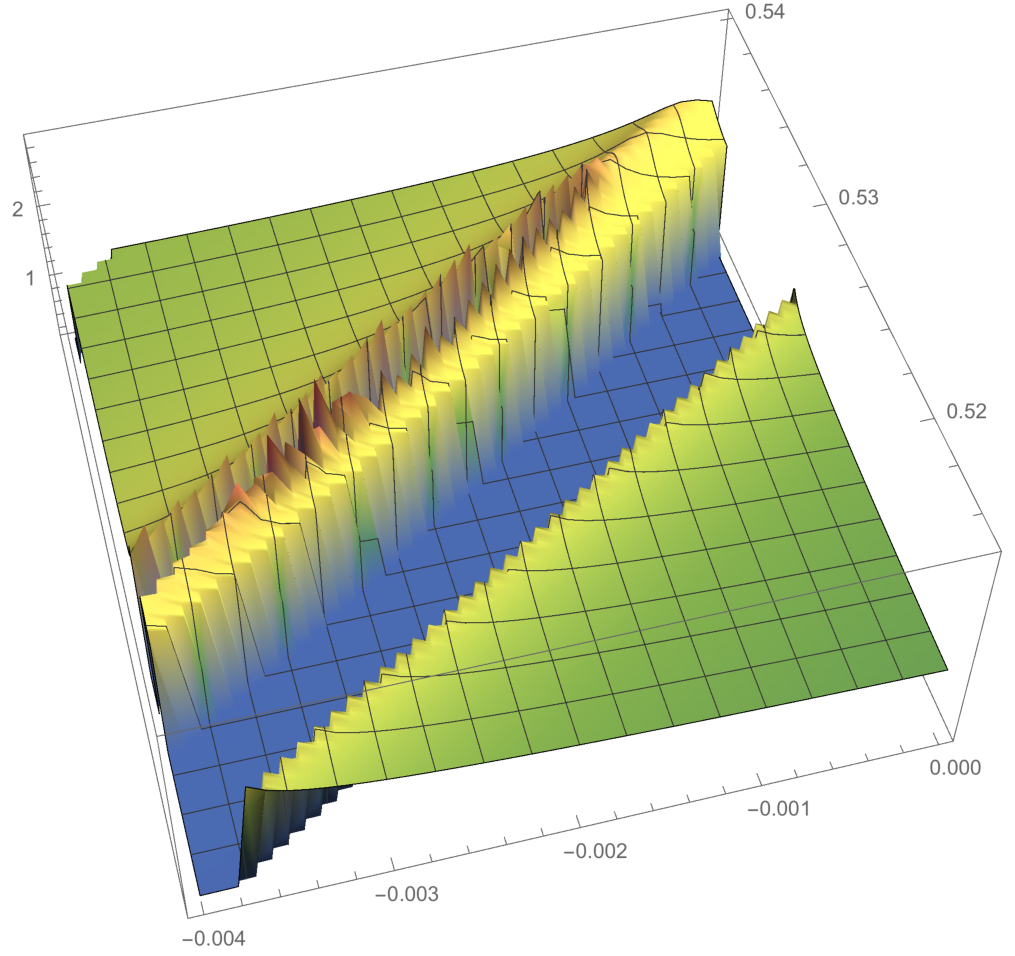
\includegraphics[scale=0.5]{Immagini/spiked3N2-zoomed.pdf}
\caption{A zoom of the region of the domain of $\bar \rho$ where the peaks are located.}
\label{fig:5}
\end{center}
\end{figure}






\newpage 
\subsection{Polynomial Analysis}
A valuable tool can be the analysis of the solutions expanded in power series around the origin or around a non trivial vacuum.
The expansion around the origin in case of a broken phase provides typically a slightly worst description with respect to the second one, which is in general preferable.

In a neighborhood of the origin  the  polynomial expansions of $u(\rho)$ and $f(\rho)$ are:
\begin{equation}
 u(\rho) = \sum _{n=2}^{N_u} \frac{\lambda _n \rho^n}{n!}+\lambda _0
\end{equation}\begin{equation}
 f(\rho) = \sum _{n=0}^{N_f} \frac{f_n \rho^n}{n!}
\end{equation}
and, in the neighborhood of the potential minimum:
\begin{equation}
 u(\rho) = \sum _{n=2}^{N_u} \frac{\lambda _n (\rho -\kappa )^n}{n!}+\lambda _0
\end{equation}\begin{equation}
 f(\rho) = \sum _{n=0}^{N_f} \frac{f_n (\rho -\kappa )^n}{n!}
\end{equation}
Where I have defined $\kappa$ as the value of the dimensionless field modulus square at the minimum of the potential:
\begin{equation}
u'(\kappa) = 0
\end{equation}


Substituting these polynomial expansions of a given order into the fixed point equations and expanding around zero or around the minimum, on obtains a set of algebraic equations whose solutions may give an approximate 
polynomial solution to the differential equation within some bounded region.
Typically one finds many spurious solutions and it is a difficult task to search for a ``good'' one. Nevertheless, if one succeed in this, very often one obtains locally a pretty good approximation of the solution.

We show here an exampe of a polynomial solution obtained with a expansion around a non trivial vacuum for the case $N=1.5$ in Tab.\ref{tab:poli}.

\begin{figure}
\begin{center}
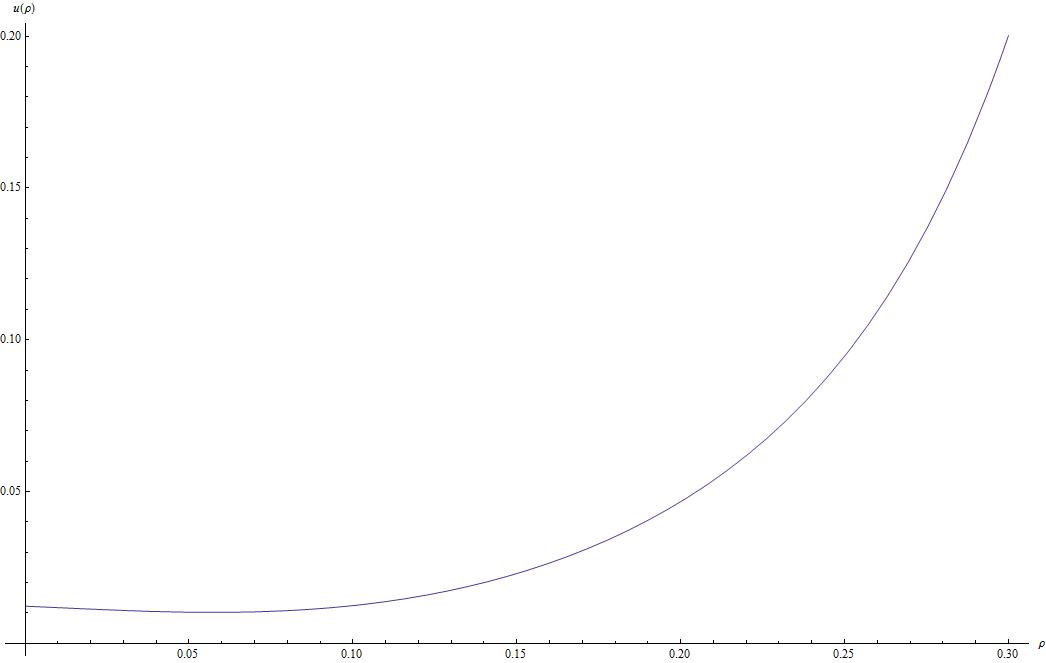
\includegraphics[scale=0.25]{Immagini/plotuN1.jpg}
\caption{Plot of the polynomial expansion around the nontrivial minimum of the dimensionless effective potential $u(\rho)$ for N=3/2.}
\label{fig:plotfN1}
\end{center}
\end{figure}

\begin{table}
  \begin{center}
    \begin{small}
      \begin{tabular}{|c|c|}
 \hline 
 &   \textbf{Results of the polynomial analysis for $N=3/2$, $N_u = 7$ and $N_f = 6$} \\ \hline 
$\lambda_0$ & $0.010174597$  \\ \hline
$\kappa$ & $0.057469286$ \\ \hline 
$\lambda_2$ & $1.9926498$ \\ \hline 
$\lambda_3$ & $34.887704$ \\ \hline 
$\lambda_4$ & $-236.78017$ \\ \hline 
$\lambda_5$ & $8412.4279$ \\ \hline 
$\lambda_6$ &  $-257655.64$ \\ \hline 
$\lambda_7$ &  $9.8750075*10^6$\\ \hline 
$f_0$ & $  0.082295013$ \\ \hline 
$f_1$ & $0.31782706$ \\ \hline 
$f_2$ & $  -0.76423349$ \\ \hline 
$f_3$ & $12.391789$ \\ \hline 
$f_4$ & $-203.83313$ \\ \hline 
$f_5$ & $3149.2212$ \\ \hline 
$f_6$ & $-74077.151$ \\ \hline 

\end{tabular}
    \end{small}
  \end{center}
\caption{Numerically evaluated coefficients $\lambda_i$ and $f_i$ for $N_u = 7$ and $N_f=6$ for the expansion of the potential around the non trivial minimum, in the case $N=3/2$.}
\label{tab:poli}
\end{table}



\begin{figure}
\begin{center}
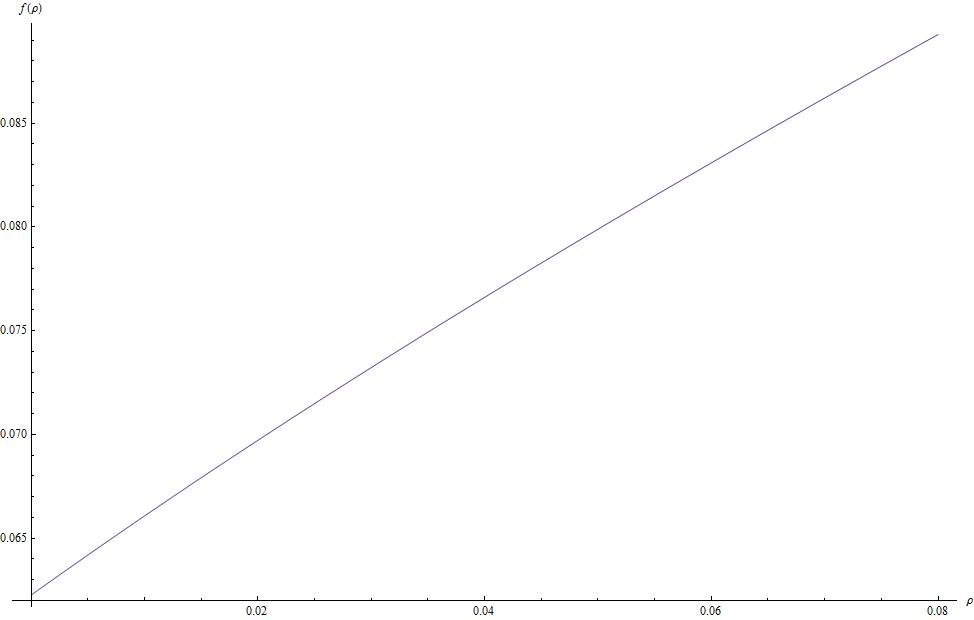
\includegraphics[scale=0.25]{Immagini/plotfN1.jpg}
\caption{Plot of the polynomial expansion of $f(\rho)$  around the non trivial minimum of  the potential for N=3/2.}
\label{fig:plotfN1}
\end{center}
\end{figure}













%%%%%%%%%%%%%%%%%%%%%%%%%%%%%%%%%%%%% FINO A QUI  %%%%%%%%%%%%%%%%%%%%%%%%%%%%%%%%%%%%%%%%%%%%%%%%%%%%%



\renewcommand{\theequation}{\arabic{equation}}%consigliato per migliorare i numeri di equazione nell'introduzione
\renewcommand{\thesection}{\arabic{section}}%consigliato per migliorare i numeri di equazione nell'introduzione
     %%%%%%%%%%%%%%%%%%%%
     %                  %
     %  conclusioni.tex %
     %                  %
     %%%%%%%%%%%%%%%%%%%%
\chapter*{Conclusion}
\noindent

In this thesis I have studied the nonperturbative renormalization group techniques applied to the physics of a scalar linear sigma model,
a quantum field theory whith an internal $O(N)$ symmetry. 
I have considered both the case of a QFT defined on an D dimensional Euclidean flat spacetime and, in three dimensions,
the case of a general non minimal coupling to a gravitational field, which has been treated as a QFT within 
the paradigm of the asymptotic safety.

In the flat spacetime case I have studied the model using an effective average action truncated at the second order in the derivative expansion and I have analytically  derived the flow equation for the relevant quantities 
of the model. Then the special case of $N\to \infty$ has been investigated in order to obtain simplified equations which can be used to investigate the fixed point structure of the model. We distinguish three different cases: 
\begin{enumerate}
 \item Wavefunction renormalization identically constant and vanishing anomalous dimension
 \item Non constant wavefunction renormalization and vanishing anomalous dimension
 \item Non constant wavefunction renormalization and nonvanishing anomalous dimension
\end{enumerate}
The first case has already been studied in the literature, while the other two are investigated for the first time. 
In the case of a vanishing anomalous dimension I was able to give evidence to the conjecture of Morris and Turner \cite{morristurner}, while the study of the most
general case revealed numerically too hard to solve so I had let it for future works, having discussed some of the analytical/numerical tools which should be used to attack and solve the problem in general.

Regarding the case of the scale $O(N)$ model in integration with the gravitational field, I have considered a theory defined on a $3$ dimensional space in which the gravity is treated as a QFT in the 
paradigm of the asymptotic safety. Within a specific formulation of the background field theory of gravity, gauge fixing choice as well as a particular coarse-graining scheme of renormalization, 
previously used in the literature, the flow equations for the effective average action, and in particular for the two ``potentials'' is the LPA truncation, have bee derived.
I stress that with this approach one is able to study the RG flow of a theory with an infinite number of couplings, since an infinite number of them is necessary to descrive the functions $u(\rho)$ 
and $f(\rho)$ in any base of the functional space, where $\rho=\phi^a \phi^a/2$.
Then I looked for the fixed point to the model, deriving analytically two of them as a function of the parameter $N$.
One of this fixed point action is an Einstein-Hilbert action with a cosmological constant and a ``free'' scalar theory, in the sense that it interacts with gravity only through the kinetic term,
but as soon as one deviates from the fixed point the RG flow towards the IR generates in the effective average action several operators. Essentially they correspond, close to the fixed point, to the ones associated to the relevant directions.
The second scaling solution corresponds to a scalar $O(N)$ model with also a non minimal coupling to gravity with the operator of the form $\xi \rho R$. 
Considerations similar to the previous case, when a bare action is located close to the fixed point and one studies the flow towards the IR, can be made.

Then  I have written a numerical routine in order to find other non trivial fixed point. It is based on a shooting method, that needs as input two  parameters $\sigma_1$ and $\sigma_2$, that represents the initial values for the first derivatives 
of $u(\rho)$ and $f(\rho)$, while $u(\rho)$ and $f(\rho)$ are found imposing the fixed point equations to be satisfied.

Then the function $\rho(\sigma_1, \sigma_2)$ has been plotted, looking for its peak,
corresponding to physically acceptable global solutions.

The values of $\sigma_1$ and $\sigma_2$ have then been found for $N=1$, $N=3/2$ and $N=2$:
\begin{enumerate}
 \item $N=1$, $(\sigma_1, \sigma_2) \simeq (-0.0585, 0.344)$;
 \item $N=3/2$, $(\sigma_1, \sigma_2) \simeq (-0.0425, 0.385)$;
 \item $N=2$, $(\sigma_1, \sigma_2) \simeq (-0.0029, 0.5260)$;
\end{enumerate}
The full construction of the global solution is up to now not very accurate, having being match only to local polynomial expansions but to asymtptotic expansions of global numerical solutions covering the asymptotic region.
Moreover pseudo spectral method, discussed in section 4 could reveal themselves to be the best approach to solve globally such a kind of problems. 

These solutions, having the first derivative of the potential in the origin $u'(0)<0$, are in a broken phase.
They can be considered as a deformation of the Wilson-Fisher fixed point which in flat space are, for example, for $N=1$, associated to the Ising universality class, which is induced by the dynamical gravitational interaction.
Such a non trivial solution is not expected to survive in $D=4$ as it is already the case for a flat space-time.
Similar results are being currently obtained in different number of dimensions and in particular in $D=4$ and may have interesting cosmological implications.

I have provided some first results for the scaling solutions, which should be completed by analysing the general dependence in $N$, 
including that in the large N limit which can be probably carried on analytically. Moreover the spectral analysis for the eigenperturbations of the 
linearized equations around the fixed points is necessary to understand the dimension of the UV critical surface and the set of operators which are relevant. 
This latter task requires in general a numerical approach. Of curse finally one should also study the full global flow from the UV to the IR.

These results can be extended in several directions, and the approach should be repeated with other coarse-graining schemes to verify the robustness against it.

\renewcommand{\theequation}{\thechapter.\arabic{equation}}%si torna alle formule numerate come da default
\renewcommand{\thesection}{\thechapter.\arabic{section}}%si torna alle sezioni numerate come da default
\appendix


\index{appendix}

\chapter{Proper Vertices}
\noindent
In this appendix, I will derive the functional derivatives of $\Gamma_k(\phi)$ respect to the field $\phi_i$ up to the fourth order.
For the sake of convenience, I will work with the integrand of the effective action $\gamma(\phi)$, rather than with the effective action itself. 
I will use the following notations:
$$\Gamma_k(\phi) = \int \gamma_k(\phi) d^Dx = \int [ U_k(\rho) + \gamma^Z_k(\phi) +\gamma^Y_k(\phi) ] d^Dx = \int \gamma_k(\phi) d^Dx = \int U_k(\rho) d^Dx  + \Gamma^Z_k(\phi) +\Gamma^Y_k(\phi) $$
where:
\begin{itemize}
 \item $\gamma^Z_k(\phi) = \frac{1}{2}Z_k(\rho) \partial^\mu \phi_i \partial_\mu \phi^i$
 \item $\gamma_k^{Y} = \frac{1}{4} Y_k(\rho) \partial^\mu \rho \partial_\mu \rho =  \frac{1}{4} Y_k(\rho) \phi_i\partial^\mu \phi^i \phi_j\partial_\mu \phi^j$
\end{itemize}
In this thesis I have considered small fluctuation of the fields around a constant backgroung configuration so, at the end of the computation, the value of every observable 
will be calculated for constant fields.
\begin{equation*}
 \phi^i(x) = \bar{\phi}^i + \delta\phi^i(x)
\end{equation*}
and, analogously, in momentum space we have:
\begin{equation*}
 \phi^i(p) = \bar{\phi}^i + \delta\phi^i(p)
\end{equation*}
So the effective average action in momentum space can be expressed as a series expansion of power of $\delta\phi_i$, the coefficients being the proper vertices:
\begin{equation*}
 \Gamma_k(\phi) = \Gamma_k(\bar{\phi}) + \left.\frac{\delta\Gamma_k(\phi)}{\delta\phi_i(p_1)}\right|_{\bar{\phi}}\delta\phi^i(p_1) + \left.\frac{\delta^2\Gamma_k(\phi)}{\delta\phi_i(p_1)\delta\phi_j(p_2)}\right|_{\bar{\phi}}\delta\phi^i(p_1)\delta\phi^j(p_2) +
\end{equation*}
\begin{equation*}
 + \left.\frac{\delta^3\Gamma_k(\phi)}{\delta\phi_i(p_1)\delta\phi_j(p_2)\delta\phi_k(p_3)}\right|_{\bar{\phi}}\delta\phi^i(p_1)\delta\phi^j(p_2)\delta\phi^k(p_3) + \left.\frac{\delta^3\Gamma_k(\phi)}{\delta\phi_i(p_1)\delta\phi_j(p_2)\delta\phi_k(p_3)\delta\phi_l(p_4)}\right|_{\bar{\phi}}\delta\phi^i(p_1)\delta\phi^j(p_2)\delta\phi^k(p_3)\delta\phi^l(p_4)
\end{equation*}

In order to obtain the expressions of $\Gamma_k^{(n)}$  in momentum space, I need to calculate the Fourier transformation of the related direct-space expression.
I will define four tetramomentum vectors $p_1$, $p_2$, $p_3$ and $p_4$, so the proper vertex in momentum space will be defined by the expressions:
\begin{enumerate}
 \item $$\widetilde{\Gamma}^{(2)}_k(p_1, p_2) = \int  d^Dx \int d^Dy_1\int d^Dy_2 \left[\frac{\delta^2 U_k(\rho)}{\delta \phi_a(y_1)\delta \phi_b(y_2)} + \frac{\delta^2 \gamma_k^{Z}}{\delta \phi_a(y_1)\delta \phi_b(y_2)} +\frac{\delta^2 \gamma_k^{Y}}{\delta \phi_a(y_1)\delta \phi_b(y_2)} \right]\e^{-ip_1y_1}\e^{-ip_2y_2}$$
 \item $$\widetilde{\Gamma}^{(3)}_k(p_1, p_2, p_3) =  \int  d^Dx \int d^Dy_1\int d^Dy_2 \int d^Dy_3 \Bigg[\frac{\delta^3 U_k(\rho)}{\delta \phi_a(y_1)\delta \phi_b(y_2)\delta \phi_c(y_3)} + $$  \\ \\ 
       $$ + \frac{\delta^3 \gamma_k^{Z}}{\delta \phi_a(y_1)\delta \phi_b(y_2)\delta \phi_c(y_3)} +\frac{\delta^3 \gamma_k^{Y}}{\delta \phi_a(y_1)\delta \phi_b(y_2)\phi_c(y_3)} \Bigg]\e^{-ip_1y_1}\e^{-ip_2y_2}\e^{-ip_3y_3}$$
 \item $$\widetilde{\Gamma}^{(4)}_k(p_1, p_2, p_3, p_4) = $$ \\ \\ $$ = \int  d^Dx \int d^Dy_1 \int d^Dy_2 \int d^Dy_3\int d^Dy_4 \Big[\frac{\delta^4 U_k(\rho)}{\delta \phi_a(y_1)\delta \phi_b(y_2)\delta \phi_c(y_3)\phi_d(y_4)} + $$\\ $$ +\frac{\delta^4 \gamma_k^{Z}}{\delta \phi_a(y_1)\delta \phi_b(y_2)\delta \phi_c(y_3)\phi_d(y_4)}+\frac{\delta^4 \gamma_k^{Y}}{\delta \phi_a(y_1)\delta \phi_b(y_2)\phi_c(y_3)\phi_d(y_4)} \Bigg]\e^{-ip_1y_1}\e^{-ip_2y_2}\e^{-ip_1y_3}\e^{-ip_4y_4}$$
\end{enumerate}
In order to obtain the Fourier transforms it's necessary to consider the integral representation of the Dirac distribution:
\begin{equation*}
 \delta(x) = \frac{1}{(2\pi)^D}\int \e^{ikx}d^Dx
\end{equation*}
In the following calculations I will use the notations:
\begin{enumerate}
 \item $\mathcal{O}^{(n)}$, with $n$ arabic numeral $ \longrightarrow$  $n^{th}$ functional derivative with respect to the field $\phi$.
 \item $\mathcal{O}^{N}$, with $N$ roman numeral $ \longrightarrow$  $N^{th}$ functional derivative with respect to $\rho = \frac{1}{2}\phi^i\phi_i$
\end{enumerate}

\section{Derivatives of the potential $U_k(\rho)$}
\subsection{I order derivative}
\subsubsection{I order derivative in direct space}
\begin{equation}
 \frac{\delta U_k(\rho)}{\delta \phi_a(y_1)} = U'_k(\rho)\phi^a\delta(x - y_1)
\end{equation}
\subsubsection{I order derivative in momentum space}
\begin{equation}\label{U1}
 \int  \frac{d^Dp_1}{(2\pi)^D} U_k^{(1)}(\rho, p_1) = U'_k(\rho)\phi^a\delta(p_1)
\end{equation}
\subsection{II order derivative}
\subsubsection{II order derivative in direct space}
\begin{equation}
 \frac{\delta^2 U_k(\rho)}{\delta \phi_a(y_1)\delta \phi_b(y_2)} = U'_k(\rho)\delta^{ab}\delta(x - y_1)\delta(y_1 - y_2) + U''_k(\rho)\delta(x-y_1)\delta(x-y_2) {\phi}^a{\phi}^b
\end{equation}
\subsubsection{II order derivative in momentum space}
\begin{equation}\label{U2}
\int  \frac{d^Dp_1}{(2\pi)^D} U_k^{(2)}(\rho, p_1, p_2) = \left[U'_k(\rho)\delta^{ab} + U''_k(\rho){\phi}^a{\phi}^b\right]\delta\left(\sum_{i = 1}^2 p_i \right) 
\end{equation}
\subsection{III order derivative}
\subsubsection{III order derivative in direct space}
\begin{equation}
\frac{\delta^3 U_k(\rho)}{\delta \phi_a(y_1)\delta \phi_b(y_2)\delta \phi_c(y_3)} = 
\end{equation}
$$\delta(x - y_1)\Big\{\big[ \delta(x - y_3) \delta(y_1 - y_2)\delta^{ab}\phi^c(y_3) + \delta(x - y_2)\delta(y_1 - y_3)\delta^{ac}\phi^b(y_2)\ +$$
$$+ \delta(x - y_2)\delta(y_2 - y_3)\delta^{bc}\phi^a(y_1)\big]U_k''(\rho) + \delta(x - y_3)\delta(x-y_2)\phi^a(y_1)\phi^b(y_2)\phi^c(y_3)U_k'''(\rho)\Big\} $$
\subsubsection{III order derivative in momentum space}
\begin{equation}\label{U3}
\int  \frac{d^Dp_1}{(2\pi)^D} U_k^{(3)}(\rho, p_1, p_2, p_3) = \left[\big\{\delta^{ab}\phi^c + \delta^{ac}\phi^b + \delta^{bc}\phi^a\big\}U_k''(\rho) + \phi^a\phi^b\phi^cU_k'''(\rho)\right]\delta\left(\sum_{i=1}^3 p_i\right)
\end{equation}

\subsection{IV order derivative}
\subsubsection{IV order derivative in direct space}
\begin{equation}
\frac{\delta^4 U_k(\rho)}{\delta \phi_a(y_1)\delta \phi_b(y_2)\delta \phi_c(y_3) \phi_d(y_4)} = 
\end{equation}
$$ \delta(x - y_1) \Big\{ \delta(y_1 - y_2) \delta(x - y_3) \delta(y_3 - y_4)\delta^{ab}\delta^{cd}U_k''(\rho) \ + $$
$$+\ \delta(y_1 - y_4) \delta(x - y_2) \delta(y_2 - y_3)\delta^{ad}\delta^{bc}U_k''(\rho) \ + $$
$$+\ \delta(x - y_2)\delta(y_1 - y_3)\delta(y_2 - y_4)\delta^{ac}\delta^{bd}U_k''(\rho) \ + $$
$$+ \delta(y_1 - y_2) \delta(x - y_3) \delta(x - y_4)\delta^{ab} \phi^c(y_3)\phi^d(y_4)U_k'''(\rho) \ +$$
$$+ \delta(x - y_2) \delta(x - y_3) \delta(y_1 - y_4)\delta^{ad}\phi^b(y_2)\phi^c(y_3)U_k'''(\rho) \ + $$
$$+ \delta(x - y_2) \delta(y_1 - y_3) \delta(x - y_4)\delta^{ac}\phi^b(y_3)\phi^d(y_4)U_k'''(\rho) \ + $$
$$+\ \delta(x - y_2)\delta(y_2 - y_3)\delta(x - y_4)\delta^{bc}\phi^a(y_1)\phi^d(y_4)U_k'''(\rho) \ + $$
$$+\ \delta(x - y_2)\delta(x - y_3)\delta(y_2 - y_4)\delta^{bd}\phi^a(y_1)\phi^c(y_3)U_k'''(\rho) \ + $$
$$+\ \delta(x - y_2)\delta(x - y_3)\delta(y_3 - y_4)\delta^{cd}\phi^a(y_1)\phi^b(y_2)U_k'''(\rho) \ + $$
$$+\ \delta(x - y_2)\delta(x - y_3)\delta(y_3 - y_4)\phi^a(y_1)\phi^b(y_2)\phi^c(y_3)\phi^d(y_4)U_k''''(\rho)\Big\} $$

\subsubsection{IV order derivative in momentum space}
\begin{equation}\label{U4}
\int \frac{d^Dp_1}{(2\pi)^D}  U_k^{(4)}(\rho, p_1, p_2, p_3, p_4)  =  \Bigg\{\Big[ \delta^{ab}\delta^{cd} + \delta^{ad}\delta^{bc} + \delta^{ac}\delta^{bd}\Big]U_k''(\rho) +  
\end{equation}
$$\Big[\delta^{ab} \phi^c\phi^d + \delta^{ad}\phi^b\phi^c +\delta^{ac}\phi^b\phi^d +\delta^{bc}\phi^a\phi^d +\delta^{bd}\phi^a\phi^c +\delta^{cd}\phi^a\phi^b\Big]U_k'''(\rho) + $$
$$+\ \phi^a\phi^b\phi^c\phi^dU_k''''(\rho)\Bigg\} \ \delta\left(\sum_{i=1}^4 p_i\right) $$

\section{Derivatives of $\gamma_k^{Z}$}
\subsection{I order derivative}
\subsubsection{I order derivative in direct space}
\begin{equation}
 \left.\frac{\delta \gamma_k^{Z}}{\delta \phi_a(y_1)}\right|_{\bar{\phi}} = \left.\frac{Z'_k(\rho)\phi^a}{2}\delta(x - y_1)\partial^\mu \phi_i \partial_\mu \phi^i + Z_k(\rho)\partial^\mu \phi^a\partial_\mu\delta(x-y_1)\right|_{\bar{\phi}} = 0
\end{equation}
\subsubsection{I order derivative in momentum space}
\begin{equation}\label{Z1}
 \Gamma_Z^{(1)} = 0
\end{equation}
\subsection{II order derivative}
\subsubsection{II order derivative in direct space}
\begin{equation}
 \left. \frac{\delta^2 \gamma_k^{Z}}{\delta \phi_a(y_1)\delta \phi_b(y_2)}\right|_{\bar{\phi}} =
 \end{equation}
$$= \frac{1}{2}Z'_k(\rho)\delta^{ab}\delta(x - y_1)\delta(y_1 - y_2)\partial^\mu \phi_i \partial_\mu \phi^i(x) +  \frac{1}{2}Z''_k(\rho)\delta(x-y_1)\delta(x-y_2){\phi}^a{\phi}^b\partial^\mu \phi_i \partial_\mu \phi^i +$$
$$+Z'_k(\rho)\phi^a\partial^\mu\phi^b\delta(x-y_1)\partial_\mu\delta(x - y_2) + Z_k(\rho)\delta^{ab}\partial^\mu\delta(y_1 - y_2)\partial_\mu\delta(x - y_1) + Z'_k(\rho)\phi^b \partial_\mu\phi^a\partial^\mu\delta(x - y_1)\delta(x - y_2)=$$
$$=Z_k(\rho)\delta^{ab}\partial_\mu\delta(x - y_1)\partial^\mu\delta(y_1 - y_2)$$
\subsubsection{II order derivative in momentum space}
\begin{equation}\label{Z2}
 \Gamma_Z^{(2)} = - Z_k(\rho)\delta^{ab}p_1p_2  \delta\left(\sum_{i=1}^2 p_i\right)
\end{equation}


\subsection{III order derivative}
\subsubsection{III order derivative in direct space}
\begin{equation}
\left. \frac{\delta^3 \gamma_k^{Z}}{\delta \phi_a(y_1)\delta \phi_b(y_2)\delta \phi_c(y_3)}\right|_{\bar{\phi}} = 
\end{equation}
$$\partial_\mu\big(\delta(x-y_2)\big)\delta(x-y_1)\delta(y_1 - y_3)\delta^{ac}\partial_\mu\phi^b(x)Z_k'(\rho)\ + $$
$$+\ \partial_\mu\big(\delta(x-y_3)\big)\delta(x-y_1)\delta(y_1 - y_2)\delta^{ab}\partial_\mu\phi^c(x)Z_k'(\rho)\ + $$
$$+\ \partial_\mu\big(\delta(x-y_1)\big)\delta(x-y_2)\delta(y_3 - y_2)\delta^{bc}\partial_\mu\phi^a(x)Z_k'(\rho)\ + $$
$$+\ \partial_\mu\big(\delta(x-y_2)\big)\partial_\mu\big(\delta(x-y_3)\big)\delta(x - y_1)\delta^{bc}\phi^a(y_1)Z_k'(\rho)\ + $$
$$+\ \partial_\mu\big(\delta(x-y_1)\big)\partial_\mu\big(\delta(x-y_3)\big)\delta(x - y_2)\delta^{ac}\phi^b(y_2)Z_k'(\rho)\ + $$
$$+\ \partial_\mu\big(\delta(x-y_1)\big)\partial_\mu\big(\delta(x-y_2)\big)\delta(x - y_3)\delta^{ab}\phi^c(y_3)Z_k'(\rho)\ + $$
$$+\ \partial_\mu\big(\delta(x-y_3)\big)\delta(x-y_1)\delta(x - y_2)\phi^a(y_1)\phi^b(y_2)\partial_\mu\phi^c(y_3)Z_k''(\rho)\ + $$
$$+\ \partial_\mu\big(\delta(x-y_2)\big)\delta(x-y_1)\delta(x - y_3)\phi^a(y_1)\partial_\mu\phi^b(y_2)\phi^c(y_3)Z_k''(\rho)\ + $$
$$+\ \partial_\mu\big(\delta(x-y_1)\big)\delta(x-y_2)\delta(x - y_3)\partial_\mu\phi^a(y_1)\phi^b(y_2)\phi^c(y_3)Z_k''(\rho)\ + $$
$$+\ \frac{1}{2}\delta(x-y_1)\delta(x-y_2)\delta(y_2 - y_3)\delta^{bc}\phi^a(y_1)\partial_\mu\phi^i(x)\partial^\mu\phi_i(x)Z_k''(\rho)\ + $$
$$+\ \frac{1}{2}\delta(x-y_1)\delta(x-y_2)\delta(x - y_3)\delta^{ac}\phi^b(y_2)\partial_\mu\phi^i(x)\partial^\mu\phi_i(x)Z_k''(\rho)\ + $$
$$+\ \frac{1}{2}\delta(x-y_1)\delta(y_1-y_2)\delta(x - y_3)\delta^{ab}\phi^c(y_3)\partial_\mu\phi^i(x)\partial^\mu\phi_i(x)Z_k''(\rho)\ + $$
$$+\left.\ \frac{1}{2}\delta(x-y_1)\delta(x-y_2)\delta(x - y_3)\phi^a(y_1)\phi^b(y_2)\phi^c(y_3)\partial_\mu\phi^i(x)\partial^\mu\phi_i(x)Z_k'''(\rho)\ \right|_{\bar{\phi}}= $$
$$= \ \ \partial_\mu\big(\delta(x-y_2)\big)\partial_\mu\big(\delta(x-y_3)\big)\delta(x - y_1)\delta^{bc}\phi^a(y_1)Z_k'(\rho)\ + $$
$$+\ \partial_\mu\big(\delta(x-y_1)\big)\partial_\mu\big(\delta(x-y_3)\big)\delta(x - y_2)\delta^{ac}\phi^b(y_2)Z_k'(\rho)\ + $$
$$+\ \partial_\mu\big(\delta(x-y_1)\big)\partial_\mu\big(\delta(x-y_2)\big)\delta(x - y_3)\delta^{ab}\phi^c(y_3)Z_k'(\rho)\ \ $$

\subsubsection{III order derivative in momentum space}
\begin{equation}\label{Z3}
\Gamma_Z^{(3)} = - Z_k'(\rho)\big[p_1p_2\delta^{ab}\phi^c + p_2p_3\delta^{bc}\phi^a + p_3p_1\delta^{ac}\phi^b\big] \delta\left(\sum_{i=1}^3 p_i\right)
\end{equation}


\subsection{IV order derivative}
\subsubsection{IV order derivative in direct space}
\begin{equation}
\left. \frac{\delta^4 \gamma_k^{Z}}{\delta \phi_a(y_1)\delta \phi_b(y_2)\delta \phi_c(y_3)\delta \phi_d(y_4)}\right|_{\bar{\phi}} = 
\end{equation}
$$ \partial^\mu\big(\delta(x - y_1)\big)\partial_\mu\big(\delta(x-y_2)\big)\delta(x - y_3)\delta(y_1 - y_4)\delta^{ab}\delta^{cd} Z_k'(\rho)\ +$$
$$+\ \partial^\mu\big(\delta(x - y_1)\big)\partial_\mu\big(\delta(x-y_2)\big)\delta(x - y_3)\delta(x - y_4)\delta^{ab}\phi^{c}(y_3)\phi^{d}(y_4) Z_k''(\rho)\ +$$
$$+\ \partial^\mu\big(\delta(x - y_1)\big)\partial_\mu\big(\delta(x-y_4)\big)\delta(y_2 - y_3)\delta(x - y_2)\delta^{ad}\delta^{bc} Z_k'(\rho)\ +$$
$$+\ \partial^\mu\big(\delta(x - y_1)\big)\partial_\mu\big(\delta(x-y_4)\big)\delta(x - y_2)\delta(x - y_3)\delta^{ad}\phi^{b}(y_2)\phi^{c}(y_3) Z_k''(\rho)\ +$$
$$+\ \partial^\mu\big(\delta(x - y_1)\big)\partial_\mu\big(\delta(x-y_3)\big)\delta(x - y_2)\delta(y_2 - y_4)\delta^{ac}\delta^{bd} Z_k'(\rho)\ +$$
$$+\ \partial^\mu\big(\delta(x - y_1)\big)\partial_\mu\big(\delta(x-y_3)\big)\delta(x - y_2)\delta(x - y_4)\delta^{ac}\phi^{b}(y_2)\phi^{d}(y_4) Z_k''(\rho)\ +$$
$$+\ \partial^\mu\big(\delta(x - y_1)\big)\delta(x-y_2)\delta(x - y_4)\delta(y_2 - y_3)\delta^{bc}\partial_\mu\phi^{a}(x)\phi^{d}(y_4) Z_k''(\rho)\ +$$
$$+\ \partial^\mu\big(\delta(x - y_1)\big)\delta(x-y_2)\delta(x - y_3)\delta(y_2 - y_4)\delta^{bd}\partial_\mu\phi^{a}(x)\phi^{c}(y_3) Z_k''(\rho)\ +$$
$$+\ \partial^\mu\big(\delta(x - y_1)\big)\delta(x-y_2)\delta(x - y_3)\delta(y_3 - y_4)\delta^{cd}\partial_\mu\phi^{a}(x)\phi^{b}(y_2) Z_k''(\rho)\ +$$
$$+\ \partial^\mu\big(\delta(x - y_1)\big)\delta(x-y_2)\delta(x - y_3)\delta(x - y_4)\delta^{cd}\partial_\mu\phi^{a}(x)\phi^{b}(y_2)\phi^{c}(y_3)\phi^{d}(y_4)Z_k'''(\rho)\ +$$
$$+\ \partial^\mu\big(\delta(x - y_4)\big)\delta(x-y_1)\delta(x - y_3)\delta(y_2 - y_1)\delta^{cd}\partial_\mu\phi^{a}(x)\phi^{b}(y_2) Z_k''(\rho)\ +$$
$$+\ \partial^\mu\big(\delta(x - y_4)\big)\delta(x-y_1)\delta(x - y_3)\delta(y_2 - y_1)\delta^{ab}\partial_\mu\phi^{d}(x)\phi^{c}(y_3) Z_k''(\rho)\ +$$
$$+\ \partial^\mu\big(\delta(x - y_4)\big)\delta(x-y_1)\delta(x - y_2)\delta(y_3 - y_1)\delta^{ac}\partial_\mu\phi^{d}(x)\phi^{b}(y_2) Z_k''(\rho)\ +$$
$$+\ \partial^\mu\big(\delta(x - y_4)\big)\delta(x-y_1)\delta(x - y_2)\delta(y_3 - y_2)\delta^{bc}\partial_\mu\phi^{d}(x)\phi^{a}(y_1) Z_k''(\rho)\ +$$
$$+\ \partial^\mu\big(\delta(x - y_4)\big)\delta(x-y_1)\delta(x - y_2)\delta(x - y_3)\partial_\mu\phi^{d}(x)\phi^{a}(y_1)\phi^{b}(y_2)\phi^{c}(y_3) Z_k'''(\rho)\ +$$
$$+ \partial^\mu\big(\delta(x - y_4)\big)\partial_\mu\big(\delta(x-y_3)\big)\delta(x - y_1)\delta(y_1 - y_2)\delta^{ab}\delta^{cd} Z_k'(\rho)\ +$$
$$+\ \partial^\mu\big(\delta(x - y_3)\big)\partial_\mu\big(\delta(x-y_4)\big)\delta(x - y_1)\delta(x - y_2)\delta^{cd}\phi^{a}(y_1)\phi^{b}(y_2) Z_k''(\rho)\ +$$
$$+\ \partial^\mu\big(\delta(x - y_3)\big)\delta(x-y_1)\delta(x - y_4)\delta(y_1 - y_2)\delta^{ab}\phi^{d}(y_4)\partial_\mu\phi^{c}(x) Z_k''(\rho)\ +$$
$$+\ \partial^\mu\big(\delta(x - y_3)\big)\delta(x-y_1)\delta(y_1 - y_4)\delta(x - y_2)\delta^{ad}\phi^{b}(y_2)\partial_\mu\phi^{c}(x) Z_k''(\rho)\ +$$
$$+\ \partial^\mu\big(\delta(x - y_3)\big)\delta(x-y_1)\delta(y_2 - y_4)\delta(x - y_2)\delta^{bd}\phi^{a}(y_1)\partial_\mu\phi^{c}(x) Z_k''(\rho)\ +$$
$$+\ \partial^\mu\big(\delta(x - y_3)\big)\delta(x-y_1)\delta(x - y_2)\delta(x - y_4)\partial_\mu\phi^{c}(x)\phi^{a}(y_1)\phi^{b}(y_2)\phi^{d}(y_4) Z_k'''(\rho)\ +$$
$$ \partial^\mu\big(\delta(x - y_2)\big)\partial_\mu\big(\delta(x-y_4)\big)\delta(x - y_1)\delta(y_3 - y_1)\delta^{bd}\delta^{ac} Z_k'(\rho)\ +$$
$$+\ \partial^\mu\big(\delta(x - y_2)\big)\partial_\mu\big(\delta(x-y_4)\big)\delta(x - y_3)\delta(x - y_1)\delta^{bd}\phi^{c}(y_3)\phi^{a}(y_1) Z_k''(\rho)\ +$$
$$+ \partial^\mu\big(\delta(x - y_2)\big)\partial_\mu\big(\delta(x-y_3)\big)\delta(x - y_1)\delta(y_4 - y_1)\delta^{bc}\delta^{ad} Z_k'(\rho)\ +$$
$$+\ \partial^\mu\big(\delta(x - y_2)\big)\partial_\mu\big(\delta(x-y_3)\big)\delta(x - y_4)\delta(x - y_1)\delta^{bc}\phi^{d}(y_4)\phi^{a}(y_1) Z_k''(\rho)\ +$$
$$+\ \partial^\mu\big(\delta(x - y_2)\big)\delta(x-y_1)\delta(y_1 - y_3)\delta(x - y_4)\delta^{ac}\phi^{d}(y_4)\partial_\mu\phi^{b}(x) Z_k''(\rho)\ +$$
$$+\ \partial^\mu\big(\delta(x - y_2)\big)\delta(x-y_1)\delta(x - y_3)\delta(x - y_4)\delta^{ad}\phi^{c}(y_3)\partial_\mu\phi^{b}(x) Z_k''(\rho)\ +$$
$$+\ \partial^\mu\big(\delta(x - y_2)\big)\delta(x-y_1)\delta(x - y_3)\delta(y_3 - y_4)\delta^{cd}\phi^{a}(y_1)\partial_\mu\phi^{b}(x) Z_k''(\rho)\ +$$
$$+\ \partial^\mu\big(\delta(x - y_2)\big)\delta(x-y_1)\delta(x - y_3)\delta(x - y_4)\partial_\mu\phi^{b}(x)\phi^{a}(y_1)\phi^{c}(y_3)\phi^{d}(y_4) Z_k'''(\rho)\ +$$
$$+\frac{1}{2} \delta(y_1 - y_2)\delta(x-y_1)\delta(x - y_3)\delta(y_3 - y_4)\delta^{cd}\delta^{ab}\partial_\mu\phi^{i}(x)\partial^\mu\phi_i(x) Z_k''(\rho)\ +$$
$$+\frac{1}{2} \delta(y_1 - y_2)\delta(x-y_1)\delta(x - y_3)\delta(x - y_4)\delta^{ab}\phi^c(y_3)\phi^d(y_4)\partial_\mu\phi^{i}(x)\partial^\mu\phi_i(x) Z_k'''(\rho)\ +$$
$$+\frac{1}{2} \delta(x - y_2)\delta(x-y_1)\delta(y_2 - y_3)\delta(y_1 - y_4)\delta^{bc}\delta^{ad}\partial_\mu\phi^{i}(x)\partial^\mu\phi_i(x) Z_k''(\rho)\ +$$
$$+\frac{1}{2} \delta(x - y_1)\delta(x-y_2)\delta(x - y_3)\delta(y_1 - y_4)\delta^{ad} \partial_\mu\phi^{i}(x)\partial^\mu\phi_i(x)\phi^b(y_2)\phi^c(y_3) Z_k'''(\rho)\ +$$
$$+\frac{1}{2} \delta(x - y_1)\delta(x-y_2)\delta(y_1 - y_3)\delta(y_1 - y_4)\delta^{ac}\delta^{bd}\partial_\mu\phi^{i}(x)\partial^\mu\phi_i(x) Z_k''(\rho)\ +$$
$$+\frac{1}{2} \delta(x - y_1)\delta(x-y_2)\delta(y_1 - y_3)\delta(x - y_4)\delta^{ac} \partial_\mu\phi^{i}(x)\partial^\mu\phi_i(x)\phi^b(y_2)\phi^d(y_4) Z_k'''(\rho)\ +$$
$$+\frac{1}{2} \delta(x - y_1)\delta(x-y_2)\delta(y_2 - y_3)\delta(x - y_4)\delta^{bc} \partial_\mu\phi^{i}(x)\partial^\mu\phi_i(x)\phi^a(y_1)\phi^d(y_4) Z_k'''(\rho)\ +$$
$$+\frac{1}{2} \delta(x - y_1)\delta(x-y_2)\delta(x - y_3)\delta(y_2 - y_4)\delta^{bd} \partial_\mu\phi^{i}(x)\partial^\mu\phi_i(x)\phi^a(y_1)\phi^c(y_3) Z_k'''(\rho)\ +$$
$$+\frac{1}{2} \delta(x - y_1)\delta(x-y_2)\delta(x - y_3)\delta(y_3 - y_4)\delta^{cd} \partial_\mu\phi^{i}(x)\partial^\mu\phi_i(x)\phi^a(y_1)\phi^b(y_2) Z_k'''(\rho)\ +$$
$$+\frac{1}{2} \delta(x - y_1)\delta(x-y_2)\delta(x - y_3)\delta(x - y_4)\partial_\mu\phi^{i}(x)\partial^\mu\phi_i(x)\phi^a(y_1)\phi^b(y_2)\phi^c(y_3)\phi^d(y_4) Z_k''''(\rho)\Big|_{\bar{\phi}} = $$

$$= \partial^\mu\big(\delta(x - y_1)\big)\partial_\mu\big(\delta(x-y_2)\big)\delta(x - y_3)\delta(y_1 - y_4)\delta^{ab}\delta^{cd} Z_k'(\rho)\ +$$
$$+\ \partial^\mu\big(\delta(x - y_1)\big)\partial_\mu\big(\delta(x-y_2)\big)\delta(x - y_3)\delta(x - y_4)\delta^{ab}\phi^{c}(y_3)\phi^{d}(y_4) Z_k''(\rho)\ +$$
$$+\ \partial^\mu\big(\delta(x - y_1)\big)\partial_\mu\big(\delta(x-y_4)\big)\delta(y_2 - y_3)\delta(x - y_2)\delta^{ad}\delta^{bc} Z_k'(\rho)\ +$$
$$+\ \partial^\mu\big(\delta(x - y_1)\big)\partial_\mu\big(\delta(x-y_4)\big)\delta(x - y_2)\delta(x - y_3)\delta^{ad}\phi^{b}(y_2)\phi^{c}(y_3) Z_k''(\rho)\ +$$
$$+\ \partial^\mu\big(\delta(x - y_1)\big)\partial_\mu\big(\delta(x-y_3)\big)\delta(x - y_2)\delta(y_2 - y_4)\delta^{ac}\delta^{bd} Z_k'(\rho)\ +$$
$$+\ \partial^\mu\big(\delta(x - y_1)\big)\partial_\mu\big(\delta(x-y_3)\big)\delta(x - y_2)\delta(x - y_4)\delta^{ac}\phi^{b}(y_2)\phi^{d}(y_4) Z_k''(\rho)\ +$$
$$+ \partial^\mu\big(\delta(x - y_4)\big)\partial_\mu\big(\delta(x-y_3)\big)\delta(x - y_1)\delta(y_1 - y_2)\delta^{ab}\delta^{cd} Z_k'(\rho)\ +$$
$$+\ \partial^\mu\big(\delta(x - y_3)\big)\partial_\mu\big(\delta(x-y_4)\big)\delta(x - y_1)\delta(x - y_2)\delta^{cd}\phi^{a}(y_1)\phi^{b}(y_2) Z_k''(\rho)\ +$$
$$ \partial^\mu\big(\delta(x - y_2)\big)\partial_\mu\big(\delta(x-y_4)\big)\delta(x - y_1)\delta(y_3 - y_1)\delta^{bd}\delta^{ac} Z_k'(\rho)\ +$$
$$+\ \partial^\mu\big(\delta(x - y_2)\big)\partial_\mu\big(\delta(x-y_4)\big)\delta(x - y_3)\delta(x - y_1)\delta^{bd}\phi^{c}(y_3)\phi^{a}(y_1) Z_k''(\rho)\ +$$
$$+ \partial^\mu\big(\delta(x - y_2)\big)\partial_\mu\big(\delta(x-y_3)\big)\delta(x - y_1)\delta(y_4 - y_1)\delta^{bc}\delta^{ad} Z_k'(\rho)\ +$$
$$+\ \partial^\mu\big(\delta(x - y_2)\big)\partial_\mu\big(\delta(x-y_3)\big)\delta(x - y_4)\delta(x - y_1)\delta^{bc}\phi^{d}(y_4)\phi^{a}(y_1) Z_k''(\rho)$$

\subsubsection{IV order derivative in momentum space}
\begin{equation}\label{Z4}
 \Gamma^{(4)}_Z = - \Bigg\{Z'_k(\rho)\Big[\delta^{ab}\delta^{cd}p_1\cdot p_2 + \delta^{ad}\delta^{bc}p_1\cdot p_4 + \delta^{ac}\delta^{bd}p_1\cdot p_3 + \delta^{ab}\delta^{cd}p_3\cdot p_4 + \delta^{bd}\delta^{ac}p_2\cdot p_4 + \delta^{bc}\delta^{ad}p_2\cdot p_3\Big] +
\end{equation}
$$ + Z_k''(\rho) \Big[\delta^{ab}\phi^c\phi^dp_1\cdot p_2 + \delta^{ad}\phi^b\phi^c p_1\cdot p_4+ \delta^{ac}\phi^b\phi^dp_1\cdot p_3 + \delta^{cd}\phi^a\phi^b p_3\cdot p_4 + \delta^{bd}\phi^a\phi^cp_2\cdot p_4 + \delta^{bc}\phi^a\phi^dp_2\cdot p_3\Big]\Bigg\}\delta\left(\sum^4_{i = 1}p_i\right)$$
\section{Derivatives of $\gamma_k^{Y}$}
\subsection{I order derivative}
\subsubsection{I order derivative in direct space}
\begin{equation}
\left.\left.\frac{\delta\gamma_k^{Y}}{\delta \phi_a(y_1)}\right|_{\bar{\phi}}= \frac{Y'_k(\rho)\phi^a}{4} \delta(x - y_1) \partial^\mu \rho \partial_\mu \rho + \frac{Y_k(\rho)}{2}\partial^\mu\rho\big[\delta(x - y_1)\partial_\mu\phi^a(x) + \phi^a(x)\partial_\mu\delta(x - y_1)\big]\right|_{\bar{\phi}} = 0
\end{equation} 
\subsubsection{I order derivative in momentum space}
\begin{equation}\label{Y1}
 \Gamma^{(1)}_Y = 0
\end{equation}
\subsection{II order derivative}
\subsubsection{II order derivative in direct space}
\begin{equation}
\left.\frac{\delta^2 \gamma_k^{Y}}{\delta \phi_a(y_1)\delta \phi_b(y_2)}\right|_{\bar{\phi}}  = 
\end{equation}
$$  \frac{1}{4}\big(Y'_k(\rho)\delta^{ab}\delta(x-y_1)\delta(y_1 - y_2) + 2\rho Y''_k(\rho)\widehat{\phi}^a\widehat{\phi}^b\delta(x - y_1)\delta(x - y_2)\big)\partial^\mu\rho\partial_\mu\rho\ + $$
$$ + \ \frac{Y'_k(\rho)\phi^b}{2}\delta(x - y_2)\partial^\mu\rho\big(\delta(x - y_1)\partial_\mu\phi^a + \phi^a\partial_\mu\delta(x - y_1)\big)\ + $$
$$+ \ \frac{Y_k(\rho)}{2}\partial_\mu \rho \big( \delta(x - y_1) \delta^{ab} \partial^\mu \delta(y_1 - y_2) + \delta^{ab} \delta(y_1 - y_2)\partial_\mu\delta(x - y_2) \big) \ +$$
$$\left. \ + \frac{Y_k(\rho)}{2}\big(\delta(x - y_1) \partial^\mu\phi^a(x) + \phi^a\partial^\mu\delta(x - y_1)\big) \big(\delta(x - y_2) \partial_\mu\phi^b + \phi^b\partial_\mu\delta(x - y_2)\big)\right|_{\phi=cost} =$$
$$\frac{Y_k(\rho)}{2}\phi^a\phi^b \partial^\mu\delta(x - y_1)\partial_\mu\delta(x - y_2)$$

\subsubsection{II order derivative in momentum space} % SEZIONE COMPLETA%
\begin{equation}\label{Y2}
 \Gamma_Y^{(2)} = -\frac{Y_k(\rho)}{2}\phi^a\phi^b p_1p_2 \delta\left(\sum_{i=1}^2 p_i\right)
\end{equation}

\subsection{III order derivative}   % SEZIONE COMPLETA %
\subsubsection*{III order derivative in direct space}  % SEZIONE COMPLETA %
\begin{equation}
\left.\frac{\delta^3 \gamma_k^{Y}}{\delta \phi_a(y_1)\delta \phi_b(y_2)\delta \phi_c(y_3)}\right|_{\bar{\phi}}  = 
\end{equation}
$$\frac{Y_k(\rho)}{2}\partial^\mu\big(\delta(x-y_3)\big)\delta(x - y_1)\delta(x - y_2) \delta^{ac}\partial_\mu\phi^b(x) \ +$$
$$+\ \frac{Y_k(\rho)}{2}\partial^\mu\big(\delta(x-y_1)\big)\delta(x - y_3)\delta(x - y_2) \delta^{ac}\partial_\mu\phi^b(x) \ +$$
$$+\ \frac{Y_k(\rho)}{2}\partial^\mu\big(\delta(x-y_3)\big)\partial_\mu\big(\delta(x - y_2)\big)\delta(x - y_1)\delta^{ac}\phi^b(x) \ +$$
$$+\ \frac{Y_k(\rho)}{2}\partial^\mu\big(\delta(x-y_1)\big)\partial_\mu\big(\delta(x - y_2)\big)\delta(x - y_3)\delta^{ac}\phi^b(x) \ +$$
$$+\ \frac{Y_k(\rho)}{2}\partial^\mu\big(\delta(x-y_2)\big)\delta(x - y_1)\delta(x - y_3) \delta^{ab}\partial_\mu\phi^c(x) \ +$$
$$+\ \frac{Y_k(\rho)}{2}\partial^\mu\big(\delta(x-y_1)\big)\delta(x - y_2)\delta(x - y_3) \delta^{ab}\partial_\mu\phi^c(x) \ +$$
$$+\ \frac{Y'_k(\rho)}{2}\delta(x-y_1)\delta(x - y_2)\delta(x - y_3) \partial^\mu\phi^a(x)\phi^b(x)\partial_\mu\phi^c(x) \ +$$
$$+\ \frac{Y'_k(\rho)}{2}\partial^\mu\big(\delta(x-y_1)\big)\delta(x - y_2)\delta(x - y_3) \phi^a(x)\phi^b(y_2)\partial_\mu\phi^c(x) \ +$$
$$+\ \frac{Y_k(\rho)}{2}\partial^\mu\big(\delta(x-y_3)\big)\partial_\mu\big(\delta(x - y_2)\big)\delta(x - y_3)\delta^{ab}\phi^c(x) \ +$$
$$+\ \frac{Y_k(\rho)}{2}\partial^\mu\big(\delta(x-y_3)\big)\partial_\mu\big(\delta(x - y_1)\big)\delta(x - y_2)\delta^{ab}\phi^c(x) \ +$$
$$+\ \frac{Y'_k(\rho)}{2}\partial^\mu\big(\delta(x-y_3)\big)\delta(x - y_2)\delta(x - y_1)\partial_\mu \phi^a(x)\phi^b(y_2) \phi^c(x) \ +$$
$$+\ \frac{Y'_k(\rho)}{2}\partial^\mu\big(\delta(x-y_3)\big)\partial_\mu\big(\delta(x - y_3)\big)\delta(x - y_2) \phi^a(x)\phi^b(y_2) \phi^c(x) \ +$$
$$+\ \frac{Y_k(\rho)}{2}\delta(x - y_2)\partial^\mu\big(\delta(x-y_3)\big)\delta(x - y_1)\delta^{bc}\partial_\mu\phi^a(x) \ +$$
$$+\ \frac{Y_k(\rho)}{2}\partial^\mu\big(\delta(x-y_1)\big)\partial_\mu\big(\delta(x - y_3)\big)\delta(x - y_2)\delta^{bc}\phi^a(x) \ +$$
$$+\ \frac{Y_k(\rho)}{2}\delta(x - y_1)\partial^\mu\big(\delta(x-y_2)\big)\delta(x - y_3)\delta^{bc}\partial_\mu\phi^a(x) \ +$$
$$+\ \frac{Y_k(\rho)}{2}\partial^\mu\big(\delta(x-y_2)\big)\partial_\mu\big(\delta(x - y_1)\big)\delta(x - y_3)\delta^{bc}\phi^a(x) \ +$$
$$+\ \frac{Y'_k(\rho)}{2}\delta(x-y_1)\delta(x - y_2)\delta(x - y_3) \partial_\mu\phi^a(x)\partial^\mu\phi^b(x)\phi^c(y_3) \ +$$
$$+\ \frac{Y'_k(\rho)}{2}\partial_\mu\big(\delta(x-y_1)\big)\delta(x - y_2)\delta(x - y_3) \phi^a(x)\partial^\mu\phi^b(x)\phi^c(y_3) \ +$$
$$+\ \frac{Y'_k(\rho)}{2}\partial_\mu\big(\delta(x-y_2)\big)\delta(x - y_1)\delta(x - y_3) \partial^\mu\phi^a(x)\phi^b(x)\phi^c(y_3) \ +$$
$$+\ \frac{Y'_k(\rho)}{2}\partial_\mu\big(\delta(x-y_1)\big)\partial^\mu\big(\delta(x - y_2)\big)\delta(x - y_3) \phi^a(x)\phi^b(x)\phi^c(y_3) \ +$$
$$+\ \frac{Y'_k(\rho)}{2}\partial_\mu\rho\delta(x-y_1)\partial^\mu\big(\delta(x - y_2)\big)\delta(x - y_3) \delta^{ab}\phi^c(y_3) \ +$$
$$+\ \frac{Y'_k(\rho)}{2}\partial_\mu\rho\delta(x-y_2)\partial^\mu\big(\delta(x - y_1)\big)\delta(x - y_3) \delta^{ab}\phi^c(y_3) \ +$$
$$+\ \frac{Y'_k(\rho)}{2}\partial_\mu\rho\delta(x-y_2)\partial^\mu\big(\delta(x - y_3)\big)\delta(x - y_1) \delta^{ac}\phi^b(y_2) \ +$$
$$+\ \frac{Y'_k(\rho)}{2}\partial_\mu\rho\delta(x-y_2)\partial^\mu\big(\delta(x - y_1)\big)\delta(x - y_3) \delta^{ac}\phi^b(y_2) \ +$$
$$+\ \frac{Y'_k(\rho)}{2}\partial_\mu\rho\delta(x-y_2)\delta(x - y_1)\delta(x - y_3) \delta^{bc}\partial^\mu\phi^a(x) \ +$$
$$+\ \frac{Y''_k(\rho)}{2}\partial_\mu\rho\delta(x-y_2)\delta(x - y_1)\delta(x - y_3) \partial^\mu\phi^a(x)\phi^b(y_2)\phi^c(y_3) \ +$$
$$+\ \frac{Y'_k(\rho)}{2}\partial_\mu\rho\delta(x-y_2)\partial^\mu\big(\delta(x - y_1)\big)\delta(y_2 - y_3) \delta^{bc}\phi^a(x) \ +$$
$$+\ \frac{Y''_k(\rho)}{2}\partial_\mu\rho\delta(x-y_2)\partial^\mu\big(\delta(x - y_1)\big)\delta(x - y_3) \phi^a(x)\phi^b(y_2)\phi^c(y_3) \ +$$
$$+\ \frac{Y'_k(\rho)}{2}\partial_\mu\rho\delta(x-y_2) \delta(x - y_1)\delta(y_2 - y_3) \delta^{ab}\partial^\mu\phi^c(x) \ +$$
$$+\ \frac{Y'_k(\rho)}{2}\partial_\mu\rho\delta(x-y_1)\partial^\mu\big(\delta(x - y_3)\big)\delta(y_1 - y_2) \delta^{ab}\phi^c(x) \ +$$
$$+\ \frac{Y''_k(\rho)}{2}\partial_\mu\rho\delta(x-y_1)\delta(x - y_3)\delta(x - y_2) \phi^a(y_1)\phi^b(y_2)\partial^\mu\phi^c(x) \ +$$
$$+\ \frac{Y''_k(\rho)}{2}\partial_\mu\rho\delta(x-y_1)\partial^\mu\big(\delta(x - y_3)\big)\delta(x - y_2) \phi^a(y_1)\phi^b(y_2)\phi^c(x) \ +$$
$$+\ \frac{Y'_k(\rho)}{2}\delta(x-y_1)\delta(x - y_3)\partial^\mu\big(\delta(x - y_2)\big) \phi^a(y_1)\phi^b(x)\partial_\mu\phi^c(x) \ +$$
$$+\ \frac{Y'_k(\rho)}{2}\delta(x-y_1)\delta(x - y_2)\partial^\mu\big(\delta(x - y_3)\big) \phi^a(y_1)\partial_\mu\phi^b(x)\phi^c(x) \ +$$
$$+\ \frac{Y'_k(\rho)}{2}\delta(x-y_1)\partial_\mu\big(\delta(x - y_2)\big)\partial^\mu\big(\delta(x - y_3)\big) \phi^a(y_1)\phi^b(x)\phi^c(x) \ +$$
$$+\ \frac{Y'_k(\rho)}{2}\partial_\mu\rho\delta(x-y_1)\partial^\mu\big(\delta(x - y_3)\big)\delta(x - y_2) \delta^{bc}\phi^a(x) \ +$$
$$+\ \frac{Y'_k(\rho)}{2}\partial_\mu\rho\delta(x-y_1)\partial^\mu\big(\delta(x - y_2)\big)\delta(x - y_3) \delta^{bc}\phi^a(x) \ +$$
$$+\ \frac{Y'_k(\rho)}{2}\partial_\mu\rho\delta(x-y_1)\delta(x - y_2)\delta(x - y_3) \delta^{ac}\partial^\mu\phi^b(x) \ +$$
$$+\ \frac{Y'_k(\rho)}{2}\partial_\mu\rho\delta(x-y_1)\partial^\mu\big(\delta(x - y_2)\big)\delta(y_1 - y_3) \delta^{ac}\phi^b(x) \ +$$
$$+\ \frac{Y''_k(\rho)}{2}\partial_\mu\rho\delta(x-y_1)\delta(x - y_2)\delta(x - y_3) \phi^a(y_1) \partial^\mu\phi^b(x)\phi^c(y_3) \ +$$
$$+\ \frac{Y''_k(\rho)}{2}\partial_\mu\rho\delta(x-y_1)\partial^\mu\big(\delta(x - y_2)\big)\delta(x - y_3) \phi^a(y_1)\phi^b(x)\phi^c(y_3) \ +$$
$$+\ \frac{Y''_k(\rho)}{4}\partial_\mu\rho\partial^\mu\rho\delta(x-y_1)\delta(y_1 - y_2)\delta(x - y_3) \delta^{ab}\phi^c(y_3) \ +$$
$$+\ \frac{Y''_k(\rho)}{4}\partial_\mu\rho\partial^\mu\rho\delta(x-y_1)\delta(x - y_2)\delta(y_1 - y_3) \delta^{ac}\phi^b(y_2) \ +$$
$$+\ \frac{Y''_k(\rho)}{4}\partial_\mu\rho\partial^\mu\rho\delta(x-y_1)\delta(x - y_2)\delta(y_2 - y_3) \delta^{bc}\phi^a(y_1) \ +$$
$$+\left. \frac{Y'''_k(\rho)}{4}\partial_\mu\rho\partial^\mu\rho\delta(x-y_1)\delta(x - y_2)\delta(x - y_3) \phi^a(y_1)\phi^b(y_2)\phi^c(y_3)\right|_{\bar{\phi}} =$$



$$ \frac{Y_k(\rho)}{2}\Big[\partial^\mu\big(\delta(x-y_3)\big)\partial_\mu\big(\delta(x - y_2)\big)\delta(x - y_1)\delta^{ac}\phi^b(x) \ +$$
$$+\ \partial^\mu\big(\delta(x-y_1)\big)\partial_\mu\big(\delta(x - y_2)\big)\delta(x - y_3)\delta^{ac}\phi^b(x) \ +$$
$$+\ \partial^\mu\big(\delta(x-y_1)\big)\partial_\mu\big(\delta(x - y_2)\big)\delta(x - y_3)\delta^{ab}\phi^c(x) \ +$$
$$+\ \partial^\mu\big(\delta(x-y_3)\big)\partial_\mu\big(\delta(x - y_1)\big)\delta(x - y_2)\delta^{ab}\phi^c(x) \ +$$
$$+\ \partial^\mu\big(\delta(x-y_2)\big)\partial_\mu\big(\delta(x - y_1)\big)\delta(x - y_3)\delta^{bc}\phi^a(x) \ +$$
$$+\ \partial^\mu\big(\delta(x-y_2)\big)\partial_\mu\big(\delta(x - y_1)\big)\delta(x - y_3)\delta^{bc}\phi^a(x)\Big] \ +$$
$$+\ \frac{Y'_k(\rho)}{2}\Big[\partial_\mu\big(\delta(x-y_1)\big)\partial^\mu\big(\delta(x - y_2)\big)\delta(x - y_3) \phi^a(x)\phi^b(x)\phi^c(y_3) \ +$$
$$\ \ \ +\ \partial^\mu\big(\delta(x-y_3)\big)\partial_\mu\big(\delta(x - y_3)\big)\delta(x - y_2) \phi^a(x)\phi^b(y_2) \phi^c(x) \ +$$
$$\ \ \ +\ \partial_\mu\big(\delta(x - y_2)\big)\partial^\mu\big(\delta(x - y_3)\big) \delta(x-y_1)\phi^a(y_1)\phi^b(x)\phi^c(x)\Big]$$



\subsubsection{III order derivative in momentum space} % SEZIONE COMPLETA %
\begin{equation}\label{Y3}
 {\Gamma_Y}^{(3)}(p_1, p_2, p_3) =  
\end{equation}
$$ - \left\{Y_k(\rho)\Big[p_1p_2\phi^c\delta^{ab} + p_2 p_3 \phi^a \delta^{bc} + p_3p_1\phi^b\delta^{ca}\Big] + \frac{Y'_k(\rho)}{2}\Big[p_1p_2 + p_2p_3 + p_3p_1\Big]\phi^a\phi^b\phi^c\right\}\delta\left(\sum_{i = 1}^3 p_i \right)$$



\subsection{IV order derivative}

\subsubsection{IV order derivative in direct space}

\begin{equation}
 \left.\frac{\delta^4 \gamma_Y}{\delta\phi^a(y_1)\delta\phi^b(y_2)\delta\phi^c(y_3)\delta\phi^(y_4)}\right|_{\bar{\phi}} = 
\end{equation}
$$ \frac{Y_k(\rho)}{2}\partial^\mu\big(\delta(x - y_4)\big)\partial_\mu\big(\delta(x - y_2)\big)\delta(x - y_1)\delta(x - y_3) \delta^{ab}\delta^{cd}\ +$$
$$+\ \frac{Y_k(\rho)}{2}\partial^\mu\big(\delta(x - y_3)\big)\partial_\mu\big(\delta(x - y_2)\big)\delta(x - y_1)\delta(x - y_4)\delta^{ab}\delta^{cd} \ +$$
$$+\ \frac{Y_k(\rho)}{2}\partial^\mu\big(\delta(x - y_4)\big)\partial_\mu\big(\delta(x - y_1)\big)\delta(x - y_3)\delta(x - y_2)\delta^{ab}\delta^{cd} \ +$$
$$+\ \frac{Y_k(\rho)}{2}\partial^\mu\big(\delta(x - y_3)\big)\partial_\mu\big(\delta(x - y_1)\big)\delta(x - y_4)\delta(x - y_2)\delta^{ab}\delta^{cd} \ +$$
$$+\ \frac{Y'_k(\rho)}{2}\partial^\mu\big(\delta(x - y_4)\big)\delta(x - y_3)\delta(x - y_1)\delta(x - y_2)\partial_\mu\phi^a(x)\phi^b(y_2)\delta^{cd} \ +$$
$$+\ \frac{Y'_k(\rho)}{2}\partial^\mu\big(\delta(x - y_3)\big)\delta(x - y_1)\delta(x - y_4)\delta(x - y_2)\partial_\mu\phi^a(x)\phi^b(y_2)\delta^{cd} \ +$$
$$+\ \frac{Y'_k(\rho)}{2}\partial^\mu\big(\delta(x - y_4)\big)\delta(x - y_3)\partial_\mu\big(\delta(x - y_1)\big)\delta(x - y_2)\phi^a(x)\phi^b(y_2)\delta^{cd} \ +$$
$$+\ \frac{Y'_k(\rho)}{2}\partial^\mu\big(\delta(x - y_3)\big)\delta(x - y_4)\partial_\mu\big(\delta(x - y_1)\big)\delta(x - y_2)\phi^a(x)\phi^b(y_2)\delta^{cd} \ +$$
$$+\ \frac{Y_k(\rho)}{2}\partial^\mu\big(\delta(x - y_4)\big)\partial_\mu\big(\delta(x - y_3)\big)\delta(x - y_2)\delta(x - y_1) \delta^{ad}\delta^{bc}\ +$$
$$+\ \frac{Y_k(\rho)}{2}\partial^\mu\big(\delta(x - y_1)\big)\partial_\mu\big(\delta(x - y_3)\big)\delta(x - y_2)\delta(x - y_4) \delta^{ad}\delta^{bc}\ +$$
$$+\ \frac{Y_k(\rho)}{2}\partial^\mu\big(\delta(x - y_2)\big)\partial_\mu\big(\delta(x - y_4)\big)\delta(x - y_1)\delta(x - y_3) \delta^{ad}\delta^{bc}\ +$$
$$+\ \frac{Y_k(\rho)}{2}\partial^\mu\big(\delta(x - y_1)\big)\partial_\mu\big(\delta(x - y_2)\big)\delta(x - y_3)\delta(x - y_4) \delta^{ad}\delta^{bc}\ +$$
$$+\ \frac{Y'_k(\rho)}{2}\partial^\mu\big(\delta(x - y_4)\big)\delta(x - y_3)\delta(x - y_1)\delta(x - y_2)\partial_\mu\phi^b(x)\phi^c(y_3)\delta^{ad} \ +$$
$$+\ \frac{Y'_k(\rho)}{2}\partial^\mu\big(\delta(x - y_1)\big)\delta(x - y_3)\delta(x - y_4)\delta(x - y_2)\partial_\mu\phi^b(x)\phi^c(y_3)\delta^{ad} \ +$$
$$+\ \frac{Y'_k(\rho)}{2}\partial^\mu\big(\delta(x - y_4)\big)\delta(x - y_1)\partial_\mu\big(\delta(x - y_2)\big)\delta(x - y_3)\phi^b(x)\phi^c(y_3)\delta^{ad} \ +$$
$$+\ \frac{Y'_k(\rho)}{2}\partial^\mu\big(\delta(x - y_1)\big)\delta(x - y_4)\partial_\mu\big(\delta(x - y_2)\big)\delta(x - y_3)\phi^b(x)\phi^c(y_3)\delta^{ad} \ +$$
$$+\ \frac{Y_k(\rho)}{2}\partial^\mu\big(\delta(x - y_3)\big)\delta(x - y_1)\partial_\mu\big(\delta(x - y_4)\big)\delta(x - y_2)\delta^{ac}\delta^{bd} \ +$$
$$+\ \frac{Y_k(\rho)}{2}\partial^\mu\big(\delta(x - y_1)\big)\delta(x - y_3)\partial_\mu\big(\delta(x - y_4)\big)\delta(x - y_2)\delta^{ac}\delta^{bd} \ +$$
$$+\ \frac{Y_k(\rho)}{2}\partial^\mu\big(\delta(x - y_3)\big)\delta(x - y_1)\partial_\mu\big(\delta(x - y_2)\big)\delta(x - y_4)\delta^{ac}\delta^{bd} \ +$$
$$+\ \frac{Y_k(\rho)}{2}\partial^\mu\big(\delta(x - y_1)\big)\delta(x - y_3)\partial_\mu\big(\delta(x - y_2)\big)\delta(x - y_4)\delta^{ac}\delta^{bd} \ +$$
$$+\ \frac{Y'_k(\rho)}{2}\partial^\mu\big(\delta(x - y_3)\big)\delta(x - y_1)\delta(x - y_4)\delta(x - y_2)\partial_\mu\phi^b(x)\phi^d(y_4)\delta^{ac} \ +$$
$$+\ \frac{Y'_k(\rho)}{2}\partial^\mu\big(\delta(x - y_1)\big)\delta(x - y_3)\delta(x - y_4)\delta(x - y_2)\partial_\mu\phi^b(x)\phi^d(y_4)\delta^{ac} \ +$$
$$+\ \frac{Y'_k(\rho)}{2}\partial^\mu\big(\delta(x - y_3)\big)\delta(x - y_1)\partial_\mu\big(\delta(x - y_2)\big)\delta(x - y_4)\phi^b(x)\phi^d(y_4)\delta^{ac} \ +$$
$$+\ \frac{Y'_k(\rho)}{2}\partial^\mu\big(\delta(x - y_1)\big)\delta(x - y_3)\partial_\mu\big(\delta(x - y_2)\big)\delta(x - y_4)\phi^b(x)\phi^d(y_4)\delta^{ac} \ +$$
$$+\ \frac{Y'_k(\rho)}{2}\partial^\mu\big(\delta(x - y_2)\big)\delta(x - y_3)\delta(x - y_1)\delta(x - y_4)\partial_\mu\phi^d(x)\phi^c(y_3)\delta^{ab} \ +$$
$$+\ \frac{Y'_k(\rho)}{2}\partial^\mu\big(\delta(x - y_4)\big)\delta(x - y_3)\partial_\mu\big(\delta(x - y_2)\big)\delta(x - y_1)\phi^c(y_3)\phi^d(x)\delta^{ab} \ +$$
$$+\ \frac{Y'_k(\rho)}{2}\partial^\mu\big(\delta(x - y_1)\big)\delta(x - y_3)\delta(x - y_2)\delta(x - y_4)\partial_\mu\phi^d(x)\phi^c(y_3)\delta^{ab} \ +$$
$$+\ \frac{Y'_k(\rho)}{2}\partial^\mu\big(\delta(x - y_4)\big)\delta(x - y_3)\partial_\mu\big(\delta(x - y_1)\big)\delta(x - y_2)\phi^c(y_3)\phi^d(x)\delta^{ab} \ +$$
$$+\ \frac{Y'_k(\rho)}{2}\partial^\mu\big(\delta(x - y_3)\big)\delta(x - y_1)\delta(x - y_2)\delta(x - y_4)\partial_\mu\phi^d(x)\phi^b(y_2)\delta^{ac} \ +$$
$$+\ \frac{Y'_k(\rho)}{2}\partial^\mu\big(\delta(x - y_4)\big)\delta(x - y_1)\partial_\mu\big(\delta(x - y_3)\big)\delta(x - y_2)\phi^b(y_2)\phi^d(x)\delta^{ac} \ +$$
$$+\ \frac{Y'_k(\rho)}{2}\delta(x - y_4)\delta(x - y_3)\partial_\mu\big(\delta(x - y_1)\big)\delta(x - y_2)\phi^b(y_2)\partial^\mu\phi^d(x)\delta^{ac} \ +$$
$$+\ \frac{Y'_k(\rho)}{2}\partial^\mu\big(\delta(x - y_4)\big)\delta(x - y_3)\partial_\mu\big(\delta(x - y_1)\big)\delta(x - y_2)\phi^b(y_2)\phi^d(x)\delta^{ac} \ +$$
$$+\ \frac{Y'_k(\rho)}{2}\delta(x - y_4)\delta(y_2 - y_3)\delta(x - y_1)\delta(x - y_2)\partial_\mu\phi^a(x)\partial^\mu\phi^d(x)\delta^{bc} \ +$$
$$+\ \frac{Y'_k(\rho)}{2}\partial^\mu\big(\delta(x - y_4)\big)\delta(y_2 - y_3)\delta(x - y_1)\delta(x - y_2)\partial_\mu\phi^a(x)\phi^d(x)\delta^{bc} \ +$$
$$+\ \frac{Y''_k(\rho)}{2}\delta(x - y_4)\delta(y_2 - y_3)\delta(x - y_1)\delta(x - y_2)\partial_\mu\phi^a(x)\partial^\mu\phi^d(x)\phi^b(y_2)\phi^c(y_3) \ +$$
$$+\ \frac{Y''_k(\rho)}{2}\partial^\mu\big(\delta(x - y_4)\big)\delta(x - y_3)\delta(x - y_1)\delta(x - y_2)\partial_\mu\phi^a(x)\phi^d(x)\phi^b(y_2)\phi^c(y_3) \ +$$
$$+\ \frac{Y'_k(\rho)}{2}\delta(x - y_4)\delta(y_2 - y_3)\partial_\mu\big(\delta(x - y_1)\big)\delta(x - y_2)\phi^a(x)\partial^\mu\phi^d(x)\delta^{bc} \ +$$
$$+\ \frac{Y'_k(\rho)}{2}\partial^\mu\big(\delta(x - y_4)\big)\delta(y_2 - y_3)\partial_\mu\big(\delta(x - y_1)\big)\delta(x - y_2)\phi^a(x)\phi^d(x)\delta^{bc} \ +$$
$$+\ \frac{Y''_k(\rho)}{2}\delta(x - y_4)\delta(x - y_3)\partial_\mu\big(\delta(x - y_1)\big)\delta(x - y_2)\phi^a(x)\partial^\mu\phi^d(x)\phi^b(y_2)\phi^c(y_3) \ +$$
$$+\ \frac{Y''_k(\rho)}{2}\partial^\mu\big(\delta(x - y_4)\big)\delta(x - y_3)\partial_\mu\big(\delta(x - y_1)\big)\delta(x - y_2)\phi^a(x)\phi^d(x)\phi^b(y_2)\phi^c(y_3) \ +$$
$$+\ \frac{Y'_k(\rho)}{2}\delta(x - y_3)\delta(x - y_4)\partial_\mu\big(\delta(x - y_2)\big)\delta(x - y_1)\delta^{ab}\partial^\mu\phi^c(x)\phi^d(y_4) \ +$$
$$+\ \frac{Y'_k(\rho)}{2}\delta(x - y_3)\delta(x - y_4)\partial_\mu\big(\delta(x - y_2)\big)\delta(x - y_1)\delta^{ab}\partial^\mu\phi^c(x)\phi^d(y_4) \ +$$
$$+ \frac{1}{2}\partial^\mu\big(\delta(x - y_3)\big)\partial_\mu\big(\delta(x - y_2)\big)\delta(x - y_1)\delta(x- y_4)\delta^{ab}\phi^c(x)\phi^d(y_4)Y'_k(\rho) + $$
$$+ \frac{1}{2}\delta(x - y_3)\partial_\mu\big(\delta(x - y_1)\big)\delta(x - y_2)\delta(x- y_4)\delta^{ab}\partial^\mu\phi^c(x)\phi^d(y_4)Y'_k(\rho) + $$
$$+ \frac{1}{2}\partial^\mu\big(\delta(x - y_3)\big)\partial_\mu\big(\delta(x - y_1)\big)\delta(x - y_2)\delta(x- y_4)\delta^{ab}\phi^c(x)\phi^d(y_4)Y'_k(\rho) + $$
$$+ \frac{1}{2}\delta(x - y_3)\partial_\mu\big(\delta(x - y_4)\big)\delta(x - y_2)\delta(x- y_1)\delta^{ad}\partial^\mu\phi^c(x)\phi^b(y_2)Y'_k(\rho) + $$
$$+ \frac{1}{2}\partial^\mu\big(\delta(x - y_3)\big)\partial_\mu\big(\delta(x - y_4)\big)\delta(x - y_2)\delta(x- y_1)\delta^{ad}\phi^c(x)\phi^b(y_2)Y'_k(\rho) + $$
$$+ \frac{1}{2}\delta(x - y_3)\partial_\mu\big(\delta(x - y_1)\big)\delta(x - y_2)\delta(x- y_4)\delta^{ad}\partial^\mu\phi^c(x)\phi^b(y_2)Y'_k(\rho) + $$
$$+ \frac{1}{2}\partial^\mu\big(\delta(x - y_3)\big)\partial_\mu\big(\delta(x - y_1)\big)\delta(x - y_2)\delta(x- y_4)\delta^{ad}\phi^c(x)\phi^b(y_2)Y'_k(\rho) + $$
$$+ \frac{1}{2}\delta(x - y_3)\delta(x - y_1)\delta(x - y_2)\delta(y_2- y_4)\delta^{bd}\partial^\mu\phi^c(x)\partial_\mu\phi^a(x)Y'_k(\rho) + $$
$$+ \frac{1}{2}\partial^\mu\big(\delta(x - y_3)\big)\delta(x - y_1)\delta(x - y_2)\delta(y_2- y_4)\delta^{bd}\phi^c(x)\partial_\mu\phi^a(x)Y'_k(\rho) + $$
$$+ \frac{1}{2}\delta(x - y_3)\delta(x - y_1)\delta(x - y_2)\delta(x- y_4)\delta^{bd}\phi^b(y_2)\phi^d(y_4)\partial^\mu\phi^c(x)\partial_\mu\phi^a(x)Y''_k(\rho) + $$
$$+ \frac{1}{2}\partial_\mu\big(\delta(x - y_3)\big)\delta(x - y_1)\delta(x - y_2)\delta(x- y_4)\phi^b(y_2)\phi^d(y_4)\phi^c(x)\partial_\mu\phi^a(x)Y''_k(\rho) + $$
$$+ \frac{1}{2}\delta(x - y_3)\partial_\mu\big(\delta(x - y_1)\big)\delta(x - y_2)\delta(y_2 - y_4)\delta^{bd}\partial^\mu\phi^c(x)\phi^a(x)Y'_k(\rho) + $$
$$+ \frac{1}{2}\partial_\mu\big(\delta(x - y_3)\big)\delta(x - y_1)\delta(x - y_2)\delta(x- y_4)\phi^b(y_2)\phi^d(y_4)\phi^c(x)\partial_\mu\phi^a(x)Y'_k(\rho) + $$
$$+ \frac{1}{2}\partial^\mu\big(\delta(x - y_3)\big)\partial_\mu\big(\delta(x - y_1)\big)\delta(x - y_2)\delta(y_2- y_4)\delta^{bd}\phi^c(x)\phi^a(x)Y'_k(\rho) + $$
$$+\ \frac{Y''_k(\rho)}{2}\delta(x - y_3)\partial^\mu\big(\delta(x - y_1)\big)\delta(x - y_2)\delta(x - y_4)\phi^a(x)\partial_\mu\phi^c(x)\phi^b(y_2)\phi^d(y_4) \ +$$
$$+\ \frac{Y''_k(\rho)}{2}\partial_\mu\big(\delta(x - y_3)\big)\partial^\mu\big(\delta(x - y_1)\big)\delta(x - y_2)\delta(x - y_4)\phi^a(x)\phi^c(x)\phi^b(y_2)\phi^d(y_4) \ +$$
$$+\ \frac{Y'_k(\rho)}{2}\delta(x - y_1)\partial^\mu\big(\delta(x - y_3)\big)\delta(x - y_2)\delta(x - y_4)\partial_\mu\phi^a(x)\phi^d(y_4)\delta^{bc} \ +$$
$$+\ \frac{Y'_k(\rho)}{2}\partial_\mu\big(\delta(x - y_3)\big)\partial^\mu\big(\delta(x - y_1)\big)\delta(x - y_2)\delta(x - y_4)\phi^a(x)\phi^d(y_4)\delta^{bc} \ +$$
$$+\ \frac{Y'_k(\rho)}{2}\delta(x - y_1)\partial^\mu\big(\delta(x - y_2)\big)\delta(x - y_3)\delta(x - y_4)\partial_\mu\phi^a(x)\phi^d(y_4)\delta^{bc} \ +$$
$$+\ \frac{Y'_k(\rho)}{2}\partial_\mu\big(\delta(x - y_2)\big)\partial^\mu\big(\delta(x - y_1)\big)\delta(x - y_3)\delta(x - y_4)\phi^a(x)\phi^d(y_4)\delta^{bc} \ +$$
$$+\ \frac{Y'_k(\rho)}{2}\delta(x - y_1)\partial^\mu\big(\delta(x - y_4)\big)\delta(x - y_3)\delta(x - y_2)\partial_\mu\phi^a(x)\phi^c(y_3)\delta^{bd} \ +$$
$$+\ \frac{Y'_k(\rho)}{2}\partial_\mu\big(\delta(x - y_1)\big)\partial^\mu\big(\delta(x - y_4)\big)\delta(x - y_3)\delta(x - y_2)\phi^a(x)\phi^c(y_3)\delta^{bd} \ +$$
$$+\ \frac{Y'_k(\rho)}{2}\delta(x - y_1)\partial^\mu\big(\delta(x - y_2)\big)\delta(x - y_3)\delta(x - y_4)\partial_\mu\phi^a(x)\phi^c(y_3)\delta^{bd} \ +$$
$$+\ \frac{Y'_k(\rho)}{2}\partial_\mu\big(\delta(x - y_1)\big)\partial^\mu\big(\delta(x - y_2)\big)\delta(x - y_3)\delta(x - y_4)\phi^a(x)\phi^c(y_3)\delta^{bd} \ +$$
$$+\ \frac{Y'_k(\rho)}{2}\delta(x - y_1)\delta(x - y_2)\delta(x - y_3)\delta(y_3 - y_4)\partial_\mu\phi^a(x)\partial^\mu\phi^b(x)\delta^{cd} \ +$$
$$+\ \frac{Y'_k(\rho)}{2}\partial_\mu\big(\delta(x - y_1)\big)\delta(x - y_2)\delta(x - y_3)\delta(y_3 - y_4)\phi^a(x)\partial^\mu\phi^b(x)\delta^{cd} \ +$$
$$+\ \frac{Y''_k(\rho)}{2}\delta(x - y_1)\delta(x - y_2)\delta(x - y_3)\delta(x - y_4)\partial_\mu\phi^a(x)\partial^\mu\phi^b(x)\phi^c(y_3)\phi^d(y_4) \ +$$
$$+\ \frac{Y''_k(\rho)}{2}\partial_\mu\big(\delta(x - y_1)\delta(x - y_2)\delta(x - y_3)\delta(x - y_4)\phi^a(x)\partial^\mu\phi^b(x)\phi^c(y_3)\phi^d(y_4) \ +$$
$$+\ \frac{Y'_k(\rho)}{2}\partial_\mu\big(\delta(x - y_2)\big)\delta(x - y_1)\delta(x - y_3)\delta(y_3 - y_4)\phi^b(x)\partial^\mu\phi^a(x)\delta^{cd} \ +$$
$$+\ \frac{Y'_k(\rho)}{2}\partial_\mu\big(\delta(x - y_2)\big)\partial^\mu\big(\delta(x - y_1)\big)\delta(x - y_3)\delta(y_3 - y_4)\phi^b(x)\phi^a(x)\delta^{cd} \ +$$
$$+\ \frac{Y''_k(\rho)}{2}\partial_\mu\big(\delta(x - y_2)\big)\delta(x - y_1)\delta(x - y_3)\delta(x - y_4)\partial^\mu\phi^a(x)\phi^b(x)\phi^c(y_3)\phi^d(y_4) \ +$$
$$+\ \frac{Y''_k(\rho)}{2}\partial_\mu\big(\delta(x - y_2)\big)\partial^\mu\big(\delta(x - y_1)\big)\delta(x - y_3)\delta(x - y_4)\phi^a(x)\phi^b(x)\phi^c(y_3)\phi^d(y_4) \ +$$
$$+\ \frac{Y'_k(\rho)}{2}\partial_\mu\big(\delta(x - y_2)\big)\delta(x - y_1)\delta(x - y_3)\delta(y_3 - y_4)\partial^\mu\rho \delta^{ab}\delta^{cd} \ +$$
$$+\ \frac{Y'_k(\rho)}{2}\partial_\mu\big(\delta(x - y_1)\big)\delta(x - y_2)\delta(x - y_3)\delta(y_3 - y_4)\partial^\mu\rho \delta^{ab}\delta^{cd} \ +$$
$$+\ \frac{Y''_k(\rho)}{2}\partial_\mu\big(\delta(x - y_2)\big)\delta(x - y_1)\delta(x - y_3)\delta(x - y_4)\partial^\mu\rho \delta^{ab}\phi^c(y_3)\phi^d(y_4) \ +$$
$$+\ \frac{Y''_k(\rho)}{2}\partial_\mu\big(\delta(x - y_1)\big)\delta(x - y_2)\delta(x - y_3)\delta(x - y_4)\partial^\mu\rho \delta^{ab}\phi^c(y_3)\phi^d(y_4) \ +$$
$$+\ \frac{Y'_k(\rho)}{2}\partial_\mu\big(\delta(x - y_4)\big)\delta(x - y_1)\delta(x - y_2)\delta(y_2 - y_3)\partial^\mu\rho \delta^{ad}\delta^{bc} \ +$$
$$+\ \frac{Y'_k(\rho)}{2}\partial_\mu\big(\delta(x - y_1)\big)\delta(x - y_4)\delta(x - y_2)\delta(y_2 - y_3)\partial^\mu\rho \delta^{ad}\delta^{bc} \ +$$
$$+\ \frac{Y''_k(\rho)}{2}\partial_\mu\big(\delta(x - y_4)\big)\delta(x - y_2)\delta(x - y_3)\delta(x - y_1)\partial^\mu\rho \delta^{ad}\phi^b(y_2)\phi^c(y_3) \ +$$
$$+\ \frac{Y''_k(\rho)}{2}\partial_\mu\big(\delta(x - y_1)\big)\delta(x - y_2)\delta(x - y_3)\delta(x - y_4)\partial^\mu\rho \delta^{ad}\phi^b(y_2)\phi^c(y_3) \ +$$
$$+\ \frac{Y'_k(\rho)}{2}\partial_\mu\big(\delta(x - y_3)\big)\delta(x - y_1)\delta(x - y_2)\delta(y_2 - y_4)\partial^\mu\rho \delta^{ac}\delta^{bd} \ +$$
$$+\ \frac{Y'_k(\rho)}{2}\partial_\mu\big(\delta(x - y_1)\big)\delta(x - y_3)\delta(x - y_2)\delta(y_2 - y_4)\partial^\mu\rho \delta^{ac}\delta^{bd} \ +$$
$$+\ \frac{Y''_k(\rho)}{2}\partial_\mu\big(\delta(x - y_3)\big)\delta(x - y_2)\delta(x - y_1)\delta(x - y_4)\partial^\mu\rho \delta^{ac}\phi^b(y_2)\phi^d(y_4) \ +$$
$$+\ \frac{Y''_k(\rho)}{2}\partial_\mu\big(\delta(x - y_1)\big)\delta(x - y_2)\delta(x - y_3)\delta(x - y_4)\partial^\mu\rho \delta^{ac}\phi^b(y_2)\phi^d(y_4) \ +$$
$$+\ \frac{Y''_k(\rho)}{2}\delta(x - y_1)\delta(x - y_2)\delta(y_2 - y_3)\delta(x - y_4)\partial^\mu\rho \delta^{bc}\partial_\mu\phi^a(x)\phi^d(y_4) \ +$$
$$+\ \frac{Y''_k(\rho)}{2}\partial_\mu\big(\delta(x - y_1)\big)\delta(x - y_2)\delta(y_2 - y_3)\delta(x - y_4)\partial^\mu\rho \delta^{bc}\phi^a(x)\phi^d(y_4) \ +$$
$$+\ \frac{Y''_k(\rho)}{2}\delta(x - y_1)\delta(x - y_2)\delta(x - y_3)\delta(y_2 - y_4)\partial^\mu\rho \delta^{bd}\partial_\mu\phi^a(x)\phi^c(y_3) \ +$$
$$+\ \frac{Y''_k(\rho)}{2}\partial_\mu\big(\delta(x - y_1)\big)\delta(x - y_2)\delta(x - y_3)\delta(y_2 - y_4)\partial^\mu\rho \delta^{bd}\phi^a(x)\phi^c(y_3) \ +$$
$$+\ \frac{Y''_k(\rho)}{2}\delta(x - y_1)\delta(x - y_2)\delta(x - y_3)\delta(y_3 - y_4)\partial^\mu\rho \delta^{cd}\partial_\mu\phi^a(x)\phi^b(y_2) \ +$$
$$+\ \frac{Y''_k(\rho)}{2}\partial_\mu\big(\delta(x - y_1)\big)\delta(x - y_2)\delta(x - y_3)\delta(y_3 - y_4)\partial^\mu\rho \delta^{cd}\phi^a(x)\phi^b(y_2) \ +$$
$$+\ \frac{Y'''_k(\rho)}{2}\partial_\mu\rho\delta(x - y_2)\delta(x - y_1)\delta(x - y_3)\delta(x - y_4)\partial^\mu\phi^a(x)\phi^b(y_2)\phi^c(y_3)\phi^d(y_4) \ +$$
$$+\ \frac{Y'''_k(\rho)}{2}\partial_\mu\rho\delta(x - y_2)\partial^\mu\big(\delta(x - y_1)\big)\delta(x - y_3)\delta(x - y_4)\phi^a(x)\phi^b(y_2)\phi^c(y_3)\phi^d(y_4) \ +$$
$$+\ \frac{Y''_k(\rho)}{2}\partial_\mu\rho\delta(y_1 - y_2)\delta(x - y_1)\delta(x - y_3)\delta(x - y_4)\partial^\mu\phi^d(x)\phi^c(y_3)\delta^{ab} \ +$$
$$+\ \frac{Y''_k(\rho)}{2}\partial_\mu\rho\delta(x - y_2)\delta(x - y_1)\delta(x - y_3)\delta(x - y_4)\partial^\mu\phi^d(x)\phi^b(y_2)\delta^{ac} \ +$$
$$+\ \frac{Y'''_k(\rho)}{2}\partial_\mu\rho\delta(x - y_2)\delta(x - y_1)\delta(x - y_3)\delta(x - y_4)\partial^\mu\phi^d(x)\phi^a(y_1)\phi_b(y_2)\phi^c(y_3) \ +$$
$$+\ \frac{Y''_k(\rho)}{2}\partial_\mu\rho\delta(y_1 - y_2)\delta(x - y_1)\delta(x - y_3)\partial^\mu\big(\delta(x - y_4)\big)\phi^d(x)\delta^{ab}\phi^c(y_3) \ +$$
$$+\ \frac{Y''_k(\rho)}{2}\partial_\mu\rho\delta(x - y_2)\delta(x - y_1)\delta(x - y_3)\partial^\mu\big(\delta(x - y_4)\big)\phi^d(x)\delta^{ac}\phi^b(y_2) \ +$$
$$+\ \frac{Y'_k(\rho)}{2}\delta(x - y_2)\delta(x - y_1)\delta(x - y_3)\delta(x - y_4)\partial^\mu\phi^c(x)\partial_\mu\phi^d(x)\delta^{ab} \ +$$
$$+\ \frac{Y''_k(\rho)}{2}\delta(x - y_2)\delta(x - y_1)\delta(x - y_3)\delta(x - y_4)\phi^a(y_1)\phi^b(y_2)\partial^\mu\phi^c(x)\partial_\mu\phi^d(x)\ +$$
$$+\ \frac{Y'_k(\rho)}{2}\delta(x - y_2)\delta(x - y_1)\delta(x - y_3)\partial_\mu\big(\delta(x - y_4)\big)\partial^\mu\phi^c(x)\phi^d(x)\delta^{ab} \ +$$
$$+\ \frac{Y''_k(\rho)}{2}\delta(x - y_2)\delta(x - y_1)\delta(x - y_3)\partial_\mu\big(\delta(x - y_4)\big)\phi^a(y_1)\phi^b(y_2)\partial^\mu\phi^c(x)\phi^d(x)\ +$$
$$+\ \frac{Y'_k(\rho)}{2}\delta(x - y_2)\delta(x - y_1)\partial^\mu\big(\delta(x - y_3)\big)\delta(x - y_4)\phi^c(x)\partial_\mu\phi^d(x)\delta^{ab} \ +$$
$$+\ \frac{Y''_k(\rho)}{2}\delta(x - y_2)\delta(x - y_1)\partial^\mu\big(\delta(x - y_3)\big)\delta(x - y_4)\phi^c(x)\partial_\mu\phi^d(x)\phi^a(y_1)\phi^b(y_2) \ +$$
$$+\ \frac{Y'_k(\rho)}{2}\delta(x - y_2)\delta(x - y_1)\partial^\mu\big(\delta(x - y_3)\big)\partial_\mu\big(\delta(x - y_4)\big)\phi^c(x)\phi^d(x)\delta^{ab} \ +$$
$$+\ \frac{Y''_k(\rho)}{2}\delta(x - y_2)\delta(x - y_1)\partial^\mu\big(\delta(x - y_3)\big)\partial_\mu\big(\delta(x - y_4)\big)\phi^a(y_1)\phi^b(y_2)\phi^c(x)\phi^d(x) \ +$$
$$+\ \frac{Y'_k(\rho)}{2}\partial^\mu\rho\delta(y_1 - y_2)\delta(x - y_1)\delta(x - y_3)\partial_\mu\big(\delta(x - y_4)\big)\delta^{ab}\delta^{cd} \ +$$
$$+\ \frac{Y''_k(\rho)}{2}\partial^\mu\rho\delta(y_1 - y_2)\delta(x - y_1)\delta(x - y_3)\partial_\mu\big(\delta(x - y_4)\big)\phi^a(y_1)\phi^b(y_2)\delta^{cd} \ +$$
$$+\ \frac{Y'_k(\rho)}{2}\partial^\mu\rho\delta(y_1 - y_2)\delta(x - y_1)\delta(x - y_4)\partial_\mu\big(\delta(x - y_3)\big)\delta^{ab}\delta^{cd} \ +$$
$$+\ \frac{Y''_k(\rho)}{2}\partial^\mu\rho\delta(x - y_2)\delta(x - y_1)\delta(x - y_4)\partial_\mu\big(\delta(x - y_3)\big)\phi^a(y_1)\phi^b(y_2)\delta^{cd} \ +$$
$$+\ \frac{Y''_k(\rho)}{2}\partial^\mu\rho\delta(y_1 - y_2)\delta(x - y_1)\delta(x - y_4)\delta(x - y_3)\partial_\mu\phi^c(x)\phi^d(y_4)\delta^{ab} \ +$$
$$+\ \frac{Y''_k(\rho)}{2}\partial^\mu\rho\delta(y_1 - y_2)\delta(x - y_1)\delta(x - y_4)\partial_\mu\big(\delta(x - y_3)\big)\phi^c(x)\phi^d(y_4)\delta^{ab} \ +$$
$$+\ \frac{Y''_k(\rho)}{2}\partial^\mu\rho\delta(x - y_2)\delta(x - y_1)\delta(y_1 - y_4) \delta(x - y_3)\partial_\mu\phi^c(x)\phi^b(y_2)\delta^{ad} \ +$$
$$+\ \frac{Y''_k(\rho)}{2}\partial^\mu\rho\delta(x - y_2)\delta(x - y_1)\delta(y_1 - y_4) \partial_\mu\big(\delta(x - y_3)\big)\phi^c(x)\phi^b(y_2)\delta^{ad} \ +$$
$$+\ \frac{Y''_k(\rho)}{2}\partial^\mu\rho\delta(x - y_2)\delta(x - y_1)\delta(y_2 - y_4) \delta(x - y_3)\partial_\mu\phi^c(x)\phi^a(y_1)\delta^{bd} \ +$$
$$+\ \frac{Y''_k(\rho)}{2}\partial^\mu\rho\delta(x - y_2)\delta(x - y_1)\delta(y_2 - y_4) \partial_\mu\big(\delta(x - y_3)\big)\phi^c(x)\phi^a(y_1)\delta^{bd} \ +$$
$$+\ \frac{Y'''_k(\rho)}{2}\partial^\mu\rho\delta(x - y_2)\delta(x - y_1)\delta(x - y_4) \partial_\mu\big(\delta(x - y_3)\big)\phi^a(x)\phi^c(x)\phi^b(y_2)\phi^d(y_4) \ +$$
$$+\ \frac{Y'''_k(\rho)}{2}\partial^\mu\rho\delta(x - y_2)\delta(x - y_1)\delta(x - y_4) \delta(x - y_3)\phi^a(x)\partial_\mu\phi^c(x)\phi^b(y_2)\phi^d(y_4) \ +$$
$$+\ \frac{Y'_k(\rho)}{2}\delta(x - y_2)\delta(x - y_1)\partial_\mu\big(\delta(x - y_4)\big) \delta(x - y_3)\partial_\mu\phi^c(x)\phi^a(y_1)\delta^{bd} \ +$$
$$+\ \frac{Y'_k(\rho)}{2}\delta(x - y_4)\delta(x - y_1)\partial_\mu\big(\delta(x - y_2)\big) \delta(x - y_3)\partial_\mu\phi^c(x)\phi^a(y_1)\delta^{bd} \ +$$
$$+\ \frac{Y'_k(\rho)}{2}\delta(x - y_2)\delta(x - y_1)\partial_\mu\big(\delta(x - y_4)\big) \partial_\mu\big(\delta(x - y_3)\big)\phi^c(x)\phi^a(y_1)\delta^{bd} \ +$$
$$+\ \frac{Y'_k(\rho)}{2}\delta(x - y_4)\delta(x - y_1)\partial_\mu\big(\delta(x - y_2)\big) \partial_\mu\big(\delta(x - y_3)\big)\phi^c(x)\phi^a(y_1)\delta^{bd} \ +$$
$$+\ \frac{Y'_k(\rho)}{2}\delta(x - y_4)\delta(x - y_1)\partial_\mu\big(\delta(x - y_3)\big) \delta(x - y_2)\partial_\mu\phi^d(x)\phi^a(y_1)\delta^{bc} \ +$$
$$+\ \frac{Y'_k(\rho)}{2}\delta(x - y_2)\delta(x - y_1)\partial_\mu\big(\delta(x - y_4)\big) \partial_\mu\big(\delta(x - y_3)\big)\phi^d(x)\phi^a(y_1)\delta^{bc} \ +$$
$$+\ \frac{Y'_k(\rho)}{2}\delta(x - y_4)\delta(x - y_1)\partial_\mu\big(\delta(x - y_2)\big) \delta(x - y_3)\partial_\mu\phi^d(x)\phi^a(y_1)\delta^{bc} \ +$$
$$+\ \frac{Y'_k(\rho)}{2}\delta(x - y_3)\delta(x - y_1)\partial_\mu\big(\delta(x - y_4)\big) \partial_\mu\big(\delta(x - y_2)\big)\phi^d(x)\phi^a(y_1)\delta^{bc} \ +$$
$$+\ \frac{Y'_k(\rho)}{2}\delta(x - y_4)\delta(x - y_1)\delta(x - y_2)\delta(x - y_3)\partial_\mu\phi^d(x)\partial_\mu\phi^b(x)\delta^{ac} \ +$$
$$+\ \frac{Y''_k(\rho)}{2}\delta(x - y_4)\delta(x - y_1)\delta(x - y_2)\delta(x - y_3)\partial_\mu\phi^d(x)\partial_\mu\phi^b(x)\phi^a(y_1)\phi^c(y_3) \ +$$
$$+\ \frac{Y'_k(\rho)}{2}\delta(x - y_4)\delta(x - y_1)\partial_\mu\big(\delta(x - y_2)\big)\delta(x - y_3)\partial_\mu\phi^d(x)\phi^b(x)\delta^{ac} \ +$$
$$+\ \frac{Y''_k(\rho)}{2}\delta(x - y_4)\delta(x - y_1)\partial_\mu\big(\delta(x - y_2)\big)\delta(x - y_3)\partial_\mu\phi^d(x)\phi^b(x)\phi^a(y_1)\phi^c(y_3) \ +$$
$$+\ \frac{Y'_k(\rho)}{2}\delta(x - y_2)\delta(x - y_1)\partial_\mu\big(\delta(x - y_4)\big)\delta(x - y_3)\partial_\mu\phi^b(x)\phi^d(x)\delta^{ac} \ +$$
$$+\ \frac{Y''_k(\rho)}{2}\delta(x - y_2)\delta(x - y_1)\partial_\mu\big(\delta(x - y_4)\big)\delta(x - y_3)\partial_\mu\phi^b(x)\phi^d(x)\phi^a(y_1)\phi^c(y_3) \ +$$
$$+\ \frac{Y'_k(\rho)}{2}\partial_\mu\big(\delta(x - y_2)\big)\delta(x - y_1)\partial_\mu\big(\delta(x - y_4)\big)\delta(x - y_3)\phi^b(x)\phi^d(x)\delta^{ac} \ +$$
$$+\ \frac{Y''_k(\rho)}{2}\partial_\mu\big(\delta(x - y_2)\big)\delta(x - y_1)\partial_\mu\big(\delta(x - y_4)\big)\delta(x - y_3)\phi^b(x)\phi^d(x)\phi^a(y_1)\phi^c(y_3) \ +$$
$$+\ \frac{Y'_k(\rho)}{2}\delta(x - y_2)\delta(x - y_1)\partial_\mu\big(\delta(x - y_4)\big)\delta(x - y_3)\partial_\mu\phi^b(x)\phi^a(y_1)\delta^{cd} \ +$$
$$+\ \frac{Y'_k(\rho)}{2}\partial_\mu\big(\delta(x - y_2)\big)\delta(x - y_1)\partial_\mu\big(\delta(x - y_4)\big)\delta(x - y_3)\phi^b(x)\phi^a(y_1)\delta^{cd} \ +$$
$$+\ \frac{Y'_k(\rho)}{2}\delta(x - y_2)\delta(x - y_1)\partial_\mu\big(\delta(x - y_3)\big)\delta(x - y_4)\partial_\mu\phi^b(x)\phi^a(y_1)\delta^{cd} \ +$$
$$+\ \frac{Y'_k(\rho)}{2}\partial_\mu\big(\delta(x - y_2)\big)\delta(x - y_1)\partial_\mu\big(\delta(x - y_3)\big)\delta(x - y_4)\phi^b(x)\phi^a(y_1)\delta^{cd} \ +$$
$$+\ \frac{Y'_k(\rho)}{2}\delta(x - y_2)\delta(x - y_1)\delta(x - y_3)\delta(y_1 - y_4)\partial_\mu\phi^b(x)\partial_\mu\phi^c(x)\delta^{ad} \ +$$
$$+\ \frac{Y'_k(\rho)}{2}\partial_\mu\big(\delta(x - y_2)\big)\delta(x - y_1)\delta(x - y_3)\delta(y_1 - y_4)\phi^b(x)\partial_\mu\phi^c(x)\delta^{ad} \ +$$
$$+\ \frac{Y''_k(\rho)}{2}\delta(x - y_2)\delta(x - y_1)\delta(x - y_3)\delta(y_1 - y_4)\partial_\mu\phi^b(x)\partial_\mu\phi^c(x) \phi^a(y_1) \phi^d(y_4) \ +$$
$$+\ \frac{Y''_k(\rho)}{2}\partial_\mu\big(\delta(x - y_2)\big)\delta(x - y_1)\delta(x - y_3)\delta(y_1 - y_4)\phi^b(x)\partial_\mu\phi^c(x) \phi^a(y_1) \phi^d(y_4) \ +$$
$$+\ \frac{Y'_k(\rho)}{2}\delta(x - y_2)\delta(x - y_1)\partial_\mu\big(\delta(x - y_3)\big)\delta(y_1 - y_4)\partial_\mu\phi^b(x)\phi^c(y_3) \delta^{ad} \ +$$
$$+\ \frac{Y'_k(\rho)}{2}\partial_\mu\big(\delta(x - y_2)\big)\delta(x - y_1)\partial_\mu\big(\delta(x - y_3)\big)\delta(y_1 - y_4)\phi^b(x)\phi^c(y_3) \delta^{ad} \ +$$
$$+\ \frac{Y''_k(\rho)}{2}\delta(x - y_2)\delta(x - y_1)\partial_\mu\big(\delta(x - y_3)\big)\delta(y_1 - y_4)\partial_\mu\phi^b(x)\phi^c(y_3) \phi^a(y_1) \phi^d(y_4)  \ +$$
$$+\ \frac{Y''_k(\rho)}{2}\partial_\mu\big(\delta(x - y_2)\big)\delta(x - y_1)\partial_\mu\big(\delta(x - y_3)\big)\delta(x - y_4)\phi^b(x)\phi^c(y_3) \phi^a(y_1) \phi^d(y_4)  \ +$$
$$+\ \frac{Y'_k(\rho)}{2}\partial^\mu\rho\delta(x - y_2)\delta(x - y_1)\partial_\mu\big(\delta(x - y_4)\big) \delta(y_1 - y_3)\delta^{ac}\delta^{bd} \ +$$
$$+\ \frac{Y'_k(\rho)}{2}\partial^\mu\rho\delta(x - y_4)\delta(x - y_1)\partial_\mu\big(\delta(x - y_2)\big) \delta(y_1 - y_3)\delta^{ac}\delta^{bd} \ +$$
$$+\ \frac{Y''_k(\rho)}{2}\partial^\mu\rho\delta(x - y_2)\delta(x - y_1)\partial_\mu\big(\delta(x - y_4)\big) \delta(x - y_3)\phi^a(y_1)\phi^c(y_3)\delta^{bd} \ +$$
$$+\ \frac{Y''_k(\rho)}{2}\partial^\mu\rho\delta(x - y_4)\delta(x - y_1)\partial_\mu\big(\delta(x - y_2)\big) \delta(x - y_3)\phi^a(y_1)\phi^c(y_3)\delta^{bd} \ +$$
$$+\ \frac{Y'_k(\rho)}{2}\partial^\mu\rho\delta(x - y_4)\delta(x - y_1)\partial_\mu\big(\delta(x - y_3)\big) \delta(x - y_2)\delta^{ad}\delta^{bc} \ +$$
$$+\ \frac{Y''_k(\rho)}{2}\partial^\mu\rho\delta(x - y_4)\delta(x - y_1)\partial_\mu\big(\delta(x - y_3)\big) \delta(x - y_2)\phi^a(y_1)\phi^d(y_4)\delta^{bc} \ +$$
$$+\ \frac{Y'_k(\rho)}{2}\partial^\mu\rho\delta(y_1 - y_4)\delta(x - y_1)\partial_\mu\big(\delta(x - y_2)\big) \delta(x - y_3)\delta^{ad}\delta^{bc} \ +$$
$$+\ \frac{Y''_k(\rho)}{2}\partial^\mu\rho\delta(x - y_4)\delta(x - y_1)\partial_\mu\big(\delta(x - y_2)\big) \delta(x - y_3)\phi^a(y_1)\phi^d(y_4)\delta^{bc} \ +$$
$$+\ \frac{Y''_k(\rho)}{2}\partial^\mu\rho\delta(x - y_4)\delta(x - y_1)\delta(x - y_2) \delta(x - y_3)\partial_\mu\phi^b(x)\phi^d(y_4)\delta^{ad} \ +$$
$$+\ \frac{Y''_k(\rho)}{2}\partial^\mu\rho\delta(x - y_4)\delta(x - y_1)\delta(x - y_2) \delta(x - y_3)\partial_\mu\phi^b(x)\phi^c(y_3)\delta^{ad} \ +$$
$$+\ \frac{Y''_k(\rho)}{2}\partial^\mu\rho\delta(x - y_4)\delta(x - y_1)\partial_\mu\big(\delta(x - y_2)\big) \delta(x - y_3)\phi^b(x)\phi^d(y_4)\delta^{ac} \ +$$
$$+\ \frac{Y''_k(\rho)}{2}\partial^\mu\rho\delta(x - y_4)\delta(x - y_1)\partial_\mu\big(\delta(x - y_2)\big) \delta(x - y_3)\phi^b(x)\phi^c(y_3)\delta^{ad} \ +$$
$$+\ \frac{Y''_k(\rho)}{2}\partial^\mu\rho\delta(y_3 - y_4)\delta(x - y_1)\partial_\mu\big(\delta(x - y_2)\big) \delta(x - y_3)\phi^b(x)\phi^a(y_1)\delta^{cd} \ +$$
$$+\ \frac{Y'''_k(\rho)}{2}\partial^\mu\rho\delta(x - y_4)\delta(x - y_1)\delta(x - y_2)\delta(x - y_3)\partial_\mu\phi^b(x)\phi^a(y_1)\phi^c(y_3)\phi^d(y_4) \ +$$
$$+\ \frac{Y''_k(\rho)}{4}\partial^\mu\rho\partial_\mu\rho\delta(y_3 - y_4)\delta(x - y_1)\delta(x - y_2)\delta(x - y_3)\delta^{ab}\delta^{cd} \ +$$
$$+\ \frac{Y'''_k(\rho)}{4}\partial^\mu\rho\partial_\mu\rho\delta(x - y_4)\delta(x - y_1)\delta(x - y_2)\delta(x - y_3)\delta^{ab}\phi^c(y_3)\phi^d(y_4) \ +$$
$$+\ \frac{Y''_k(\rho)}{4}\partial^\mu\rho\partial_\mu\rho\delta(x - y_4)\delta(x - y_1)\delta(x - y_2)\delta(y_2 - y_3)\delta^{ad}\delta^{bc} \ +$$
$$+\ \frac{Y'''_k(\rho)}{4}\partial^\mu\rho\partial_\mu\rho\delta(y_1 - y_4)\delta(x - y_1)\delta(x - y_2)\delta(x - y_3)\delta^{ad}\phi^b(y_2)\phi^c(y_3) \ +$$
$$+\ \frac{Y''_k(\rho)}{4}\partial^\mu\rho\partial_\mu\rho\delta(y_2 - y_4)\delta(x - y_1)\delta(x - y_2)\delta(y_1 - y_3)\delta^{ac}\delta^{bd} \ +$$
$$+\ \frac{Y'''_k(\rho)}{4}\partial^\mu\rho\partial_\mu\rho\delta(x - y_4)\delta(x - y_1)\delta(x - y_2)\delta(y_1 - y_3)\phi^b(y_2)\phi^d(y_4)\delta^{ac} \ +$$
$$+\ \frac{Y'''_k(\rho)}{4}\partial^\mu\rho\partial_\mu\rho\delta(x - y_4)\delta(x - y_1)\delta(x - y_2)\delta(y_2 - y_3)\phi^a(y_1)\phi^d(y_4)\delta^{bc} \ +$$
$$+\ \frac{Y'''_k(\rho)}{4}\partial^\mu\rho\partial_\mu\rho\delta(y_2 - y_4)\delta(x - y_1)\delta(x - y_2)\delta(x - y_3)\phi^a(y_1)\phi^c(y_3)\delta^{bd} \ +$$
$$+\ \frac{Y'''_k(\rho)}{4}\partial^\mu\rho\partial_\mu\rho\delta(y_3 - y_4)\delta(x - y_1)\delta(x - y_2)\delta(x - y_3)\phi^a(y_1)\phi^b(y_2)\delta^{cd} \ +$$
$$+\left. \frac{Y''''_k(\rho)}{4}\partial_\mu\rho\partial^\mu\rho\delta(x-y_1)\delta(x - y_2)\delta(x - y_3)\delta(x-y_4) \phi^a(y_1)\phi^b(y_2)\phi^c(y_3)\phi^d(y_4)\right|_{\bar{\phi}} =$$
$$ \frac{Y_k(\rho)}{2}\partial^\mu\big(\delta(x - y_4)\big)\partial_\mu\big(\delta(x - y_2)\big)\delta(x - y_1)\delta(x - y_3) \delta^{ab}\delta^{cd}\ +$$
$$+\ \frac{Y_k(\rho)}{2}\partial^\mu\big(\delta(x - y_3)\big)\partial_\mu\big(\delta(x - y_2)\big)\delta(x - y_1)\delta(x - y_4)\delta^{ab}\delta^{cd} \ +$$
$$+\ \frac{Y_k(\rho)}{2}\partial^\mu\big(\delta(x - y_4)\big)\partial_\mu\big(\delta(x - y_1)\big)\delta(x - y_3)\delta(x - y_2)\delta^{ab}\delta^{cd} \ +$$
$$+\ \frac{Y_k(\rho)}{2}\partial^\mu\big(\delta(x - y_3)\big)\partial_\mu\big(\delta(x - y_1)\big)\delta(x - y_4)\delta(x - y_2)\delta^{ab}\delta^{cd} \ +$$
$$+\ \frac{Y'_k(\rho)}{2}\partial^\mu\big(\delta(x - y_4)\big)\delta(x - y_3)\partial_\mu\big(\delta(x - y_1)\big)\delta(x - y_2)\phi^a(x)\phi^b(y_2)\delta^{cd} \ +$$
$$+\ \frac{Y'_k(\rho)}{2}\partial^\mu\big(\delta(x - y_3)\big)\delta(x - y_4)\partial_\mu\big(\delta(x - y_1)\big)\delta(x - y_2)\phi^a(x)\phi^b(y_2)\delta^{cd} \ +$$
$$+\ \frac{Y_k(\rho)}{2}\partial^\mu\big(\delta(x - y_4)\big)\partial_\mu\big(\delta(x - y_3)\big)\delta(x - y_2)\delta(x - y_1) \delta^{ad}\delta^{bc}\ +$$
$$+\ \frac{Y_k(\rho)}{2}\partial^\mu\big(\delta(x - y_1)\big)\partial_\mu\big(\delta(x - y_3)\big)\delta(x - y_2)\delta(x - y_4) \delta^{ad}\delta^{bc}\ +$$
$$+\ \frac{Y_k(\rho)}{2}\partial^\mu\big(\delta(x - y_2)\big)\partial_\mu\big(\delta(x - y_4)\big)\delta(x - y_1)\delta(x - y_3) \delta^{ad}\delta^{bc}\ +$$
$$+\ \frac{Y_k(\rho)}{2}\partial^\mu\big(\delta(x - y_1)\big)\partial_\mu\big(\delta(x - y_2)\big)\delta(x - y_3)\delta(x - y_4) \delta^{ad}\delta^{bc}\ +$$
$$+\ \frac{Y'_k(\rho)}{2}\partial^\mu\big(\delta(x - y_4)\big)\delta(x - y_1)\partial_\mu\big(\delta(x - y_2)\big)\delta(x - y_3)\phi^b(x)\phi^c(y_3)\delta^{ad} \ +$$
$$+\ \frac{Y'_k(\rho)}{2}\partial^\mu\big(\delta(x - y_1)\big)\delta(x - y_4)\partial_\mu\big(\delta(x - y_2)\big)\delta(x - y_3)\phi^b(x)\phi^c(y_3)\delta^{ad} \ +$$
$$+\ \frac{Y_k(\rho)}{2}\partial^\mu\big(\delta(x - y_3)\big)\delta(x - y_1)\partial_\mu\big(\delta(x - y_4)\big)\delta(x - y_2)\delta^{ac}\delta^{bd} \ +$$
$$+\ \frac{Y_k(\rho)}{2}\partial^\mu\big(\delta(x - y_1)\big)\delta(x - y_3)\partial_\mu\big(\delta(x - y_4)\big)\delta(x - y_2)\delta^{ac}\delta^{bd} \ +$$
$$+\ \frac{Y_k(\rho)}{2}\partial^\mu\big(\delta(x - y_3)\big)\delta(x - y_1)\partial_\mu\big(\delta(x - y_2)\big)\delta(x - y_4)\delta^{ac}\delta^{bd} \ +$$
$$+\ \frac{Y_k(\rho)}{2}\partial^\mu\big(\delta(x - y_1)\big)\delta(x - y_3)\partial_\mu\big(\delta(x - y_2)\big)\delta(x - y_4)\delta^{ac}\delta^{bd} \ +$$
$$+\ \frac{Y'_k(\rho)}{2}\partial^\mu\big(\delta(x - y_3)\big)\delta(x - y_1)\partial_\mu\big(\delta(x - y_2)\big)\delta(x - y_4)\phi^b(x)\phi^d(y_4)\delta^{ac} \ +$$
$$+\ \frac{Y'_k(\rho)}{2}\partial^\mu\big(\delta(x - y_1)\big)\delta(x - y_3)\partial_\mu\big(\delta(x - y_2)\big)\delta(x - y_4)\phi^b(x)\phi^d(y_4)\delta^{ac} \ +$$
$$+\ \frac{Y'_k(\rho)}{2}\partial^\mu\big(\delta(x - y_4)\big)\delta(x - y_3)\partial_\mu\big(\delta(x - y_2)\big)\delta(x - y_1)\phi^c(y_3)\phi^d(x)\delta^{ab} \ +$$
$$+\ \frac{Y'_k(\rho)}{2}\partial^\mu\big(\delta(x - y_4)\big)\delta(x - y_3)\partial_\mu\big(\delta(x - y_1)\big)\delta(x - y_2)\phi^c(y_3)\phi^d(x)\delta^{ab} \ +$$
$$+\ \frac{Y'_k(\rho)}{2}\partial^\mu\big(\delta(x - y_4)\big)\delta(x - y_1)\partial_\mu\big(\delta(x - y_3)\big)\delta(x - y_2)\phi^b(y_2)\phi^d(x)\delta^{ac} \ +$$
$$+\ \frac{Y'_k(\rho)}{2}\partial^\mu\big(\delta(x - y_4)\big)\delta(x - y_3)\partial_\mu\big(\delta(x - y_1)\big)\delta(x - y_2)\phi^b(y_2)\phi^d(x)\delta^{ac} \ +$$
$$+\ \frac{Y''_k(\rho)}{2}\partial^\mu\big(\delta(x - y_4)\big)\delta(x - y_3)\partial_\mu\big(\delta(x - y_1)\big)\delta(x - y_2)\phi^a(x)\phi^d(x)\phi^b(y_2)\phi^c(y_3) \ +$$
$$+\ \frac{Y'_k(\rho)}{2}\partial^\mu\big(\delta(x - y_4)\big)\delta(y_2 - y_3)\partial_\mu\big(\delta(x - y_1)\big)\delta(x - y_2)\phi^a(x)\phi^d(x)\delta^{bc} \ +$$
$$+ \frac{1}{2}\partial^\mu\big(\delta(x - y_3)\big)\partial_\mu\big(\delta(x - y_2)\big)\delta(x - y_1)\delta(x- y_4)\delta^{ab}\phi^c(x)\phi^d(y_4)Y'_k(\rho) + $$
$$+ \frac{1}{2}\partial^\mu\big(\delta(x - y_3)\big)\partial_\mu\big(\delta(x - y_1)\big)\delta(x - y_2)\delta(x- y_4)\delta^{ab}\phi^c(x)\phi^d(y_4)Y'_k(\rho) + $$
$$+ \frac{1}{2}\partial^\mu\big(\delta(x - y_3)\big)\partial_\mu\big(\delta(x - y_1)\big)\delta(x - y_2)\delta(x- y_4)\delta^{ad}\phi^c(x)\phi^b(y_2)Y'_k(\rho) + $$
$$+ \frac{1}{2}\partial^\mu\big(\delta(x - y_3)\big)\partial_\mu\big(\delta(x - y_1)\big)\delta(x - y_2)\delta(x- y_4)\delta^{ad}\phi^c(x)\phi^b(y_2)Y'_k(\rho) + $$
$$+ \frac{1}{2}\partial^\mu\big(\delta(x - y_3)\big)\partial_\mu\big(\delta(x - y_1)\big)\delta(x - y_2)\delta(y_2- y_4)\delta^{bd}\phi^c(x)\phi^a(x)Y'_k(\rho) + $$
$$+\ \frac{Y''_k(\rho)}{2}\partial_\mu\big(\delta(x - y_3)\big)\partial^\mu\big(\delta(x - y_1)\big)\delta(x - y_2)\delta(x - y_4)\phi^a(x)\phi^c(x)\phi^b(y_2)\phi^d(y_4) \ +$$
$$+\ \frac{Y'_k(\rho)}{2}\partial_\mu\big(\delta(x - y_3)\big)\partial^\mu\big(\delta(x - y_1)\big)\delta(x - y_2)\delta(x - y_4)\phi^a(x)\phi^d(y_4)\delta^{bc} \ +$$
$$+\ \frac{Y'_k(\rho)}{2}\partial_\mu\big(\delta(x - y_2)\big)\partial^\mu\big(\delta(x - y_1)\big)\delta(x - y_3)\delta(x - y_4)\phi^a(x)\phi^d(y_4)\delta^{bc} \ +$$
$$+\ \frac{Y'_k(\rho)}{2}\partial_\mu\big(\delta(x - y_1)\big)\partial^\mu\big(\delta(x - y_4)\big)\delta(x - y_3)\delta(x - y_2)\phi^a(x)\phi^c(y_3)\delta^{bd} \ +$$
$$+\ \frac{Y'_k(\rho)}{2}\partial_\mu\big(\delta(x - y_1)\big)\partial^\mu\big(\delta(x - y_2)\big)\delta(x - y_3)\delta(x - y_4)\phi^a(x)\phi^c(y_3)\delta^{bd} \ +$$
$$+\ \frac{Y'_k(\rho)}{2}\partial_\mu\big(\delta(x - y_2)\big)\partial^\mu\big(\delta(x - y_1)\big)\delta(x - y_3)\delta(y_3 - y_4)\phi^b(x)\phi^a(x)\delta^{cd} \ +$$
$$+\ \frac{Y''_k(\rho)}{2}\partial_\mu\big(\delta(x - y_2)\big)\partial^\mu\big(\delta(x - y_1)\big)\delta(x - y_3)\delta(x - y_4)\phi^a(x)\phi^b(x)\phi^c(y_3)\phi^d(y_4) \ +$$
$$+\ \frac{Y'_k(\rho)}{2}\delta(x - y_2)\delta(x - y_1)\partial^\mu\big(\delta(x - y_3)\big)\partial_\mu\big(\delta(x - y_4)\big)\phi^c(x)\phi^d(x)\delta^{ab} \ +$$
$$+\ \frac{Y''_k(\rho)}{2}\delta(x - y_2)\delta(x - y_1)\partial^\mu\big(\delta(x - y_3)\big)\partial_\mu\big(\delta(x - y_4)\big)\phi^a(y_1)\phi^b(y_2)\phi^c(x)\phi^d(x) \ +$$
$$+\ \frac{Y'_k(\rho)}{2}\delta(x - y_2)\delta(x - y_1)\partial_\mu\big(\delta(x - y_4)\big) \partial_\mu\big(\delta(x - y_3)\big)\phi^c(x)\phi^a(y_1)\delta^{bd} \ +$$
$$+\ \frac{Y'_k(\rho)}{2}\delta(x - y_2)\delta(x - y_1)\partial_\mu\big(\delta(x - y_4)\big) \partial_\mu\big(\delta(x - y_3)\big)\phi^d(x)\phi^a(y_1)\delta^{bc} \ +$$
$$+\ \frac{Y'_k(\rho)}{2}\delta(x - y_3)\delta(x - y_1)\partial_\mu\big(\delta(x - y_4)\big) \partial_\mu\big(\delta(x - y_2)\big)\phi^d(x)\phi^a(y_1)\delta^{bc} \ +$$
$$+\ \frac{Y'_k(\rho)}{2}\partial_\mu\big(\delta(x - y_2)\big)\delta(x - y_1)\partial_\mu\big(\delta(x - y_4)\big)\delta(x - y_3)\phi^b(x)\phi^d(x)\delta^{ac} \ +$$
$$+\ \frac{Y'_k(\rho)}{2}\partial_\mu\big(\delta(x - y_2)\big)\delta(x - y_1)\partial_\mu\big(\delta(x - y_3)\big)\delta(x - y_4)\phi^b(x)\phi^a(y_1)\delta^{cd} \ +$$
$$+\ \frac{Y'_k(\rho)}{2}\partial_\mu\big(\delta(x - y_2)\big)\delta(x - y_1)\partial_\mu\big(\delta(x - y_3)\big)\delta(y_1 - y_4)\phi^b(x)\phi^c(y_3) \delta^{ad} \ +$$
$$+\ \frac{Y''_k(\rho)}{2}\partial_\mu\big(\delta(x - y_2)\big)\delta(x - y_1)\partial_\mu\big(\delta(x - y_3)\big)\delta(x - y_4)\phi^b(x)\phi^c(y_3) \phi^a(y_1) \phi^d(y_4)  \ +$$
$$+\ \frac{Y''_k(\rho)}{2}\delta(x - y_3)\delta(x - y_1)\partial^\mu\big(\delta(x - y_2)\big)\partial_\mu\big(\delta(x - y_4)\big)\phi^c(y_3)\phi^d(x)\phi^a(y_1)\phi^b(x)$$





\subsubsection{IV order derivative in momentum space}
\begin{equation}\label{Y4}
 \Gamma^{(4)}_k (p_1, p_2, p_3, p_4) = 
\end{equation}
$$= -\Big\{\frac{Y_k(\rho)}{2}\Big[p_2\cdot p_4 (\delta^{ab}\delta^{cd}+\delta^{ad}\delta^{bc}) + p_2\cdot p_3(\delta^{ab}\delta^{cd}+ \delta^{ac}\delta^{bd}) +$$
$$+p_1\cdot p_3(\delta^{ab}\delta^{cd}+ \delta^{ad}\delta^{bc}) + p_4\cdot p_1(\delta^{ab}\delta^{cd} + \delta^{ac}\delta^{bd}) +$$
$$+p_2\cdot p_1(\delta^{ad}\delta^{bc} + \delta^{ac}\delta^{bd}) + p_3\cdot p_4(\delta^{ad}\delta^{bc} + \delta^{ac}\delta^{bd})\Big]+$$
$$+ \frac{Y'_k(\rho)}{2}\Big[p_1 \cdot p_4 (\phi^a\phi^b\delta^{cd} + \phi^a\phi^c\delta^{bd} + \phi^b\phi^d\delta^{ac} + \phi^c\phi^d\delta^{ab} + \phi^a\phi^d\delta^{bc}) + $$
$$+ p_3 \cdot p_1 (\phi^c\phi^d\delta^{ab} + \phi^a\phi^b\delta^{cd} + \phi^c\phi^a\delta^{bd} + \phi^c\phi^b\delta^{ad} + \phi^a\phi^d\delta^{bc}) + $$
$$+ p_1 \cdot p_2 (\phi^a\phi^d\delta^{bc} + \phi^a\phi^c\delta^{bd} + \phi^b\phi^a\delta^{cd} + \phi^b\phi^d\delta^{ac} + \phi^b\phi^c\delta^{ad}) + $$
$$+ p_2 \cdot p_4 (\phi^c\phi^d\delta^{ab} + \phi^b\phi^c\delta^{ad} +  \phi^d\phi^a\delta^{bc} + \phi^b\phi^d\delta^{ac} +\phi^b\phi^a\delta^{cd}) + $$
$$+ p_3 \cdot p_4 (\phi^c\phi^d\delta^{ab} + \phi^c\phi^a\delta^{bd} + \phi^d\phi^a\delta^{bc} + \phi^b\phi^d\delta^{ac} + \phi^c\phi^d\delta^{ab}) + $$
$$+ p_2 \cdot p_3 (\phi^c\phi^d\delta^{ab} + \phi^b\phi^d\delta^{ac} + \phi^b\phi^a\delta^{cd} + \phi^b\phi^c\delta^{ad} + \phi^a\phi^c\delta^{db})\Big]+$$
$$+ \frac{Y''_k(\rho)}{2}\Big[p_1\cdot p_2 + p_2\cdot p_3 + p_3\cdot p_4 + p_4\cdot p_1 + p_1\cdot p_3 + p_4\cdot p_2 \Big]\phi^a\phi^b\phi^c\phi^d\Bigg\} \delta\left(\sum_{i=1}^4 p_i\right)$$

\chapter{Proper vertices in momentum space}
Thanks to the results obtained in Appendix A, we finally have all the elements we need to define the $2$-points, the $3$-points and the $4$-points proper vertices in momentum space. 
\section{$2$-point proper vertex}
Putting togheter equations \eqref{U2}, \eqref{Z2} and \eqref{Y2} we obtain $\Gamma_k^{(2)}$, the inverse of the exact propagator:
\begin{equation}
 \frac{\delta^2 \Gamma_k(\phi)}{\delta\phi^a(p_1)\delta\phi^b(p_2)} = \Bigg\{\Big[U'_k(\rho)\delta^{ab} + U''_k(\rho){\phi}^a{\phi}^b\Big]- \Big[\frac{Y_k(\rho)}{2}\phi^a\phi^b + Z_k(\rho)\delta^{ab}\Big]p_1p_2\Bigg\}  \delta\left(\sum_{i=1}^2 p_i\right)
\end{equation}
\section{$3$-point proper vertex}
Putting togheter equations \eqref{U3}, \eqref{Z3} and \eqref{Y3}  we obtain the three points proper vertex:
\begin{equation}
 \frac{\delta^3 \Gamma_k(\phi)}{\delta \phi^a(p_1)\delta \phi^b(p_2)\delta \phi^c(p_3)} = 
\end{equation}
$$\Bigg\{\Big[\big(\delta^{ab}\phi^c + \delta^{ac}\phi^b + \delta^{bc}\phi^a\big)U_k''(\rho) + \phi^a\phi^b\phi^cU_k'''(\rho)\Big] - Z_k'(\rho)\Big[p_1\cdot p_2\delta^{ab}\phi^c + p_2\cdot p_3\delta^{bc}\phi^a + p_3\cdot p_1\delta^{ac}\phi^b\Big] -$$
$$ - Y_k(\rho)\Big[p_1\cdot p_2\phi^c\delta^{ab} + p_2\cdot  p_3 \phi^a \delta^{bc} + p_3\cdot p_1\phi^b\delta^{ca}\Big] - \frac{Y'_k(\rho)}{2}\Big[p_1\cdot p_2 + p_2\cdot p_3 + p_3\cdot p_1\Big]\phi^a\phi^b\phi^c\Bigg\}\delta\left(\sum_{i = 1}^3 p_i \right)$$

\section{$4$-point proper vertex}
Finally, putting togheter equations \eqref{U4}, \eqref{Z4} and \eqref{Y4}  we obtain the three points proper vertex:
\begin{equation}
\frac{\delta^4 \Gamma_k(\phi)}{\delta \phi^a(p_1)\delta \phi^b(p_2)\delta \phi^c(p_3)\delta \phi^d(p_4)} = \Big[ \delta^{ab}\delta^{cd} + \delta^{ad}\delta^{bc} + \delta^{ac}\delta^{bd}\Big]U_k''(\rho) + \phi^a\phi^b\phi^c\phi^dU_k''''(\rho) 
\end{equation}
$$\Big[\delta^{ab} \phi^c\phi^d + \delta^{ad}\phi^b\phi^c +\delta^{ac}\phi^b\phi^d +\delta^{bc}\phi^a\phi^d +\delta^{bd}\phi^a\phi^c +\delta^{cd}\phi^a\phi^b\Big]U_k'''(\rho) + $$
$$ - \Bigg\{Z'_k(\rho)\Big[\delta^{ab}\delta^{cd}p_1\cdot p_2 + \delta^{ad}\delta^{bc}p_1\cdot p_4 + \delta^{ac}\delta^{bd}p_1\cdot p_3 + \delta^{ab}\delta^{cd}p_3\cdot p_4 + \delta^{bd}\delta^{ac}p_2\cdot p_4 + \delta^{bc}\delta^{ad}p_2\cdot p_3\Big] +$$
$$ + Z_k''(\rho) \Big[\delta^{ab}\phi^c\phi^dp_1\cdot p_2 + \delta^{ad}\phi^b\phi^c p_1\cdot p_4+ \delta^{ac}\phi^b\phi^dp_1\cdot p_3 + \delta^{cd}\phi^a\phi^b p_3\cdot p_4 + \delta^{bd}\phi^a\phi^cp_2\cdot p_4 + \delta^{bc}\phi^a\phi^dp_2\cdot p_3\Big]+$$
$$+\frac{Y_k(\rho)}{2}\Big[p_2\cdot p_4 (\delta^{ab}\delta^{cd}+\delta^{ad}\delta^{bc}) + p_2\cdot p_3(\delta^{ab}\delta^{cd}+ \delta^{ac}\delta^{bd}) +$$
$$+p_1\cdot p_3(\delta^{ab}\delta^{cd}+ \delta^{ad}\delta^{bc}) + p_4\cdot p_1(\delta^{ab}\delta^{cd} + \delta^{ac}\delta^{bd}) +$$
$$+p_2\cdot p_1(\delta^{ad}\delta^{bc} + \delta^{ac}\delta^{bd}) + p_3\cdot p_4(\delta^{ad}\delta^{bc} + \delta^{ac}\delta^{bd})\Big]+$$
$$+ \frac{Y'_k(\rho)}{2}\Big[p_1 \cdot p_4 (\phi^a\phi^b\delta^{cd} + \phi^a\phi^c\delta^{bd} + \phi^b\phi^d\delta^{ac} + \phi^c\phi^d\delta^{ab} + \phi^a\phi^d\delta^{bc}) + $$
$$+ p_3 \cdot p_1 (\phi^c\phi^d\delta^{ab} + \phi^a\phi^b\delta^{cd} + \phi^c\phi^a\delta^{bd} + \phi^c\phi^b\delta^{ad} + \phi^a\phi^d\delta^{bc}) + $$
$$+ p_1 \cdot p_2 (\phi^a\phi^d\delta^{bc} + \phi^a\phi^c\delta^{bd} + \phi^b\phi^a\delta^{cd} + \phi^b\phi^d\delta^{ac} + \phi^b\phi^c\delta^{ad}) + $$
$$+ p_2 \cdot p_4 (\phi^c\phi^d\delta^{ab} + \phi^b\phi^c\delta^{ad} +  \phi^d\phi^a\delta^{bc} + \phi^b\phi^d\delta^{ac} +\phi^b\phi^a\delta^{cd}) + $$
$$+ p_3 \cdot p_4 (\phi^c\phi^d\delta^{ab} + \phi^c\phi^a\delta^{bd} + \phi^d\phi^a\delta^{bc} + \phi^b\phi^d\delta^{ac} + \phi^c\phi^d\delta^{ab}) + $$
$$+ p_2 \cdot p_3 (\phi^c\phi^d\delta^{ab} + \phi^b\phi^d\delta^{ac} + \phi^b\phi^a\delta^{cd} + \phi^b\phi^c\delta^{ad} + \phi^a\phi^c\delta^{db})\Big]+$$
$$+ \frac{Y''_k(\rho)}{2}\Big[p_1\cdot p_2 + p_2\cdot p_3 + p_3\cdot p_4 + p_4\cdot p_1 + p_1\cdot p_3 + p_4\cdot p_2 \Big]\phi^a\phi^b\phi^c\phi^d\Bigg\} \delta\left(\sum_{i=1}^4 p_i\right)$$

\chapter{Threshold functions}
In this appendix I will define the objects known in the literature as \emph{threshold functions}, which will allow us to express in a more compact and elegant way the flow equations for the relevant observable of the $O(N)$ model, $U_k(\rho)$, $Z_k(\rho)$ and $Y_k(\rho)$.

For our model three different types of threshold functions are defined:

\begin{enumerate}
 \item $$\L^D_{mn} = -\int_0^\infty dy\widetilde{\partial}_y\left[y^{\frac{D}{2}-1}(g_\perp(y))^m(g_\parallel(y))^n\right]$$
 \item $${\M^D_{mn}} = -\int_0^\infty dy\widetilde{\partial}_y\left[y^{\frac{D}{2}}(g'_\perp(y))^2) (g_\perp(y))^{m-4}(g_\parallel(y))^n\right]$$
 \item $$\widetilde \M^D_{mn} = -\int_0^\infty dy \widetilde{\partial}_y\left[y^{\frac{D}{2}}(g'_\parallel(y))^2) (g_\perp(y))^{m}(g_\parallel(y))^{n-4}\right]$$
 \item $$\N^D_{mn} = \int_0^\infty dy\widetilde{\partial}_y\left[y^{\frac{D}{2}}g'_\perp(y)(g_\perp(y))^{m-2}(g_\parallel(y))^n\right]$$
 \item $$\widetilde \N^D_{mn} = \int_0^\infty dy\widetilde{\partial}_y\left[y^{\frac{D}{2}}g'_\parallel(y)(g_\parallel(y))^{m-2}(g_\perp(y))^n\right]$$
 \item $$ Q^{d,\alpha}_{n,m} = \frac{n-2}{2D} M^{D + 2\alpha}_{n+1,m} + \frac{2m}{D} \Big(M^{D + 2\alpha}_{n,m+1}+ N^{D + 2\alpha}_{n,m+1}\Big) - \frac{2\alpha}{D}N^{D + 2\alpha-2}_{n,m}$$
 \item $$ \widetilde Q^{d,\alpha}_{n,m} = \frac{n-2}{2D}\widetilde  M^{D + 2\alpha}_{n+1,m} + \frac{2m}{D} \Big(\widetilde M^{D + 2\alpha}_{n,m+1}+\widetilde  N^{D + 2\alpha}_{n,m+1}\Big) - \frac{2\alpha}{D}\widetilde N^{D + 2\alpha-2}_{n,m}$$
 \end{enumerate}
Where I used the definitions of the longitudinal and trasversal projections of the dimensionless exact propagators, that I recall here:
$$g_\perp(y) = \frac{1}{u_k'(\widetilde{\rho}) + [z_k(\widetilde{\rho}) + r_k(y)]y}$$
$$g_\parallel(y) = \frac{1}{u_k'(\widetilde{\rho}) + 2\widetilde{\rho}u_k''(\widetilde{\rho})+ [z_k(\widetilde{\rho}) + \widetilde{\rho}\mathcal{Y}_k(\widetilde{\rho})+ r_k(y)]y}$$
The derivative $\widetilde{\partial}_y$ is an object, sometimes used in literature (see, for example, \cite{dtilde} or \cite{delamotteintr}) that acts as a ``derivative''
on the renormalized cutoff function $r_k(y)$, giving the result:
$$\widetilde{\partial}_y r(y) = -(2y\partial_y + \eta_k)r(y)$$
and leave invariant the other $y$-dependent observables in the integrand of the threshold functions.

The definitions of the threshold functions, despite its advantages, presents some difficulty when the integrands of these functions has to be explicitly calculated using a numerical routine, due to the definition of $\widetilde{\partial}_y$.
In order to circumvent it, a wide used trick is to give two different names to $y$, so it will be either called $y$ or $\widetilde{y}$. We then define a function $r(y, \widetilde{y})$ such that:
\begin{enumerate}
 \item $$\left. r(y, \widetilde{y})\right|_{\widetilde{y} = y} = r(y)$$ 
 \item $$\partial_{\widetilde{y}} r(y, \widetilde{y}) = \widetilde{\partial}_y r(y) = -(2y\partial_y + \eta_k)r(y)$$
 \item $$\partial_y r(y, \widetilde{y}) = \partial_y r(y)$$
\end{enumerate}
















   %%%%%%%%%%%%%%%%%%%%
   %                  %
   %  appendiceD.tex  %
   %                  %
   %%%%%%%%%%%%%%%%%%%%
   
   
\chapter{Conventions and formulas for the gravitational coupling}   
In this appendix I will expose some definition and I will derive some formulas useful in order to fully 
understand the calculations done in the fifth chapter of this thesis.

\section{York decomposition}
The York decomposition is an useful way to decompose symmetric traceless two index tensor $\widetilde{h}_{\mu\nu}$:
\be
\label{york}
\widetilde{h}_{\mu\nu}=\tth_{\mu\nu}
+\bnabla_\mu\xi_\nu
+\bnabla_\nu\xi_\mu
+\bnabla_\mu\bnabla_\nu\sigma
-\frac{1}{d}\bg_{\mu\nu}\bnabla^2\sigma+\frac{h}{d}\bg_{\mu\nu} \\ ,
\ee
where $\tth_{\mu\nu}$ is a two index tensor which satisfies:
\begin{equation}
 \bnabla^\mu \tth_{\mu\nu} = 0
\end{equation}

\section{Calculation of $\sqrt{g}$}
In order to slit the full spacetime metric $g_{\mu\rho}$ in a fixed background $\bg_{\mu\rho}$ and a quantum fluctuation, I have used the 
following exponential parametrization:
\begin{equation}
\label{decomp}
g_{\mu\nu}=\bg_{\mu\rho}(e^h)^\rho{}_\nu
\end{equation}
following what has been done in some recent papers (see, for example, \cite{VACCA52}, \cite{VACCA28} and \cite{VACCA27}).
The background metric $\bg$ is the one that will be used to raise and lower indices, so we can define:
$$h_{\mu\nu}=\bg_{\mu\rho}h^\rho{}_\nu$$
that reveals to be a symmetric tensor.

The full metric is thus expressed ad a power series of the quantum fluctuation tensor $h_{\mu\nu}$, 
in the following way:
\bea
g_{\mu\nu}&=&\bg_{\mu\nu}+h_{\mu\nu}
+\frac{1}{2}h_{\mu\lambda}h^\lambda{}_\nu+\ldots
\\
g^{\mu\nu}&=&\bg^{\mu\nu}-h^{\mu\nu}
+\frac{1}{2}h^{\mu\lambda}h_\lambda{}^\nu+\ldots
\eea
We note that here both the covariant and the contravariant metrics are nonpolynomial in the quantum 
fluctuation, in contrast to what happens using the usual linear split:
$$g_{\mu\nu}=\bg_{\mu\nu}+h_{\mu\nu}$$
The linear terms are the same as in the linear parametrization,
some differences appears at the second order of the expansion. 

Another significant difference is that,
due to the formula: 
\begin{equation}
 \det e^h=e^{\tr h}
\end{equation}
only the traceless part of $h$
enters in the definition of the determinant of the full metric, at all orders.

For which it's convenient to split the fluctuation tensor $h_{\mu\nu}$ into a traceless part $\tilh$ and 
a pure trace part:
\be
h^\mu{}_\nu=\tilh^\mu{}_\nu+\frac{h}{d}\delta^\mu_\nu
\ee
where I have used the notation $\Tr h \equiv h$.
%(we use ``$\tau$'' instead of the natural symbol ``$h$'' because the latter is often used for the
%whole matrix  $h^\mu{}_\nu$).
Then the determinant of the full metric can be expressed as a power series of the trace of the fluctuation:
\be
\sqrt{g}=e^{\frac{h}{2}}\sqrt{\bg}=\sqrt{\bg}\left(1+\frac{h}{2}+\frac{h^2}{8}+\ldots\right)\ .
\ee
where I have indicated with $\bar{g}$ the determinant of the background metric.



\section{Hessian of a scalar $O(N)$ field coupled to gravity}
In this section I will show explicitly the procedure that leads to the  
expandsion of the effective average action up to the second order in the fluctuations I used in order to 
find the Hessian of the model.

I recall the form we have hypothesized for the effective action \eqref{ONaction}:
\begin{equation}
\label{ONaction}
\Gamma_k [\phi, g] = \int {d}^dx\sqrt{g}\left(U(\rho)+\frac{1}{2}\bg^{\mu\nu} \partial_\mu\phi^a \partial_\nu \phi_a-F(\rho)R\right)
\end{equation}
First of all I will obtain the expansion of the Ricci scalar $R$.
For the Christoffel symbols we have:
\bea\label{g2}
\hat\G^\a_{\mu\nu}
&=& \bar \G^\a_{\mu\nu} + \hat\G^{\a (1)}_{\mu\nu} + \hat\G^{\a(2)}_{\mu\nu},
\eea
where
\bea\label{g3}
\hat\G^{\a (1)}_{\mu\nu} &=& \frac12\left(\bnabla_\nu h^\a{}_\mu
 +\bnabla_\mu h^\a{}_\nu-\bnabla^\a h_{\mu\nu}\right), \\
\hat\G^{\a(2)}_{\mu\nu} &=& -\frac12 h^{\a\b} (\bnabla_\nu h_{\mu\b}
+\bnabla_\mu h_{\nu\b}-\bnabla_\b h_{\mu\nu})\\\label{g1}
&&+\frac{1}{4}\left(\bnabla_\mu(h^{\alpha\lambda}h_{\lambda\nu})
+\bnabla_\nu(h^{\alpha\lambda}h_{\lambda\mu})-\bnabla^\alpha(h_\mu{}^\lambda h_{\lambda\nu})\right)\nonumber
\eea
The Ricci curvature tensor is given by:
\begin{equation}\label{ricci}
{R^\mu}_{\nu\mu\sigma} =
\partial_{\mu}{\Gamma^\mu_{\sigma\nu}} - \partial_{\sigma}\Gamma^\mu_{\mu\nu} 
+ \Gamma^\mu_{\mu\lambda} \Gamma^\lambda_{\sigma\nu}
- \Gamma^\mu_{\sigma\lambda}\Gamma^\lambda_{\mu\nu}
\end{equation}
so, substituting the equations \eqref{g1},\eqref{g3} and \eqref{g2} into \eqref{ricci}, the expression of the Ricci tensor at the second order in $h_{\mu\nu}$ reads:
\be
\hR_{\nu\sigma}=\hR_{\mu\nu}{}^\mu{}_\sigma = 
\bR_{\mu\nu}{}^\mu{}_\sigma 
+ \hR^{(1)}_{\mu\nu}{}^\mu{}_\sigma
+ \hR^{(2)}_{\mu\nu}{}^\mu{}_\sigma, 
\ee
where
\begin{equation}
 \hR^{(1)}_{\mu\nu}{}^\mu{}_\sigma = \bnabla_\mu\hat\G^{(1)\mu}_{\nu\sigma}-\bnabla_\nu\hat\G^{(1)\mu}_{\mu\sigma}
\end{equation}

\begin{equation}
 \hR^{(2)}_{\mu\nu}{}^\mu{}_\sigma = \bnabla_\mu\hat\G^{(2)\mu}_{\nu\sigma}-\bnabla_\nu\hat\G^{(2)\mu}_{\mu\sigma}+[\hat\G^{(1)}_\mu,\hat\G^{(1)}_\nu]^\mu{}_\sigma\ .
\end{equation}

Finally one can combine the expansion of $\sqrt{g}$ with that of $R$
and integrate over spacetime.

We can then rewrite, up to an inifluent total derivative term, the second order terms in the expansion of the Hilbert action in the following way:
\bea
\int d^Dx\sqrt{\bg}\Bigl[&&\!\!\!\!\!\!
\frac{1}{4}h_{\mu\nu}\bnabla^2 h^{\mu\nu}
-\frac{1}{2}h_{\mu\nu}\bnabla^\mu\bnabla^\rho h_\rho{}^\nu
+\frac{1}{2} h\bnabla_\mu\bnabla_\nu h^{\mu\nu}
-\frac{1}{4} h\bnabla^2 h+
\nonumber\\
&&
+\frac{1}{2}\bR_{\mu\rho\nu\sigma}h^{\mu\nu}h^{\rho\sigma}
-\frac{1}{2}\bR_{\mu\nu}h^{\mu\nu}h
+\frac{1}{8}\bR h^2\Bigr]
\eea
Now, using the York decomposition on the metric and using the following relations, which hold on the sphere $S^d$:
\bea
\int dx \sqrt{\bg}\, h_{\mu\nu}\bnabla^2 h^{\mu\nu} &=& \int dx \sqrt{\bg} \Big[
\tth_{\mu\nu} \bnabla^2 \tth^{\mu\nu} 
-2\xi_\mu\left(\bnabla^2+\frac{\bR}{d}\right)\left(\bnabla^2+\frac{D+1}{D(D-1)}\bR\right)\xi^\mu+
\nonumber\\
&& 
+\frac{D-1}{D}\sigma\bnabla^2\left(\bnabla^2+\frac{2\bR}{D-1}\right)
\left(\bnabla^2+\frac{\bR}{D-1}\right)\sigma 
+ \frac{1}{D} h\bnabla^2h\Big]\ ,
\nonumber\\
%
\int dx \sqrt{\bg}\,h_{\mu\nu} \nabla^\mu\nabla_\rho h^{\rho\nu} &=& 
\int dx \sqrt{\bg}\Big[-\xi_\mu\left(\bnabla^2+\frac{\bR}{D}\right)^2\xi^\mu 
+\frac{(D-1)^2}{D^2}\sigma \bnabla^2\left(\bnabla^2+\frac{\bR}{D-1}\right)^2\sigma+
\nonumber\\
&& +\frac{2(D-1)}{D^2} h \bnabla^2\left(\bnabla^2+\frac{\bR}{D-1}\right)\sigma 
+\frac{1}{D^2} ( h)\bnabla^2 h\Big]\ ,
\nonumber\\
%\int dx \sqrt{\bg} h \nabla^\mu\nabla^\mu h_{\mu\nu} &=& \int dx \sqrt{\bg} \left[ \frac23 h \bnabla^2 \left(\bnabla^2 + \frac{R}{2}\right) \sigma +\frac13 h\bnabla^2 h \right]\ ,
%\nonumber\\
\int dx \sqrt{\bg}\,h_{\mu\nu} h^{\mu\nu} &=& 
\int dx \sqrt{\bg}
\Big[\tth_{\mu\nu}\tth^{\mu\nu} 
+2\xi_\mu \left(-\bnabla^2-\frac{\bR}{D}\right) \xi^\mu +
\nonumber\\
&& +\frac{D-1}{D}\sigma\bnabla^2\left(\bnabla^2+\frac{\bR}{D-1}\right)\sigma  
+\frac{1}{D}h^2\Big]\ .
\label{hterms}
\eea

Collecting all terms we can rewrite the quadratic effective action in terms
of the independent fields $\tth$, $\xi$, $\sigma$, $h$ and $\delta\phi$:
\bea
&&\int dx\sqrt{\bg}\Biggl[
F(\bphi)\Biggl(
\frac{1}{4}\tth_{\mu\nu}\left(-\bnabla^2+\frac{2\bR}{D(D-1)}\right)\tth^{\mu\nu}
-\frac{(D-1)(D-2)}{4D^2}\sigma'\left(-\bnabla^2\right)\sigma'
\nonumber\\
&&
-\frac{(D-1)(D-2)}{2D^2}h \sqrt{(-\bnabla^2)\left(-\bnabla^2-\frac{\bR}{D-1}\right)}\sigma'
-(D-1)(D-2) \frac{h}{2D} \left(-\bnabla^2+\frac{(D-2)\bR}{2(D-1)}\right)\frac{h}{2D}\Biggr)
\nonumber\\
&&
-F'(\bphi)\frac{D-1}{D} \delta\phi \left(
\sqrt{(-\bnabla^2)\left(-\bnabla^2-\frac{\bR}{D-1}\right)}\sigma'
+2D\left(-\bnabla^2+\frac{(D-2)\bR}{2(D-1)}\right)\frac{h}{2D}
\right)
\nonumber\\
&&
+\frac{1}{2} \delta\phi (-\bnabla^2+V''(\bphi)-F''(\bphi)\bR)\delta\phi
+\frac{1}{2}V'(\bphi)h \delta\phi
+\frac{1}{8}V(\bphi)h\Biggr]
\eea
We note that the kinetic operator of the $h$ field is the
conformal scalar operator.


\section{Transformation properties}
In this section I will discute the behavior of the metric under gauge transformation.
Under an infinitesimal diffeomorphism $\epsilon$, the metric transformation is given by the Lie derivative:
\be
\label{transfg}
\delta_\epsilon g_{\mu\nu}=
\Lie_\epsilon g_{\mu\nu}
\equiv
\epsilon^\rho\partial_\rho g_{\mu\nu}
+g_{\mu\rho}\partial_\nu\epsilon^\rho
+g_{\nu\rho}\partial_\mu\epsilon^\rho\ .
\ee
Now we have to define the transformations of $\bg$ and $h$ in such a way that the full metric
defined in \eqref{decomp} transforms according to \eqref{transfg}.
The simplest one is the background transformation.
If we treat $\bg$ and $h$ as tensors under $\delta_\epsilon$:
\be
\delta^{(B)}_\epsilon\bg_{\mu\nu}=\Lie_\epsilon \bg_{\mu\nu}\ ;
\qquad
\delta^{(B)}_\epsilon h^\mu{}_\nu=\Lie_\epsilon h^\mu{}_\nu\ .
\ee
then we have also:
\be
\delta^{(B)}_\epsilon(e^h)^\mu{}_\nu=\Lie_\epsilon(e^h)^\mu{}_\nu
\ee
and \eqref{transfg} follows.

The ``quantum'' gauge transformation of $h$ is defined so as to reproduce
\eqref{transfg}
when the background metric $\bg$ is fixed:
\be
\delta^{(Q)}_\epsilon \bg_{\mu\nu}=0\ ;
\qquad
\bg_{\mu\rho}\delta^{(Q)}_\epsilon (e^h)^\rho{}_\nu
=\Lie_\epsilon g_{\mu\nu}\ .
\ee
From the properties of the Lie derivative we obtain:
\be
\Lie_\epsilon g_{\mu\nu}=\Lie_\epsilon \bg_{\mu\rho} (e^h)^\rho{}_\nu
+\bg_{\mu\rho}\Lie_\epsilon(e^h)^\rho{}_\nu
=(\bnabla_\rho\epsilon_\mu+\bnabla_\mu\epsilon_\rho) (e^h)^\rho{}_\nu
+g_{\mu\lambda}(e^{-h})^\lambda{}_\rho\Lie_\epsilon(e^h)^\rho{}_\nu
\ee
and we find:
\be
(e^{-h}\delta^{(Q)}_\epsilon e^h)^\mu{}_\nu=
(e^{-h}\Lie_\epsilon e^h)^\mu{}_\nu
+(e^{-h})^\mu{}_\rho(\bnabla^\rho\epsilon_\sigma+\bnabla_\sigma\epsilon^\rho)
(e^h)^\sigma{}_\nu
\ee
Expanding the latter expression for small values of the quantum fluctuation $h$ the result we obtain is:
\be
\delta^{(Q)}_\epsilon h^\mu{}_\nu=
\bnabla^\mu\epsilon_\nu+\bnabla_\nu\epsilon^\mu
+\Lie_\epsilon h^\mu{}_\nu
+[\Lie_\epsilon\bar g,h]^\mu{}_\nu
+O(\epsilon h^2)\ .
\ee





































\backmatter
\listoffigures
\listoftables
\textbf{}\begin{thebibliography}{10}

\frenchspacing
\bibitem{Soldati1}
Roberto Soldati,\emph{Introduction to Quantum Field Theory. A Basic course for Primary Education}, notes on line for the I Semester Course, \textbf{http://www.robertosoldati.com.}
\bibitem{Soldati2}
Roberto Soldati, \emph{Intermediate Quantum Field Theory. A Next-to-Basic Course for Primary Education}, notes on line for the II Semester Course, \textbf{http://www.robertosoldati.com.} 
\bibitem{Soldati3}
Roberto Soldati, \emph{Advances in Quantum Field Theory}, notes on line for the Ph.D Course, \textbf{http://www.robertosoldati.com.} 
\bibitem{PS}
M. E. Peskin and D.V. Schroeder, \emph{An Introduction To Quantum Field Theory} (Frontiers in Physics) , Westview Press (1995).
\bibitem{hidaka}
Y. Hidaka,, O. Morimatsu, T. Nishikawa \emph{Two-pion bound state in sigma channel at finite temperature}. http://arxiv.org/pdf/hep-ph/0406131.pdf (1998).
\bibitem{Wipf}
Andreas Wipf, \emph{Statistical Approach to Quantum Field Theory. An Introduction}, Springer Heidelberg New York Dordrecht London (2013)
\bibitem{wetterichU}
C. Wetterich \emph{Exact evolution equation for the effective potential}. , Phys.Lett.B301, 90 (1993). DOI 10.1016/0370-2693(93)90726-X.
\bibitem{ising}
Stephen G. Brush \emph{History of the Lenz-Ising Model. Reviews of Modern Physics} (American Physical Society) vol. 39, pp 883-893. (1967).
\bibitem{xy}
Lubensky, Chaikin \emph{Principles of Condensed Matter Physics}. Cambridge University Press. p. 699. ISBN 0-521-79450-1. (2000)
\bibitem{Polyakov}
Polyakov, A.M. (1975). Phys. Lett. B 59.
\bibitem{verticemorris}
Tim R. Morris, \emph{On Truncations of the Exact Renormalization Group}, Phys.Lett. B334 (1994) 355-362.
\bibitem{polimeri}
Michael Rubinstein and Ralph H. Colby, \emph{Polymer Physics} Oxford University Press, 2003.
\bibitem{morrisreferanza3}
Tim R. Morris, Phys. Lett. B329 (1994) 241.
\bibitem{powerlaw}
C.Wetterich, Nucl. Phys. B 352, 529 (1991); ibid, Phys. Lett. B301, 90 (1993).
\bibitem{exp}
T. R. Morris, Int. J. Mod. Phys. A 9, 2411 (1994).
\bibitem{litim}
D. F. Litim, Phys. Lett. B 486, 92 (2000); ibid, Phys. Rev. D 64, 105007 (2001); ibid, JHEP 0111, 059 (2001).
\bibitem{13}
I. N\`andori, JHEP 1304, 150 (2013).
\bibitem{altrolitim}
Daniel F. Litim, \emph{Optimisation of the exact renormalisation group} HD-THEP-00-28.
\bibitem{super}
S. A. Antonenko, A. I. Sokolov, Phys. Rev. E 51 (1995) 1894 [hep-th/9803264].
\bibitem{wetterichprimo}
C. Wetterich, Nucl. Phys. B 352, 529 (1991).
\bibitem{unaltrowetterich}
C. Wetterich, \emph{Exact renormalization group equations for the average action and systematic expansion}, International Journal of Modern Physics A 1994 09:20 , 3571-3602 
\bibitem{verticefasi}
Tim R. Morris and John F. Tighe, \emph{Convergence of derivative expansions of the renormalization group}, Journal of High Energy Physics, vol. 9908, p. 007, 1999, hep-th/9906166.
\bibitem{morristurner}
Tim R. Morris and Michael D. Turner, \emph{Derivative expansion of the renormalization group in O(N) scalar field theory},  	Nucl.Phys. B509 (1998) 637-661
\bibitem{1}
M. E. Fisher, S. Ma, and B. Nickel, \emph{Critical Exponents for Long-Range Interactions}, Phys.Rev.Lett., vol. 29, pp. 917-920, 1972. 32
\bibitem{12}
S. Ma, \emph{Critical Exponents for Charged and Neutral Bose Gases above lamda Points}, Phys.Rev.Lett., vol. 29, pp. 1311-1314, 1972.
\bibitem{13}
R. Abe, \emph{Expansion of a critical exponent in inverse powers of spin dimensionality}, Progress of Theoretical Physics, vol. 48, no. 4, pp. 1414-1415, 1972.
\bibitem{Kadanoff}
Leo P. Kadanoff, \emph{Scaling Laws for Ising Models Near $T_c$}. L.P. Physics 2, n.6 pp.263-272 (1966).
\bibitem{dtilde}
J. Berges, N. Tetradis, C. Wetterich, \emph{Non-Perturbative Renormalization Flow in Quantum Field Theory and Statistical Physics},  	Phys.Rept.363:223-386, (2002).
\bibitem{caratteristiche}
J.Adams, J. Berges, S. Bornholdt, F. Freire, N. Tetradis, C. Wetterich, \emph{Solving non perturbative flow equations}, Mod.Phys.Lett. A10 (1995) 2367-2380
\bibitem{BDMorris}
I. Hamzaan Bridle, Juergen A. Dietz and Tim R. Morris, \emph{The local potential approximation in the background field formalism}, arXiv:1312.2846v2 [hep-th], 20 Mar 2014.
\bibitem{codelloscaling}
A. Codello, \emph{Scaling Solutions in Continuous Dimension}, J. Phys. A: Math. Theor. 45 (2012) 465006.
\bibitem{delamotteintr}
B. Delamotte, \emph{An Introduction to the Nonperturbative Renormalization Group}, arXiv:cond-mat/0702365 (2007)
\bibitem{Marchais}
E. Marchais, \emph{Infrared Properties of Scalar Field Theories}, Ph.D. Thesis, 2012, University of Sussex.
\bibitem{M117}
F. W. J. Olver, D. W. Lozier, and R. F. Boisvert, \emph{NIST Handbook of Mathematical Functions}. C.U.P, (2010)
\bibitem{M118}
M. Abramowitz and I. A. Stegun, \emph{Handbook of Mathematical Functions with Formulas, Graphs, and Mathematical Tables}. New York: Dover Publications (1964).
\bibitem{wilson1}
K. G. Wilson, \emph{Renormalization group and critical phenomena. 1. Renormalization group and the Kadanoff scaling picture}, Phys.Rev., vol. B4, pp. 3174-3183, 1971.
\bibitem{wilson2}
K. Wilson and J. B. Kogut, \emph{The Renormalization group and the epsilon expansion}, Phys.Rept., vol. 12, pp. 75- 200, 1974
\bibitem{duemilaquindici}
M.E. Carrington, Wei-Jie Fu, D. Pickering and J.W. Pulver, \emph{Renormalization group methods and the 2PI effective action}, Phys. Rev. D 91, 025003 (2015).
\bibitem{wilson3}
K. G. Wilson, \emph{Renormalization group and critical phenomena. 2. Phase space cell analysis of critical behavior}, Phys.Rev., vol. B4, pp. 3184-3205, 1971.
\bibitem{heat}
A. Codello, R. Percacci, and C. Rahmede, Annals Phys. 324, 414 (2009), 0805.2909.
\bibitem{cinquantotto}
F. J. Wegner and A. Houghton, \emph{Renormalization group equation for critical phenomena}, Phys.Rev., vol. A8, pp. 401-412, 1973.
\bibitem{weinbergQFT}
S. Weinberg, \emph{The Quantum Theory of Fields, Volume 1: Foundations},  Cambridge University Press (May 9, 2005).
\bibitem{Kadanoff}
L. Kadanoff, \emph{Scaling laws for Ising models near} $T_c$, Physics, vol. 2, pp. 263-272, 1966.
\bibitem{Polchinski}
J. Polchinski, \emph{Renormalization and Effective Lagrangians}, Nucl.Phys., vol. B231, pp. 269-295, 1984.
\bibitem{Jin-Beom Bae and Soo-Jong Rey}
Jin-Beom Bae and Soo-Jong Rey, \emph{Conformal Bootstrap Approach to O(N) Fixed Points in Five Dimensions}, arXiv:1412.6549v1 [hep-th] 19 Dec 2014.
\bibitem{karim}
Karim Essafi, \emph{Nonperturbative renormalization group approach to polymerized membranes}. Chemical Physics. Universit\'e Pierre et Marie Curie - Paris VI, 2012. 
\bibitem{vaccascaling}
Roberto Percacci and Gian Paolo Vacca, \emph{Are there scaling solutions in the $O(N)$-models for large $N$ in $d>4$?}, Phys. Rev. D 90, 107702 - Published 17 November 2014.
\bibitem{weinberg}
Weinberg, Steven (1979), \emph{Ultraviolet divergences in quantum theories of gravitation}. In "General Relativity: An Einstein centenary survey", ed. S. W. Hawking and W. Israel. Cambridge University Press. pp. 790 - 831.
\bibitem{reuter}
M. Reuter, \emph{Nonperturbative Evolution Equation for Quantum Gravity} Phys.Rev. D57 (1998) 971 - 985.
\bibitem{reuter46}
M. Reuter and C. Wetterich, Nucl. Phys. B 506 (1997) 483, hep-th/9605039.
\bibitem{Percacci:2015wwa}
R. Percacci and G. P. Vacca, \emph{Search of scaling solutions in scalar-tensor gravity},  arXiv:1501.00888 [hep-th].
\bibitem{Trombettoni}
N. Defenu, P. Mati, I. G. Marian, I. Nandori, and A. Trombettoni, \emph{Truncation Effects in the Functional Renormalization Group Study of Spontaneous Symmetry Breaking}, arXiv:1410.7024v2 [hep-th] 10 Nov 2014.
\bibitem{BergesBergesBerges}
J. Berges (MIT), N. Tetradis (Pisa, Scuola Normale Superiore and Athens U.), C. Wetterich (Heidelberg U.), \emph{Non-Perturbative Renormalization Flow in Quantum Field Theory and Statistical Physics}, Phys.Rept.363:223-386,2002.
\bibitem{heat2}
R. Floreanini and R. Percacci, \emph{The heat kernel and the average effective potential}, Phys. Lett.  B 356, 205 (1995). hep-th/9505172.



\end{thebibliography}

 
\end{document}
